% TeX editor: PDFLaTeX

\documentclass[12pt,a4paper]{report}

%
% PACKAGES AND STYLES
%

% 
% Language and encoding
%
%\usepackage{mathtext}
%\usepackage[T2A]{fontenc}
\usepackage[utf8]{inputenc}
\usepackage[english,russian]{babel}
\usepackage{mmap}

%
% Colors
%
\usepackage[usenames]{color}
\usepackage{color}
\usepackage{colortbl}

%
% Symbols
%
\usepackage{amssymb}
\usepackage{MnSymbol}

%
% Units
%
%\usepackage[binary-units=true]{siunitx}
\newcommand{\km}{\mathrm{~\text{км}}}
\newcommand{\m}{\mathrm{~\text{м}}}
\newcommand{\s}{\mathrm{~\text{с}}}
\newcommand{\mps}{\m \s ^{-1}}
\newcommand{\pers}{\s ^{-1}}
\newcommand{\K}{\mathrm{~\text{К}}}
\newcommand{\Kpkm}{\K\km ^{-1}}
\newcommand{\hpa}{\mathrm{~\text{гПа}}}
\newcommand{\J}{\mathrm{~\text{Дж}}}
\newcommand{\Jpm}{\J \m ^{-3}}

%
% Paper size and margins
%
\usepackage{vmargin}
\setmarginsrb{2.5cm}{1cm}{2.5cm}{2cm}{0cm}{0cm}{0cm}{1.5cm}

%
% Page style
%
\usepackage{fancyhdr}
\setlength{\headheight}{16pt}
\newcommand{\changefont}{%
    \fontsize{9}{11}\selectfont
}
\fancyhf{}
\fancyhead[RO]{\changefont \slshape \rightmark} %section
\fancyhead[LO]{\changefont \slshape \leftmark} %chapter
\fancyfoot[C]{\changefont \thepage} %footer
\setlength{\headsep}{0.2in}
\pagestyle{fancy}

%
% Indenting
%
\usepackage{indentfirst}
\setlength{\parindent}{1cm}
\setlength{\parskip}{0.5cm}

%
% References
%
\usepackage{natbib}

%
% Hyperlinks
%
\usepackage[linktocpage=true,plainpages=false,pdfpagelabels=false]{hyperref}
\definecolor{linkcolor}{rgb}{0.1,0,0.9}
\definecolor{citecolor}{rgb}{0,0,0.9}
\definecolor{urlcolor}{rgb}{0,0,1}
\hypersetup{
    colorlinks, linkcolor={linkcolor},
    citecolor={citecolor}, urlcolor={urlcolor}
}

\bibliographystyle{plainnat}
% Bibliography: set article volume number in bold font
%\DeclareFieldFormat
%  [article]
%  {volume}{\textbf{#1}}
%\renewcommand\nameyeardelim{, }

%\usepackage{showkeys} % show labels

\newcommand{\figref}[1]{\mbox{Figure~\ref{#1}}}
\newcommand{\tabref}[1]{\mbox{Table~\ref{#1}}}
\newcommand{\secref}[1]{\mbox{Section~\ref{#1}}}
\newcommand{\chpref}[1]{\mbox{Chapter~\ref{#1}}}
\newcommand{\appref}[1]{\mbox{Appendix~\ref{#1}}}
\newcommand{\eqnref}[1]{\mbox{Eq.~(\ref{#1})}}
\newcommand{\listref}[1]{\mbox{Listing~(\ref{#1})}}

%
% Lists
%
\usepackage[shortlabels]{enumitem}

\newenvironment{sqlist}[1][\enskip$\filledsquare$]
        {\begin{itemize}[#1]}
        {\end{itemize}}

% New math commands
% differential d, from http://tex.stackexchange.com/a/60546/586
\newcommand*\diff{\mathop{}\!\mathrm{d}}
\newcommand\mean[1]{\overline{#1}}
\newcommand{\PDt}[2]{\partial #1/\partial #2}

%
% Tables
%
\usepackage{booktabs}
%\usepackage{tabularx}
\usepackage{tabu}
\usepackage{longtable}

%
% Figures
%
\usepackage{wrapfig}
\usepackage[font=small,textfont=it,labelfont=bf]{caption}
%\captionsetup[figure]{labelfont=bf}
\usepackage{tikz}
\usepackage{pgfplots}
\usetikzlibrary{calc}

%
% Equations
%
\usepackage{cool}


\newcommand{\ttitle}{Численное моделирование динамики полярных мезоциклонов}
\newcommand{\enttitle}{Numerical Modeling of Polar Mesocyclones Dynamics}
\newcommand{\authornames}{студент 5 курса \\ Д. Е. Сергеев}
\newcommand{\enauthornames}{Denis E. Sergeev}
\newcommand{\supname}{к. ф.-м. н. \\ В. М. Степаненко}
\newcommand{\revname}{к. г. н.  \\ П. А. Торопов}
\newcommand{\univname}{Московский Государственный Университет имени М. В. Ломоносова}
\newcommand{\facname}{Географический факультет}
\newcommand{\depname}{Кафедра метеорологии и климатологии}
\newcommand{\enunivname}{Lomonosov Moscow State University}
\newcommand{\mydate}{Москва --- 2014}

%
% PDF meta-data
%
\hypersetup{pdftitle={\enttitle}}
\hypersetup{pdfauthor=\enauthornames}

\begin{document}

\thispagestyle{empty}

\begin{center}

\begin{figure}
\centering

\includegraphics[width=0.2\linewidth]{msulogo.jpg} % University/department logo - uncomment to place it
\end{figure}

\textsc{\LARGE \univname}\\[1.cm] % University name
\textsc{\large \facname}\\[1.cm] % Faculty name
\textsc{\Large \depname}\\[1.cm] % Department name

\vspace{20pt}

\textsc{\large \textbf{Дипломная работа}}\\[0.5cm] % Thesis type

\HRule \\[0.4cm] % Horizontal line
{\huge \bfseries \ttitle}\\[0.4cm] % Thesis title
\HRule \\[1.5cm] % Horizontal line
 
\begin{minipage}{0.4\textwidth}
\vspace{-80pt}
\begin{flushleft} \large
\emph{Выполнил:}\\
{\authornames} % Author name - remove the \href bracket to remove the link 
\end{flushleft}
\end{minipage}
\begin{minipage}{0.4\textwidth}
\begin{flushright} \large
\emph{Научный руководитель:} \\
{\supname} % Supervisor name \href{http://www.jamessmith.com}
\\
\vspace{30pt}
\emph{Рецензент:} \\
{\revname} % Reviewer name
\end{flushright}
\end{minipage}\\[3cm]

\vspace{40pt}

{\large \mydate}\\[4cm] % Date
 
\vfill
\end{center}

\newpage

\chapter*{Благодарности}

Выражаю искренние благодарности своему научному руководителю, Виктору Михайловичу Степаненко, за помощь в работе; Михаилу Васильевичу Курганскому, Дмитрию Геннадьевичу Чечину и Томасу Шпенглеру за конструктивные обсуждения и полезные замечания; а также Международному центру по окружающей среде и дистанционному зондированию имени Ф. Нансена за организационную поддержку во время моей стажировки в Бергене, Норвегия.

\medskip\hfill -- Денис

\tableofcontents
\clearpage


\documentclass[12pt,a4paper]{report}

%
% PACKAGES AND STYLES
%

% 
% Language and encoding
%
%\usepackage{mathtext}
%\usepackage[T2A]{fontenc}
\usepackage[utf8]{inputenc}
\usepackage[english,russian]{babel}
\usepackage{mmap}

%
% Colors
%
\usepackage[usenames]{color}
\usepackage{color}
\usepackage{colortbl}

%
% Symbols
%
\usepackage{amssymb}
\usepackage{MnSymbol}

%
% Units
%
%\usepackage[binary-units=true]{siunitx}
\newcommand{\km}{\mathrm{~\text{км}}}
\newcommand{\m}{\mathrm{~\text{м}}}
\newcommand{\s}{\mathrm{~\text{с}}}
\newcommand{\mps}{\m \s ^{-1}}
\newcommand{\pers}{\s ^{-1}}
\newcommand{\K}{\mathrm{~\text{К}}}
\newcommand{\Kpkm}{\K\km ^{-1}}
\newcommand{\hpa}{\mathrm{~\text{гПа}}}
\newcommand{\J}{\mathrm{~\text{Дж}}}
\newcommand{\Jpm}{\J \m ^{-3}}

%
% Paper size and margins
%
\usepackage{vmargin}
\setmarginsrb{2.5cm}{1cm}{2.5cm}{2cm}{0cm}{0cm}{0cm}{1.5cm}

%
% Page style
%
\usepackage{fancyhdr}
\setlength{\headheight}{16pt}
\newcommand{\changefont}{%
    \fontsize{9}{11}\selectfont
}
\fancyhf{}
\fancyhead[RO]{\changefont \slshape \rightmark} %section
\fancyhead[LO]{\changefont \slshape \leftmark} %chapter
\fancyfoot[C]{\changefont \thepage} %footer
\setlength{\headsep}{0.2in}
\pagestyle{fancy}

%
% Indenting
%
\usepackage{indentfirst}
\setlength{\parindent}{1cm}
\setlength{\parskip}{0.5cm}

%
% References
%
\usepackage{natbib}

%
% Hyperlinks
%
\usepackage[linktocpage=true,plainpages=false,pdfpagelabels=false]{hyperref}
\definecolor{linkcolor}{rgb}{0.1,0,0.9}
\definecolor{citecolor}{rgb}{0,0,0.9}
\definecolor{urlcolor}{rgb}{0,0,1}
\hypersetup{
    colorlinks, linkcolor={linkcolor},
    citecolor={citecolor}, urlcolor={urlcolor}
}

\bibliographystyle{plainnat}
% Bibliography: set article volume number in bold font
%\DeclareFieldFormat
%  [article]
%  {volume}{\textbf{#1}}
%\renewcommand\nameyeardelim{, }

%\usepackage{showkeys} % show labels

\newcommand{\figref}[1]{\mbox{Figure~\ref{#1}}}
\newcommand{\tabref}[1]{\mbox{Table~\ref{#1}}}
\newcommand{\secref}[1]{\mbox{Section~\ref{#1}}}
\newcommand{\chpref}[1]{\mbox{Chapter~\ref{#1}}}
\newcommand{\appref}[1]{\mbox{Appendix~\ref{#1}}}
\newcommand{\eqnref}[1]{\mbox{Eq.~(\ref{#1})}}
\newcommand{\listref}[1]{\mbox{Listing~(\ref{#1})}}

%
% Lists
%
\usepackage[shortlabels]{enumitem}

\newenvironment{sqlist}[1][\enskip$\filledsquare$]
        {\begin{itemize}[#1]}
        {\end{itemize}}

% New math commands
% differential d, from http://tex.stackexchange.com/a/60546/586
\newcommand*\diff{\mathop{}\!\mathrm{d}}
\newcommand\mean[1]{\overline{#1}}
\newcommand{\PDt}[2]{\partial #1/\partial #2}

%
% Tables
%
\usepackage{booktabs}
%\usepackage{tabularx}
\usepackage{tabu}
\usepackage{longtable}

%
% Figures
%
\usepackage{wrapfig}
\usepackage[font=small,textfont=it,labelfont=bf]{caption}
%\captionsetup[figure]{labelfont=bf}
\usepackage{tikz}
\usepackage{pgfplots}
\usetikzlibrary{calc}

%
% Equations
%
\usepackage{cool}


\begin{document}
\chapter{Введение}
Полярные мезоциклоны продолжают привлекать к себе внимание исследователей благодаря своей сложной динамике, отличающейся от циклонов тропических широт. Эти мезомасштабные вихри являются короткоживущими объектами, которые образуются в арктических и антарктических морях, где данные метеорологических наблюдений достаточно разрежены. Поэтому эволюция полярных мезоциклонов представляется сложной задачей для численного прогноза ввиду недостатка начальных и граничных условий, а также из-за большой чувствительности к малым возмущениям в пограничном слое атмосферы.

Зарождение полярных мезоциклонов все еще остается предметом научных дискуссий. Причиной этому видится большое разнообразие мезоциклонов по структуре и жизненному циклу, возникающих в самых разных частях Мирового океана: от моря Лабрадор до Японского и от Норвежского до моря Уэделла. Большой разброс параметров окружающей атмосферы существенно усложняет как теоретическое, так и численное моделирование этих вихрей. Поэтому за последние десятилетия накопилось множество статей, авторы которых рассматривают влияние на эволюцию мезоциклонов таких факторов, как степень бароклинности (т. е. горизонтальная термическая неоднородность), устойчивость атмосферы (т. е. вертикальный градиент температуры), параметры подстилающей поверхности, включая распределение льда, температура поверхности воды, потоки явного и скрытого тепла, наличие барической аномалии в верхней тропосфере. Исходя из этого, были предложены различные механизмы зарождения полярных вихрей. Тот или иной механизм обычно в одиночку не мог объяснить развитие выбранного мезоциклона, и был сделан вывод, что несколько процессов действуют одновременно в течение времени жизни мезоциклона.

\section{Подходы к моделированию механизмов развития мезоциклонов}
Не затрагивая работы, посвященные описанию конкретных наблюдаемых мезоциклонов, остановимся на тех, которые основаны на моделировании. Используемые в них подходы условно можно разделить на три группы. Обозначим основные достоинства и недостатки того или иного метода.
\begin{sqlist}
\item Теоретическое (аналитическое) моделирование \\
Преимуществом является отсутствие требований к вычислительным ресурсам и отсутствие вычислительных ошибок, а главное, возможность уверенно разделить влияние того или иного источника развития мезоциклона путем исключения его из уравнений. Однако аналитические модели чаще всего строятся на упрощенных линеаризованных уравнениях, в которых особенно плохо представлена конвекция. 

\item Численное моделирование по данным наблюдений ('case studies') \\
Данный тип исследований преобладает по количеству. В большинстве таких работ фокус сделан на конкретный наблюдаемый вихрь, формирование которого подвержено одновременно многим факторам, влияние которых сложно отделить друг от друга. Тем не менее, подход 'case study' позволяет максимально приблизить результаты моделирования к данным наблюдений и провести валидацию модели, настроив ее для численного прогноза погоды в выбранном регионе.

\item Идеализированные численные эксперименты \\
В качестве подхода к теории динамики мезоциклонов идеализированное моделирование в достаточной степени объединяет в себе достоинства первых двух методов и позволяет глубоко вникнуть в суть нелинейных процессов. Именно этот подход используется в данной курсовой работе.
Здесь необходимо отметить, что широко используемый способ проведения численных экспериментов, подразумевающий отключение какого-либо физического процесса, имеет следующие недостатки \citep{YanaseEtAl2004}: при длительном отсутствии какого-либо процесса меняется не только динамика вихря, но и состояние окружающей его атмосферы, что косвенным образом отражается на исследуемом объекте.
\end{sqlist}

\section{Объект и цель исследования}
Объектом работы являются полярные мезоциклоны, развитие которых определяет термическая неустойчивость. Уже в первых теоретических исследованиях было замечено, что конвекция играет важную роль в развитии полярных вихрей. Уже в пионерных работах (например, \citep{BusingerReed1989}) отмечалось, что облачные системы полярных мезоциклонов в значительной степени имеют конвективную природу. В пользу этой точки зрения говорят и многочисленные спутниковые снимки. 

\begin{figure}
  \centering
  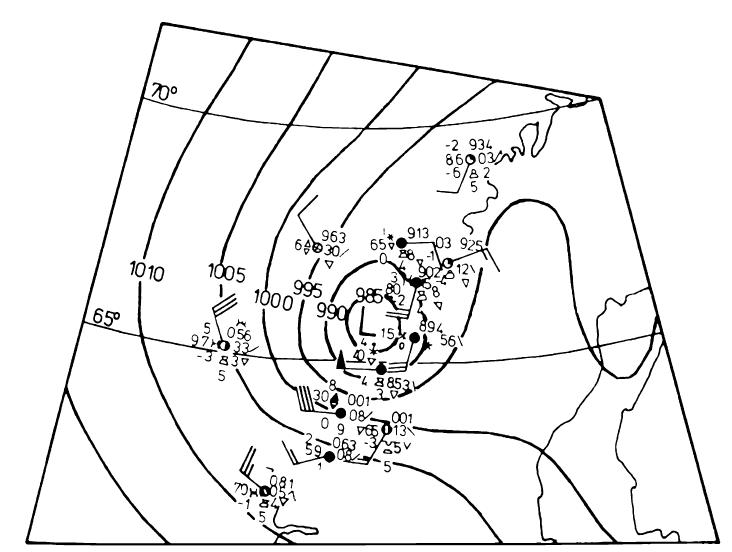
\includegraphics[width=0.5\linewidth]{{./chapters/figures_misc/polarlow1971}.jpeg}
  \caption{Синоптическая карта приземного анализа, показывающая наличие полярного мезоциклона в Норвежском море вблизи побережья Норвегии 13 октября 1971 г. \citep{RT2003}.}
  \label{fig:polarlow1971}
\end{figure}

Ярким примером является полярный мезомасштабный циклон, наблюдавшийся вблизи побережья Норвегии вблизи полярного круга 13 октября 1971 года \citep{Rasmussen1979}. На ранних стадиях его развития отмечалось большое количество энергии неустойчивости и формирование обширных систем глубокой конвекции, что привело к образованию осесимметричного вихря с теплым ядром, замкнутой циркуляцией диаметром несколько сотен километров и со скоростями приземного ветра, в среднем равными $25\mps$ (рис. \ref{fig:polarlow1971}).

Целью данной работы является исследование механизмов формирования полярных мезоциклонов на начальных стадиях их эволюции. Акцент сделан на воздействие параметров атмосферы, потому что динамика мезоциклонов любого типа зависит от благоприятных условий окружающей атмосферы. Будет показано, какое начальное состояние атмосферы благоприятно для генерации вихря в терминах изменения его кинетической энергии и падения приземного давления.

Для достижения поставленной в работе цели решаются следующие задачи:
\begin{sqlist}
\item Изучение зависимости характеристик полярного мезоциклона от внешних метеорологических параметров в их широком диапазоне. Одним из результатов решения задачи является определение области метеовеличин, благоприятной для интенсификации циклонического возмущения.
\item Выявление эффекта использования в модели той или иной параметризации турбулентного перемешивания в приводном и пограничном слоях атмосферы на динамику и структуру циркуляции.
\end{sqlist}

\section{Структура дипломной работы}
Дипломная работа состоит из введения, трех глав, заключения, библиографии и приложения. В первой главе на основе обзора литературы рассматриваются основные физические механизмы, объясняющие зарождение и эволюцию полярных мезоциклонов. Во второй главе описывается численная мезомасштабная модель ReMeDy, а именно система уравнений и используемые параметризации. Далее производится постановка стратегии исследования и выбор метода исследования. В частности, особое внимание уделяется энергетической диагностике. В четвертой главе приводятся результаты серий численных экспериментов, анализируются возникающие мезомасштабные циркуляции и объясняется их динамика. Кроме того, приводятся количественные оценки чувствительности интенсивности полярного мезоциклона к внешним параметрам атмосферы и к используемым параметризациям. В заключении содержатся основные выводы работы и обсуждается их теоретическая значимость. Приложение включают вывод системы уравнений мезомасштабной модели ReMeDy.


\end{document}
%\documentclass[12pt,a4paper]{report}
%
%%
% PACKAGES AND STYLES
%

% 
% Language and encoding
%
%\usepackage{mathtext}
%\usepackage[T2A]{fontenc}
\usepackage[utf8]{inputenc}
\usepackage[english,russian]{babel}
\usepackage{mmap}

%
% Colors
%
\usepackage[usenames]{color}
\usepackage{color}
\usepackage{colortbl}

%
% Symbols
%
\usepackage{amssymb}
\usepackage{MnSymbol}

%
% Units
%
%\usepackage[binary-units=true]{siunitx}
\newcommand{\km}{\mathrm{~\text{км}}}
\newcommand{\m}{\mathrm{~\text{м}}}
\newcommand{\s}{\mathrm{~\text{с}}}
\newcommand{\mps}{\m \s ^{-1}}
\newcommand{\pers}{\s ^{-1}}
\newcommand{\K}{\mathrm{~\text{К}}}
\newcommand{\Kpkm}{\K\km ^{-1}}
\newcommand{\hpa}{\mathrm{~\text{гПа}}}
\newcommand{\J}{\mathrm{~\text{Дж}}}
\newcommand{\Jpm}{\J \m ^{-3}}

%
% Paper size and margins
%
\usepackage{vmargin}
\setmarginsrb{2.5cm}{1cm}{2.5cm}{2cm}{0cm}{0cm}{0cm}{1.5cm}

%
% Page style
%
\usepackage{fancyhdr}
\setlength{\headheight}{16pt}
\newcommand{\changefont}{%
    \fontsize{9}{11}\selectfont
}
\fancyhf{}
\fancyhead[RO]{\changefont \slshape \rightmark} %section
\fancyhead[LO]{\changefont \slshape \leftmark} %chapter
\fancyfoot[C]{\changefont \thepage} %footer
\setlength{\headsep}{0.2in}
\pagestyle{fancy}

%
% Indenting
%
\usepackage{indentfirst}
\setlength{\parindent}{1cm}
\setlength{\parskip}{0.5cm}

%
% References
%
\usepackage{natbib}

%
% Hyperlinks
%
\usepackage[linktocpage=true,plainpages=false,pdfpagelabels=false]{hyperref}
\definecolor{linkcolor}{rgb}{0.1,0,0.9}
\definecolor{citecolor}{rgb}{0,0,0.9}
\definecolor{urlcolor}{rgb}{0,0,1}
\hypersetup{
    colorlinks, linkcolor={linkcolor},
    citecolor={citecolor}, urlcolor={urlcolor}
}

\bibliographystyle{plainnat}
% Bibliography: set article volume number in bold font
%\DeclareFieldFormat
%  [article]
%  {volume}{\textbf{#1}}
%\renewcommand\nameyeardelim{, }

%\usepackage{showkeys} % show labels

\newcommand{\figref}[1]{\mbox{Figure~\ref{#1}}}
\newcommand{\tabref}[1]{\mbox{Table~\ref{#1}}}
\newcommand{\secref}[1]{\mbox{Section~\ref{#1}}}
\newcommand{\chpref}[1]{\mbox{Chapter~\ref{#1}}}
\newcommand{\appref}[1]{\mbox{Appendix~\ref{#1}}}
\newcommand{\eqnref}[1]{\mbox{Eq.~(\ref{#1})}}
\newcommand{\listref}[1]{\mbox{Listing~(\ref{#1})}}

%
% Lists
%
\usepackage[shortlabels]{enumitem}

\newenvironment{sqlist}[1][\enskip$\filledsquare$]
        {\begin{itemize}[#1]}
        {\end{itemize}}

% New math commands
% differential d, from http://tex.stackexchange.com/a/60546/586
\newcommand*\diff{\mathop{}\!\mathrm{d}}
\newcommand\mean[1]{\overline{#1}}
\newcommand{\PDt}[2]{\partial #1/\partial #2}

%
% Tables
%
\usepackage{booktabs}
%\usepackage{tabularx}
\usepackage{tabu}
\usepackage{longtable}

%
% Figures
%
\usepackage{wrapfig}
\usepackage[font=small,textfont=it,labelfont=bf]{caption}
%\captionsetup[figure]{labelfont=bf}
\usepackage{tikz}
\usepackage{pgfplots}
\usetikzlibrary{calc}

%
% Equations
%
\usepackage{cool}

%
%\begin{document}
%\setcounter{chapter}{1}
\chapter{Механизмы генерации полярных мезоциклонов}
\label{sec:theory:intro}
Исследование структуры и динамики мезомасштабных вихрей высоких широт породило множество теорий их возникновения \citep{RT2003}. Схожесть изображений полярных мезоциклонов и тропических ураганов на спутниковых снимках дала повод считать, что в основе эволюции полярных вихрей также лежит конвекция. Однако благодаря накопленным натурным данным и результатам моделирования в конце XX века стала общепринятой точка зрения, согласно которой существует спектр полярных мезомасштабных вихрей. В одной части этого спектра находятся мезоциклоны, которые на снимках из космоса выглядят как спиралевидные системы облачности и в образовании которых преимущество имеют конвективные процессы. На другом конце спектра --- чисто бароклинные образования в виде облачных запятых, механизм образования которых аналогичен механизму внетропических циклонов синоптического масштаба.

Выдвижение единой теории, строго определяющей развитие мезоциклона, обычно не было успешным, так как мезоциклоны чаще всего возникают как гибридные образования. На разных этапах их развития преобладает тот или иной фактор.

Одним из кандидатов на роль механизма развития мезоциклона являются диабатические процессы, связанные, например, с выделением скрытого тепла кондесации, а также потоков тепла с поверхности. С 1970-х гг. значительный вес имеет концепция условной неустойчивости второго рода (conditional instability of second kind, CISK). Идея CISK заключается во взаимодействии мезомасштабных горизонтальных и вторичных вертикальных движений, приводящем к постепенному высвобождению энергии неустойчивости внешней среды. В конце 1980-х внимание исследователей переключилось на теорию неустойчивости взаимодействия атмосферы и океана (air-sea interaction instability, ASII), позднее обозначаемую термином WISHE (wind-induced surface heat exchange), предложенную в работе \citep{EmanuelRotunno1989}. Согласно этой теории, ключевую роль в усилении мезоциклона, то есть в падении давления в центре, играют запасы тепла у поверхности.

В то время как значительная часть исследований посвящена конвективным механизмам, не нужно преуменьшать важность бароклинных процессов. Этот подход основан на понятии бароклинной неустойчивости, возникающей вследствие температурного градиента между воздухом над относительно теплой поверхностью воды и воздухом над относительно холодной поверхностью, например, морским льдом. Авторы одной из пионерных работ, посвященных полярным мезоциклонам, рассматривают мезоциклоны именно как бароклинные возмущения \citep{HarroldBrowning1969}. В подтверждение приводятся данные наблюдений, свидетельствовавшие о том, что полярная депрессия имела в себе восходящую и нисходящую воздушную массу, повторяя структуру внетропических циклонов умеренных широт. Добавим, что полярные мезоциклоны бароклинного типа обычно разделяют на категории в зависимости от географического района происхождения. Так, например, полярные депрессии с обратным сдвигом впервые были обнаружены в регионе северо-западной Атлантики, где они чаще всего и встречаются.

Таковы основные механизмы образования полярных мезомасштабных циклонических вихрей. Что же их объединяет? Каждый из этих процессов можно рассмотреть с точки зрения генерации кинетической энергии атмосферных движений и ее источника в виде доступной потенциальной энергии (ДПЭ), которая по-своему накапливается в том или ином процессе.

\section{Бароклинная неустойчивость}
Как известно, волновую неустойчивость атмосферы можно разделить на два типа: баротропную --- связанную с горизонтальным сдвигом ветра --- и бароклинную, которая связана со сдвигом ветра по высоте. Бароклинная неустойчивость атмосферы возникает при условии бароклинности атмосферы, что означает зависимость плотности воздуха не только от давления, но и от температуры. Другими словами, температура не постоянна на изобарической поверхности.

\begin{figure}
  \centering
  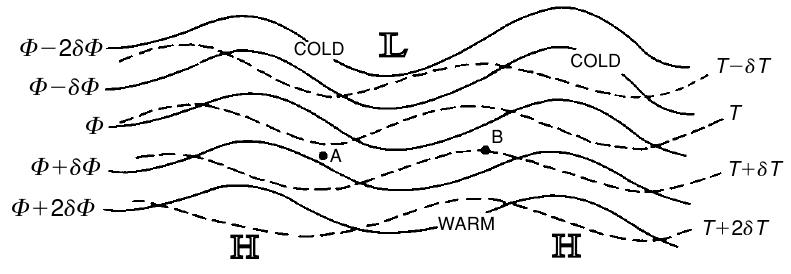
\includegraphics[width=\linewidth]{{./chapters/figures_misc/baroclinic_rt2003}.jpeg}
  \caption{Распределение изогипс (сплошные линии) и изотерм (пунктирные линии) на изобарической поверхности в развивающейся бароклинной волне в Северном полушарии \citep{RT2003}.}
  \label{fig:baroclinic_rt2003}
\end{figure}

В атмосфере средний поток, связанный с горизонтальным температурным градиентом на изобарических поверхностях, обладает доступной потенциальной энергией, которая может быть трансформирована в кинетическую, что вызовет спонтанный рост малых возмущений.

Принцип развития бароклинной волны в регионе с сильным температурным градиентом может быть объяснен следующим образом (рис. \ref{fig:baroclinic_rt2003}). Пусть в изначально зональном воздушном потоке возникает возмущение в виде слабой волны. Тогда появятся меридиональные составляющие потока, которые приведут к возмущению поля зонально-ориентированных изотерм. Фаза волны в поле температуры будет на одну четвертую длины волны отличаться от фазы волны в поле давления (или геопотенциала). При отсутствии других факторов горизонтальная адвекция температуры, связанная с геострофическим ветром, будет и далее возмущать поле изотерм, удаляя их от начального положения, и способствовать росту волны. При этом в точке A будет наблюдаться нисходящие движения холодного воздуха, а в точке B --- подъем теплого воздуха, что означает опускание центра тяжести системы и рост кинетической энергии.

Первой работой, в которой была применена бароклинная модель, является исследование 1974 г. Мэнсфилда \citep{RT2003}, который использовал данные наблюдений мезоциклона, рассмотренного еще в пионерной работе Хэррольда и Браунинга. Для выявления скорости роста и длины волны как главных характеристик возмущений в плоскопараллельном потоке Мэнсфилд применил линейную модель Иди. Результаты довольно близки к реальности, причем длина волны самой быстрой моды пропорциональна радиусу деформации Россби. Это говорит о том, что размеры полярной депрессии, предсказанные расчетами по линейной модели, невелики из-за малой протяженности по высоте. При этом, однако, не учитывались ни трение, ни потоки тепла с поверхности. Как показал сам Мэнсфилд, эти факторы стремятся подавить растущую волну, а выделение скрытого тепла в атмосфере, наоборот, увеличивает скорость роста.

Объектом другого теоретического исследования бароклинной неустойчивости в нижней тропосфере являются мезомасштабные циклоны в Японском море \citep{TsubokiWakahama1992}. Авторы провели линейный анализ, результаты которого согласуются со спутниковыми снимками, свидетельствующими о том, что в выбранном районе наблюдается два типа мезоциклона ($200$--$300\km$ и $500$--$700\km$). Им соответствуют две главные моды неустойчивости. Кроме того, было доказано, что обе бароклинные моды растут за счет увеличения ДПЭ и ее конвертации в кинетическую энергию.

Бароклинность атмосферы была предложена для объяснения роста полярных мезоциклонов и в работе Дункана за 1977 г. \citep{RT2003}. В ней утверждается, в частности, что полярные депрессии обычно являются низкими бароклинными образованиями, в которых переход энергии из доступной потенциальной в кинетическую происходит в нижних $200$--$300\hpa$ атмосферы.

Постепенно многие авторы пришли к выводу о том, что механизм бароклинной неустойчивости недостаточно правильно предсказывает динамику полярных мезоциклонов. Точнее, моды бароклинной неустойчивости имели сходные с наблюдениями волновые числа, но их скорость роста часто оказывалась неправильной. Тогда был предложен эффект выделения теплоты конденсации как фактор, увеличивающий протяженность возмущений по высоте и, следовательно, замедляющий их скорость.

Во введении было сказано несколько слов о важности высотной ложбины, выступающей в качестве триггерного механизма при взаимодействии с бароклинной неустойчивостью в нижних слоях тропосферы. Многими авторами отмечается, что это взаимодействие ограничивается некоторыми факторами. Например, для этого необходимо, чтобы низкая арктическая воздушная масса должна приобрести некоторую неустойчивость под влиянием подстилающей поверхности. Кроме того, возникает вопрос о способности слишком тонких бароклинных зон служить источником энергии для роста мезоциклонов \citep{AlbrightEtAl1995}.

Тем не менее, нередки случаи, когда в верхней тропосфере присутствует достаточно обширная депрессия, а бароклинная зона достаточно высокая. Такими условиями характеризуется два случая полярных мезоциклонов в Норвежском море, описанные в \citep{Nordeng1990}. Автор указывает на взаимное влияние главной бароклинной зоны (полярного фронта) и 'фиксированного поверхностного форсинга' температурных неоднородностей на границе морского льда и воды.

Говоря о последнем десятилетии, значительный вклад в изучение полярных мезоциклонов японские исследователи \citep{YanaseEtAl2004,YanaseNiino2004,Nagata1993}, из которых выделяется работа \citep{YanaseNiino2007}. Ее авторы обнаруживают показывают чувствительность структуры полярного мезоциклона к степени бароклинности окружающей атмосферы. Кроме экспериментов, в которых учитывался лишь сдвиг ветра с высотой (как критерий бароклинности) были проведена серия экспериментов с учетом фазовых переходов влаги и потоков энергии с поверхности океана. Это помогло понять зависимость скорости роста вихря и его энергетики от разных физических параметров атмосферы. 

Работа \citep{YanaseNiino2007} выступает как одна из наиболее близких к нашим исследованиям по постановке задачи и используемым методам. Отличительной особенностью данной дипломной работы по сравнению с указанной является то, что акцент сделан на развитии вихря из аномалии тепла мелкого масштаба вблизи поверхности, в то время как в \citep{YanaseNiino2007} исследовалось поведение уже изначально аналитически заданного осесимметричного вихря. Второй отличительной чертой являются фоновые атмосферные условия, определяющие тип неустойчивости: в нашей работе рассматривается термическая неустойчивость (см. \ref{sec:theory:thermal}), а в указанной японской статье важнейшая роль принадлежит бароклинная неустойчивость.

\section{Баротропная неустойчивость}
Другим видом волновой неустойчивости в атмосфере является баротропная неустойчивость, которая в отличие от бароклинной неустойчивости, играет гораздо меньшую роль в генерации полярных мезомасштабных депрессий. Поэтому лишь коротко рассмотрим ее особенности.

\begin{figure}
  \centering
  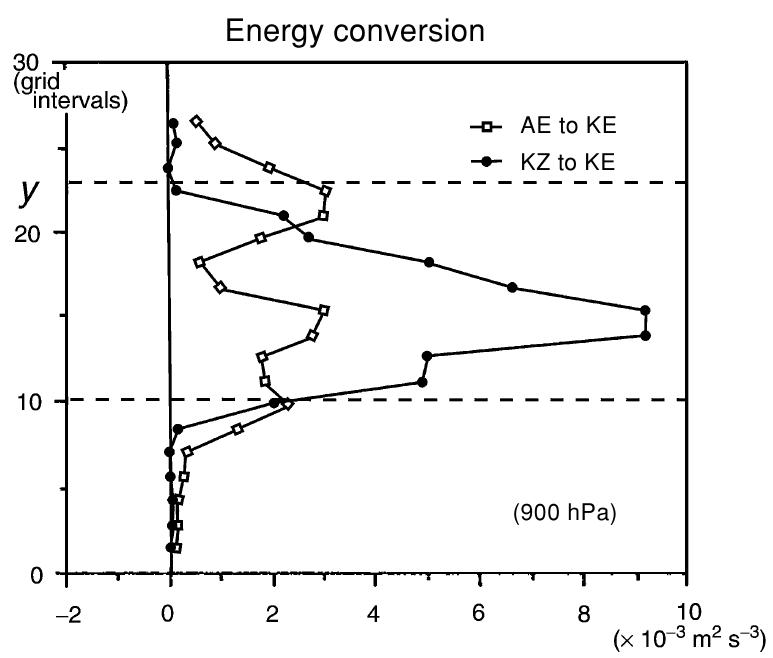
\includegraphics[width=0.5\linewidth]{{./chapters/figures_misc/barotropic_nagata1993}.jpeg}
  \caption{Бароклинная и баротропная конверсия энергии на уровне $900\hpa$ \citep{Nagata1993}.}
  \label{fig:barotropic_nagata1993}
\end{figure}

Согласно \citep{Holton2004}, баротропная неустойчивость --- это волновая неустойчивость, связанная с горизонтальным сдвигом ветра в струйном потоке. Источник роста баротропных возмущений --- кинетической энергии среднего потока.

Подробное исследование полярных мезоциклонов с точки зрения баротропной неустойчивости было проведено, например, для района конвергенции полярной воздушной массы над Японским морем \citep{Nagata1993}. В указанной работе автор отмечает, что в зоне шириной всего несколько десятков километров наблюдаются максимумы завихренности. Для их исследования он применил численную атмосферную модель, которая воспроизвела волны в поле потенциального вихря, которые постепенно обострялись и приобретали вид полярных депрессий с аномалией давления $2$--$4\hpa$. Вихри имели спиралевидную структуру с теплым ядром в центре.

Для подтверждения гипотезы о баротропности наблюдаемых процессов Нагата сопоставляет бароклинный и баротропный источники энергии в полосе вблизи вихря. Пусть $u'$ и $v'$ --- отклонения компонент скорости от среднего потока, то для кинетической энергии формула выглядит следующим образом:
\begin{equation}
K_E = \overline{\frac{1}{2}\left(u'^2 + v'^2\right)}
\end{equation}
Баротропный и бароклинный вклады в трансформацию энергии вычисляются по выражениям
\begin{equation}
C(K_M,K_E)=-\overline{u'v'}\frac{d\overline{u}}{y}
\end{equation}
и
\begin{equation}
C(A_E,K_E)=-\overline{\omega'\alpha'},
\end{equation}
где $K_M$, $K_E$ и $A_E$ --- средняя кинетическая энергия, кинетическая энергия возмущений и доступная потенциальная энергия возмущений соответственно, $\omega'$ --- отклонения вертикальной скорости, $\alpha'$ --- отклонения удельного объема, горизонтальная черта означает осреднение по области.

На рис. \ref{fig:barotropic_nagata1993} представлено распределение интенсивности трансформации энергии по горизонтали. Сравнивая с профилем горизонтального сдвига ветра и профилем кинетической энергии, автор делает вывод, что основным источником вихревых движений является именно сдвиг ветра, чей максимум совпадает с максимумом кинетической энергии. Вклад бароклинной компоненты, как видно из рисунка, по крайней мере в два раза меньше.

Роли баротропных волн в полярном циклогенезе были посвящены и другие работы, объектом которых являлись мезоциклоны в Северной Атлантике и в Беринговом море. К примеру, Дункан, оценивая механизмы развития трех полярных мезоциклонов \citep{RT2003}, заключил, что роль баротропных процессов незначительна. Хотя большинство исследований основывались на структуре полярного струйного течения, Рид \citep{ReedDuncan1987} отмечал, что формирование достаточно резких сдвигов ветра над океанами зимой для развития мезомасштабных вихрей маловероятно.

Итак, атмосферные баротропные волны сами значимы в аспекте образования полярных мезоциклонов по сравнению с бароклинной и термической неустойчивостью (см. следующий раздел). Тем не менее, баротропная неустойчивость иногда может действовать вместе с другими механизмами и даже выступать как триггерный процесс.

\section{Термическая неустойчивость}
Как было сказано во введении, в нашем исследовании важнейшим фактором развития вихря являются конвективные процессы, иначе интерпретируемые как выделение энергии термической неустойчивости. Последние несколько десятилетий ведутся споры по вопросу, каким именно путем конвекция влияет на эволюцию полярных вихрей. В первых работах в этом направлении полярный мезоциклон представлялся даже как одно большое кучеводождевое облако. Однако затем фокус исследований сместился в сторону механизмов бароклинной неустойчивости. Теория конвективных механизмов применительно к этим вихрям была возвращена на первый план в работе \citep{Okland1987,Rasmussen1979}, в которой авторы рассматривают полярный мезоциклон с точки зрения условной неустойчивости второго рода (conditional instability of second kind, CISK), ранее использовавшаяся при изучении тропических ураганов. На смену CISK была предложена улучшенная концепция, называемая WISHE, которая объясняет динамику мезоциклонов через взаимодействие циркуляции циклона и потоков тепла на поверхности. Эти теории подробнее рассмотрены ниже.

\label{sec:theory:cisk_wishe}
\subsection{Условная неустойчивость второго рода}
\subsubsection{Понятие условной неустойчивости}
Динамическая неустойчивость в атмосфере Земли часто связана с неустойчивостью частицы или слоя, то есть определяющее значение имеет сила плавучести. Одним из механизмов, предложенных для объяснения полярных мезоциклонов, является условная неустойчивость второго рода (CISK). 

Условная неустойчивость – понятие, близкое к статической неустойчивости, и также базируется на разности плотности между частицей воздуха и окружающей атмосферы. Основное отличие состоит в том, что при определении условной неустойчивости принимается во внимание насыщенность воздуха, в то время как статическая устойчивость предполагает влажность равную либо $0$, либо $100\%$. Критерием условной неустойчивости является вертикальный градиент псевдопотенциальной температуры (эквивалентной потенциальной температуры при насыщении).

Помимо обычного взгляда на условную неустойчивость в терминах градиентов потенциальной температуры, в контексте данной работы необходимо привести 'энергетическое' определение, в котором используется понятие конвективной доступной потенциальной энергии (convective available potential energy, CAPE):
\begin{equation}
CAPE_i = \int_{z_{i}}^{z{LNB}} g\frac{T-\overline{T}}{T}dz,
\end{equation}
где $CAPE_i$ --- конвективная доступная потенциальная энергия частицы, $z_{i}$ --- высота, на которой находится частица, $z_{LNB}$ --- уровень нейтральной плавучести, $T$ --- температура частицы, $\overline{T}$ --- температура окружающего воздуха. То есть частица воздуха обладает условной неустойчивостью при положительной энергии плавучести ($CAPE_i>0$). Точнее, для ненасыщенного воздуха устойчивость может быть в двух вариантах: 1) $CAPE=0$: устойчивость для всех вертикальных движений, 2) $CAPE>0$: неустойчивость для вертикальных движений конечной амплитуды, которая, в свою очередь, может быть двух типов: $CAPE>CIN$ и $CIN>CAPE$ \citep{Lin2007}.

Минусом метода частицы является неспособность описать неустойчивости, связанные с горизонтальным градиентом температуры (бароклинную и баротропную неустойчивость). Кроме того, в ней не учитываются некоторые процессы, уменьшающие силу плавучести, а именно эффект вовлечения, влияние конденсированной влаги на плотность воздуха и компенсирующие движения окружающего воздуха в ответ на формирование облаков.

\subsubsection{Условная неустойчивость второго рода}
Некоторые из указанных процессов включены в концепцию условной неустойчивости второго рода (CISK). Она была впервые применена Чарни и Элиассеном в работе по тропическому циклогенезу и подразумевает следующее:
\begin{sqlist} 
\item Выделение скрытого тепла при конвекции приводит к образованию циклонического возмущения в нижней тропосфере.
\item Циклоническая аномалия создает условия для конвергенции влаги благодаря трению в пограничном слое (Экмановская подкачка).
\item Конвергенция потоков способствует подъему условно неустойчивого воздуха на уровень свободной конвекции и выделению скрытого тепла конденсации.
\end{sqlist}
Принципиальная схема условной неустойчивости второго рода показана на рис. \ref{fig:cisk_rt2003}.

Роль глубокой конвекции в эволюции полярных мезоциклонов подчеркивалась в работах Расмуссена и Окланда \citep{RT2003}. Они справедливо заявляли, что устойчивость арктических воздушных масс резко уменьшается при холодных вторжениях на поверхность океана.

\begin{figure}[!ht]
	\centering
	\begin{subfigure}[t]{0.4\textwidth}
		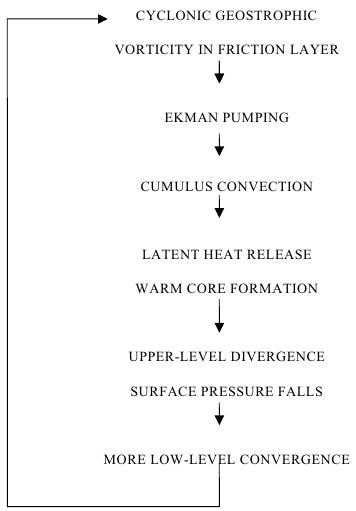
\includegraphics[width=\linewidth]{{./chapters/figures_misc/cisk_rt2003}.jpeg}
		\caption{ }
		\label{fig:cisk_rt2003}
	\end{subfigure}
	\hfill
	\begin{subfigure}[t]{0.4\textwidth}
		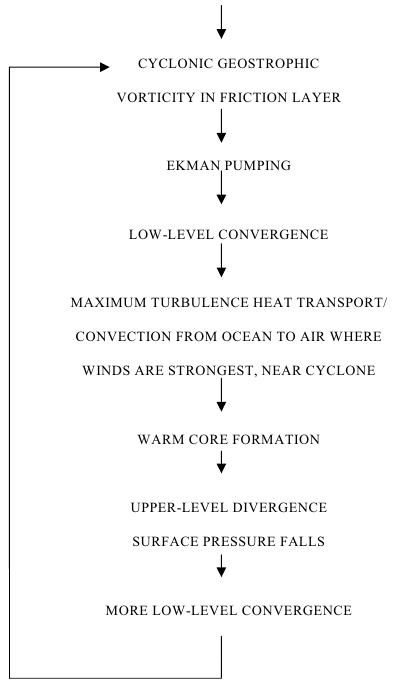
\includegraphics[width=\linewidth]{{./chapters/figures_misc/wishe_rt2003}.jpeg}
		\caption{ }
		\label{fig:wishe_rt2003}
	\end{subfigure}
	\caption{Принципиальная схема CISK (a) и WISHE (b) \citep{RT2003}.}
\end{figure}

Теоретические исследования были продолжены с применением сначала аналитической модели \citep{SardieWarner1983} в двумерных квазигеострофических уравнениях, учитывающих диабатические источники тепла. После сравнения с данными наблюдений семи случаев было показано, что эффектов CISK недостаточно для описания скорости роста ни атлантических мезоциклонов, ни тихоокеанских. С другой стороны, недостаточно и влияние только 'сухой' бароклинности. Однако при суперпозиции условной неустойчивости и бароклинности результаты оказываются близкими к реальности. При этом наилучшее совпадение с наблюдениями показывают те результаты, включающие эффекты CISK во влажной бароклинной атмосфере. Этот в некоторой степени очевидный факт объясняется тем, что при наложении бароклинности и конвективной неустойчивости тепло выделяется как в кучевой, так и в слоистой облачности. Другими словами, в нижних слоях атмосферы существует источник бароклинной доступной потенциальной энергии, который дополняется на высотах источником энергии фазовых переходов. Выводы, сделанные в аналитическом подходе к проблеме, подтверждаются ре-зультатами численного моделирования \citep{SardieWarner1983}.

Одной из новейших работ, посвященных анализу динамики полярных мезоциклонов с точки зрения конвективной доступной потенциальной энергии является статья \citep{LindersSaetra2010}. В ней с помощью набора данных, полученных в ходе эксперимента в Северном море, доказывается, что, во-первых, условная неустойчивость фактически отсутствует, а во-вторых, опять же в контексте полярных мезоциклонов величина CAPE сравнима с потоком тепла с поверхности океана за ограниченное время и, таким образом, не представляет важного компонента бюджета энергии мезоциклона.

\subsection{WISHE}
На замену теории неустойчивости второго рода пришла теория интенсификации циклона под действием потоков тепла с поверхности \citep{EmanuelRotunno1989}. В данной концепции предполагается, что атмосфера нейтрально устойчива по отношению к влажной конвекции. Это верно для районов формирования тропических циклонов, для которых и разрабатывалась данная теория. Влажная конвекция перемешивает нижние слои тропосферы, но не приводит к образованию значительной температурной аномалии в случае отсутствия источника явного или скрытого тепла с поверхности. Потоки тепла с поверхности зависят от скорости ветра и, следовательно, определяются интенсивностью вращения вихря. Другими словами, имеется четкая обратная связь между интенсивностью мезоциклона и нагревом от подстилающей поверхности \ref{fig:wishe_rt2003}.

Можно заметить, что отличие теории WISHE от приведенной в предыдущем разделе состоит в том, каким образом связана конвекция с интенсивностью циклона. То есть в случае WISHE максимальная неустойчивость наблюдается в районах с максимальным ветром и не включает совместного влияния конвергенции под действием силы трения.

По современным представлениям, WISHE остается одной из наиболее продвинутых концепций в теории генезиса как тропических \citep{CraigGray1996}, так и полярных вихрей \citep{EmanuelRotunno1989}. Тем не менее, этот механизм имеет свои недостатки, в частности, предположение о градиентном балансе в пограничном слое, а также об осесимметричности вихря. И теория CISK, и теория WISHE не описывают процесс зарождения возмущения. Например, Эмануэль citep{EmanuelRotunno1989} отмечает, что для поддержания WISHE атмосферный вихрь уже должен существовать в виде возмущения конечной амплитуды.

\section{Влияние подстилающей поверхности на развитие полярных мезоциклонов}
В атмосфере полярных регионов как бароклинные, так и конвективные процессы часто наблюдаются вблизи границы льда или снежного покрова. Они связаны с температурным градиентом между охлажденной поверхностью льда и относительно теплой поверхностью воды, достигающим несколько десятков градусов. Также возникают значительные контрасты альбедо и шероховатости. Из-за этого энергетический бюджет пограничного слоя над открытой водой и над поверхностью льда существенно отличается.

\begin{figure}
  \centering
  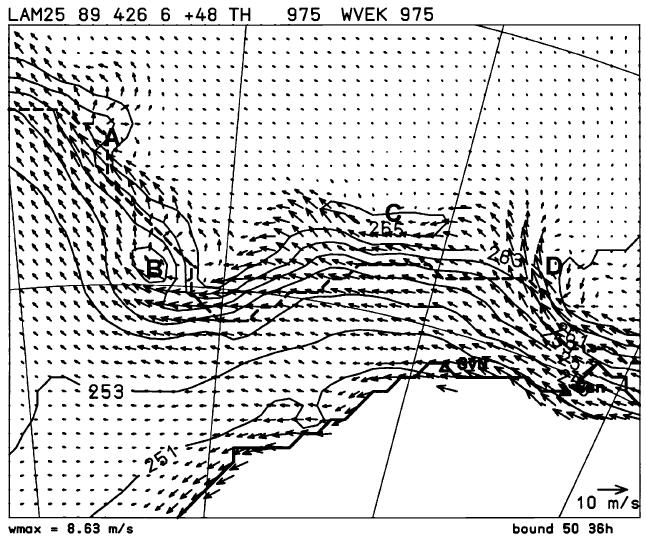
\includegraphics[width=0.5\linewidth]{{./chapters/figures_misc/heinemann1996a}.jpeg}
  \caption{Потенциальная температура (сплошные линии через $2\K$) и вектора скорости на уровне $975\hpa$. Буквами обозначены отдельные мезоциклоны \citep{RT2003}.}
  \label{fig:heinemann}
\end{figure}

Удобная для генерации мезоциклонов резкая бароклинная зона, или фронт пограничного слоя (ФПС) часто формируется, когда воздушный поток направлен почти параллельно границе ледового покрова. Процессы фронтогенеза ведут к образованию облачных валиков, что четко видно на спутниковых снимках. В результате отклонений поля ветра от среднего полярный может происходить адвекция ФПС. Тогда создаются благоприятные условия для формирования вихря. Полярные мезоциклоны такого типа классифицируются как системы на Арктическом/Антарктическом фронте и питаются за счет бароклинной неустойчивости и мощных потоков тепла с поверхности воды.

В данном разделе коротко обсуждаются результаты исследований за последние два десятилетия, в которых предметом являлось взаимодействие поверхности океана, частично покрытой льдом, и динамики мезоциклона, зарождающегося или переносящегося над этой областью.

Одним из первых данной проблемой занялся Хайнеманн \citep{Heinemann1997}, используя модель NORLAM, проводивший идеализированные эксперименты для конкретной территории, а именно моря Уэделла. Изначально однородные по горизонтали метеополя были деформированы в результате поверхностного форсинга, что выразилось, в частности в падении давления в поясе вдоль границы льда. Это сопровождалось резким усилением скорости ветра, образования зоны конвергенции над водой и температурного градиента около $5\K$ на $50\km$.

При этом геострофическая компонента скорости ветра была направлена квазипараллельно фронту, агеострофическая --- со льда на воду. Граница льда была построена по данным наблюдений и в ледовом покрове существовали неоднородности в виде заливов и выступов. Именно в этих областях, как и ожидалось, возникали условия для генерации завихренности \ref{fig:heinemann}. Однако, как доказывает автор, возникшая серия вихрей состояла из мезоциклонов, слабо развитых по высоте и не прослеживающихся на уровне $700\hpa$ даже через трое суток моделирования.

Похожее исследование, основанное на данных натурных измерений, было проведено и для Гудзонова залива \citep{AlbrightEtAl1995}. В одном из экспериментов температура поверхности океана (ТПО) была увеличена на $8\K$, что привело к серьезному усилению полярного вихря до скоростей, превышающих ураганные значения. Кроме влияния ТПО, авторы обнаружили сильную зависимость динамики мезоциклона от формы границы льда: при замене реальной границы на идеально прямую меридионально расположенную, вихрь существенно поменял свою траекторию и уменьшил скорость своего роста.

Что касается температуры поверхности, то ее влияние на эволюцию мезоциклона было проанализировано в работе \citep{AdakudluBarstad2011}. В ней показано, что аномалия давления в центре полярной депрессии росла в зависимости от вариаций ТПО со скоростью около $2\hpa\K^{-1}$.

\begin{figure}
  \centering
  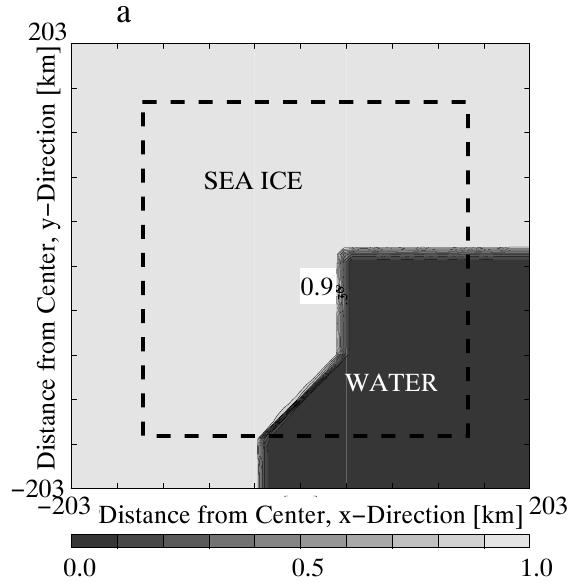
\includegraphics[width=0.5\linewidth]{{./chapters/figures_misc/ds2005}.jpeg}
  \caption{Распределение льда и воды в экспериментах \citep{DiererSchluenzen2005}.}
  \label{fig:ds2005}
\end{figure}

Более идеализированное исследование \citep{DiererSchluenzen2005} было призвано оценить взаимодействие между мезоциклоном и  параметрами ледяного покрова, включая толщину льда, соотношение льда и воды на единице площади и др. Форма границы льда была одной и той же для всех экспериментов и имела вид угловой ступеньки в юго-восточной части области интегрирования \ref{fig:ds2005}. В отличие от многих других работ, здесь явно учитывались и процессы в океане, а наличие морского течения.
 
Наиболее важным параметром оказалось распределение льда, которое определяет градиент температуры между поверхностью и приземным слоем воздуха. Кроме того, наименьший средний поток тепла наблюдался при смещенном треке мезоциклона. Морское течение и толщина льда почти не влияют на тенденцию давления. Наибольшие отличия тенденции давления по сравнению с контрольным экспериментом наблюдаются в эксперименте с однородным льдом и со смещенным треком. В первом случае мезоциклон сам 'сдвигает' лед, и в результате в районе неоднородной концентрации льда развивается бароклинный слой.

Говоря о результатах указанной работы, отметим, что параметры, влияющие на вариации давления и скорости ветра, проявляются и в значимых изменениях потоков тепла с поверхности. Влиянием мелкомасштабных изменений потоков (из-за толщины льда или морских течений) можно пренебречь. Менее плотный ледовый покров (с присутствием пятен открытой воды) и большие скорости ветра являются благоприятными условиями для дальнейшего разрежения льда и возникновению положительной обратной связи.

%\begin{thebibliography}{12}
 \bibitem{ER89}
Emanuel KA, Rotunno R. 1989. Polar lows as Arctic hurricanes. \textit{Tellus} \textbf{41A:} 1-17.
\end{thebibliography}
%
%\end{document}
\documentclass[12pt,a4paper]{report}

%
% PACKAGES AND STYLES
%

% 
% Language and encoding
%
%\usepackage{mathtext}
%\usepackage[T2A]{fontenc}
\usepackage[utf8]{inputenc}
\usepackage[english,russian]{babel}
\usepackage{mmap}

%
% Colors
%
\usepackage[usenames]{color}
\usepackage{color}
\usepackage{colortbl}

%
% Symbols
%
\usepackage{amssymb}
\usepackage{MnSymbol}

%
% Units
%
%\usepackage[binary-units=true]{siunitx}
\newcommand{\km}{\mathrm{~\text{км}}}
\newcommand{\m}{\mathrm{~\text{м}}}
\newcommand{\s}{\mathrm{~\text{с}}}
\newcommand{\mps}{\m \s ^{-1}}
\newcommand{\pers}{\s ^{-1}}
\newcommand{\K}{\mathrm{~\text{К}}}
\newcommand{\Kpkm}{\K\km ^{-1}}
\newcommand{\hpa}{\mathrm{~\text{гПа}}}
\newcommand{\J}{\mathrm{~\text{Дж}}}
\newcommand{\Jpm}{\J \m ^{-3}}

%
% Paper size and margins
%
\usepackage{vmargin}
\setmarginsrb{2.5cm}{1cm}{2.5cm}{2cm}{0cm}{0cm}{0cm}{1.5cm}

%
% Page style
%
\usepackage{fancyhdr}
\setlength{\headheight}{16pt}
\newcommand{\changefont}{%
    \fontsize{9}{11}\selectfont
}
\fancyhf{}
\fancyhead[RO]{\changefont \slshape \rightmark} %section
\fancyhead[LO]{\changefont \slshape \leftmark} %chapter
\fancyfoot[C]{\changefont \thepage} %footer
\setlength{\headsep}{0.2in}
\pagestyle{fancy}

%
% Indenting
%
\usepackage{indentfirst}
\setlength{\parindent}{1cm}
\setlength{\parskip}{0.5cm}

%
% References
%
\usepackage{natbib}

%
% Hyperlinks
%
\usepackage[linktocpage=true,plainpages=false,pdfpagelabels=false]{hyperref}
\definecolor{linkcolor}{rgb}{0.1,0,0.9}
\definecolor{citecolor}{rgb}{0,0,0.9}
\definecolor{urlcolor}{rgb}{0,0,1}
\hypersetup{
    colorlinks, linkcolor={linkcolor},
    citecolor={citecolor}, urlcolor={urlcolor}
}

\bibliographystyle{plainnat}
% Bibliography: set article volume number in bold font
%\DeclareFieldFormat
%  [article]
%  {volume}{\textbf{#1}}
%\renewcommand\nameyeardelim{, }

%\usepackage{showkeys} % show labels

\newcommand{\figref}[1]{\mbox{Figure~\ref{#1}}}
\newcommand{\tabref}[1]{\mbox{Table~\ref{#1}}}
\newcommand{\secref}[1]{\mbox{Section~\ref{#1}}}
\newcommand{\chpref}[1]{\mbox{Chapter~\ref{#1}}}
\newcommand{\appref}[1]{\mbox{Appendix~\ref{#1}}}
\newcommand{\eqnref}[1]{\mbox{Eq.~(\ref{#1})}}
\newcommand{\listref}[1]{\mbox{Listing~(\ref{#1})}}

%
% Lists
%
\usepackage[shortlabels]{enumitem}

\newenvironment{sqlist}[1][\enskip$\filledsquare$]
        {\begin{itemize}[#1]}
        {\end{itemize}}

% New math commands
% differential d, from http://tex.stackexchange.com/a/60546/586
\newcommand*\diff{\mathop{}\!\mathrm{d}}
\newcommand\mean[1]{\overline{#1}}
\newcommand{\PDt}[2]{\partial #1/\partial #2}

%
% Tables
%
\usepackage{booktabs}
%\usepackage{tabularx}
\usepackage{tabu}
\usepackage{longtable}

%
% Figures
%
\usepackage{wrapfig}
\usepackage[font=small,textfont=it,labelfont=bf]{caption}
%\captionsetup[figure]{labelfont=bf}
\usepackage{tikz}
\usepackage{pgfplots}
\usetikzlibrary{calc}

%
% Equations
%
\usepackage{cool}


\begin{document}
\setcounter{chapter}{2}
\chapter{Численные эксперименты}
\label{ch:experiments}
\section{Мезомасштабная модель ReMeDy}
Оригинальная версия модели \citep{MillerWhite1984,XueThorpe1991} основана на двумерном представлении прогностических уравнений с использованием $\sigma$-координаты; в дальнейшем наряду с модификацией граничных условий и включением эффектов вращения была преобразована в трехмерную \citep{MirandaPhD}. Данная модель использовалась при исследовании ледового бриза \citep{ChechinEtAl2013} и в настоящее время развивается в Научно-исследовательском вычислительном центре МГУ. Современное состояние модели изложено в виде табл. \ref{tab:model}

\renewcommand{\arraystretch}{2}
\begin{table}
\centering
\caption{Характеристики модели ReMeDy}
\label{tab:model}
\small
\begin{tabu} to \textwidth {p{5cm}X[l]}
\toprule
Система уравнений & Негидростатическая, трехмерная \\
Учет силы Кориолиса & Приближение $f$-плоскости \\
Радиация & Блок переноса коротковолновой и длинноволновой радиации CLIRAD-SW и CLIRAD-LW (ссылки в \citep{StepanenkoMikushin2008})\\
Примеси & Блок переноса атмосферной примеси \citep{StepanenkoMikushin2008} \\
Турбулентное замыкание	& Локальное замыкание Смагоринского-Лилли \citep{Smagorinsky1958,Lilly1962}, нелокальное замыкание Люпкеса-Шлюнцен \citep{LupkesSchluenzen1996,NohEtAl2003} \\
Подстилающая поверхность & Модель деятельного слоя ИВМ РАН \citep{VolodinLykosov1998} \\
Параметризация водоемов (поверхностного слоя океана)	& Одномерная модель водоема LAKE \citep{StepanenkoEtAl2011} \\
Фазовые переходы воды & Параметризация микрофизики облаков и осадков при положительной температуре \citep{TeixeiraMiranda1997}\\
Вертикальная координата & $\sigma=\frac{p-p_{top}}{p_*}$, где $p_*=p_{surf}-p_{top}$, $p_{surf}$ -- давление на земной поверхности, $p_{top}$ -- давление на верхней границе расчетной области \\
Боковые граничные условия & Периодические, однородные Неймана, Дирихле, излучения \\
Верхнее и нижнее граничные условия & Однородное условие Неймана для горизонтальных составляющих скорости, условия Дирихле для вертикальной скорости; для температуры и примесей задаются потоки на поверхности \\
Рэлеевское трение в буферной зоне & Применяется к сеточному решению вблизи верхней и горизонтальных границ области. Это позволяет частично подавить схемные возмущения, возникающие около границ. С помощью тригонометрической функции обеспечивается притяжение метеорологических полей к значениям на внутренней границе буферной зоны или к фоновому состоянию. \\
Дискретизация производных & По пространству: схема центральных разностей, по времени: явная схема второго порядка 'чехарда' \\
Численная фильтрация & Пространственный фильтр 4-го порядка для подавления волн (максимально – с длиной в два шага сетки), фильтр Аселина для подавления временной вычислительной моды \\
Пространственная сетка & $C$-сетка Аракавы (см. \ref{sec:model:grid})\\
\bottomrule
\end{tabu}
\end{table}

\subsection{Система уравнений}
Вывод системы уравнений модели представлен в \ref{app:A}. Чтобы улучшить свойства численного решения, прогностические уравнения модели написаны в потоковой форме. Это позволяет представить адвективные слагаемые в форме дивергенции соответствующего вектора потока. После интегрирования по расчетной области, вклад этих слагаемых проявляется через граничные условия, что исключает ложную генерацию энергии в пределах этой области и тем самым позволяет контролировать нелинейную неустойчивость. Полная система прогностических уравнений в потоковой форме выглядят так:
\begin{subequations}\label{eq:progn0}
\begin{align}
\frac{\partial{up_*}}{\partial{t}} + \frac{\partial{u^2p_*}}{\partial{x}}+ \frac{\partial{vup_*}}{\partial{y}}+ \frac{\partial{\dot{\sigma}up_*}}{\partial{\sigma}}&=-p_* \frac{\partial{\phi'}}{\partial{x}}+\sigma \frac{\partial{p_*}}{\partial{x}}\frac{\partial{\phi'}}{\partial{\sigma}}+f(v-V_g )p_*+p_*(D_u+R_u )\label{eq:progn1} \\
\frac{\partial{vp_*}}{\partial{t}} + \frac{\partial{uv^2p_*}}{\partial{x}}+ \frac{\partial{v^2p_*}}{\partial{y}}+ \frac{\partial{\dot{\sigma}vp_*}}{\partial{\sigma}}&=-p_* \frac{\partial{\phi'}}{\partial{y}}+\sigma \frac{\partial{p_*}}{\partial{y}}\frac{\partial{\phi'}}{\partial{\sigma}}-f(u-U_g )p_*+p_*(D_v+R_v )\label{eq:progn2} \\
\frac{\partial{\tilde{w}p_*}}{\partial{t}} + \frac{\partial{u\tilde{w}p_*}}{\partial{x}}+ \frac{\partial{v\tilde{w}p_*}}{\partial{y}}+ \frac{\partial{\dot{\sigma}\tilde{w}p_*}}{\partial{\sigma}}&=S_vp_*\frac{\partial{\phi'}}{\partial{\sigma}}+p_*g(\frac{\theta'}{\theta_S}-q_r)+p_*(D_{\tilde{w}}+R_{\tilde{w}})\label{eq:progn3} \\
\frac{\partial{\theta'p_*}}{\partial{t}} + \frac{\partial{u\theta'p_*}}{\partial{x}}+ \frac{\partial{v\theta'p_*}}{\partial{y}}+ \frac{\partial{\dot{\sigma}\theta'p_*}}{\partial{\sigma}}&=S_v\tilde{w}p_* \frac{\partial{\theta_s}}{\partial{\sigma}}+p_*Q+p_*(D_{\theta}+R_{\theta})\label{eq:progn4} \\
\frac{\partial{p_*}}{\partial{t}} + \frac{\partial{up_*}}{\partial{x}}+ \frac{\partial{vp_*}}{\partial{y}}+ \frac{\partial{\dot{\sigma}p_*}}{\partial{\sigma}}&=0\label{eq:progn5} \\
\frac{\partial{q_vp_*}}{\partial{t}} + \frac{\partial{uq_vp_*}}{\partial{x}}+ \frac{\partial{vq_vp_*}}{\partial{y}}+ \frac{\partial{\dot{\sigma}q_vp_*}}{\partial{\sigma}}&=p_*(E-C)+p_*(D_{q_v}+R_{q_v})\label{eq:progn6} \\
\frac{\partial{q_cp_*}}{\partial{t}} + \frac{\partial{uq_cp_*}}{\partial{x}}+ \frac{\partial{vq_cp_*}}{\partial{y}}+ \frac{\partial{\dot{\sigma}q_cp_*}}{\partial{\sigma}}&=p_*(C-A)+p_*(D_{q_c}+R_{q_c})\label{eq:progn7} \\
\frac{\partial{q_rp_*}}{\partial{t}} + \frac{\partial{uq_rp_*}}{\partial{x}}+ \frac{\partial{vq_rp_*}}{\partial{y}}+ \frac{\partial{\dot{\sigma}q_rp_*}}{\partial{\sigma}}&=p_*(A-E)-g\frac{\partial{\rho V_rq_r}}{\partial\sigma}+p_*(D_{q_r}+R_{q_r})\label{eq:progn8}
\end{align}
\end{subequations}
где $t$ --- время, $x$ --- горизонтальная координата, направленная на восток, $y$ --- горизонтальная координата, направленная на север, $\sigma$ --- вертикальная координата, $\sigma=\frac{p-p_{top}}{p_*}$, $p_*=p_{surf}-p_{top}$, $p$ --- атмосферное давление, $p_{surf}$ --- приземное давление, $p_{top}$ --- давление на верхней границе расчетной области, $u$ --- составляющая скорости вдоль оси $X$, $v$ - составляющая скорости вдоль оси $Y$, $\tilde{w}$ --- аппроксимация составляющей скорости вдоль $Z$, $\dot{\sigma}$ --- аналог вертикальной скорости в $\sigma$-координатах, $\phi'$ --- возмущение геопотенциала, $(U_g,V_g)$ --- вектор геострофического ветра, $f$ --- параметр Кориолиса, $\phi'$ --- отклонение геопотенциала, $\theta'$ --- отклонение потенциальной температуры, $S_v=\frac{gp}{R_dT_{vs}p_*}$, $Q=\frac{L_v}{c_p}\left(\frac{p_0}{p}\right)^{R_d/c_p}(C-E)$ --- неадиабатическое нагревание, $c_p$ --- удельная теплоемкость при постоянном давлении, $L_v$ --- удельная теплота конденсация, $p_0=1000\hpa$, $q_r$ --- удельное содержание дождевых капель, $q_v$ --- удельная влажность, $q_c$ --- удельное содержание облачных капель, $C$ --- скорость конденсации, $E$ --- скорость испарения, $A$ --- суммарная интенсивность захвата облачных капель осадками и автоконверсии, $V_r$ --- скорость падения дождевых капель, $D$ --- слагаемые, описывающие турбулентную диффузию соответствующих субстанций, $R$ --- дополнительные слагаемые, включающие, в частности, пространственные и временные фильтры в конечно-разностной схеме модели. Верхними штрихами обозначены отклонения величин от их фоновых значений. Фоновые значения зависят только от давления и обозначены нижним индексом $s$.

Для замыкания системы уравнений используется диагностическое уравнение для возмущения геопотенциала $\phi'$. оно может быть получено путем некоторых преобразований из уравнений движения и уравнения неразрывности. В полном виде это уравнение приводится в \citep{MirandaPhD}.

Входящие в последние три уравнения \eqref{eq:progn0} переходы атмосферной влаги из одного фазового состояния в другое описываются с помощью параметризаций микрофизических процессов. Для параметризации облачной микрофизики без учета твердой фазы используется схема Кесслера, а соответствующие модификации, включенные в модель ReMeDy, описаны в отчете \citep{TeixeiraMiranda1997}.

\subsection{Конечно-разностная сетка модели}
\label{sec:model:grid}
Дискретизация системы уравнений проводится на разнесеннной C-сетке Аракавы (рис. \ref{fig:modelgrid}), так что пространственные производные аппроксимируются центральными разностями второго порядка точности. Интегрирование уравнений по времени проводится по явной схеме второго порядка точности, называемой схемой «чехарда».
$$x_i=(i-3/2)\Delta x,i=1,N_x+1$$
$$y_i=(i-3/2)\Delta x,i=1,N_y+1$$
$$\sigma: \sigma_0, \dots, \sigma_k,\dots,\sigma_{N_s},$$
где $N_x$, $N_y$ – число узлов в направлениях $x,y$ горизонтальной плоскости, $N_s$ – число вертикальных уровней по координате $\sigma$. Уравнения модели записаны для постоянного шага сетки в обоих горизонтальных направлениях, и в рассматриваемых экспериментах принимается их равенство. Что касается разрешения по вертикальной координате, то оно является переменным, благодаря чему достигается повышенная детализация процессов в пограничном слое. 
Решение уравнений проводится только для внутренних точек области интегрирования, а значения переменных в точках на границах и за ними (вследствие разнесения переменных на шаблоне схемы) получаются из граничных условий.
\begin{figure}[h]
\begin{center}
\begin{tikzpicture}
	%%% Edit the following coordinate to change the shape of your
	%%% cuboid
      
	%% Vanishing points for perspective handling
	\coordinate (P1) at (-15cm,5cm); % left vanishing point (To pick)
	\coordinate (P2) at (15cm,5cm); % right vanishing point (To pick)

	%% (A1) and (A2) defines the 2 central points of the cuboid
	\coordinate (A1) at (0em,0cm); % central top point (To pick)
	\coordinate (A2) at (0em,-4cm); % central bottom point (To pick)

	%% (A3) to (A8) are computed given a unique parameter (or 2) .8
	% You can vary .8 from 0 to 1 to change perspective on left side
	\coordinate (A3) at ($(P1)!.8!(A2)$); % To pick for perspective 
	\coordinate (A4) at ($(P1)!.8!(A1)$);

	% You can vary .8 from 0 to 1 to change perspective on right side
	\coordinate (A7) at ($(P2)!.7!(A2)$);
	\coordinate (A8) at ($(P2)!.7!(A1)$);

	%% Automatically compute the last 2 points with intersections
	\coordinate (A5) at
	  (intersection cs: first line={(A8) -- (P1)},
			    second line={(A4) -- (P2)});
	\coordinate (A6) at
	  (intersection cs: first line={(A7) -- (P1)}, 
			    second line={(A3) -- (P2)});

	%%% Depending of what you want to display, you can comment/edit
	%%% the following lines

	%% Possibly draw back faces
%
%	\fill[gray!90] (A2) -- (A3) -- (A6) -- (A7) -- cycle; % face 6
%	\node at (barycentric cs:A2=1,A3=1,A6=1,A7=1) {\tiny f6};
%	
%	\fill[gray!50] (A3) -- (A4) -- (A5) -- (A6) -- cycle; % face 3
%	\node at (barycentric cs:A3=1,A4=1,A5=1,A6=1) {\tiny f3};
%	
%	\fill[gray!30] (A5) -- (A6) -- (A7) -- (A8) -- cycle; % face 4
%	\node at (barycentric cs:A5=1,A6=1,A7=1,A8=1) {\tiny f4};
	
	\draw[thick,dashed,gray] (A5) -- (A6);
	\draw[thick,dashed,gray] (A3) -- (A6);
	\draw[thick,dashed,gray] (A7) -- (A6);

	%% Possibly draw front faces

	% \fill[orange] (A1) -- (A8) -- (A7) -- (A2) -- cycle; % face 1
	% \node at (barycentric cs:A1=1,A8=1,A7=1,A2=1) {\tiny f1};
%	\fill[gray!50,opacity=0.2] (A1) -- (A2) -- (A3) -- (A4) -- cycle; % f2
%	\node at (barycentric cs:A1=1,A2=1,A3=1,A4=1) {\tiny f2};
%	\fill[gray!90,opacity=0.2] (A1) -- (A4) -- (A5) -- (A8) -- cycle; % f5
%	\node at (barycentric cs:A1=1,A4=1,A5=1,A8=1) {\tiny f5};

	%% Possibly draw front lines
	\draw[thick,gray] (A1) -- (A2);
	\draw[thick,gray] (A3) -- (A4);
	\draw[thick,gray] (A7) -- (A8);
	\draw[thick,gray] (A1) -- (A4);
	\draw[thick,gray] (A1) -- (A8);
	\draw[thick,gray] (A2) -- (A3);
	\draw[thick,gray] (A2) -- (A7);
	\draw[thick,gray] (A4) -- (A5);
	\draw[thick,gray] (A8) -- (A5);
	
	% Possibly draw points
	% (it can help you understand the cuboid structure)
%	\foreach \i in {1,2,...,8}
%	{
%	\draw[fill=black] (A\i) circle (0.1em) node[above] {\small \i};
%	}
	  \draw[fill=gray] (A1) circle (0.15em) node[text width=1cm, below left] {\small $\dot{\sigma},\tilde{w}$ \\ $\mathcal{F}_w,\mathcal{D}_w$};
	  \draw[fill=gray] (A1) circle (0.15em) node[text width=1cm, above left] {\small $(x_{i},y_{j},\sigma_{k-1/2})$ \\  \quad};
	  
	  \draw[fill=gray] (A2) circle (0.15em) node[text width=1cm,left] {\small $\theta,\phi,p_*$ \\ $Def, Ri$};
	  \draw[fill=gray] (A2) circle (0.15em) node[text width=1cm,below] {\small \\$(x_{i},y_{j},\sigma_{k})$};
	  
	  \draw[fill=gray] (A7) circle (0.15em) node[text width=1cm,above right] {\small $u$ \\ $\mathcal{F}_u,\mathcal{D}_u$};
	  \draw[fill=gray] (A7) circle (0.15em) node[text width=1cm,below right] {\small \\$(x_{i+1/2},y_{j},\sigma_{k})$};
	  
	  \draw[fill=gray] (A3) circle (0.15em) node[text width=1cm,above left] {\small $v$ \\ $\mathcal{F}_v,\mathcal{D}_v$};
	  \draw[fill=gray] (A3) circle (0.15em) node[text width=1cm,right] {\small \\$(x_{i},y_{j+1/2},\sigma_{k})$};

	% \draw[fill=black] (P1) circle (0.1em) node[below] {\tiny p1};
	% \draw[fill=black] (P2) circle (0.1em) node[below] {\tiny p2};
\end{tikzpicture}
\end{center}
\caption{Модельная $C$-сетка Аракавы}
\label{fig:modelgrid}
\end{figure}

В настоящее время модель ReMeDy имеет параллельную реализацию по технологии MPI \citep{StepanenkoMikushin2008}. Благодаря этому, время счета каждого экспериментов составляло в среднем около 2 часов при запуске на 16 процессорах суперкомпьютерного кластера МГУ 'Ломоносов' \citep{VoevodinEtAl2012}.

\subsection{Параметризация подсеточного перемешивания}
\label{sec:model:closure}
\subsubsection{Локальное замыкание}
Для параметризации турбулентных потоков над приземным слоем в оригинальной версии модели предполагалось использование локального замыкания турбулентности первого порядка, разработанного Смагоринским \citep{Smagorinsky1958} для крупномасштабного моделирования и затем дополненного Лилли \citep{Lilly1962}. В этой схеме подсеточное перемешивание учитывается путем включения в уравнения движения вязких слагаемых вида
\begin{equation}
D_i=\frac{1}{\rho}\pderiv{\tau_{ij}}{x_{j}}
\end{equation} 
и в уравнение для температуры слагаемого вида
\begin{equation} \label{eq:subgrid_flux}
D_\theta=\frac{1}{\rho}\pderiv{H_j}{x_j},
\end{equation}
где используется правило суммирования по повторяющимся индексам, т.е. $x_1=x, x_2=y, x_3=z$ --- три декартовы координаты, $D_1=D_u, D_2=D_v, D_3=D_w$. Тензор напряжений определяется пропорционально тензору деформаций:
\begin{equation}
\tau_{ij}=\rho K_M \mathsf{D}_{ij},
\end{equation}
где тензор деформации зависит от пространственных производных скорости. Аналогичным образом определяется поток тепла в ур. \eqref{eq:subgrid_flux}:
\begin{equation}
H_j = \rho K_H \pderiv{\theta}{x_j}.
\end{equation}
Соотношение между коэффициентами турбулентного обмена теплом $K_H$ и импульсом $K_M$ также записывается в терминах тензора деформации:
\begin{equation}
K_M = (k\Delta)^2 Def\left[max\left(0,(1-\epsilon\frac{K_H}{K_M}Ri)\right)\right]^{0.5},
\end{equation}
где $\epsilon$ --- параметр, включающий зависимость $K_M$ от устойчивости; $\frac{K_H}{K_M}=\frac{1}{Pr}$, где $Pr$ --- число Прандтля; $k=0.21$ --- константа; $\Delta = min(\Delta x, \Delta y, \Delta z)$;
\begin{equation}
Def = \frac{1}{2}\left(\mathsf{D}_{11}^2 + \mathsf{D}_{22}^2 + \mathsf{D}_{33}^2 \right) + \mathsf{D}_{12}^2 + \mathsf{D}_{13}^2 + \mathsf{D}_{23}^2;
\end{equation}
$Ri$ --- число Ричардсона:
\begin{equation}
Ri = \frac{N^2}{Def^2} \approx -S\frac{g}{\theta}\pderiv{\theta}{\sigma}Def^{-2},
\end{equation}
где $N$ --- частота Брента-Вяйсяля.

Таким образом, в общей форме коэффициенты турбулентного обмена будут зависеть и от тензора деформаций, и от устойчивости (что было введено Лилли \citep{Lilly1962}). В модели $\epsilon$ был положен равным 1. Однако применение такого замыкания оправдано лишь в тех случаях, когда шаг сетки модели лежит внутри инерционного интервала турбулентных масштабов и модель явно воспроизводит крупные турбулентные вихри \citep{ChechinEtAl2013}.

\subsubsection{Нелокальное замыкание}
Развитие полярных мезоциклонов в Арктике и Антарктике часто сопровождается формированием конвективного пограничного слоя (КПС), внутри которого значительную роль играет вертикальный обмен теплом, осуществляемый крупными турбулентными вихрями --- термиками и плюмами. Такие объекты зарождаются вблизи прогретой подстилающей поверхности и вследствие действия силы плавучести достигают веркней границы пограничного слоя. Таким образом, их характерный масштаб имеет порядок высоты КПС, а их энергетика связана с потоком тепла на подстилающей поверхности \citep{ChechinPhD}. Следовательно, турбулентное перемешивание в пограничном слое имеет нелокальный характер (коэффициенты турбулентности зависят не только от значений метеовеличин в данной точке), и это необходимо учитывать при выборе параметризаций.

Исходя из этого в модель ReMeDy была встроена схема нелокального турбулентного замыкания первого порядка, описанного в работе \citep{LupkesSchluenzen1996} (LS96). Вертикальный турбулентный поток тепла за счет крупных конвективных вихрей учитывается в замыкании путем использования так называемого противоградиентного члена $\Gamma$ в выражении для вертикального турбулентного потока тепла:
\begin{equation}
\label{eq:ls96}
\overline{w'\theta'} = -K_H\left(\pderiv{\overline{\theta}}{z} - \Gamma \right),
\end{equation}
где $\Gamma$ --- коэффициент турбулентного обмена для потока тепла. Выражение для $\Gamma$ выводится из прогностического уравнения для температуры путем использования различных аппроксимаций. В параметризации LS96 противоградиентный член задается следующим образом:
\begin{equation}
\Gamma = b\frac{w_*}{\overline{w'^2}}\frac{\left(\overline{w'\theta'}\right)_{surf}}{z_{PBL}},
\end{equation}
где $\left(\overline{w'\theta'}\right)_{surf}$ --- кинематический поток тепла на поверхности,$z_{PBL}$ --- высота КПС, $w_*$ --- конвективный масштаб вертикальной скорости:
\begin{equation}
w_* = \left[\frac{g}{\theta_{surf}}z_{PBL}\left(\overline{w'\theta'}\right)_{surf}\right]^{1/3}.
\end{equation}
Для дисперсии вертикальной скорости в LS96 используется выражение
\begin{equation}
\left(\overline{w'^2}\right)^{3/2} = \left[1.6u_*^2\left(1-\frac{z}{z_{PBL}}\right)\right]^{3/2} + 1.2w_*^3\left(\frac{z}{z_{PBL}}\right)\left(1-0.9\frac{z}{z_{PBL}}\right)^{3/2}.
\end{equation}

Описанное нелокальное замыкание успешно верифицировалось в широком диапазоне внешних параметров для различных режимов в КПС. При этом мезомасштабная модель с использованием этого замыкания показывала такие же результаты, как и при использовании замыканий более высоких порядков \citep{ChechinPhD}.

Замыкание LS96 было усовершенствовано в работе \citep{NohEtAl2003} добавлением в правую часть ур. \eqref{eq:ls96} слагаемого, учитывающего эффект вовлечения на верхней границе КПС:
\begin{equation}
\overline{w'\theta'}_{z_{PBL}}\left(\frac{z}{z_{PBL}}\right)^3.
\end{equation}
Сравнивая с результатами вихреразрешающего моделирования, авторы указанной работы доказывают более правильное определение высоты пограничного слоя, а значит, и потоков тепла при использовании предложенной модификации. Это дополнение было также включено в модель ReMeDy.

\section{Постановка экспериментов}
\label{sec:expsetup}
Данное исследование основывается на идеализированных численных экспериментах, позволяющих улучшить наше понимание динамики полярных мезоциклонов. Преимущества идеализированных экспериментов были приведены в первом разделе, а здесь обосновывается постановка задачи применительно к генерации мезоциклонов.
На основе предшествующих работ, как теоретических, так и посвященных анализу данных наблюдений за полярными вихрями, параметры атмосферы в модели были заданы относительно близкими к воздушным массам морских областей высоких широт. Зимой в этих районах нередко наблюдаются холодные вторжения со льда на поверхность открытой воды, в результате чего разность температуры воздуха и воды достигает десятков градусов \citep{RenfrewMoore1999}.

Этап проведения экспериментов был начат с подбора вертикальных профилей температуры, скорости ветра и удельной влажности воздуха. Затем какой-либо один ключевой параметр в начальных условиях или в параметризциях варьировался, а остальные параметры оставались равными 'контрольным'. На этом принципе построены остальные эксперименты, называемые далее оценочными.

После получения результатов в виде трехмерных и двумерных полей метеовеличин, а также таких интегральных показателей, как кинетическая энергия, планировалось сопоставить скорости роста возмущений, барическую тенденцию в центре вихря, временной ход максимальной скорости ветра и завихренности, а также другие характеристики эволюции мезоциклонов. Помимо этого, была проведена энергетическая диагностика мезомасштабных движений в области расчетов, о разработке которой рассказано ниже (раздел \ref{sec:energymodel}).

Расчетная область имела размеры по горизонтали $1000\km \times 1000\km$ и $10.5\km$ по вертикали (высота верхней границы области оправдана для моделирования тропосферных процессов приполярных широт). В нескольких сериях экспериментов по техническим причинам горизонтальные размеры области интегрирования составили $380\km \times 380\km$ и $10.5\km$ и $1200\km \times 1200\km$ и $10.5\km$, однако это почти не повлияло на результаты экспериментов.

\begin{table}[!ht]
\centering
\caption{Параметры сетки модели}
\label{tab:modelgrid}
\begin{tabular}{ll}
\toprule
Шаг по времени & $5\s$ \\
Шаг сетки по горизонтали & $10\km$ \\
Шаг сетки по вертикали & от $30$ до $1000\m$ (30 уровней) \\
Размер области интегрирования	& $1000\km \times 1000\km \times 10.5\km$ \\
\bottomrule
\end{tabular}
\end{table}

Численные эксперименты проводились на сетке с разрешением $10\km$ и с шагом по времени, равным $5\s$ (табл. \ref{tab:modelgrid}). Достаточно грубое для современных мезомасштабных моделей разрешение было выбрано с целью экономии вычислительных ресурсов. В планах дальнейшего исследования планируется уменьшение шага сетки по горизонтали, что, конечно, окажет положительный эффект на воспроизведение мезоциклонов, а именно вклад конвекции в их динамику. Влияние пространственного шага атмосферной модели в контексте изучения полярных мезоциклонов затрагивалось в работах \citep{YanaseNiino2005} и \citep{McInnesEtAl2011}. Авторы последней статьи доказывают улучшение прогноза полярных вихрей на примере Норвежского и Баренцева морей, демонстрируя чувствительность к начальным условиям при том или ином шаге сетки, а также важность согласованности разрешения модели при экспериментах с вложенными сетками.

\subsection{Постановка контрольного эксперимента}
\label{sec:expsetup:ctrl}
Начнем с описания начальных условий для контрольного эксперимента (здесь и далее эксперимент 'CTRL'). Интегрирование начинается в $00:00$ часов модельного времени. Начальное поле ветра задавалось равным нулю, то есть атмосфера находилась в покое. Такое состояние несвойственно районам холодных арктических вторжений или бароклинным зонам высоких широт. Тем не менее, отсутствие фонового потока позволяет на идеализированном примере подробно рассмотреть динамику и цикл обратных связей в растущем вихре. Данный эксперимент можно в первом приближении интерпретировать как модель развития вихря при слабом влиянии крупномасштабных синоптических условий. В качестве примера полярных мезоциклонов в малоградиентном поле давления можно привести уникальный случай единовременного возникновения трех интенсивных полярных мезомасштабных циклонов в бассейне Баренцева и Норвежского морей 29--31 марта
2013 года \citep{Verezemskaya2014}.

Приземное (приводное) значение температуры воздуха составляет $251\K$. Вертикальный градиент фоновой температуры постоянен и составляет $2\Kpkm$, горизонтально поле температуры однородно. Такой выбор сделан в соответствии с несколькими сериями наблюдений, свидетельствовавшими о слабой устойчивости в слое $5-7\km$ и сильной устойчивости в верхних слоях \citep{EmanuelRotunno1989}. Профиль относительной влажности воздуха задавался линейно меняющимся от $80\%$ на нижнем модельном уровне и до $0\%$ на $10\km$. В контрольном эксперименте процессы конденсации и выделения скрытого тепла в модели были выключены, и удельная влажность воздуха играла незначительную роль, внося вклад лишь в слагаемое плавучести \eqref{eq:progn3}.

Температура поверхности воды равнялась $283\K$ (что находится в пределах наблюдаемых значений при развитии полярных мезомасштабных вихрей \citep{ForbesLottes1985}), температура вблизи дна составляла $277\K$. Глубина 'океана' равнялась $50\m$, что оправдано на временных масштабах (3 сут.) проводимых экспериментов. Кроме того, увеличение глубины и вертикального разрешения модели LAKE ощутимо замедляет проведение расчетов.

В базовом эксперименте инициализация модели производится с задания искусственного возмущения поля температуры. Характеристики термической аномалии и принцип наложения на фоновое поле температуры описан в разделе \ref{sec:initanom}.

\subsection{Инициализация аномалии}
\label{sec:initanom}
В целом ряде работ (напр., \citep{Adakudlu2012}), основанных на идеализированных экспериментах, начальное возмущение метеорологических полей задавалось в виде осесимметричной аномалии ветра, температуры и давления, которая в дальнейшем развивалась в полярных мезоциклон. В качестве возмущения часто принимался либо вихрь Рэнкина \citep{EmanuelRotunno1989,RenfrewEtAl1997} или его модификации (см. \ref{app:B}), либо аномалия потенциального вихря в виде гауссовой функции, либо температурная аномалия, заданная с помощью тригонометрических функций \citep{EggerHoinka2010}. Аномалия температуры часто помещалась приподнятой над поверхностью и интерпретировалась как очаг выделения скрытого тепла конденсации в средней тропосфере \citep{RT2003}. При исследовании динамики неадиабатического вихря Россби (например, \citep{MooreMontgomery2005}) возмущение задавалось вблизи земной поверхности, которое с использованием принципа обратимости квазигеострофического потенциального вихря позволяло получить сбалансированные поля скорости ветра и геопотенциала.

В виду того, что данная работа посвящена начальным стадиям развития мезомаштабных вихрей, в роли “затравочного” возмущения атмосферы выступала аномалия потенциальной температуры вблизи поверхности воды. Другими словами, фокус делается на зарождении полярного мезоциклона, триггером для которого служит выделение конечного количества тепла в нижних слоях тропосферы. В реальной атмосфере высоких широт такие аномалии могут возникать, например, при прохождении воздушного потока над поверхностью с неоднородным распределением льда и воды.

В каждом эксперименте вихрь инициализировался приземной аномалией потенциальной температуры воздуха, расположенной в центре области. Аномалия имела куполообразную осесимметричную форму, заданную в виде произведения двух косинусов:
\begin{equation}\label{eq:initanom}
\theta'=\theta_{max}cos^2\left(\frac{\pi}{2}\frac{h}{H}\right) cos^2\left(\frac{\pi}{2}\frac{r}{r_{out}}\right),
\end{equation}
где $\theta_{max}$ - амплитуда аномалии, $r$ - радиус, $h$ - высота, $H$ - высота затухания аномалии, $r_{out}$ - радиус затухания аномалии.

В контрольном эксперименте значения параметров аномалии составляли: $\theta_{max}=5~K$, $r_{out}=50$ км, $H=1000$ м. Из формулы \eqref{eq:initanom} видно, что возмущение максимально при $r=0$ и быстро падает с увеличением радиуса.

Наложение аномалии происходило через час модельного времени после инициализации фоновых полей, причем добавка искусственного возмущения \eqref{eq:initanom} совершалась не мгновенно, а в течение часа модельного времени (добавка включалась возрастающей линейно в течение часа амплитудой от $0\K$ до $5\K$). За счет постепенного возникновения аномалии достигалась устойчивость экспериментов и сглаженность полей. 
Описанный источник тепла служил лишь спусковым механизмом для дальнейшего роста вихревого возмущения.

\subsection{План оценочных экспериментов}
\label{sec:expplan}
Кроме описанного выше контрольного случая были проведены несколько серий численных экспериментов с целью сопоставить влияние различных факторов на развитие возмущения в атмосфере. Список серий экспериментов и сравнение их настроек с контрольным приведен в табл. \ref{tab:expplan}, а полный перечень экспериментов представлен в приложении \ref{app:C}.

Ввиду поставленной цели – определения роли фоновых характеристик атмосферы в развитии полярного вихря – в процессе численного моделирования варьировались такие параметры, как статическая устойчивость атмосферы, температура воздуха и воды, содержание водяного пара в атмосфере и выделение скрытого тепла, скорость фонового потока. 

В разделе \ref{sec:theory:intro} показано, что одним из важнейших источников энергии для полярных мезоциклонов являются потоки явного и скрытого тепла с поверхности. На интенсивность вихря, кроме того, влияет сила трения в пограничном слое атмосферы, то есть поток импульса. Поэтому в ряде экспериментов искусственно изменялись коэффициенты обмена теплом, влагой и импульсом в приводном слое или же потоки с поверхности “выключались” совсем.

Перенос тепла от поверхности в атмосферу зависит от параметризации турбулентной теплопроводности, или подсеточного перемешивания. Чувствительность к тому или иному турбулентному замыканию была выявлена в дополнительной серии экспериментов. 

\subsubsection{Чувствительность к амплитуде начальной аномалии}
Как видно из формулы \eqref{eq:initanom}, характер температурной аномалии можно изменять через три параметра: максимум температуры в центре ($\theta_{max}$), высоту затухания аномалии ($H$) и радиус затухания возмущения ($r_{out}$). Значения перечисленных параметров варьировались в пределах от $2$ до $10\K$, от $1000$ до $2500\m$, от $25$ до $100\km$, соответственно.

\subsubsection{Чувствительность к разности температуры воды и воздуха}
Для выявления зависимости скорости роста полярного мезоциклона от соотношения температуры поверхности моря и температуры воздуха были проведены эксперименты, в которых изменялась или температура поверхности, или температура атмосферы (при этом фоновый вертикальный градиент температуры во всей толще атмосферы не менялся). При этом был поставлен вопрос, влияет ли температура поверхности сама по себе (по аналогии с тропическими циклонами, где критической температурой для образования циклонов считается $299\K$) или важна только разность между температурой воздуха и воды. Последняя менялась от $271$ до $283\K$, а температура нижних слоев тропосферы – от $251$ до $271\K$. Таким образом, разность температуры воздуха и воды варьировалась в пределах $12-32\K$.

\subsubsection{Чувствительность к стратификации атмосферы}
Стратификация атмосферы оказывает существенное влияние на рост вихревого возмущения в атмосфере: пространственный масштаб приспособления полей давления и скорости к термической аномалии в атмосфере обратно пропорционален статической устойчивости атмосферы \citep{Holton2004}. В проведенных экспериментах фоноввя устойчивость атмосферы, выраженная через частоту плавучести (частоту Брента-Вяйсяля), изменялась от $0.0027$ до $0.0160\pers$. Этим значениям частоты плавучести соответствуют градиенты температуры от $0.2$ до $8\Kpkm$. Пониженная устойчивость в наших экспериментах по сравнению со средними значениями для климатологии полярных мезоциклонов оправдана, если рассматривать идеализированные эксперименты с точки зрения менее статически устойчивого конвективного пограничного слоя, формирующегося над водой при холодных вторжениях. 

\subsubsection{Чувствительность к процессам конденсации и количеству влаги}
Вклад процессов конвекции и конденсации в динамику полярных мезомасштабных циклонов был предметом многих исследований для различных регионов высоких широт и для вихрей различной структуры (например, \citep{SardieWarner1983, ForeEtAl2012}). В них убедительно показывается зависимость скорости роста вихря от выделения скрытого тепла конденсации. Зависимость интенсивности вихря от наличия влаги в атмосфере особенно просто объясняется с точки зрения условной неустойчивости второго рода, но это верно и для бароклинных волн \citep{YanaseNiino2007}. В нашем исследовании контрольный эксперимент является 'сухим', то есть без выделения скрытого тепла конденсации в атмосфере. Для тестирования устойчивости начального возмущения температуры в условиях 'влажной' атмосферы были проведены несколько экспериментов с наличием конденсации. При этом были проверены две параметризации, которые отличались формулой для давления насыщения водяного пара: для жидкой воды и для льда. Как уже было сказано, для простоты изменение влажности с высотой в начальный момент времени задавалось линейным, и в контрольном эксперименте приводный максимум относительной влажности составлял $80\%$. В оценочных экспериментах это значение изменялось в пределах $60-90\%$.

\subsubsection{Чувствительность к фоновому потоку}
В действительности атмосфера в районах зарождения полярных мезоциклонов редко находится в состоянии близким к покою. Так, данные наблюдений \citep{ForbesLottes1985} свидетельствуют о том, что в среднем скорость ветра в слое $1000-500\hpa$ для случаев развивающихся вихрей составляет $7.1 \pm 4.3\mps$. Влияние скорости фонового потока на структуру вихря было рассмотрено на примере серии экспериментов, где ветер представлялся в виде зонального потока со скоростью $2-10\mps$. Так как при этом ветер не имел горизонтальных или вертикальных сдвигов, нельзя ожидать, что источником энергии для вихря будет баротропная или бароклинная неустойчивость атмосферы. Иными словами, можно предположить, что при наличии фонового потока поменяется лишь пространственная структура вихря из-за вклада адвективных слагаемых.

\subsubsection{Чувствительность к потокам тепла на поверхности}
\label{sec:exp:surfpar}
Для лучшего понимания вклада потоков тепла и количества движения были поставлены дополнительные эксперименты. При этом потоки тепла либо отключались вовсе, либо искусственно модулировались при неизменных прочих условиях. 
Известно, что существует положительная обратная связь между величиной потока тепла и интенсивностью вихря, а именно скорости ветра в нем. Данный механизм играет значительную роль в тех вихрях, которые имеют конвективную природу и развиваются благодаря WISHE. Другой механизм, предложенный для частичного объяснения природы полярных мезоциклонов -- CISK -- существенно зависит от работы силы трения, то есть от потока импульса с поверхности. Тот или другой механизм может доминировать в разных полярных вихрях, и необходимо было выяснить, какой из них наиболее важен в наших экспериментах. Этого можно добиться, по отдельности изменяя коэффициенты турбулентного обмена, стоящие в параметризациях потока тепла и потока импульса на поверхности. В проведенных экспериментах эти коэффициенты уменьшались или увеличивались на $20-50\%$.

Помимо описанных экспериментов, был изучен эффект использования четырех различных параметризаций турбулентных потоков. Для контрольного эксперимента использовалась схема Льюиса, описанная в работе \citep{Louis1979}, для экспериментов с модулированием коэффициентов обмена в приводном слое, описанных в предыдущем абзаце, была использована параметризация Бусингера-Дайера \citep{MirandaPhD}, показавшая близкое сходство с первой схемой. Кроме того, были получены результаты для параметризации, взятой из модели FLake \citep{Mironov2006}, и для параметризации Зилитинкевича и Эзау \citep{ZilitinkevichEsau2007}.

\subsubsection{Чувствительность к подсеточному перемешиванию}
Большой интерес представляет влияние параметризации подсеточных процессов обмена теплом и импульсом в региональных численных моделях. Проблема правильного подбора схемы подсеточного перемешивания актуальна в виду как невысокого разрешения модели в данной работе, так и в оперативной практике, где шаг сетки модели все еще далек от точного воспроизведения конвекции в пограничном слое. Еще острее эта проблема стоит для глобальных моделей общей циркуляции атмосферы и для моделей климата. 

Исходя из этого была предпринята попытка сравнить две схемы параметризации подсеточной турбулентности, а именно влияние на динамику модельного вихря двух разных замыканий: схемы Смагоринского-Лилли и нелокального замыкания \citep{LupkesSchluenzen1996,NohEtAl2003}, добавленного для этого в модель ReMeDy \ref{sec:model:closure}.

\begin{table}
\centering
\caption{План численных экспериментов}
\label{tab:expplan}
\small
\begin{tabu} to \textwidth {X[l]X[l]X[l]}
\toprule
Параметр & Значение параметра в контрольном эксперименте & Диапазон параметра в оценочных экспериментах \\
\midrule
Конденсация и начальное содержание влаги & Отключена; $80\%$ & Включена; $60-90\%$ \\
Температура на нижнем уровне атмосферы & $251\K$ & $254-271\K$ \\
Температура поверхности воды & $283\K$ & $271-280\K$ \\
Разность температуры между водой и воздухом & $32\K$ & $12-29\K$ \\
Статическая устойчивость атмосферы ($N$) & $0.0085\pers$ & $0.0027-0.0160\pers$ \\
Скорость фонового потока & 0 & $2-6\mps$, однородный зональный поток \\
Параметризации потоков тепла на поверхности & Схема Льюиса (L) & Схемы Миронова (M), Бусингера-Дайера (BD), Зилитинкевича-Эзау (ZE) \\
Коэффициент турбулентного сопротивления & $C_D$ & $\pm 50\%$ \\
Коэффициент турбулентного теплообмена & $C_H$ & $\pm 50\%$ \\
Параметризация подсеточного перемешивания	& Схема Смагоринского-Лилли & Нелокальное замыкание LS96 \\
\bottomrule
\end{tabu}
\end{table}

\section{Методы исследования и анализа результатов}
\subsection{Бюджет энергии}
Усилия многих исследователей были направлены на объяснение того, как атмосферные движения зависят от резервуара потенциальной энергии. Этот вопрос был затронут еще в работе 1903 г. Маргулеса \citep{Nagata1993}, который попытался объяснить динамику циклона. В середине XX века его теория была значительно расширена в знаменитой статье \citep{Lorenz1955}, где выведены уравнения, описывающие глобальный энергетический цикл общей циркуляции атмосферы. Следуя Лоренцу, многие авторы применяли его подход к разделению масштабов в процессе описания перехода доступной потенциальной энергии в кинетическую. Следующим этапом в теории энергетики атмосферы стало включение эффектов выделения скрытого тепла. Было доказано, что выделение тепла фазовых переходов усиливает вертикальные движения и, следовательно, трансформацию энергии.

Почему же бюджет энергии был выбран как основной метод анализа в данной дипломной работе? Главным фактором явилось то, что такая диагностика позволяет оперировать на уровне универсальной характеристики -- энергии, которая, как и масса и импульс, подчиняется закону сохранения применительно к атмосфере. К тому же полная кинетическая, доступная потенциальная и другие энергии являются удобным инструментом, позволяющим интегрально оценивать динамику всех процессов в модели, а главное - физические механизмы усиления или ослабления циркуляции.

\subsection{Доступная потенциальная энергия: общий вывод и объяснение}
\label{sec:APEtheory}
Полная энергия при любом движении без трения должна сохранятся. Следовательно, существует ограниченное количество потенциальной энергии атмосферы $A$, способное перейти в кинетическую энергию. Минимум $A$ равен нулю и достигается в устойчивом состоянии. Как показано в знаменитой работе Э. Лоренца, лишь малая часть потенциальной энергии может перейти в кинетическую энергию атмосферных вихрей. Схематически переход потенциальной энергии в кинетическую может быть продемонстрирован с помощью рис. \ref{fig:apeholton}. На рисунке изображена упрощенная модель атмосферы, состоящая из равных объемов однородного сухого воздуха с разными потенциальными температурами, причем $\theta_1 < \theta_2$. Согласно уравнению состояния у этих объемов воздуха будет отличаться плотность, а значит, в данной системе смещен центр масс (влево). В процессе приспособления воздуха к равновесию потенциальная энергия будет переходить в кинетическую, необходимую для перемещения масс (на рис. \ref{fig:apeholton} показано стрелками). Превращение будет происходить до тех пор, пока не будет достигнуто состояние минимума потенциальной энергии, означающее положение более плотной массы воздуха под менее плотной. Конечное положение устойчиво, и не может приводить к дальнейшей трансформации потенциальной энергии в кинетическую. Такое состояние иногда называют баротропным. При этом изотермические и изобарические поверхности совпадают. В дальнейшем будем называть его фоновым. Это определение совпадает с определением фонового состояния в модели ReMeDy, поскольку в модели фоновые величины, в т.ч. температура, зависят только от давления. Таким образом, если фоновая стратификация в модели устойчивая (состояние минимума ДПЭ). Исходя из этого, кинетическая энергия может появиться в модели только за счет нагрева снизу, что приводит к росту потенциальной энергии, или за счет граничных условий, которые в схеме Лоренца не рассматриваются. 
\begin{figure}[h]
\begin{center}
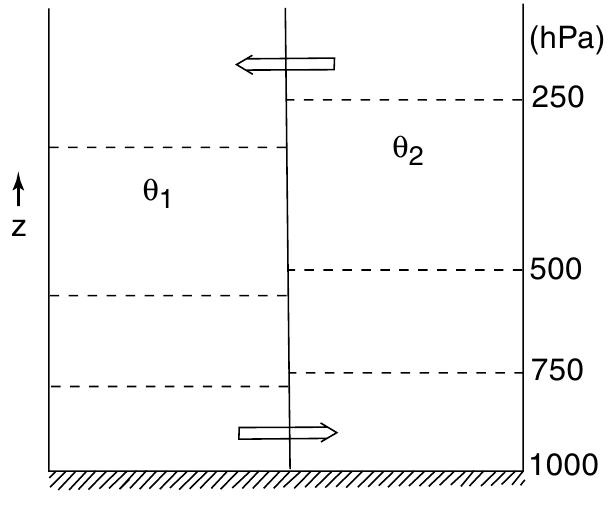
\includegraphics[scale=0.5]{{./chapters/figures_misc/holton_ape_fig}.jpeg}
\end{center}
\caption{Две воздушные массы с вертикальным разделителем. Пунктирные линии обозначают изобарические поверхности. Стрелки показывают направление движения, возникающего при удалении разделителя \citep{Holton2004}}
\label{fig:apeholton}
\end{figure}

Разность между полной потенциальной энергией и минимумом полной потенциальной энергии закрытой системы называется доступной потенциальной энергией (ДПЭ) и обозначается буквой $A$. Иначе говоря, ДПЭ есть разность между полной потенциальной энергией данного состояния атмосферы и потенциальной энергией фонового состояния. В отличие от кинетической или внутренней энергии, доступная потенциальная энергия есть интегральная характеристика и, согласно Лоренцу, пропорциональна квадрату отклонения потенциальной температуры от фонового состояния и обратно пропорциональна статической устойчивости. 

Наблюдения показывают, что лишь $0.5\%$ полной потенциальной энергии атмосферы доступно для перехода в другие виды энергии, и обычно только $10\%$ от этого количества преобразуется в кинетическую \citep{Holton2004}. С этой точки зрения атмосфера Земли является очень неэффективной тепловой машиной. 

Заметим, что перемещение масс в рассмотренном выше примере было адиабатическим. Следовательно, вывод точного выражения для ДПЭ удобно производить в изэнтропических координатах ($x,y,\theta$). При этом используем выражение для потенциальной энергии, проинтегрированное по всему расчетному объему. В данном разделе под $S$ понимается площадь, по которой производится интегрирование. Сначала запишем потенциальную энергию в изобарических координатах:
\begin{equation}
E_P=\frac{R}{g}\int_0^{p_0}dp
\end{equation}
а внутреннюю также представим через интеграл по давлению:
\begin{equation}
E_I=\frac{c_v}{g}\int_0^{p_0}Tdp
\end{equation}
Тогда полная потенциальная энергия (суммарная не только по высоте, но и по площади) будет равняться
\begin{equation}
E_T=\frac{c_p}{g}\iint_S\int_0^{p_0}TdpdS' = \frac{c_p}{g}\iint_S\int_0^{p_0}\theta\left(\frac{p}{p_{00}}\right)^\kappa dpdS' = \frac{c_p}{gp_{00}^\kappa (\kappa+1)}\iint_S\int_0^{p_0}\theta dp^{\kappa+1}dS'
\end{equation}
Это выражение путем некоторых преобразований с использованием правила интегрирования по частям и граничных условий на верхней и нижней границе атмосферы можно привести к виду
\begin{equation}
E_T=\frac{c_p}{gp_{00}^\kappa (\kappa+1)}\iint_S\int_0^{\infty}p^{\kappa+1}d\theta dS'
\end{equation}
Баротропное состояние характеризуется полной потенциальной энергией (с индексом $s$):
\begin{equation}
E_{T,s}=\frac{c_p}{gp_{00}^\kappa (\kappa+1)}\iint_S\int_0^{\infty}p_s^{\kappa+1}d\theta dS'
\end{equation}
Исходя из определения, доступная потенциальная энергия равна разности последних интегралов:
\begin{equation}
A=\frac{c_p}{gp_{00}^\kappa (\kappa+1)}\iint_S\int_0^{\infty}\left(p^{\kappa+1} - p_s^{\kappa+1}\right)d\theta dS'
\end{equation}
Пусть для давления p справедливо приближение Буссинеска
\begin{equation}
p=p_s+p', \quad p'/p_s \ll 1
\end{equation}
Тогда, если разложить подынтегральную часть выражения в степенной ряд и ограничиться двумя первыми членами разложения (причем первый из них после интегрирования исчезает), то
\begin{equation}
A=\frac{1}{2}\frac{\kappa c_p}{gp_{00}^\kappa}\iint_S\int_0^{\infty}p_s^{\kappa+1}\left(\frac{p'}{p_s}\right)^2 d\theta dS'
\end{equation}
Далее необходимо перейти обратно в изобарические координаты. Для этого принимаем
\begin{equation}
\theta - \hat{\theta}=\theta'=-\pderiv{\hat{\theta}}{p}p',
\end{equation}
что означает, что отклонение потенциальной температуры от среднего значения на изобарической поверхности пропорционально отклонению давления от его среднего на изотермической поверхности. 
Преобразовав дифференциал по формуле $d\theta=\pderiv{\theta}{p}dp$, получаем
\begin{equation}
A=-\frac{1}{2}\frac{R}{gp_{00}^\kappa}\iint_S\int_0^{p_0}p_s^{\kappa-1}\theta'^2\left(\pderiv{\hat{\theta}}{p}\right)^{-2}\pderiv{\theta}{p} dp dS'
\end{equation}
которое при равенстве $p=p_s$ на изобарической поверхности и при $\pderiv{\hat{\theta}}{p}\approx \pderiv{\theta}{p}$ преобразуется в окончательное выражение
\begin{equation} \label{eq:apeclassic}
A=-\frac{1}{2}\frac{R}{gp_{00}^\kappa}\iint_S\int_0^{p_0}p_s^{\kappa-1}\theta'^2\left(\pderiv{\hat{\theta}}{p}\right)^{-1} dp dS'
\end{equation}

\subsection{Кинетическая и доступная потенциальная энергия в уравнениях модели}
\label{sec:energymodel}
Отметим, что классическое выражение для ДПЭ \eqref{eq:apeclassic} не обязано выполняться для системы уравнений модели, которая получена при упрощениях исходной системы гидротермодинамики в z-координатах (Miranda, 1991). Поэтому ниже мы получим выражение ДПЭ, справедливое именно для модели ReMeDy, чтобы с помощью него корректно диагностировать ее результаты. Рассмотрим систему уравнений модели \eqref{eq:progn0}. Уравнения движения для трех компонент вектора скорости и уравнение притока тепла можно переписать, учитывая уравнение неразрывности \eqref{eq:progn5}, через полную производную в $\sigma$-координатах:
\begin{subequations}\label{eq:totderiv0}
\begin{align}
p_*\frac{Du}{Dt}&=-p_* \frac{\partial{\phi'}}{\partial{x}}+\sigma \frac{\partial{p_*}}{\partial{x}}\frac{\partial{\phi'}}{\partial{\sigma}}+f(v-V_g )p_*+p_*(D_u+R_u )\label{eq:totderiv1} \\
p_*\frac{Dv}{Dt}&=-p_* \frac{\partial{\phi'}}{\partial{y}}+\sigma \frac{\partial{p_*}}{\partial{y}}\frac{\partial{\phi'}}{\partial{\sigma}}-f(u-U_g )p_*+p_*(D_v+R_v )\label{eq:totderiv2} \\
p_*\frac{D\tilde{w}}{Dt}&=S_vp_* \frac{\partial{\phi'}}{\partial{\sigma}}+p_*g\frac{\theta'}{\theta_S}+p_*(D_{\tilde{w}}+R_{\tilde{w}})\label{eq:totderiv3} \\
p_*\frac{D\theta'}{Dt}&=S_v\tilde{w}p_*\frac{\partial{\theta_s}}{\partial{\sigma}}+p_*Q+p_*(D_{\theta}+R_{\theta}),\label{eq:totderiv4} 
\end{align}
\end{subequations}
где $\frac{D}{Dt}=\frac{\partial}{\partial{t}} +u \frac{\partial}{\partial{x}}+ v\frac{\partial}{\partial{y}}+ \dot{\sigma}\frac{\partial}{\partial{\sigma}}$.

\subsection{Бюджет полной кинетической энергии}
Известно, что удельная кинетическая энергия частицы $E_k$ пропорциональна сумме квадратов скорости:
$$E_k=\frac{1}{2}\left(u^2+v^2+\tilde{w}^2\right).$$
Уравнение для эволюции кинетической энергии получим, умножив каждое уравнение движения \eqref{eq:totderiv1}--\eqref{eq:totderiv3} на соответствующую компоненту вектора скорости и сложив полученные выражения:
\begin{subequations}\label{eq:ek0}
\begin{align}
\frac{1}{2}p_*\frac{Du^2}{Dt}&=-p_*u \frac{\partial{\phi'}}{\partial{x}}+\sigma u \frac{\partial{p_*}}{\partial{x}}\frac{\partial{\phi'}}{\partial{\sigma}}+f(v-V_g )p_*u+p_*u(D_u+R_u )\label{eq:ek1} \\
\frac{1}{2}p_*\frac{Dv^2}{Dt}&=-p_*v \frac{\partial{\phi'}}{\partial{y}}+\sigma v \frac{\partial{p_*}}{\partial{y}}\frac{\partial{\phi'}}{\partial{\sigma}}-f(u-U_g )p_*v+p_*v(D_v+R_v )\label{eq:ek2} \\
\frac{1}{2}p_*\frac{D\tilde{w}^2}{Dt}&=S_vp_*\tilde{w}\frac{\partial{\phi'}}{\partial{\sigma}}+p_*g\tilde{w}\frac{\theta'}{\theta_S}+p_*\tilde{w}(D_{\tilde{w}}+R_{\tilde{w}})\label{eq:ek3} \\
p_*\frac{DE_k}{Dt}&=-p_*u \pderiv{\phi'}{x}-p_*v \pderiv{\phi'}{y}+\sigma u \pderiv{p_*}{x}\pderiv{\phi'}{\sigma}+\sigma v \pderiv{p_*}{y}\pderiv{\phi'}{\sigma}+S_vp_*\tilde{w}\pderiv{\phi'}{\sigma}+\nonumber \\ 
&+p_*g\tilde{w}\frac{\theta'}{\theta_S}+fp_*(vU_g-uV_g) + \mathcal{D}_{u,v,w}, \label{eq:ek4}
\end{align}
\end{subequations}
где $\mathcal{D}_{u,v,w}$ обозначает сумму слагаемых, ответственных за турбулентную вязкость, пространственные и временные фильтры, приводящие к диссипации КЭ.

Первые пять слагаемых в правой части \eqref{eq:ek4} могут быть переписаны в более удобной форме (компоненты геострофической скорости опущены):
\begin{align}
 &-p_*u \pderiv{\phi'}{x}-p_*v \pderiv{\phi'}{y}+\sigma u \pderiv{p_*}{x}\pderiv{\phi'}{\sigma}+\sigma v \pderiv{p_*}{y}\pderiv{\phi'}{\sigma}+S_vp_*\tilde{w}\pderiv{\phi'}{\sigma}= \nonumber \\
=&-p_*u \pderiv{\phi'}{x}-p_*v \pderiv{\phi'}{y}+\sigma\pderiv{\phi'}{\sigma}\left(u\pderiv{p_*}{x}+ v\pderiv{p_*}{y}\right)-(p_*\dot{\sigma}+\sigma\dot{p_*})\pderiv{\phi'}{\sigma}= \nonumber \\
=&-p_*u \pderiv{\phi'}{x}-p_*v \pderiv{\phi'}{y}+\sigma\pderiv{\phi'}{\sigma}\left(u\pderiv{p_*}{x}+v\pderiv{p_*}{y}\right)-\sigma\pderiv{\phi'}{\sigma}\frac{Dp_*}{Dt}-p_*\dot{\sigma}\pderiv{\phi'}{\sigma}=\nonumber\\
=&-p_*u \pderiv{\phi'}{x}-p_*v \pderiv{\phi'}{y}-\sigma\pderiv{\phi'}{\sigma}\pderiv{p_*}{t}-p_*\dot{\sigma}\pderiv{\phi'}{\sigma}=\nonumber\\
=&-p_*u \pderiv{\phi'}{x}-p_*v \pderiv{\phi'}{y}-\phi'\left(u\pderiv{p_*}{x}+v\pderiv{p_*}{y}\right)-p_*\dot{\sigma}\pderiv{\phi'}{\sigma}+\phi'\left(u\pderiv{p_*}{x}+v\pderiv{p_*}{y}\right)+\phi'\pderiv{p_*}{t}-\phi'\pderiv{p_*}{t}-\sigma\pderiv{\phi'}{\sigma}\pderiv{p_*}{t}=\nonumber\\
=&-p_*u \pderiv{\phi'}{x}-p_*v \pderiv{\phi'}{y}-\phi'\left(u\pderiv{p_*}{x}+v\pderiv{p_*}{y}\right)-p_*\dot{\sigma}\pderiv{\phi'}{\sigma}+\phi'\frac{Dp_*}{Dt}-\phi'\pderiv{p_*}{t}-\sigma\pderiv{\phi'}{\sigma}\pderiv{p_*}{t}=\nonumber\\
=&-u \pderiv{p_*\phi'}{x}-v \pderiv{p_*\phi'}{y}-p_*\dot{\sigma}\pderiv{\phi'}{\sigma}+\phi'\frac{Dp_*}{Dt}-\pderiv{p_*}{t}\pderiv{(\sigma\phi')}{\sigma}=\nonumber\\
=&-u \pderiv{p_*\phi'}{x}-v \pderiv{p_*\phi'}{y}-\dot{\sigma}\pderiv{p_*\phi'}{\sigma}-\phi'p_*\left(\pderiv{u}{x}+\pderiv{v}{y}+\pderiv{\dot{\sigma}}{\sigma}\right)-\pderiv{p_*}{t}\pderiv{(\sigma\phi')}{\sigma}=\nonumber\\
=&-\pderiv{p_*u\phi'}{x}-\pderiv{p_*v\phi'}{y}-\pderiv{p_*\dot{\sigma}\phi'}{\sigma}-\pderiv{p_*}{t}\pderiv{(\sigma\phi')}{\sigma}.
\end{align}

После этих преобразований выражение для кинетической энергии можно переписать в дивергентной форме:
\begin{subequations}
\begin{align}
p_*\frac{DE_k}{Dt}&=-\pderiv{p_*u\phi'}{x}-\pderiv{p_*v\phi'}{y}-\pderiv{p_*\dot{\sigma}\phi'}{\sigma}-\pderiv{p_*}{t}\pderiv{\sigma\phi'}{\sigma}+p_*g\tilde{w}\frac{\theta'}{\theta_S}-fp_*(V_gu-U_gv) + \mathcal{D}_{u,v,w}, \\
\intertext{или} \nonumber \\
\frac{\partial{p_*E_k}}{\partial{t}}&=-\frac{\partial{p_*uE_k}}{\partial{x}}-\frac{\partial{p_*vE_k}}{\partial{y}}-\frac{\partial{p_*\dot{\sigma}E_k}}{\partial{\sigma}}-\frac{\partial{p_*u\phi'}}{\partial{x}}-\frac{\partial{p_*v\phi'}}{\partial{y}}-\frac{\partial{p_*\dot{\sigma}\phi'}}{\partial{\sigma}}+ \nonumber \\ 
&-\pderiv{p_*}{t}\pderiv{\sigma\phi'}{\sigma}+p_*g\tilde{w}\frac{\theta'}{\theta_S}-fp_*(V_gu-U_gv) + \mathcal{D}_{u,v,w} \label{eq:ektend}.
\end{align}
\end{subequations}

\subsection{Бюджет доступной энергии}
Чтобы получить аналогичное уравнение для доступной потенциальной энергии (ДПЭ), сначала умножим уравнение \eqref{eq:totderiv4} на возмущение потенциальной температуры $\theta'$:
\begin{align}
\frac{1}{2}p_*\frac{D\theta'^2}{Dt}&=S_v\tilde{w}p_*\theta'\frac{\partial{\theta_s}}{\partial{\sigma}}+p_*\theta'Q+p_*\theta'(D_{\theta}+R_{\theta}) \label{eq:th2}.
\end{align}

Как было показано в предыдущем разделе, ДПЭ пропорциональна квадрату отклонения потенциальной температуры от фонового состояния, деленной на статическую устойчивость. В системе координат модели ReMeDy статическая устойчивость, или квадрат частоты Брента-Вяйсяля, записывается следующим образом 
\begin{equation}
N^2=-S_v\frac{g}{\theta_s}\frac{\partial\theta_s}{\partial\sigma}. \label{eq:bfreq}
\end{equation}

Тогда разделим \eqref{eq:th2} на $N^2$ и умножим его на $\left(\frac{g}{\theta_s}\right)^2$. Другими словами, умножим уравнение притока тепла на величину, обратную градиенту температуры, обозначив ее $B^2$:
\begin{subequations}
\begin{align}
\frac{1}{2}p_*B^2\frac{D\theta'^2}{Dt}&=-gp_*\tilde{w}\frac{\theta'}{\theta_s}+p_*\theta'B^2Q+p_*\theta'B^2(D_{\theta}+R_{\theta})
\intertext{где}
B^2&=\left(\frac{g}{\theta_s}\right)^2N^{-2}=-\frac{g/\theta_s}{S_v \partial\theta_s/\partial\sigma}=\frac{g/\theta_s}{ \partial\theta_s/\partial{z}} \label{eq:B2}.
\end{align}
\end{subequations}

Используя правило дифференцирования произведения и уравнение неразрывности \eqref{eq:progn5}, можно записать
\begin{align}
\frac{1}{2}p_*\frac{D\theta'^2B^2}{Dt}&=\frac{1}{2}\left(\frac{\partial{p_*\theta'^2B^2}}{\partial{t}}+\frac{\partial{p_*u\theta'^2B^2}}{\partial{x}}+\frac{\partial{p_*v\theta'^2B^2}}{\partial{y}}+\frac{\partial{p_*\dot{\sigma}\theta'^2B^2}}{\partial{\sigma}}\right)= \nonumber\\ 
&=-gp_*\tilde{w}\frac{\theta'}{\theta_s}+\frac{1}{2}p_*\theta'^2\frac{DB^2}{Dt}+p_*\theta'B^2Q+p_*\theta'B^2(\mathcal{D}_{\theta}+R_{\theta}) \label{eq:apetend}
\end{align}
где $\theta'^2B^2$ может быть интерпретировано как ДПЭ на единицу массы. Под знаком полной производной находится выражение, которое есть доступная потенциальная энергия. Если сравнить \eqref{eq:ektend} и \eqref{eq:apetend2}, становится видно, что слагаемое $gp_*\tilde{w}\frac{\theta'}{\theta_s}$, которое присутствует в обоих уравнениях, но с разными знаками, можно интерпретировать как переход энергии из доступной потенциальной в кинетическую и обратно.

Согласно \eqref{eq:B2}, параметр $B^2$ зависит только от вертикальной координаты. Следовательно, полная производная, входящая во второе слагаемое в правой части уравнения \eqref{eq:apetend}, после нескольких преобразований превращается в следующее выражение
\begin{align}
\frac{DB^2}{Dt}=\frac{\partial{B^2}}{\partial{t}}+u \frac{\partial{B^2}}{\partial{x}}+v\frac{\partial{B^2}}{\partial{y}}+\tilde{w}\frac{\partial{B^2}}{\partial{z}} \approx \tilde{w}\frac{\partial{B^2}}{\partial{z}}=-\frac{g\tilde{w}}{\theta_s}\left(\frac{\partial\theta_s}{\partial{z}}\right)^{-2}\left(\frac{Dln\theta_s}{Dz}-\frac{D^2\theta_s}{Dz^2}\right) \label{eq:dB2}.
\end{align}
Отметим, что если фоновое изменение потенциальной температуры задано линейной функцией, то вычитаемое, стоящее в скобках \eqref{eq:dB2}, становится равным нулю. В данной работе профиль $\theta_s$ являлся именно линейным, так что 
\begin{equation}
B^2=-\frac{g\tilde{w}}{\theta_s^2}\left(\frac{\partial\theta_s}{\partial{z}}\right)^{-1}
\end{equation}
Значит, тенденцию ДПЭ на единицу массы, $E_a=\frac{1}{2}\theta'^2B^2$, можно переписать в виде
\begin{align}
\frac{\partial p_*E_a}{\partial{t}}&=-\frac{\partial{p_*uE_a}}{\partial{x}}-\frac{\partial{p_*vE_a}}{\partial{y}}-\frac{\partial{p_*\dot{\sigma}E_a}}{\partial{\sigma}} \nonumber\\ 
&=-gp_*\tilde{w}\frac{\theta'}{\theta_s}-\frac{1}{2}gp_*\tilde{w}\left(\frac{\theta'}{\theta_s}\right)^2\left(\frac{\partial\theta_s}{\partial{z}}\right)^{-1}p_*\theta'B^2(Q+\mathcal{D}_\theta) \label{eq:apetend2}.
\end{align} %%+gp_*\frac{\theta'}{\theta_s}\frac{1}{ \partial\theta_s/\partial{z}}\frac{L_v}{c_p}\left(\frac{p_0}{p}\right)^{R_d/c_p}(C-E)

Доступная потенциальная энергия, как было показано в разделе \ref{sec:APEtheory}, есть интегральная величина. Принимая во внимание верхнее и нижнее граничные условия ($\dot{\sigma}_{\sigma=0,1}=0$), получаем интегральную форму уравнений \eqref{eq:apetend2} и \eqref{eq:ektend}. Так, изменение полной (интегральной) кинетической энергии $K=\frac{1}{g}\iiint\limits_V p_*E_k dxdyd\sigma$ во времени равно:
\begin{align} \label{eq:dKdt}
\frac{d}{dt}K&=\frac{1}{g}\iint\left[(p_*uE_k)_{x=x_1}-(p_*uE_k)_{x=x_2}\right]dyd\sigma + \frac{1}{g}\iint\left[(p_*vE_k)_{y=y_1}-(p_*vE_k)_{y=y_2}\right]dxd\sigma + \nonumber\\ &+\frac{1}{g}\iint\left[(p_*u\phi^\prime)_{x=x_1}-(p_*u\phi^\prime)_{x=x_2}\right]dyd\sigma + \frac{1}{g}\iint\left[(p_*v\phi^\prime)_{y=y_1}-(p_*v\phi^\prime)_{y=y_2}\right] dxd\sigma + \nonumber\\ &+ \iiint p_*\tilde{w}\frac{\theta^\prime}{\theta_s}dxdyd\sigma - \frac{1}{g}\iiint p_*f(V_gu-U_gv) dxdyd\sigma+\frac{1}{g}\iiint \mathcal{D}_{u,v,w}dxdyd\sigma
\end{align}
а изменение ДПЭ, $A=\frac{1}{g}\iiint\limits_V p_*E_a dxdyd\sigma$ равно:
\begin{align} \label{eq:dAdt}
\frac{d}{dt}A&=\frac{1}{g}\iint\left[(p_*uE_a)_{x=x_1}-(p_*uE_a)_{x=x_2}\right]dyd\sigma + \frac{1}{g}\iint\left[(p_*vE_a)_{y=y_1}-(p_*vE_a)_{y=y_2}\right]dxd\sigma - \nonumber\\ &- \iiint p_*\tilde{w}\frac{\theta^\prime}{\theta_s}dxdyd\sigma \nonumber\\
&+ \frac{1}{2}\iiint p_*\tilde{w}\left(\frac{\theta^\prime}{\theta_s}\right)^2\left(\frac{\partial\theta_s}{\partial z}\right)^{-1}dxdyd\sigma+\frac{1}{g}\iiint p_*\theta'B^2Qdxdyd\sigma+\frac{1}{g}\iiint p_*\theta'B^2\mathcal{D}_{\theta}dxdyd\sigma.
\end{align} %+\iiint \left(p_*\frac{\theta'}{\theta_s}\frac{1}{ \partial\theta_s/\partial{z}}\frac{L_v}{c_p}\left(\frac{p_0}{p}\right)^{R_d/c_p}(C-E)\right) dxdyd\sigma

\subsubsection{Потоки тепла с поверхности}
\label{sec:expsetup:hsurf}
Вернемся к выражению \eqref{eq:apetend}. Заметим, что первое слагаемое в скобках отвечает за подсеточное турбулентное перемешивание, и в модели определяется через коэффициент турбулентной теплопроводности (для замыкания Смагоринского-Лилли, см. раздел \ref{sec:model:closure}.

Термическая диффузия в нашей работе представлялась только вертикальной ее компонентой, так что для простоты следующие выкладки будут включать пространственные производные только для $\sigma$:
\begin{equation}
D_\theta=S_v\pderiv{}{\sigma}K_H S_v\pderiv{\theta}{\sigma}
\end{equation}

Интегрирование этого выражения по высоте и использование правила интегрирования по частям дает
\begin{align}
\int_\sigma p_*\theta'B^2S_v\pderiv{}{\sigma}\left(K_H S_v\pderiv{\theta}{\sigma}\right)d\sigma&=\left(p_*\theta'B^2S_v^2K_H \pderiv{\theta}{\sigma}\right)_{\sigma=0}-\left(p_*\theta'B^2S_v^2K_H \pderiv{\theta}{\sigma}\right)_{\sigma=1} \\ 
&-\int_\sigma p_*\pderiv{\theta'S_vB^2}{\sigma}S_vK_H\pderiv{\theta}{\sigma}d\sigma \label{eq:subgrid_mixing_theta}
\end{align}
Первое слагаемое в правой части уравнения выше включает поток тепла на верхней границе области, который в силу граничных условий равен нулю, в то время как второе слагаемое определяется нижним граничным условием, которое зависит от потока тепла с поверхности ($H_{surf}=-K_H S_v\pderiv{\theta}{\sigma}c_p\rho\left(\frac{p}{p_0}\right)^{\kappa}$). Последний член в \eqref{eq:subgrid_mixing_theta} может быть интерпретирован как диссипация ДПЭ через теплопроводность. В результате этих преобразований ур. \eqref{eq:subgrid_mixing_theta} принимает вид:
\begin{equation}
\int_\sigma\theta'B^2\mathcal{D}_\theta d\sigma=\left(\theta'B^2S_v\right)_{\sigma=1}\frac{H_{surf}}{c_p\rho}\left(\frac{p_0}{p}\right)^{\kappa}-\int_\sigma \pderiv{\theta'S_vB^2}{\sigma}S_vK_H\pderiv{\theta}{\sigma}d\sigma \label{eq:subgrid_mixing_theta_fin}
\end{equation}

\begin{thebibliography}{12}
 \bibitem{ER89}
Emanuel KA, Rotunno R. 1989. Polar lows as Arctic hurricanes. \textit{Tellus} \textbf{41A:} 1-17.
\end{thebibliography}

\end{document}
\documentclass[12pt,a4paper]{report}

%
% PACKAGES AND STYLES
%

% 
% Language and encoding
%
%\usepackage{mathtext}
%\usepackage[T2A]{fontenc}
\usepackage[utf8]{inputenc}
\usepackage[english,russian]{babel}
\usepackage{mmap}

%
% Colors
%
\usepackage[usenames]{color}
\usepackage{color}
\usepackage{colortbl}

%
% Symbols
%
\usepackage{amssymb}
\usepackage{MnSymbol}

%
% Units
%
%\usepackage[binary-units=true]{siunitx}
\newcommand{\km}{\mathrm{~\text{км}}}
\newcommand{\m}{\mathrm{~\text{м}}}
\newcommand{\s}{\mathrm{~\text{с}}}
\newcommand{\mps}{\m \s ^{-1}}
\newcommand{\pers}{\s ^{-1}}
\newcommand{\K}{\mathrm{~\text{К}}}
\newcommand{\Kpkm}{\K\km ^{-1}}
\newcommand{\hpa}{\mathrm{~\text{гПа}}}
\newcommand{\J}{\mathrm{~\text{Дж}}}
\newcommand{\Jpm}{\J \m ^{-3}}

%
% Paper size and margins
%
\usepackage{vmargin}
\setmarginsrb{2.5cm}{1cm}{2.5cm}{2cm}{0cm}{0cm}{0cm}{1.5cm}

%
% Page style
%
\usepackage{fancyhdr}
\setlength{\headheight}{16pt}
\newcommand{\changefont}{%
    \fontsize{9}{11}\selectfont
}
\fancyhf{}
\fancyhead[RO]{\changefont \slshape \rightmark} %section
\fancyhead[LO]{\changefont \slshape \leftmark} %chapter
\fancyfoot[C]{\changefont \thepage} %footer
\setlength{\headsep}{0.2in}
\pagestyle{fancy}

%
% Indenting
%
\usepackage{indentfirst}
\setlength{\parindent}{1cm}
\setlength{\parskip}{0.5cm}

%
% References
%
\usepackage{natbib}

%
% Hyperlinks
%
\usepackage[linktocpage=true,plainpages=false,pdfpagelabels=false]{hyperref}
\definecolor{linkcolor}{rgb}{0.1,0,0.9}
\definecolor{citecolor}{rgb}{0,0,0.9}
\definecolor{urlcolor}{rgb}{0,0,1}
\hypersetup{
    colorlinks, linkcolor={linkcolor},
    citecolor={citecolor}, urlcolor={urlcolor}
}

\bibliographystyle{plainnat}
% Bibliography: set article volume number in bold font
%\DeclareFieldFormat
%  [article]
%  {volume}{\textbf{#1}}
%\renewcommand\nameyeardelim{, }

%\usepackage{showkeys} % show labels

\newcommand{\figref}[1]{\mbox{Figure~\ref{#1}}}
\newcommand{\tabref}[1]{\mbox{Table~\ref{#1}}}
\newcommand{\secref}[1]{\mbox{Section~\ref{#1}}}
\newcommand{\chpref}[1]{\mbox{Chapter~\ref{#1}}}
\newcommand{\appref}[1]{\mbox{Appendix~\ref{#1}}}
\newcommand{\eqnref}[1]{\mbox{Eq.~(\ref{#1})}}
\newcommand{\listref}[1]{\mbox{Listing~(\ref{#1})}}

%
% Lists
%
\usepackage[shortlabels]{enumitem}

\newenvironment{sqlist}[1][\enskip$\filledsquare$]
        {\begin{itemize}[#1]}
        {\end{itemize}}

% New math commands
% differential d, from http://tex.stackexchange.com/a/60546/586
\newcommand*\diff{\mathop{}\!\mathrm{d}}
\newcommand\mean[1]{\overline{#1}}
\newcommand{\PDt}[2]{\partial #1/\partial #2}

%
% Tables
%
\usepackage{booktabs}
%\usepackage{tabularx}
\usepackage{tabu}
\usepackage{longtable}

%
% Figures
%
\usepackage{wrapfig}
\usepackage[font=small,textfont=it,labelfont=bf]{caption}
%\captionsetup[figure]{labelfont=bf}
\usepackage{tikz}
\usepackage{pgfplots}
\usetikzlibrary{calc}

%
% Equations
%
\usepackage{cool}


\begin{document}
\setcounter{chapter}{3}
\chapter{Результаты}
Данный раздел посвящен обзору результатов численного моделирования, постановка которых описана выше. Раздел построен следующим образом: сначала рассматривается контрольный эксперимент, а именно структура, динамика и энергетика вихря. Затем аналогичным образом описывается эксперимент со включенной параметризацией микрофизики, и оценивается чувствительность вихря к начальному содержанию влаги в атмосфере.

\begin{wrapfigure}{L}{0.5\textwidth}
\begin{center}
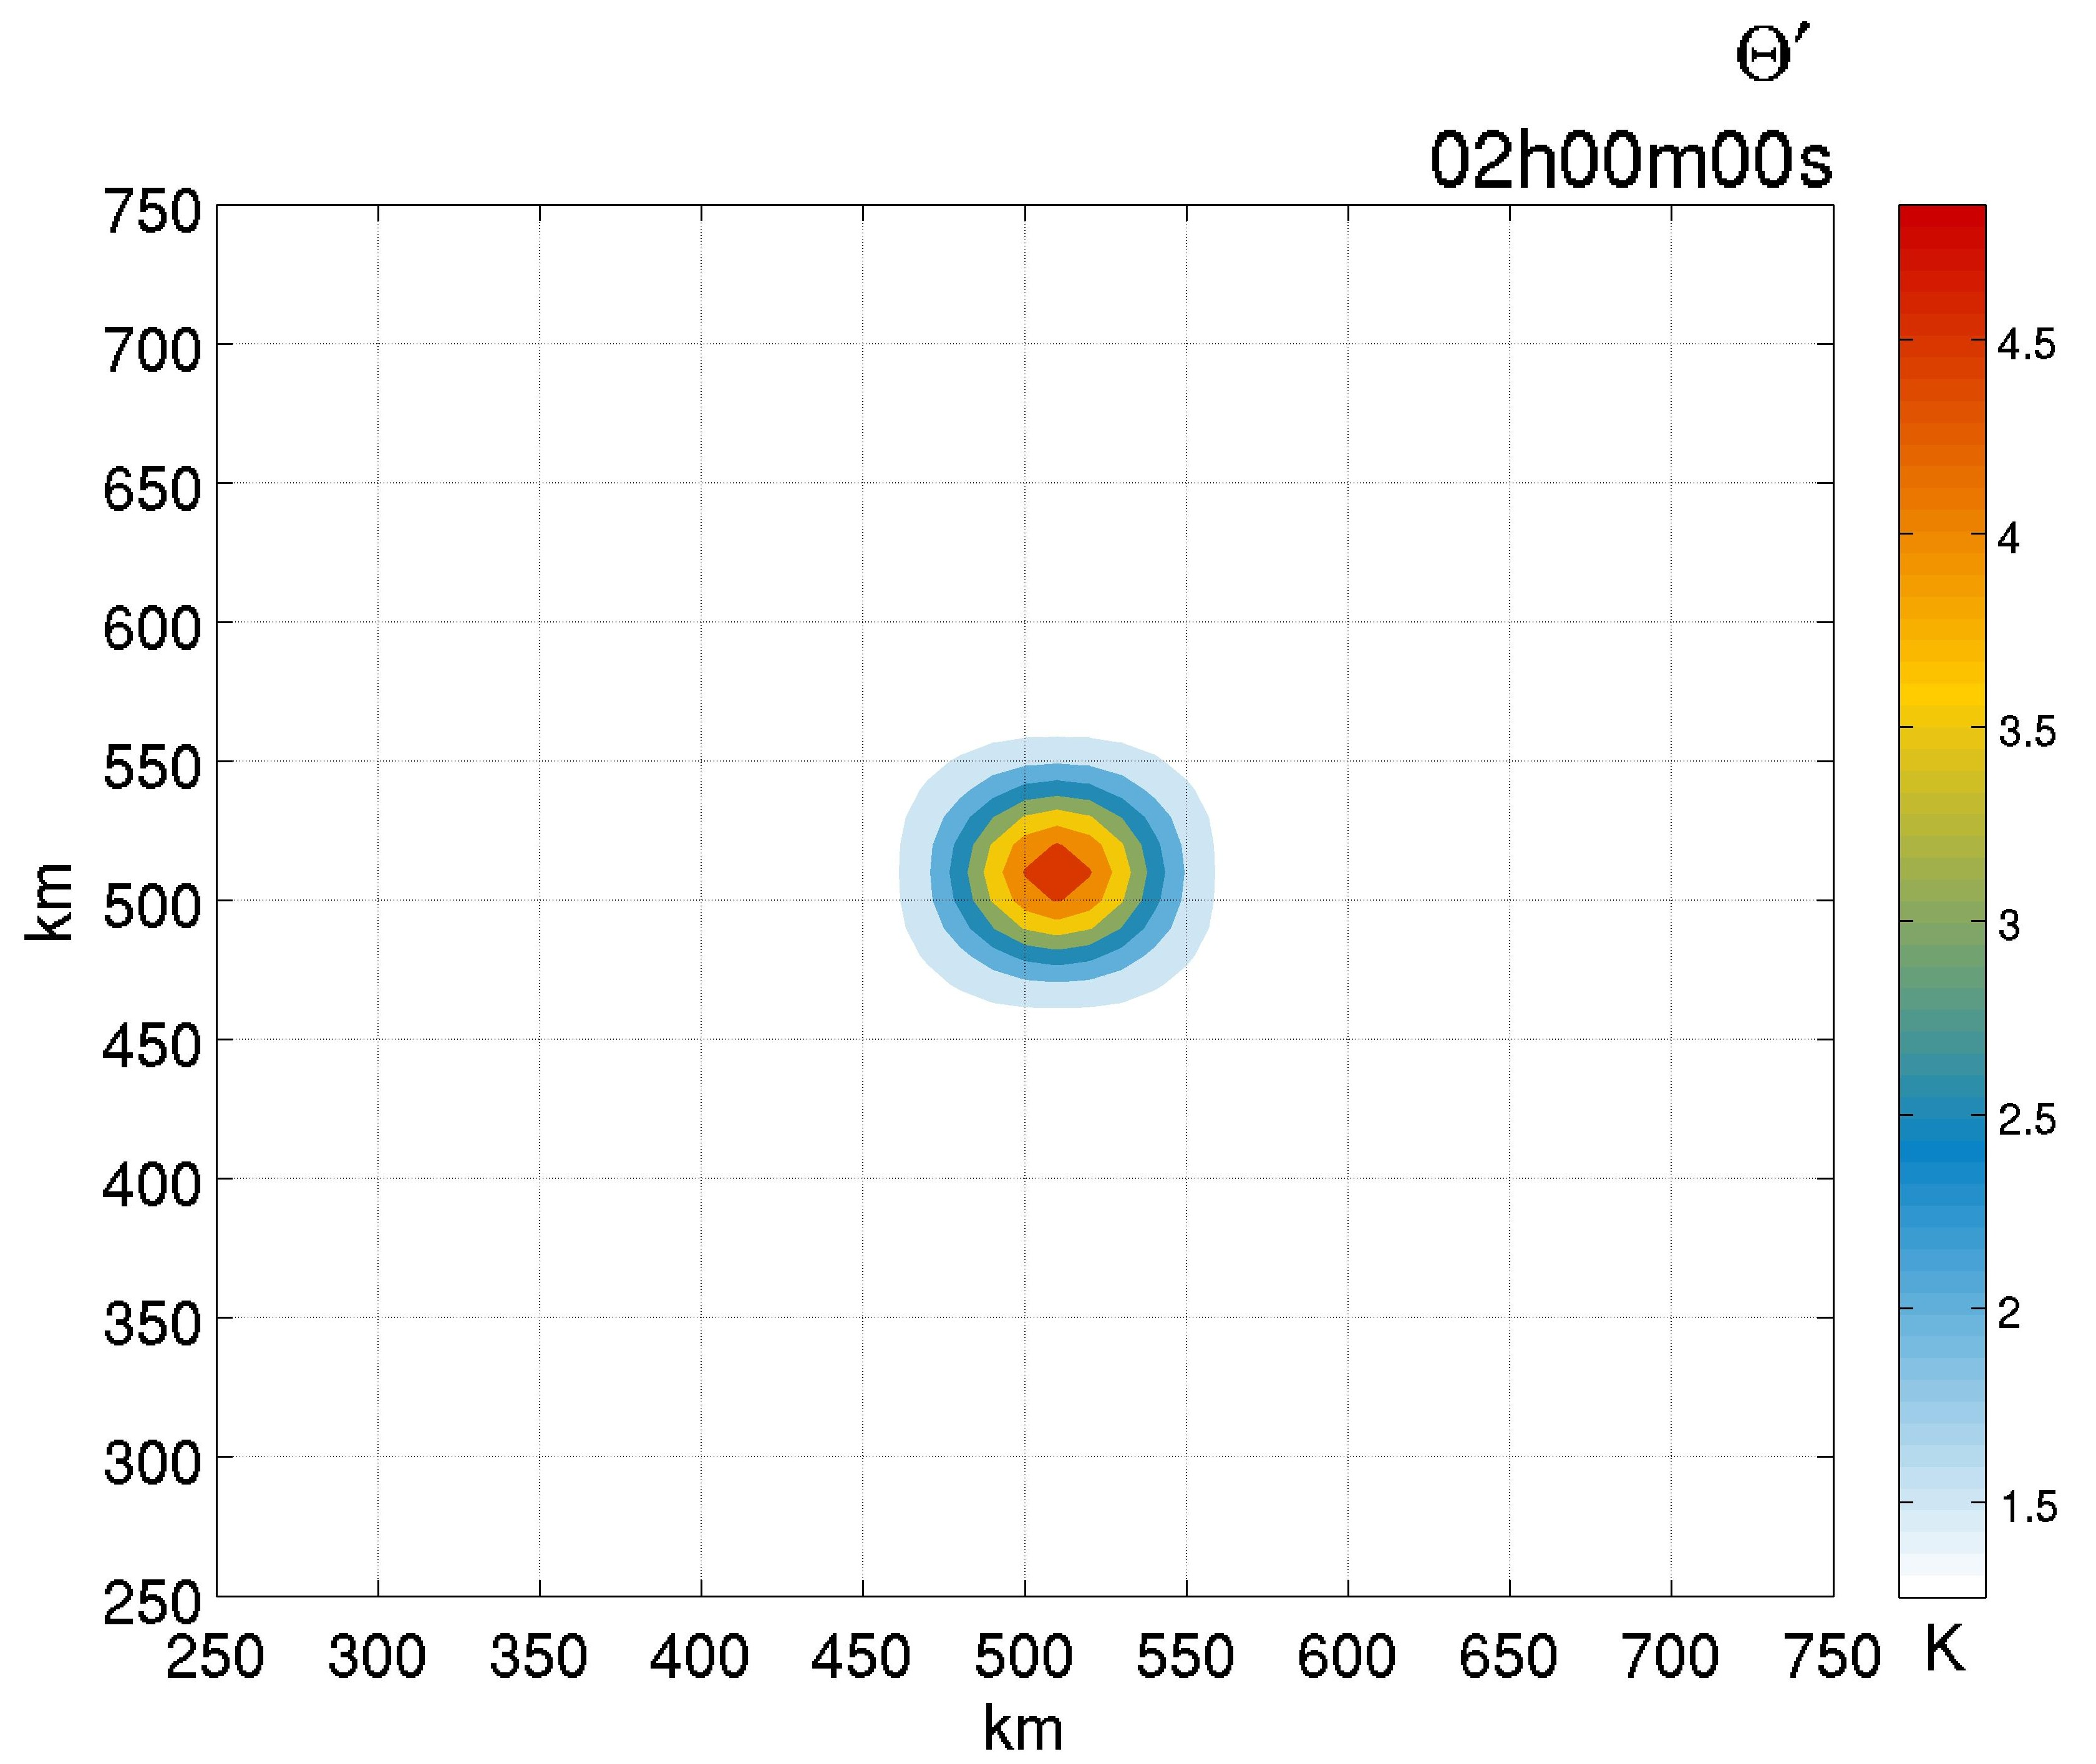
\includegraphics[width=\linewidth]{{./chapters/figures_results/ctrl_fields/pt_dev_z.x26-x76.y26-y76.ilev01.020000}.jpg}
\end{center}
\caption{Поле отклонений температуры ($\theta'$) при инициализации возмущения (2 ч. модельного времени)}
\label{fig:initanom}
\end{wrapfigure}

Влияние остальных факторов на динамику мезоциклона рассматривается с точки зрения таких интегральных характеристик, как кинетическая энергия, максимальная завихренность, минимальное приземное давление. Для интерпретации различий в результатах оценочных экспериментов привлекается анализ пространственной структуры метеополей.

Полярный мезоциклон в каждом эксперименте развивался с разной скоростью, и продолжительность экспериментов составляет 1--3 сут. Трехмерные поля в каждый момент времени интерполируются на регулярную сетку с горизонтальным разрешением, соответствующим разрешению модели. В экспериментах без фонового потока горизонтальные разрезы сфокусированы на район развития вихря (обычно $200\times 200\km$ в центре области). По вертикали данные интерполируются на регулярную сетку с шагом $500\m$ для удобства последующего постпроцессинга. В некоторых экспериментах также используется интерполяция на изобарические поверхности от $1000$ до $250\hpa$ с шагом $50\hpa$.

\section{Контрольный эксперимент}
\subsection{Начальная стадия развития вихря}
Начнем с рассмотрения момента инициализации температурной аномалии. Ее форма и начальная амплитуда видна на рис. \ref{fig:initanom}.

\begin{wrapfigure}{R}{0.5\textwidth}
\begin{center}
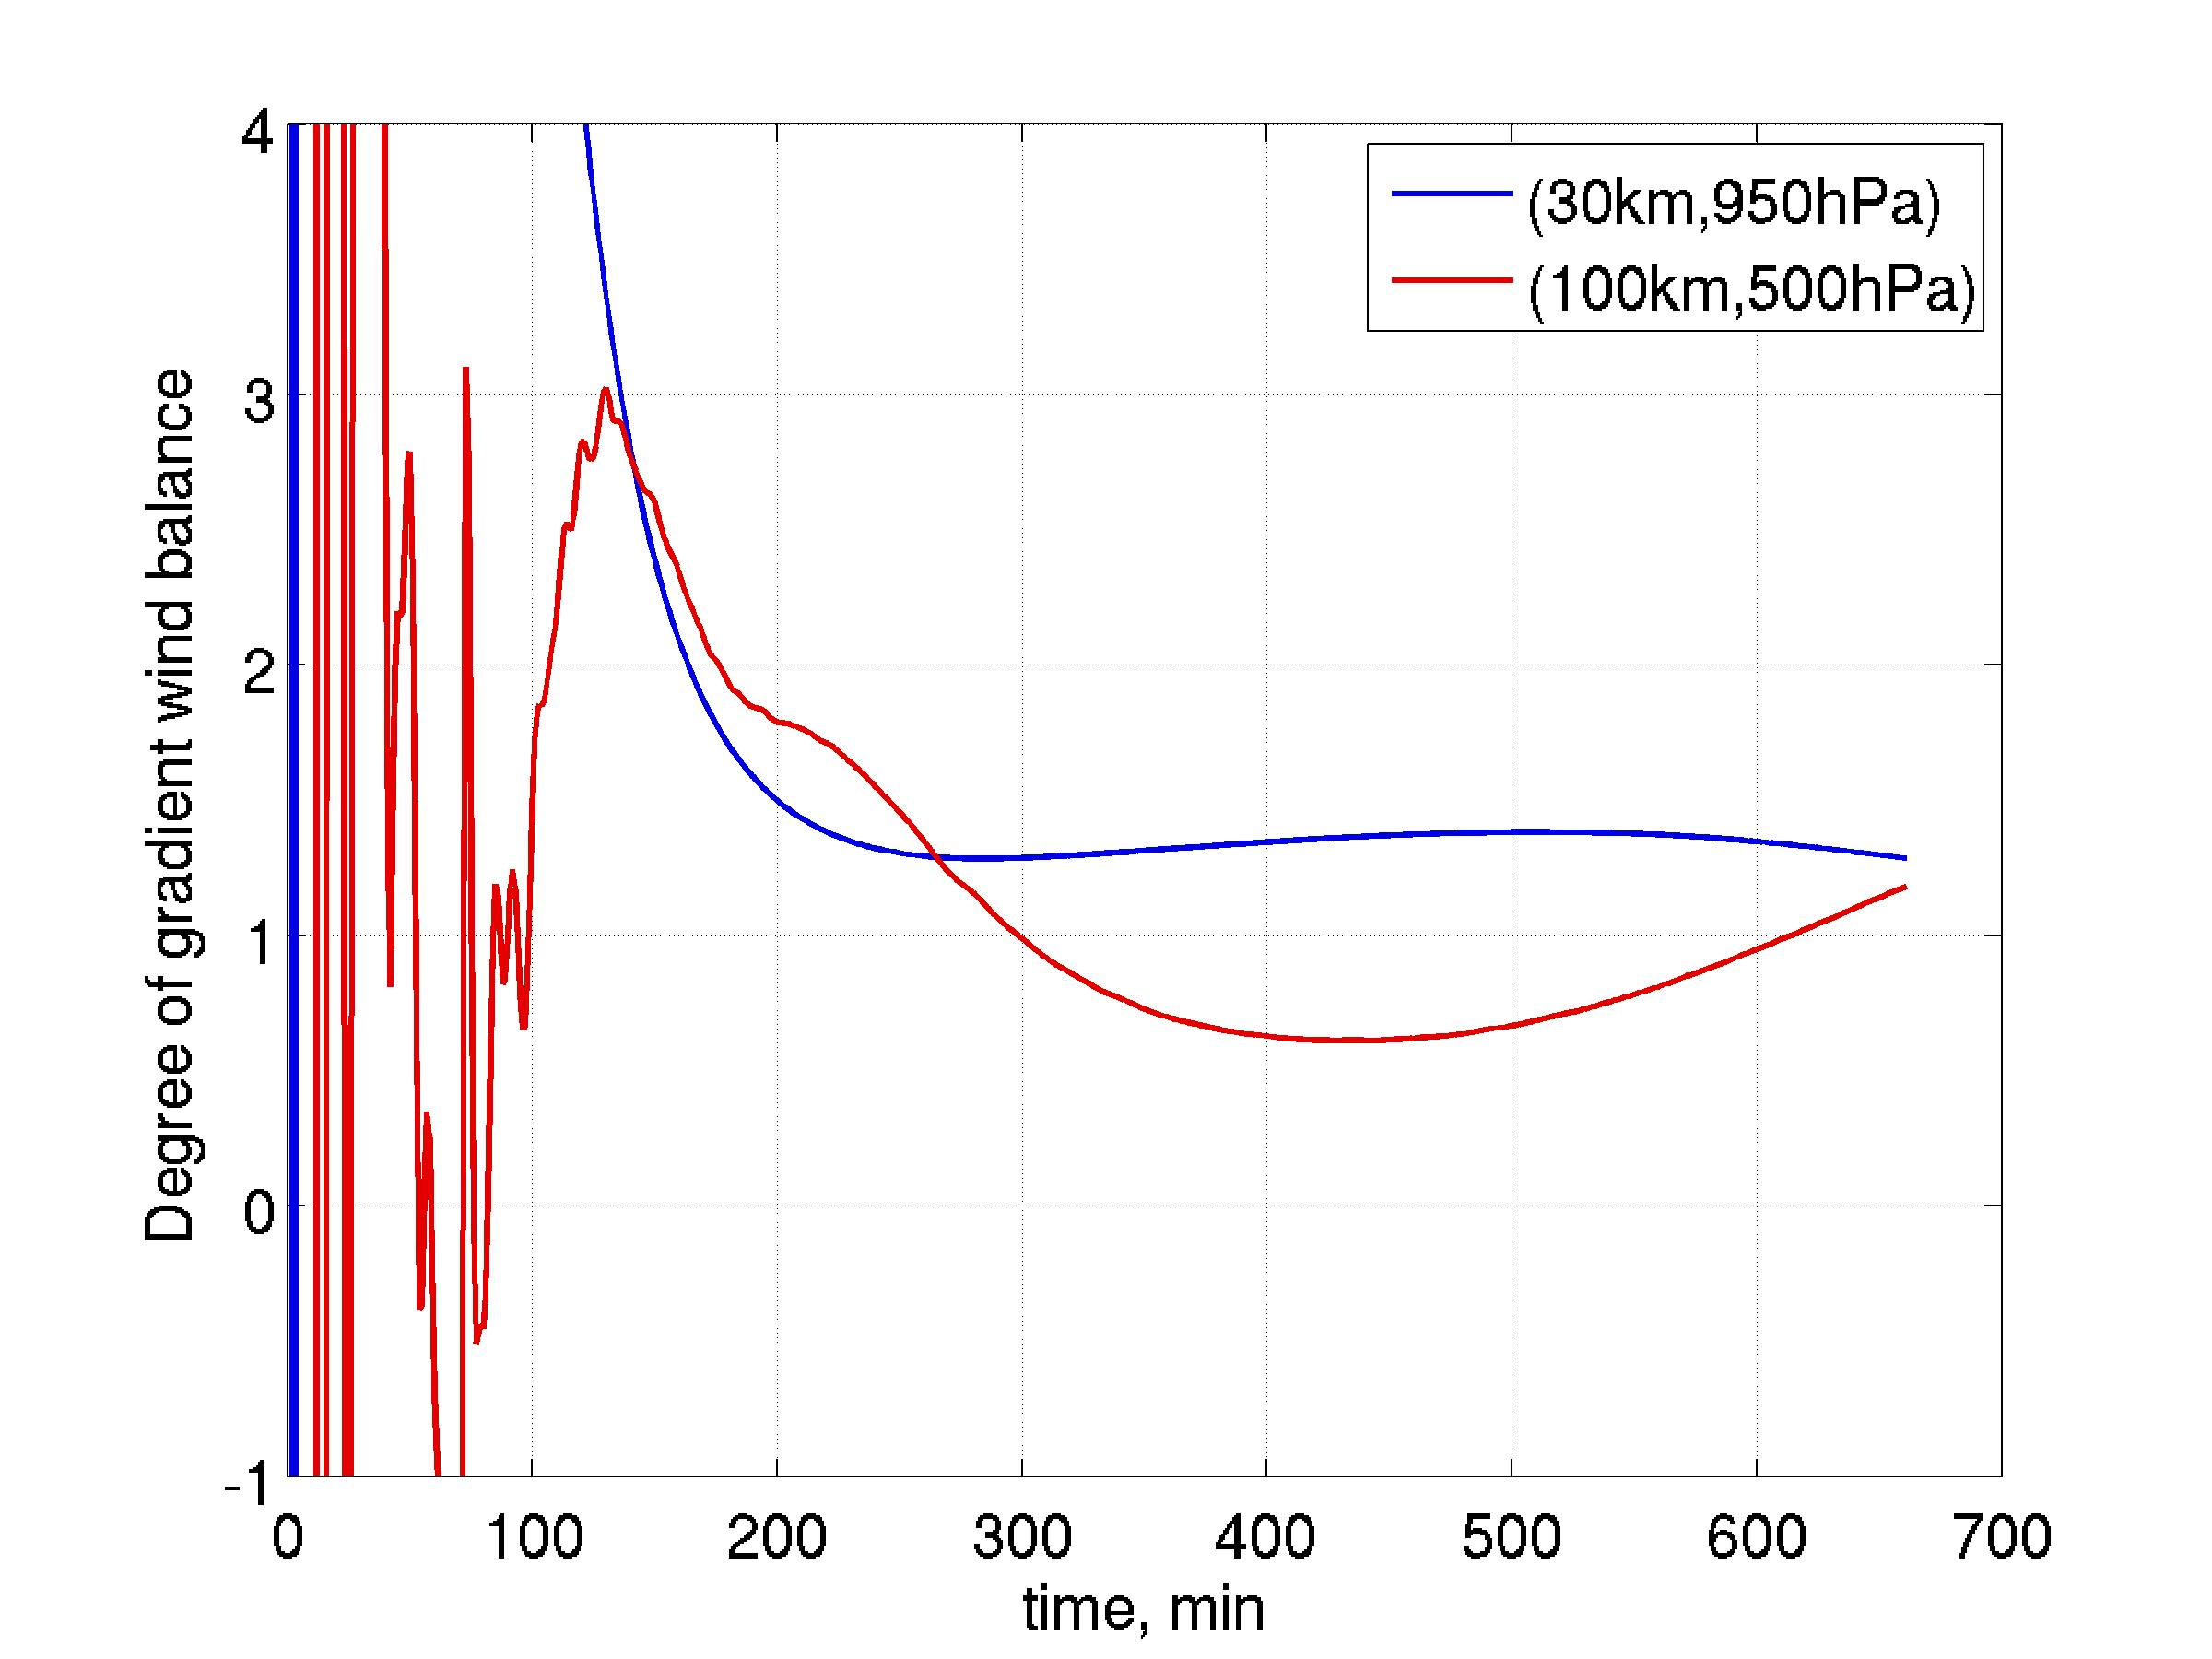
\includegraphics[width=\linewidth]{{./chapters/figures_results/ctrl_grwindbal2p}.jpg}
\end{center}
\caption{Величина градиентного баланса $\pderiv{\phi'}{r}/\left(v^2_t/r+fv_t\right)$ как функция времени с момента инициализации возмущения: при $r=30\km, p=950\hpa$ (синяя кривая) и при $r=100\km, p=500\hpa$ (красная кривая). Градиентный баланс достигается, когда кривые приближаются к $1$.}
\label{fig:grwindbal}
\end{wrapfigure} 

Появление источника тепла в атмосфере, находящейся в равновесии, ставит проблему реакции атмосферы и достижения нового баланса через механизм приспособления. Этот вопрос впервые был развит Лэмбом \citep{RT2003}, который изучал особенности волн, излучаемых в процессе гидростатического приспособления. Позднее эта проблема была обобщена как ответ устойчиво стратифицированной атмосферы на вертикально ограниченный, но горизонтально однородный источник тепла. Один из интересных результатов, полученных в работе \citep{Bannon1995}, заключаются в том, что если источник тепла горизонтально однороден, то слои воздуха ниже источника не смещаются относительно начального положения. Слои же воздуха выше источника одинаково подняты вверх. Источник нагрева в нижней тропосфере влияет на распределение давления во всей толще атмосферы выше него. Для оценки высоты, на которую распространяется влияние нагрева снизу в работе \citep{Bannon1995} было введено понятие вертикальный масштаб возмущения применительно к изотермической атмосфере. При этом в атмосфере с реалистичной структурой этот масштаб несильно отличается от такового для изотермической атмосферы. Так как распределение давления больше всего меняется на верхней границе нагретого слоя, и ответ поля давления на источник тепла убывает с высотой экспоненциально, в случае нагрева нижних слоев тропосферы эффект будет проявляться главным образом в тропосфере.

Более интересно для реальной атмосферы рассмотреть проблему Лэмба для случая неоднородного источника тепла. Например, если взять источник тепла определенного радиуса, то он будет излучать не только вертикально распространяющийся горизонтальный волновой фронт, но и сферический волновой фронт, распространяющийся от внешнего радиуса аномалии горизонтально и вертикально. 

Подобный процесс наблюдается в начале каждого эксперимента данной работы. Ввиду того, что нагрев в районе аномалии происходит не мгновенно, а в течение конечного отрезка времени, как и бывает в реальной атмосфере,  фронт излучаемых волн прослеживается слабее. Тем не менее, результат качественно совпадает идеализированными экспериментами \citep{RT2003}. Вертикальный барический градиент находится почти в гидростатическом балансе с силой плавучести, а горизонтальный создает циклоническую циркуляцию. Такая циркуляция возникает в устойчиво стратифицированной атмосфере, и источник энергии в виде конвективной доступной потенциальной энергии (CAPE) не является необходимым. При остановке подачи тепла не вращающаяся атмосфера постепенно придет к состоянию покоя. Однако это не так, если атмосфера испытывает вращение, что подтверждается в наших экспериментах \ref{sec:res:nohle}.

\begin{wrapfigure}{L}{0.5\textwidth}
\centering
\vspace{-20pt}
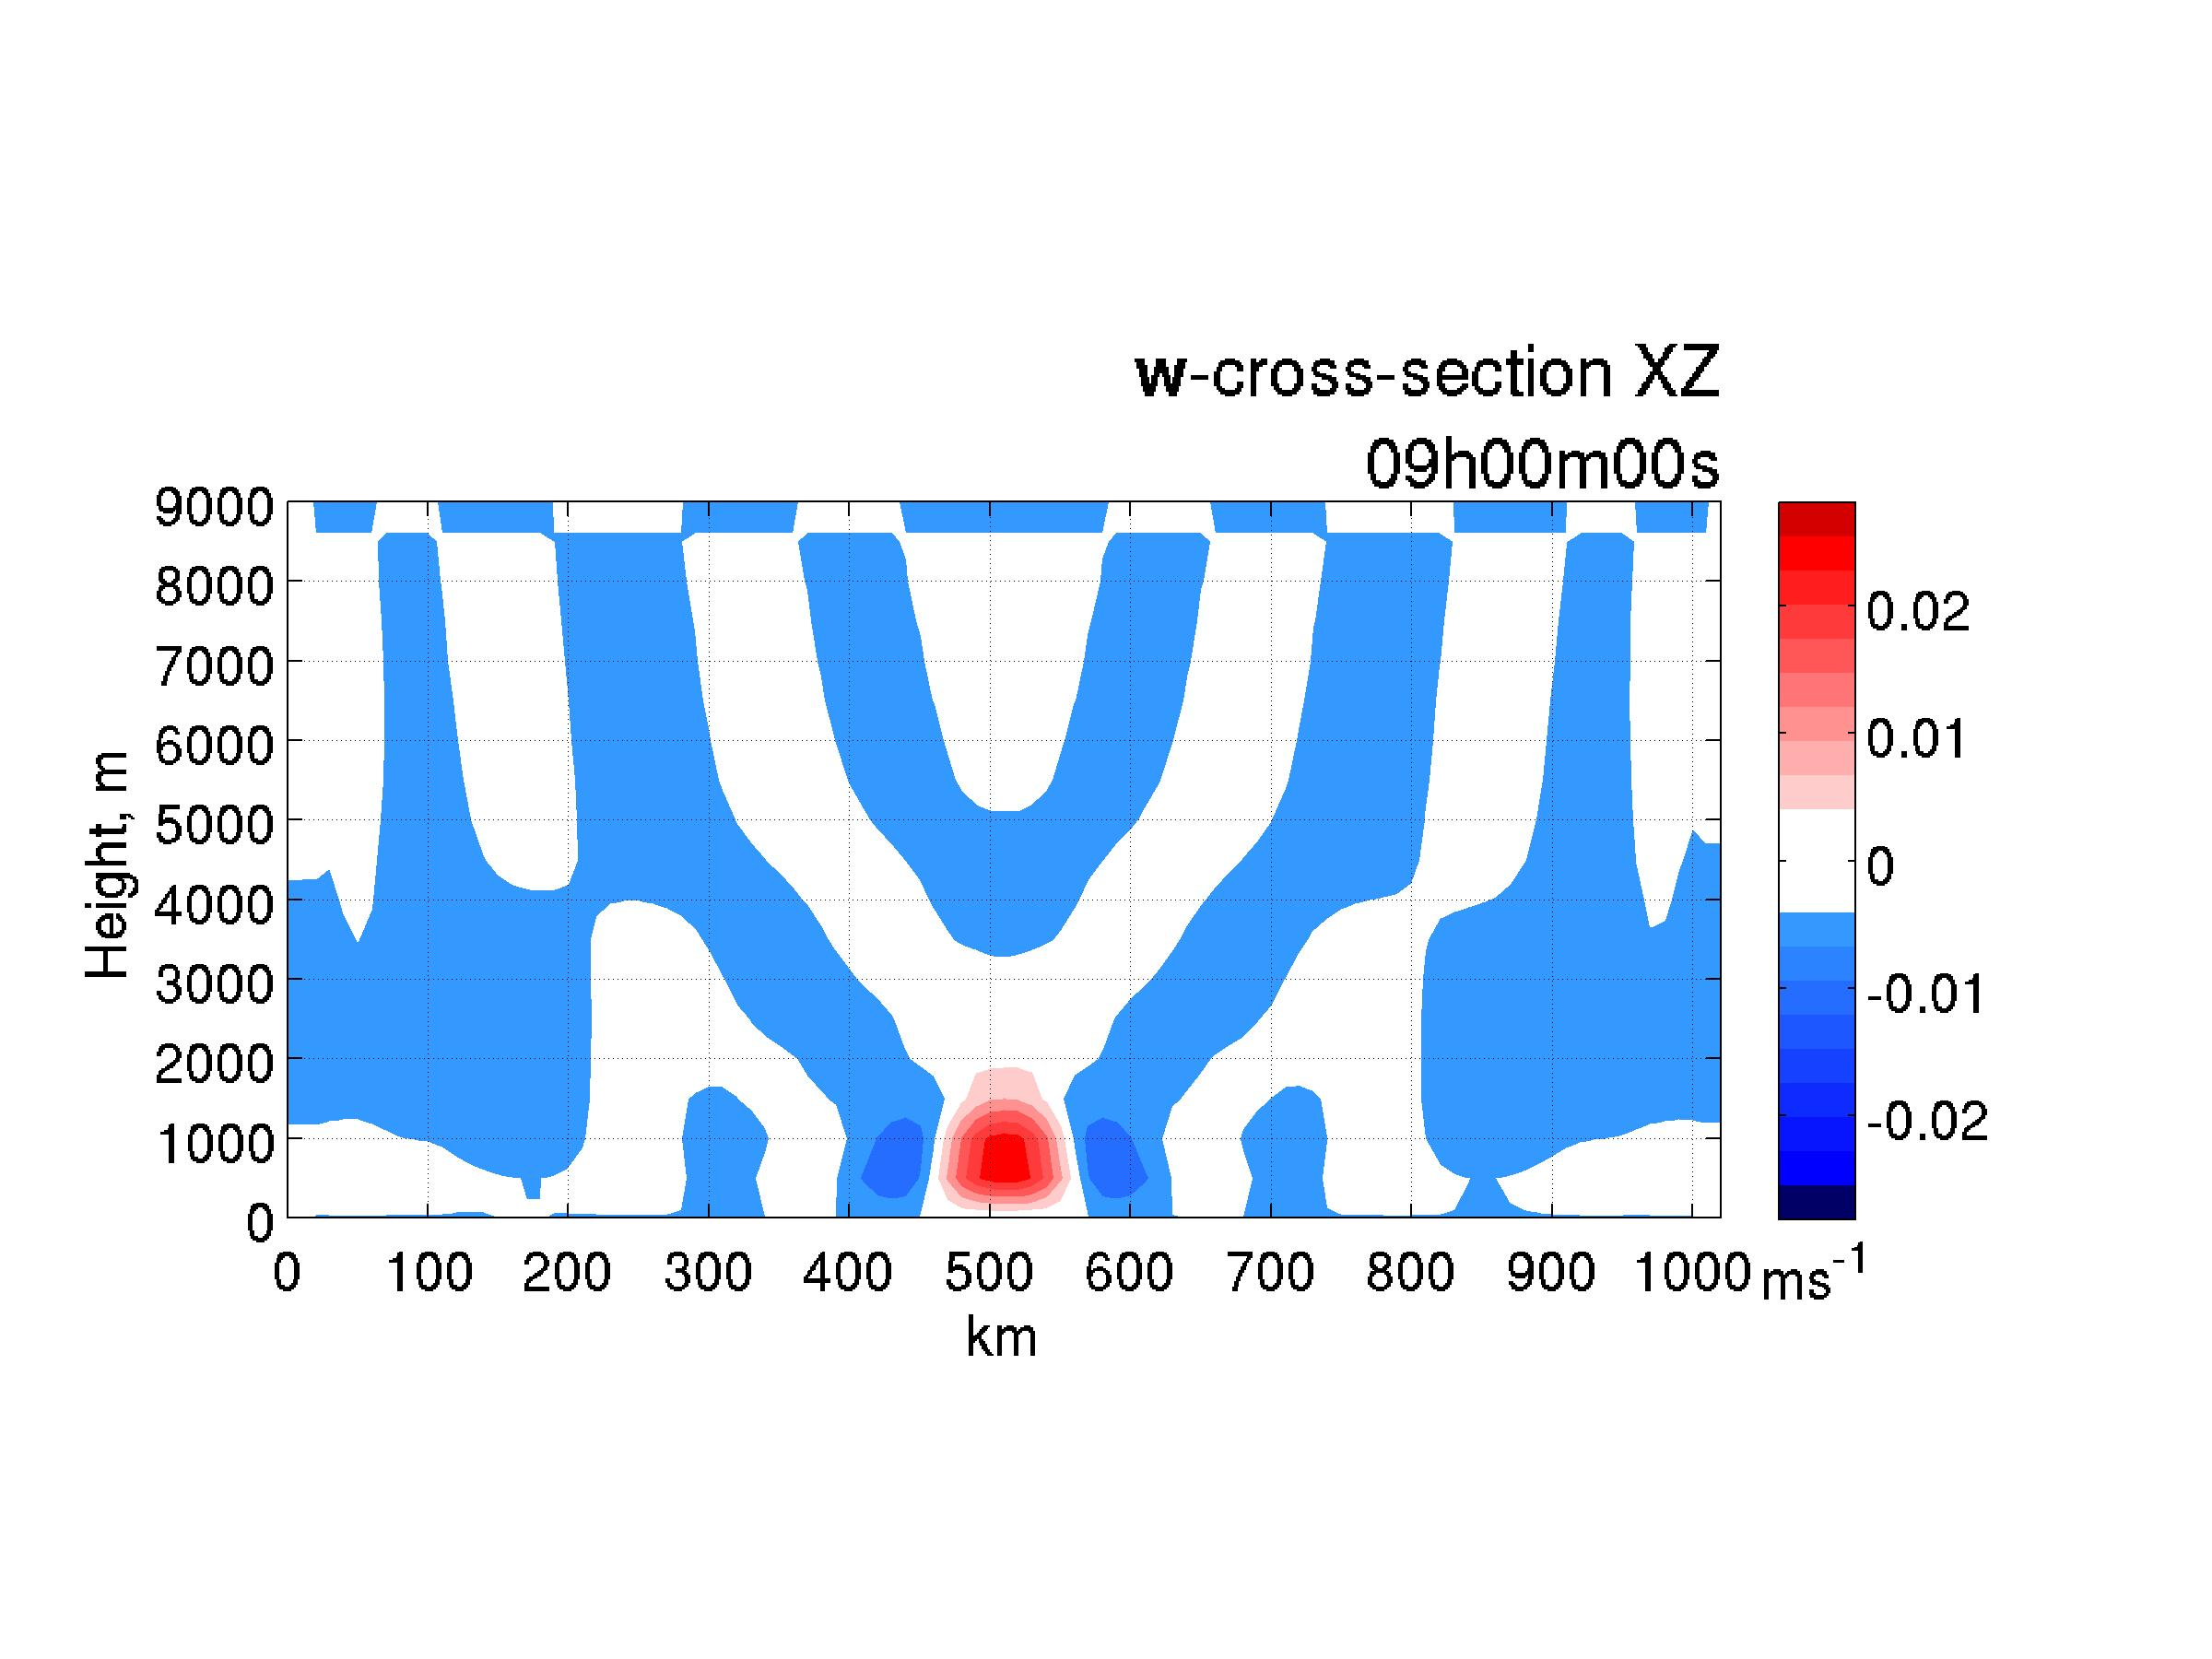
\includegraphics[width=\linewidth]{{./chapters/figures_results/ctrl_fields/W_cross_z.iy52.090000}.jpg}
\vspace{-10pt}
\caption{Меридиональный разрез вертикальной скорости $w$. Эксперимент CTRL. 9 час модельного времени.}
\label{fig:wcross}
\end{wrapfigure} 

Начальная куполообразная аномалия приводит к возникновению в нижних слоях атмосферы горизонтального градиента давления, который создает конвергенцию массы в центре области. В результате под влиянием силы Кориолиса возникают инерционно-гравитационные волны, в то время как возникновение звуковых волн невозможно ввиду разрешения сетки модели \citep{MillerWhite1984,MirandaPhD}. Путем излучения инерционно-гравитационных волн происходит приспособление атмосферы к градиентному балансу (\ref{fig:grwindbal}).

Разрез поля вертикальной скорости \ref{fig:wcross} дает представление о распространении гравитационных волн в ответ на температурное возмущение. Рисунок схож с результатами линейной теории \citep{Lin2007}, однако более правдоподобен из-за нелинейности процессов и интерференции волн в реальной атмосфере. При задании неоднородного фонового профиля стратификации области подъема и нисхождения воздуха, очевидно, будут иметь несимметричную форму.

Несмотря на четко различимые в начале моделирования волны, их влияние мало: аномалия потенциального вихря, определяющая циркуляцию в атмосфере, остается на месте, где она была изначально помещена. На рис. \ref{fig:grwindbal} частота проходящих через выбранные точки волн уменьшается, то есть волны с меньшими частотами остаются в вихре, а более высокочастотные волны распространяются наружу. Другими словами, возмущение потенциального вихря не переносится вместе с инерционно-гравитационными волнами \citep{RT2003}. Влияние волн, созданных начальным дисбалансом в атмосфере пренебрежимо мало по сравнению с 'равновесной' частью движения, которое связано через принцип обратимости с распределением потенциального вихря.

\begin{figure}[t]
	\centering
	\begin{subfigure}[t]{0.3\textwidth}
		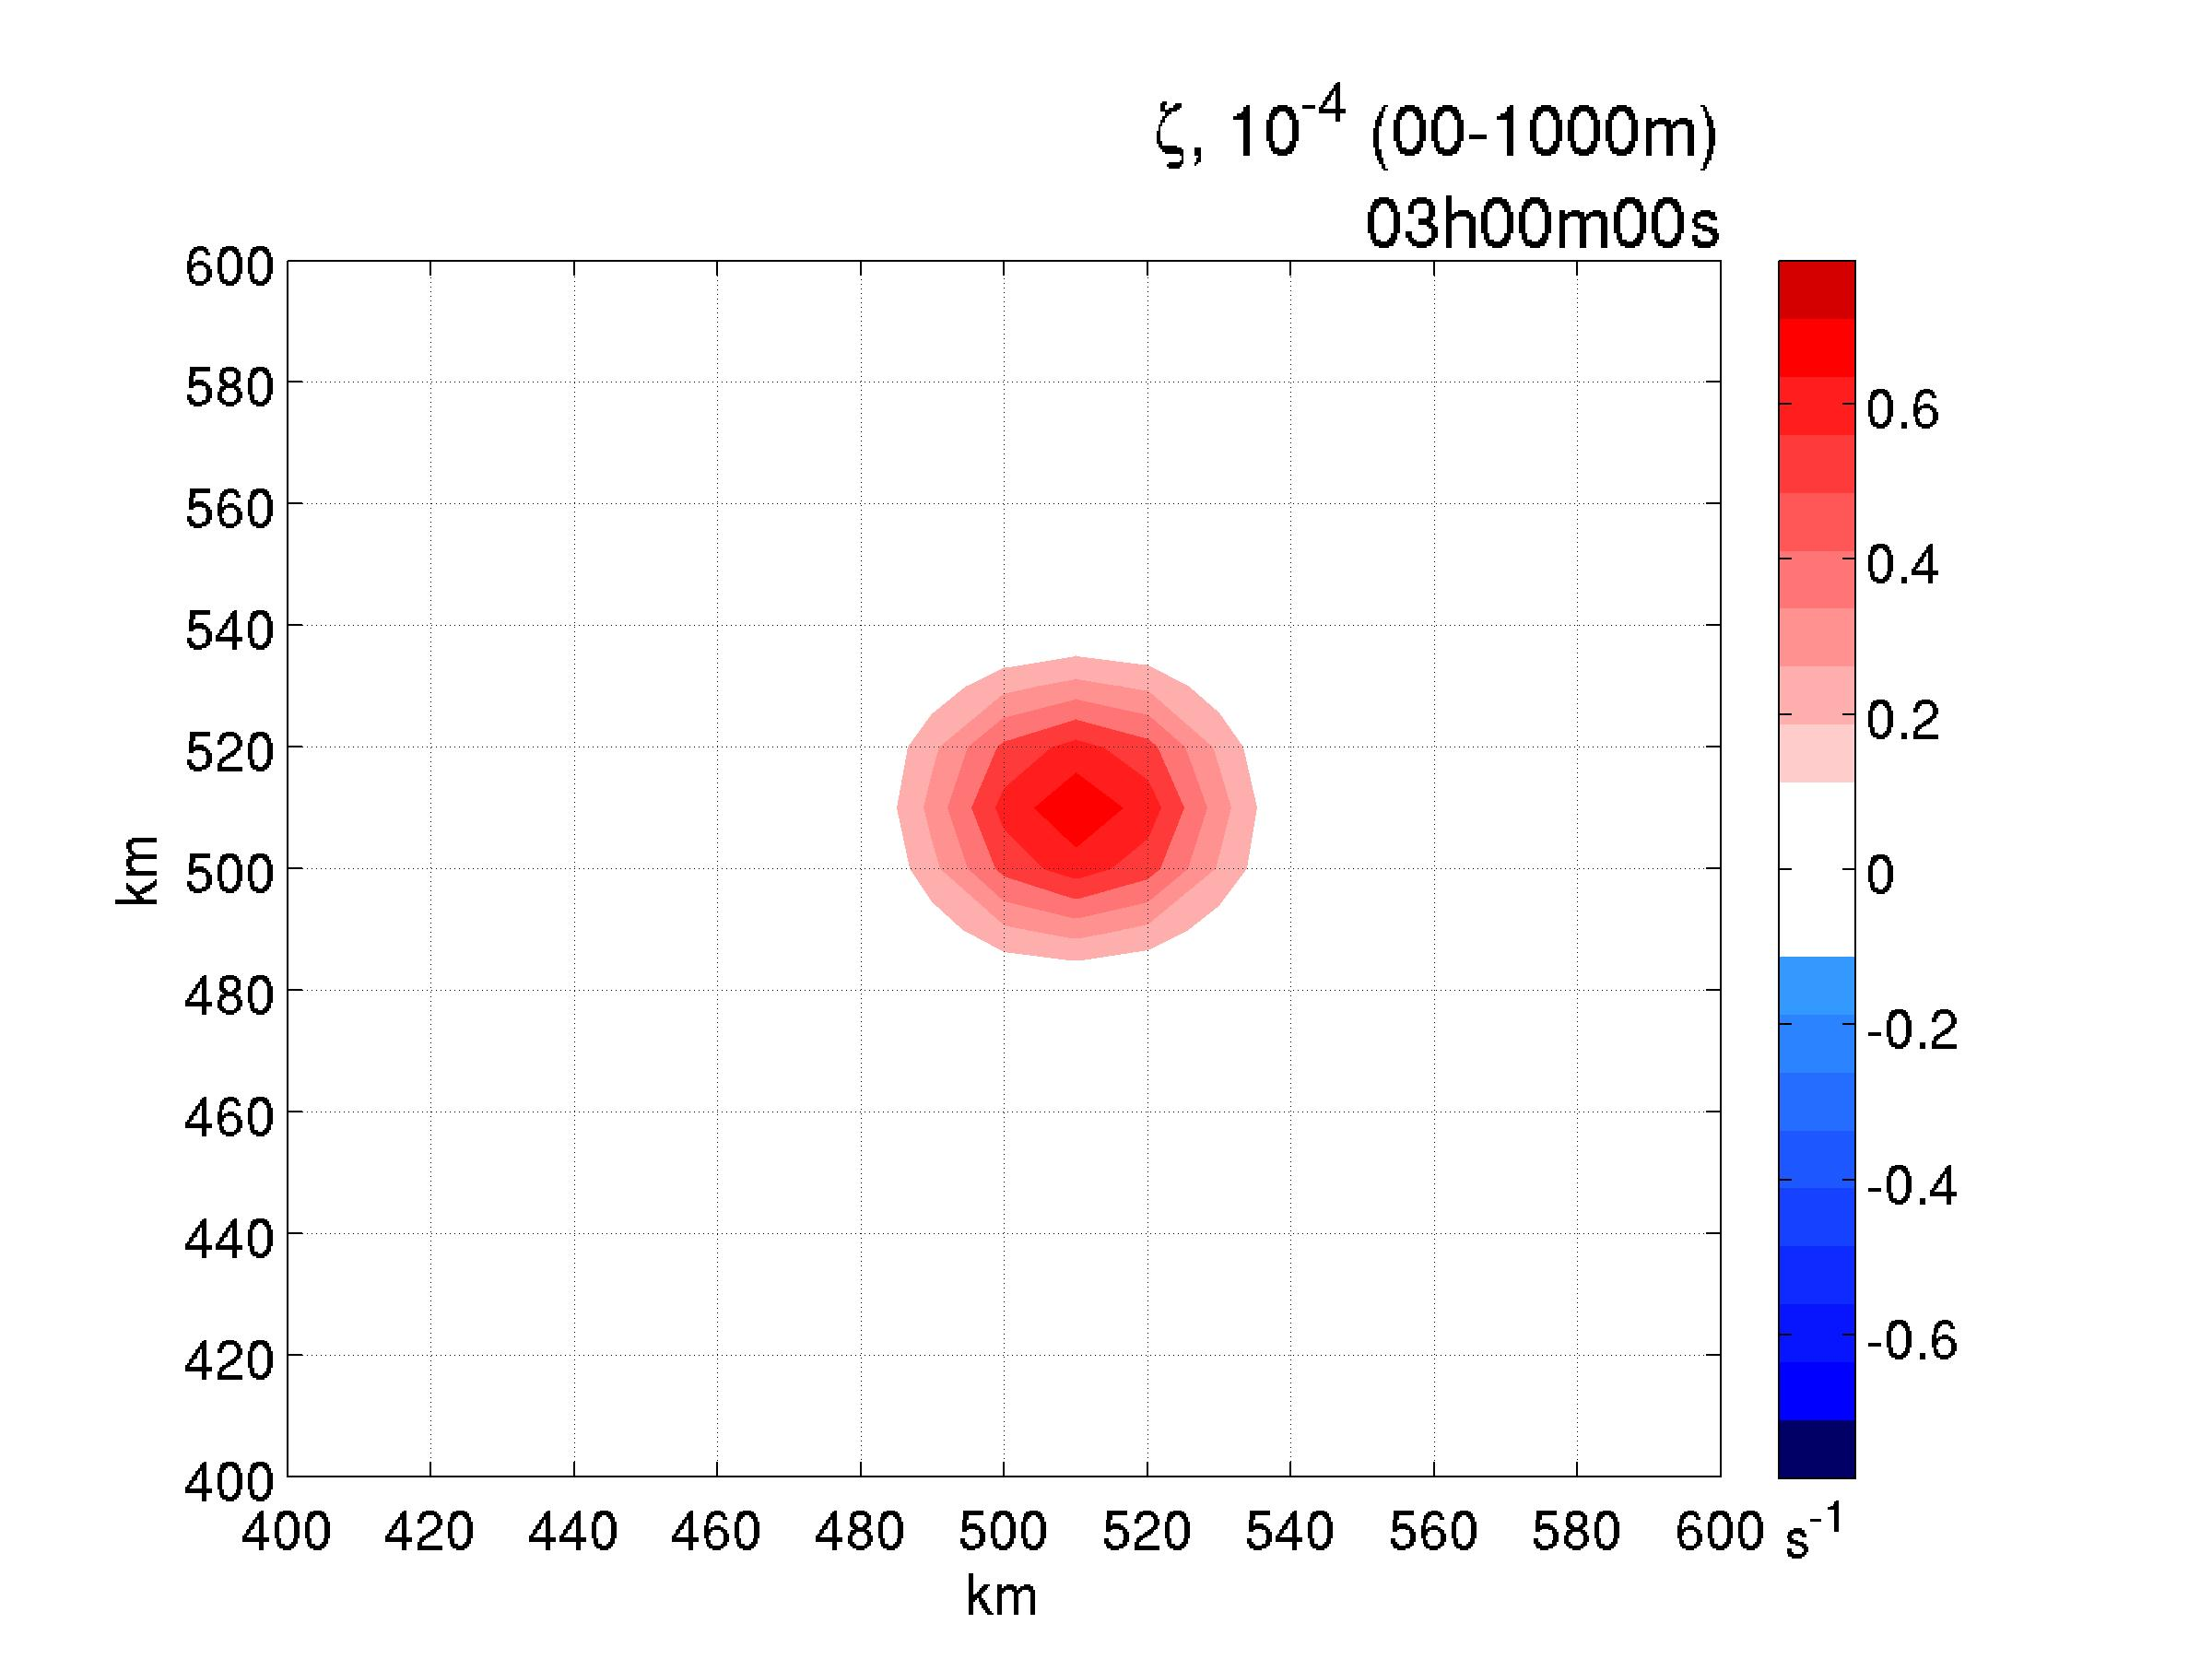
\includegraphics[width=\linewidth]{{./chapters/figures_results/ctrl_fields/rot_z_z.x41-x61.y41-y61.ilev02.030000}.jpg}
		\caption{Относительная завихренность ($\zeta$), $\pers$.}
        \label{fig:ctrl_rotz03}
	\end{subfigure}
	\hfill
	\begin{subfigure}[t]{0.3\textwidth}
		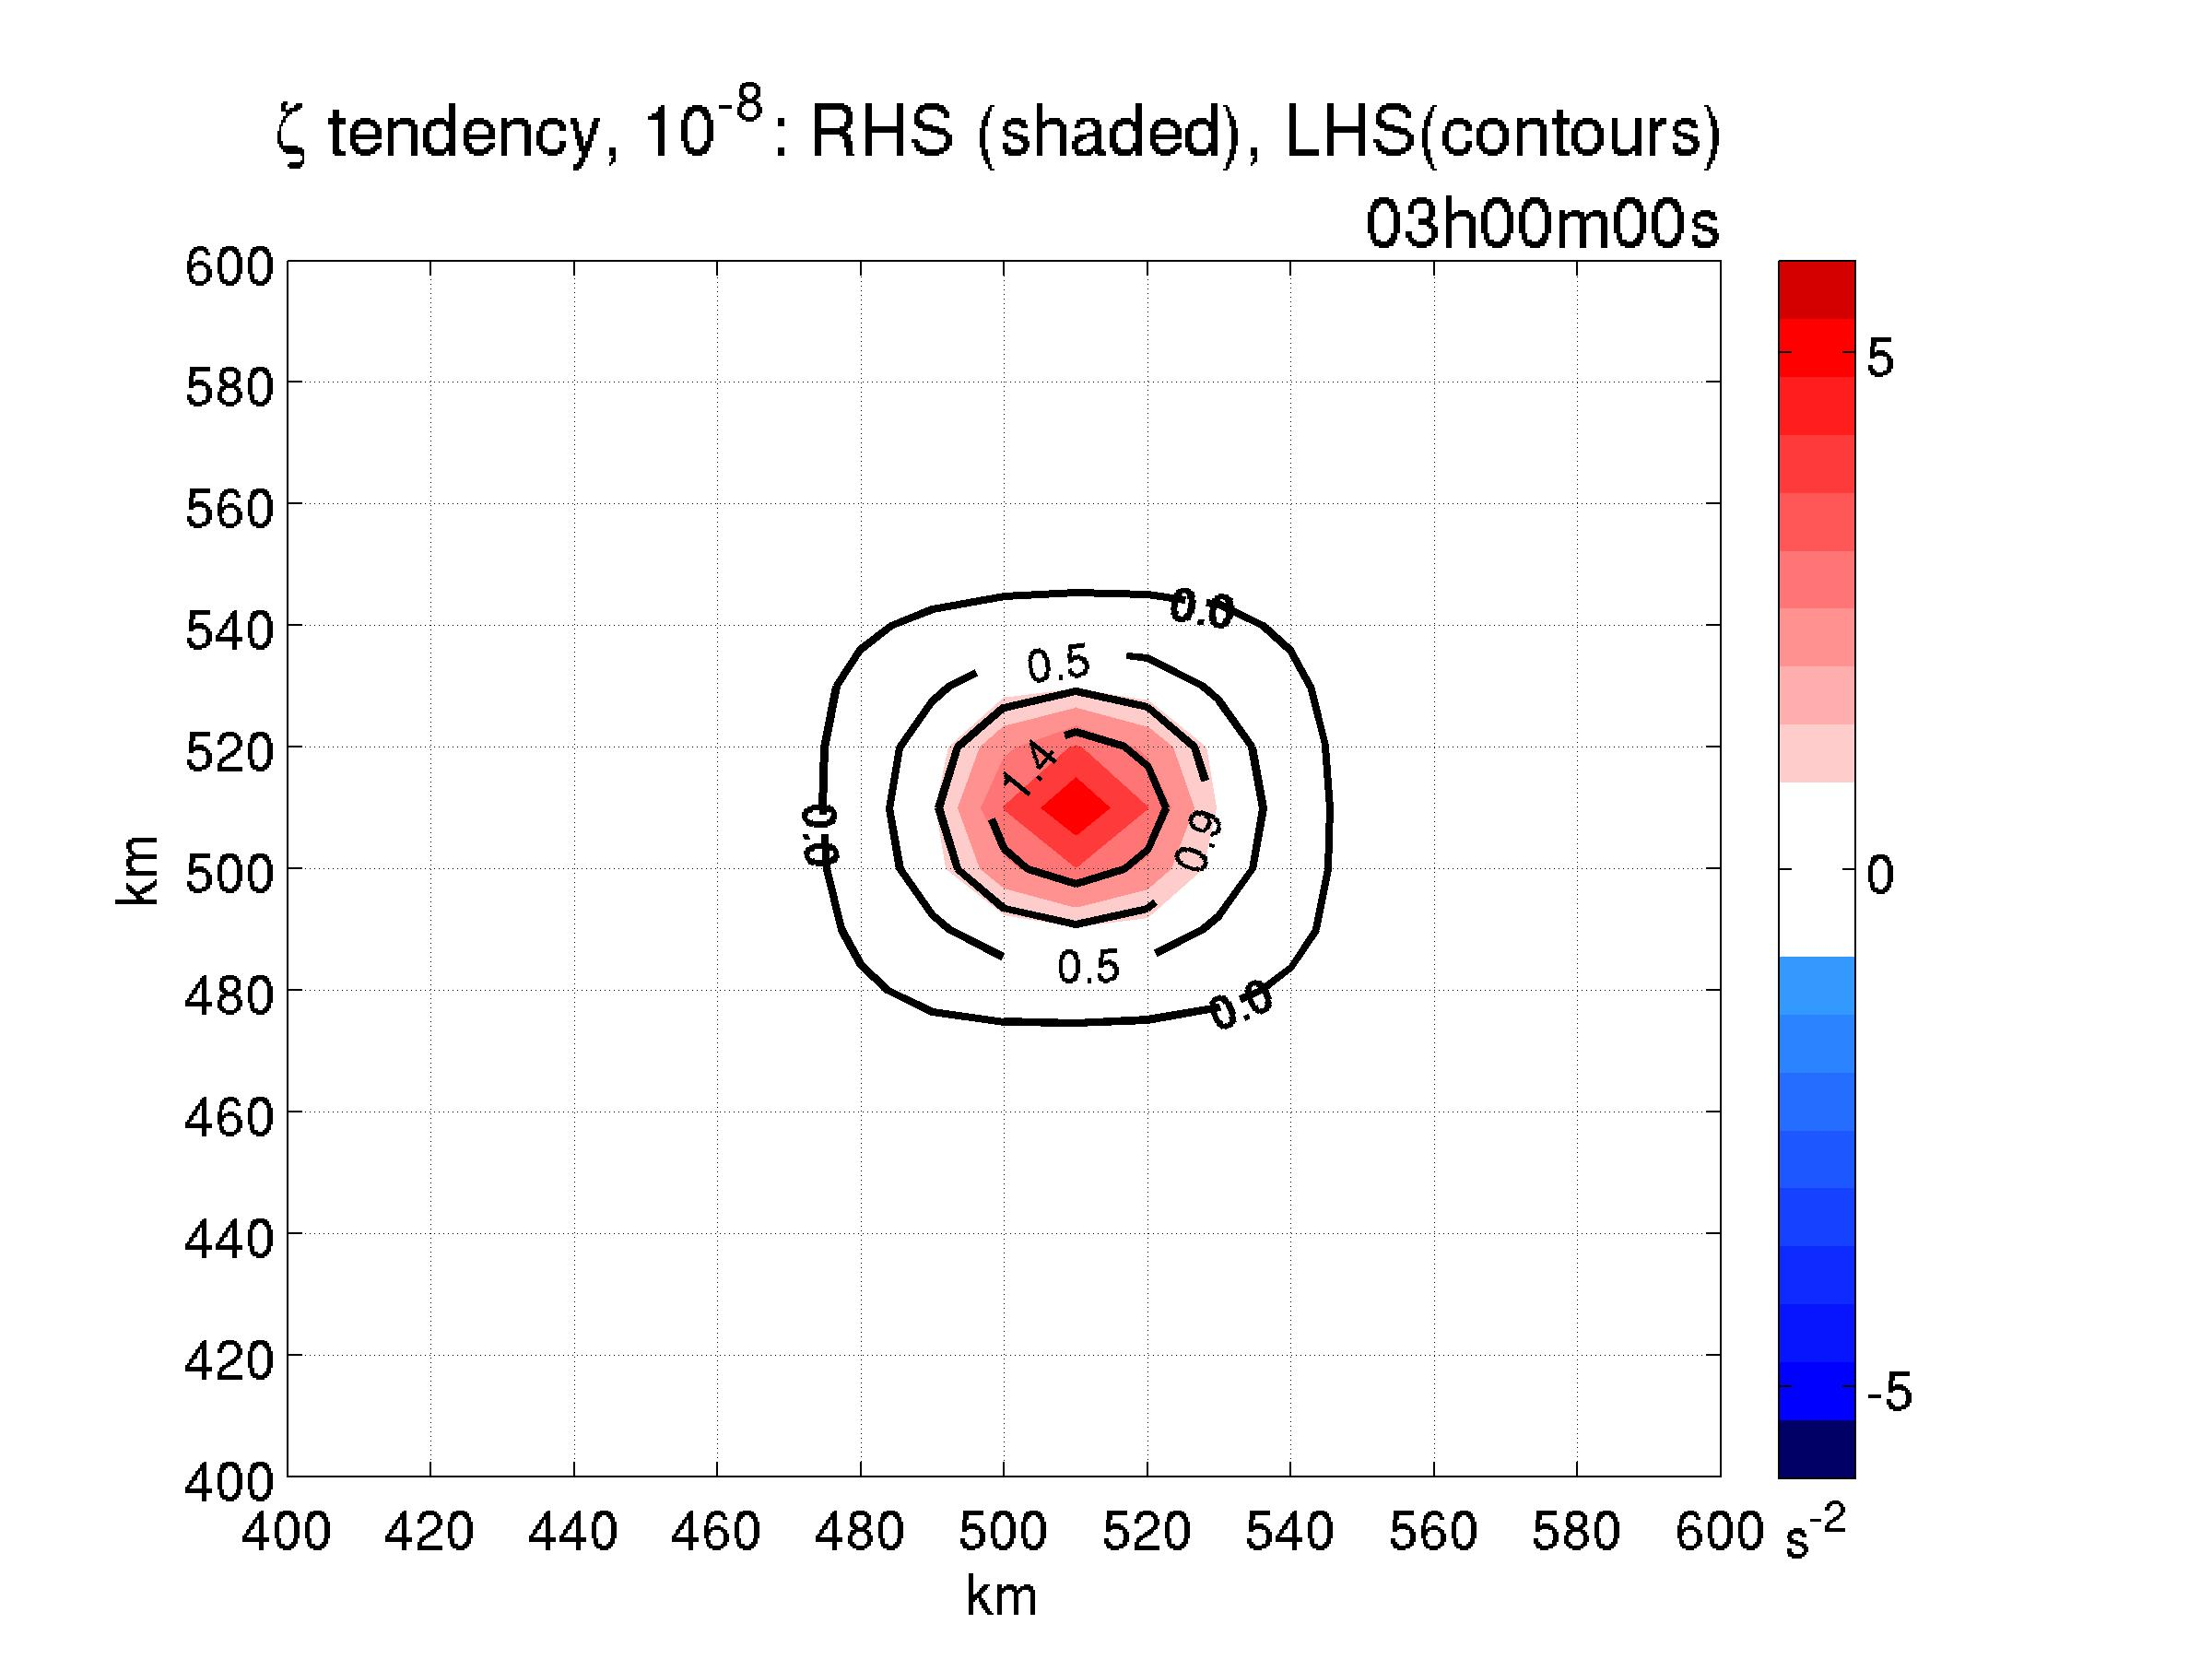
\includegraphics[width=\linewidth]{{./chapters/figures_results/ctrl_fields/vort_bud_z.x41-x61.y41-y61.ilev02.030000}.jpg}
		\caption{Тенденция относительной завихренности ($\pderiv{\zeta}{t}$), $\s^{-2}$.}
		\label{fig:ctrl_vorttend03}
	\end{subfigure}
	\hfill
    \begin{subfigure}[t]{0.3\textwidth}
		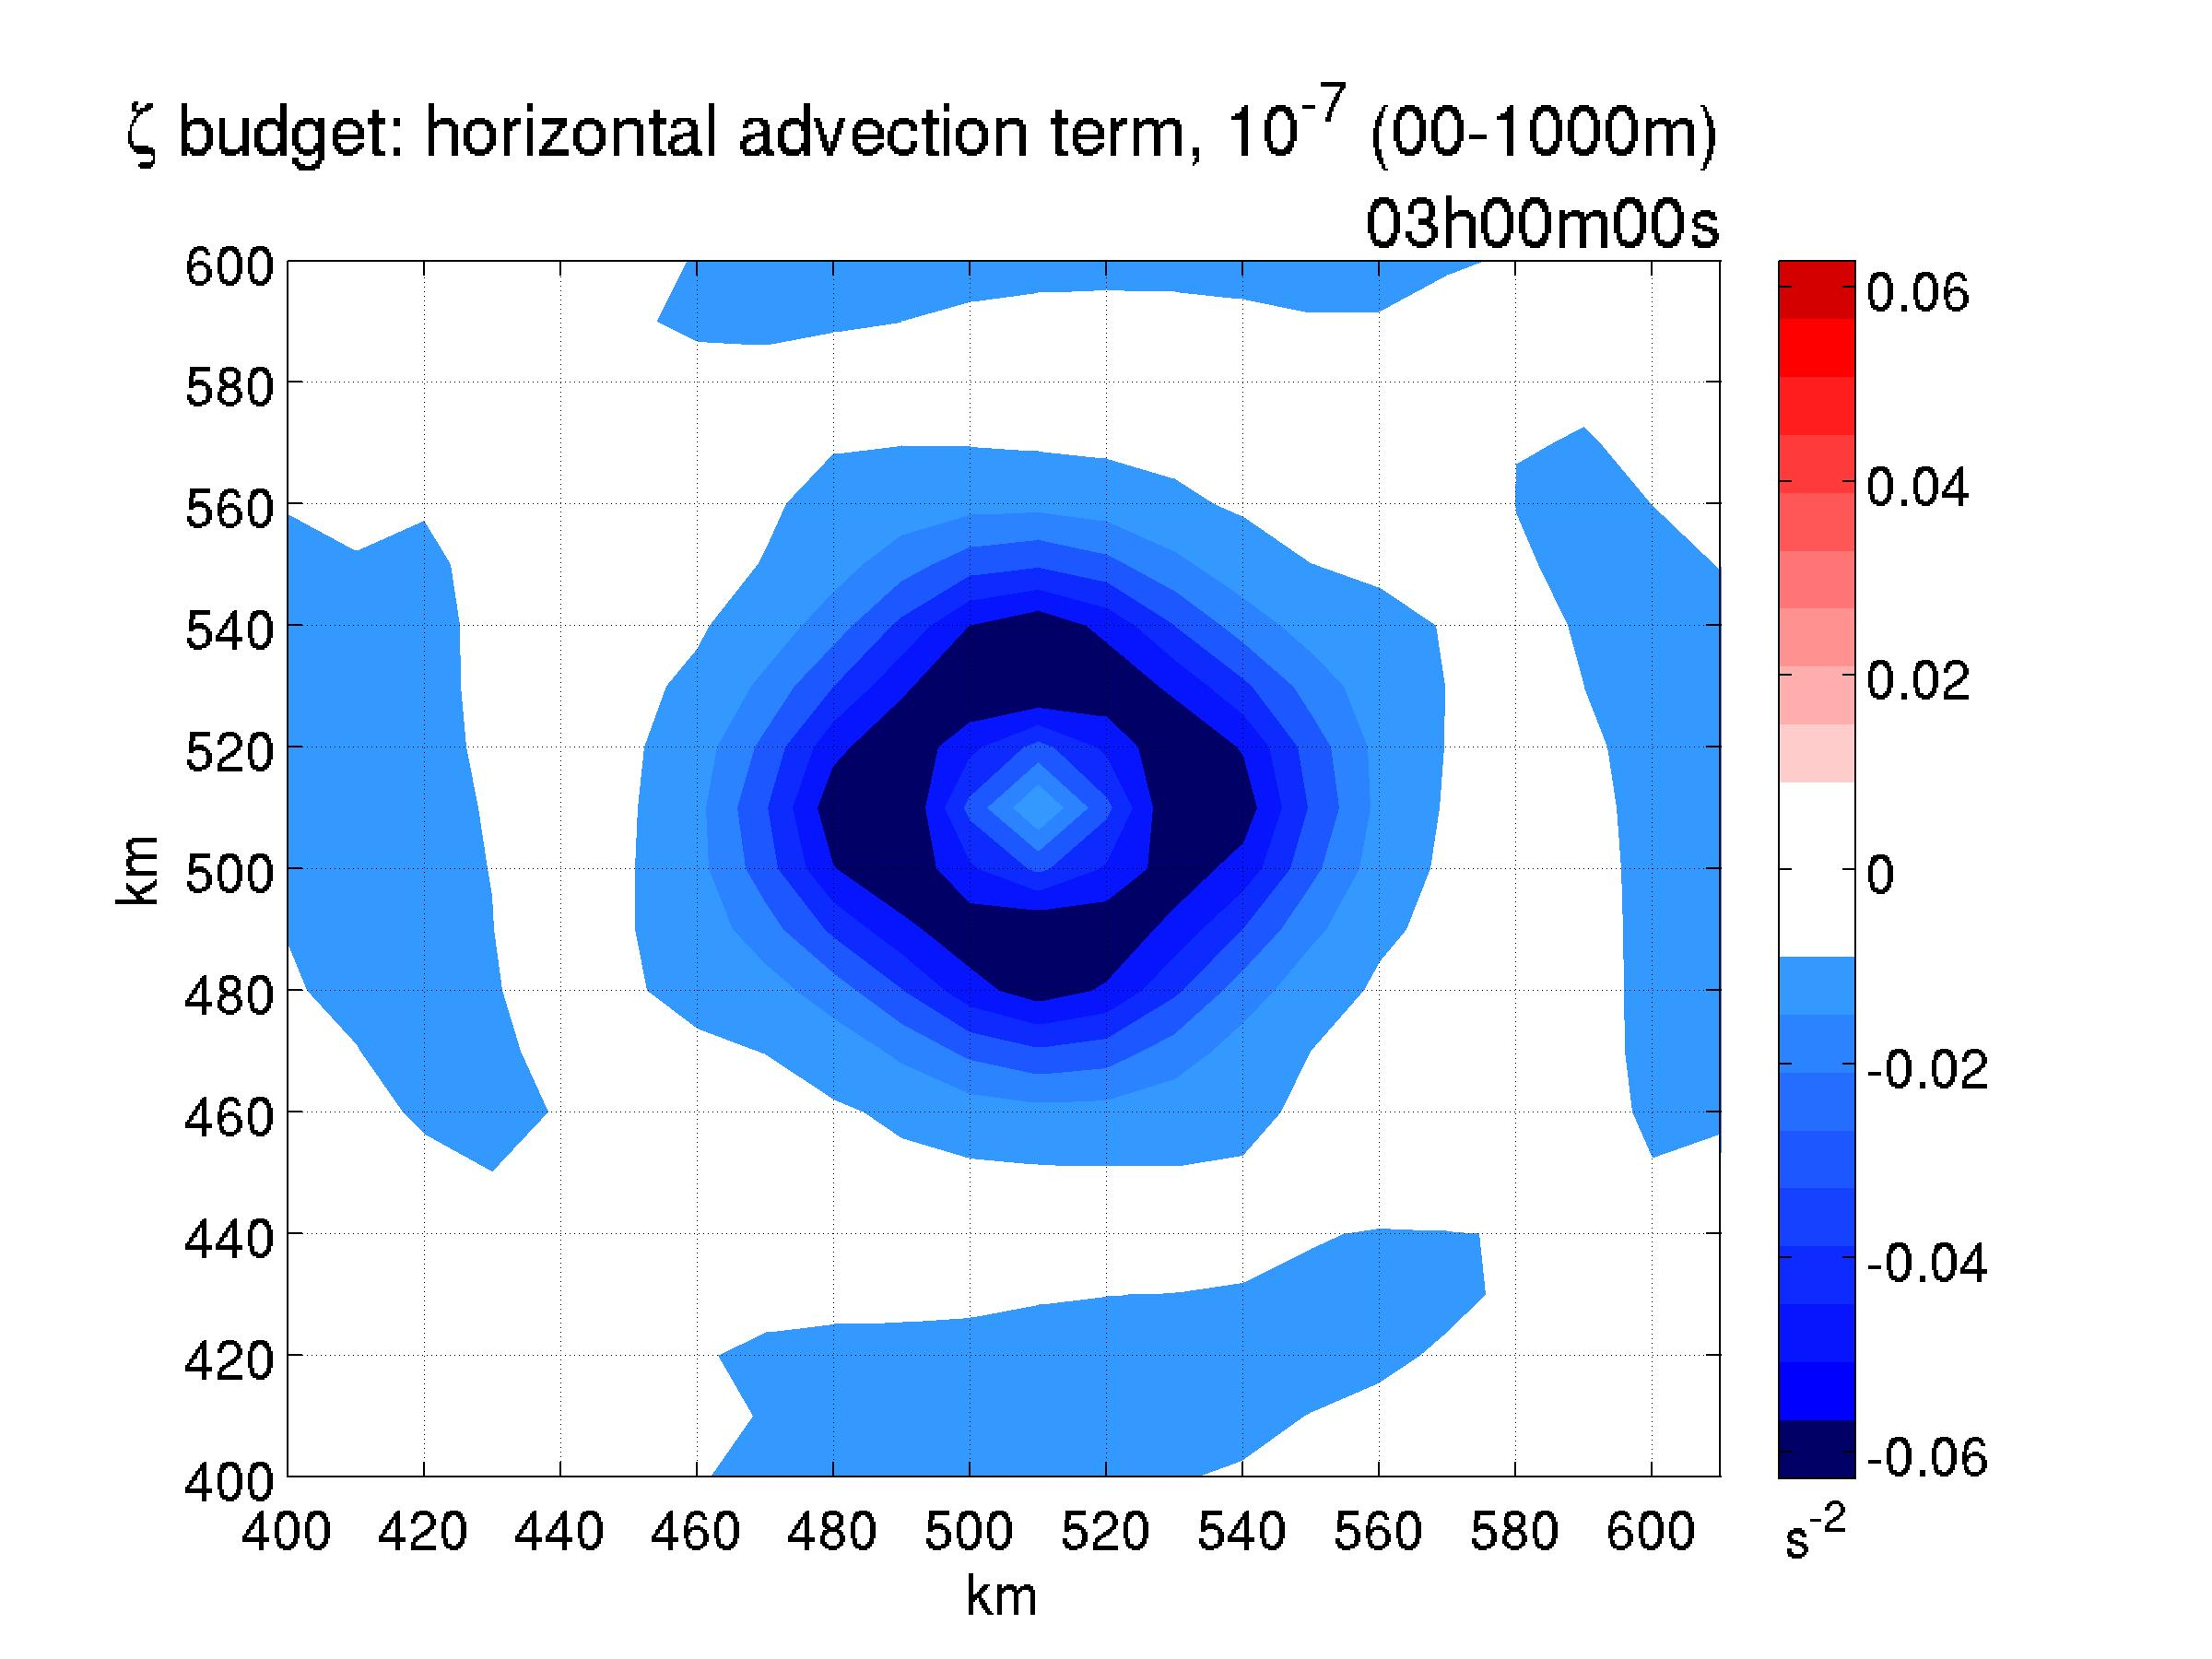
\includegraphics[width=\linewidth]{{./chapters/figures_results/ctrl_fields/vort_budget_hadv_z.x41-x62.y41-y61.ilev02.030000}.jpg}
		\caption{Слагаемое горизонтальной адвекции, $\s^{-2}$.}
		\label{fig:ctrl_hadv03}
	\end{subfigure}
	\hfill
	\begin{subfigure}[t]{0.3\textwidth}
		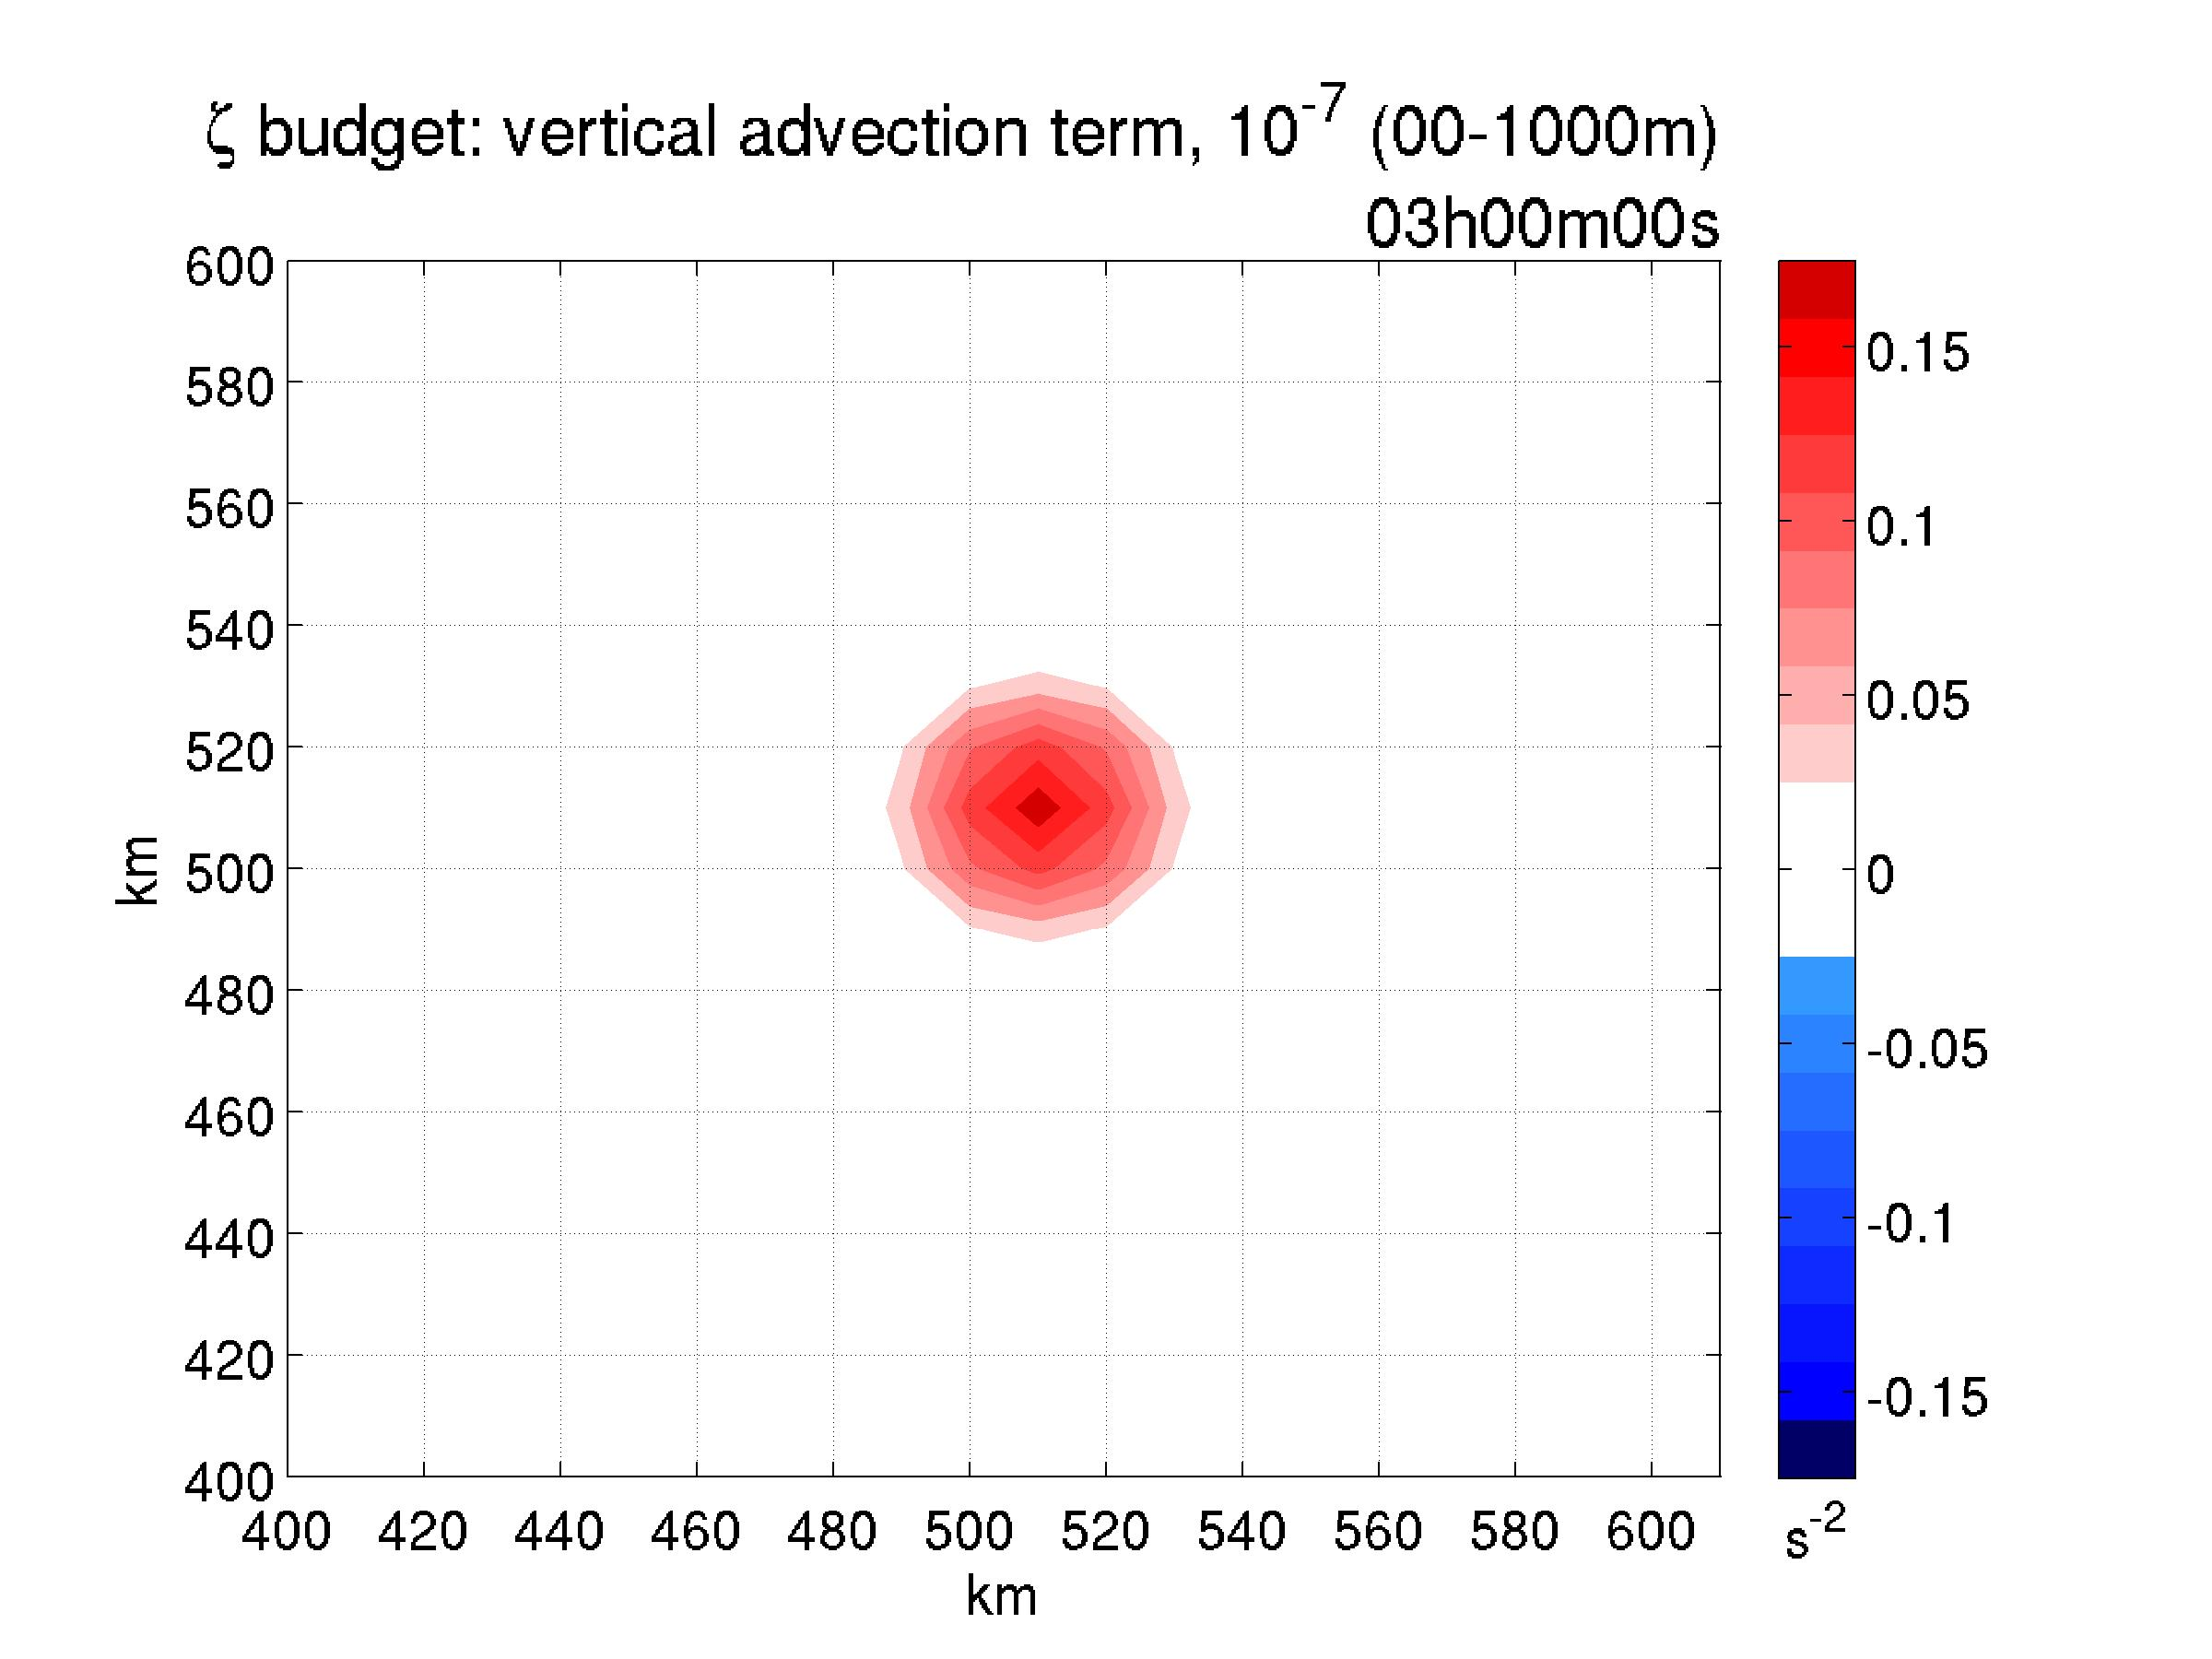
\includegraphics[width=\linewidth]{{./chapters/figures_results/ctrl_fields/vort_budget_vadv_z.x41-x62.y41-y61.ilev02.030000}.jpg}
		\caption{Слагаемое вертикальной адвекции, $\s^{-2}$.}
		\label{fig:ctrl_vadv03}
	\end{subfigure}
	\hfill
	\begin{subfigure}[t]{0.3\textwidth}
		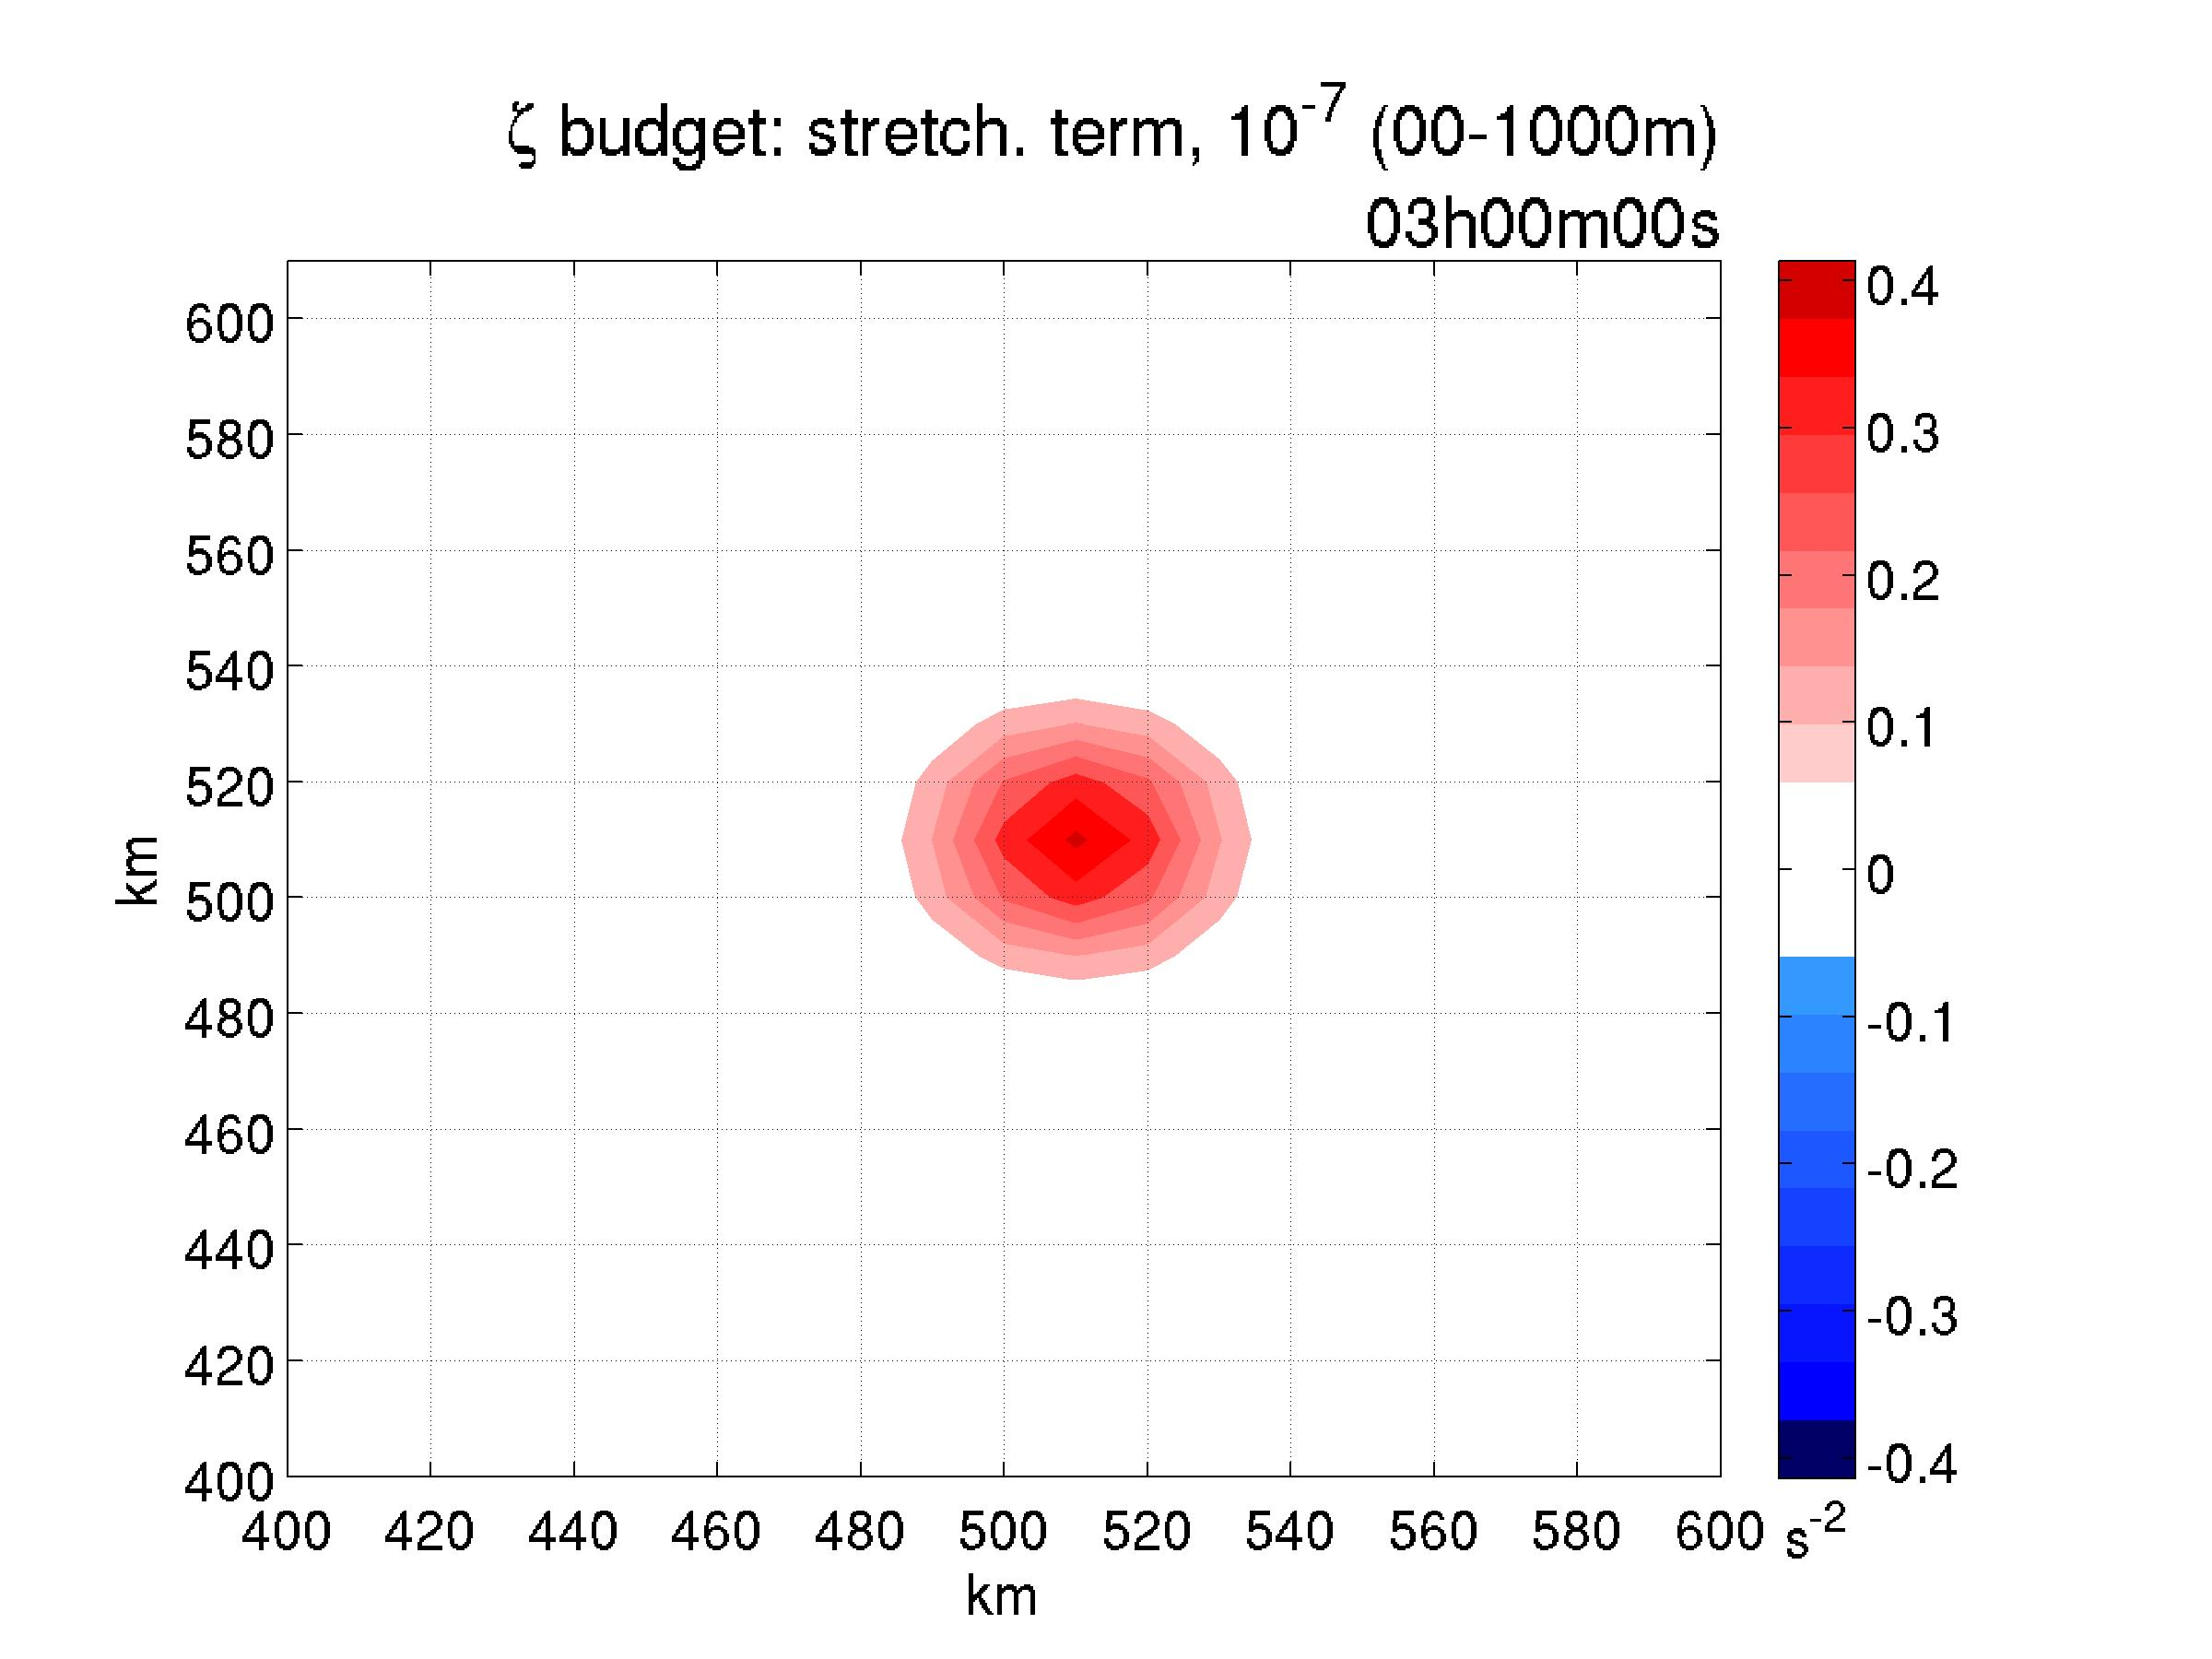
\includegraphics[width=\linewidth]{{./chapters/figures_results/ctrl_fields/vort_budget_stretch_z.x41-x62.y41-y61.ilev02.030000}.jpg}
		\caption{Слагаемое растяжения, $\s^{-2}$.}
		\label{fig:ctrl_stretch03}
	\end{subfigure}
	\hfill
	\begin{subfigure}[t]{0.3\textwidth}
		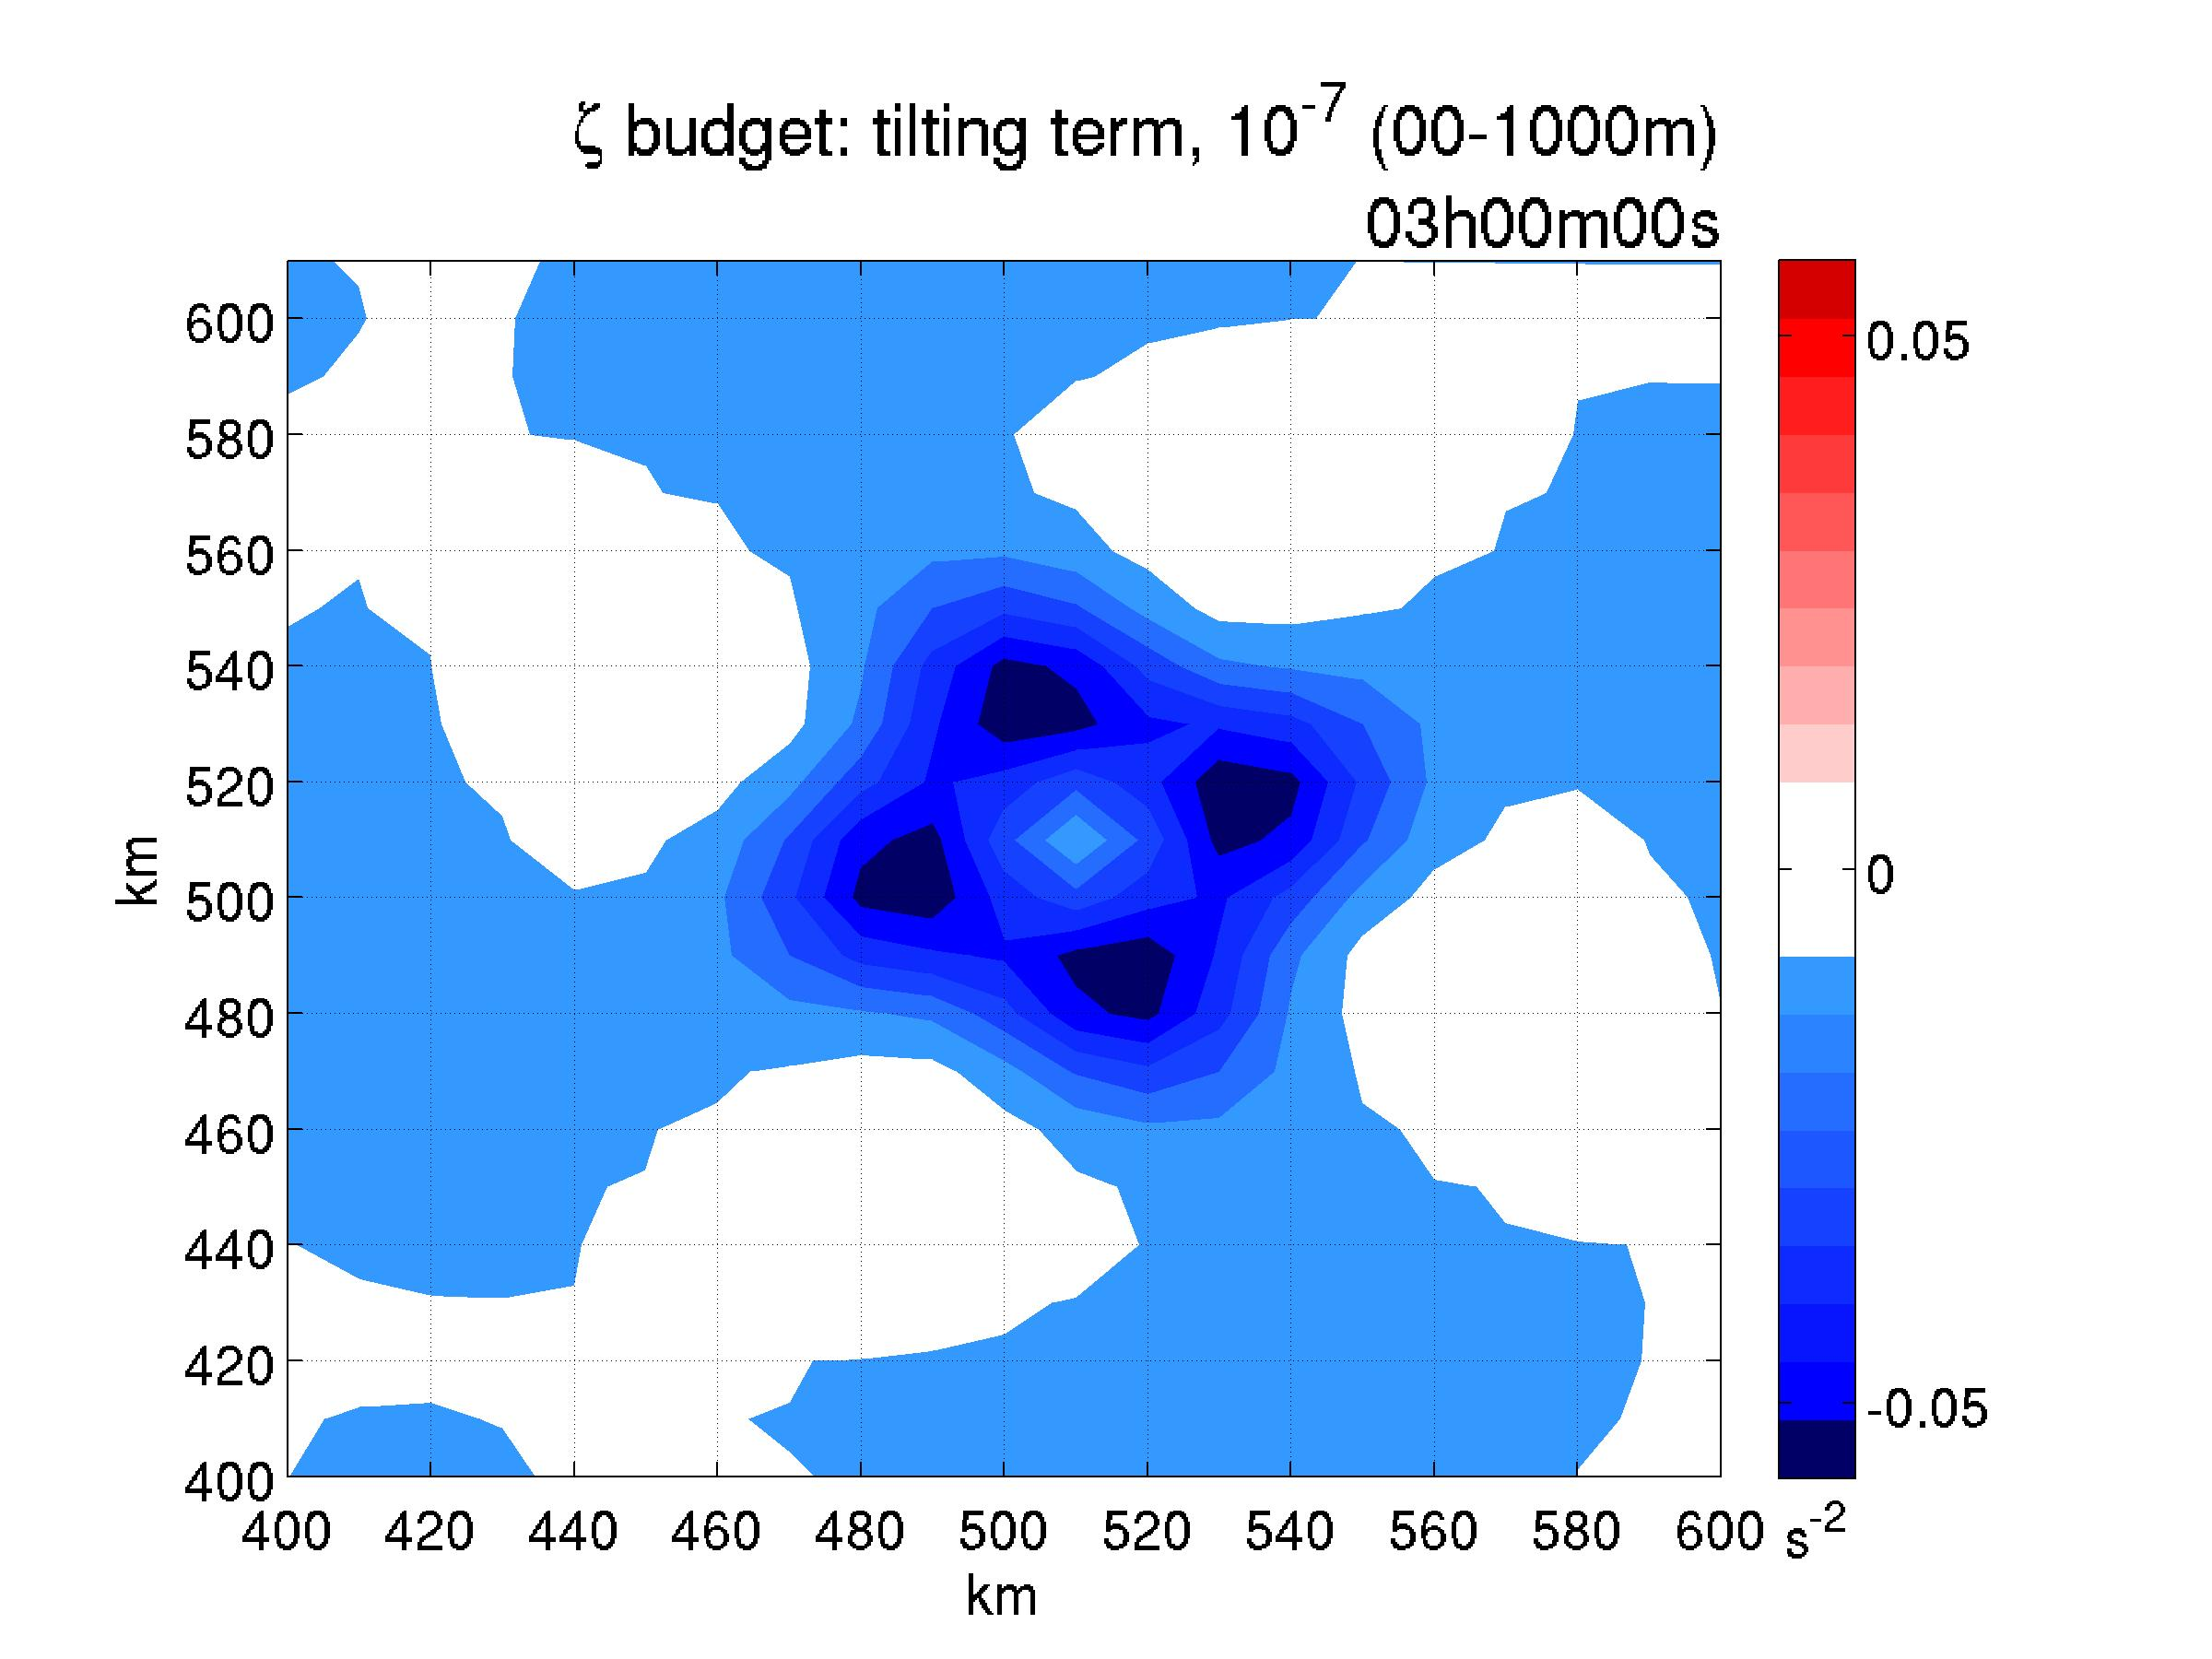
\includegraphics[width=\linewidth]{{./chapters/figures_results/ctrl_fields/vort_budget_tilt_z.x41-x62.y41-y61.ilev02.030000}.jpg}
		\caption{Слагаемое наклона, $\s^{-2}$.}
		\label{fig:ctrl_tilt03}
	\end{subfigure}
	\hfill
	\begin{subfigure}[t]{0.3\textwidth}
		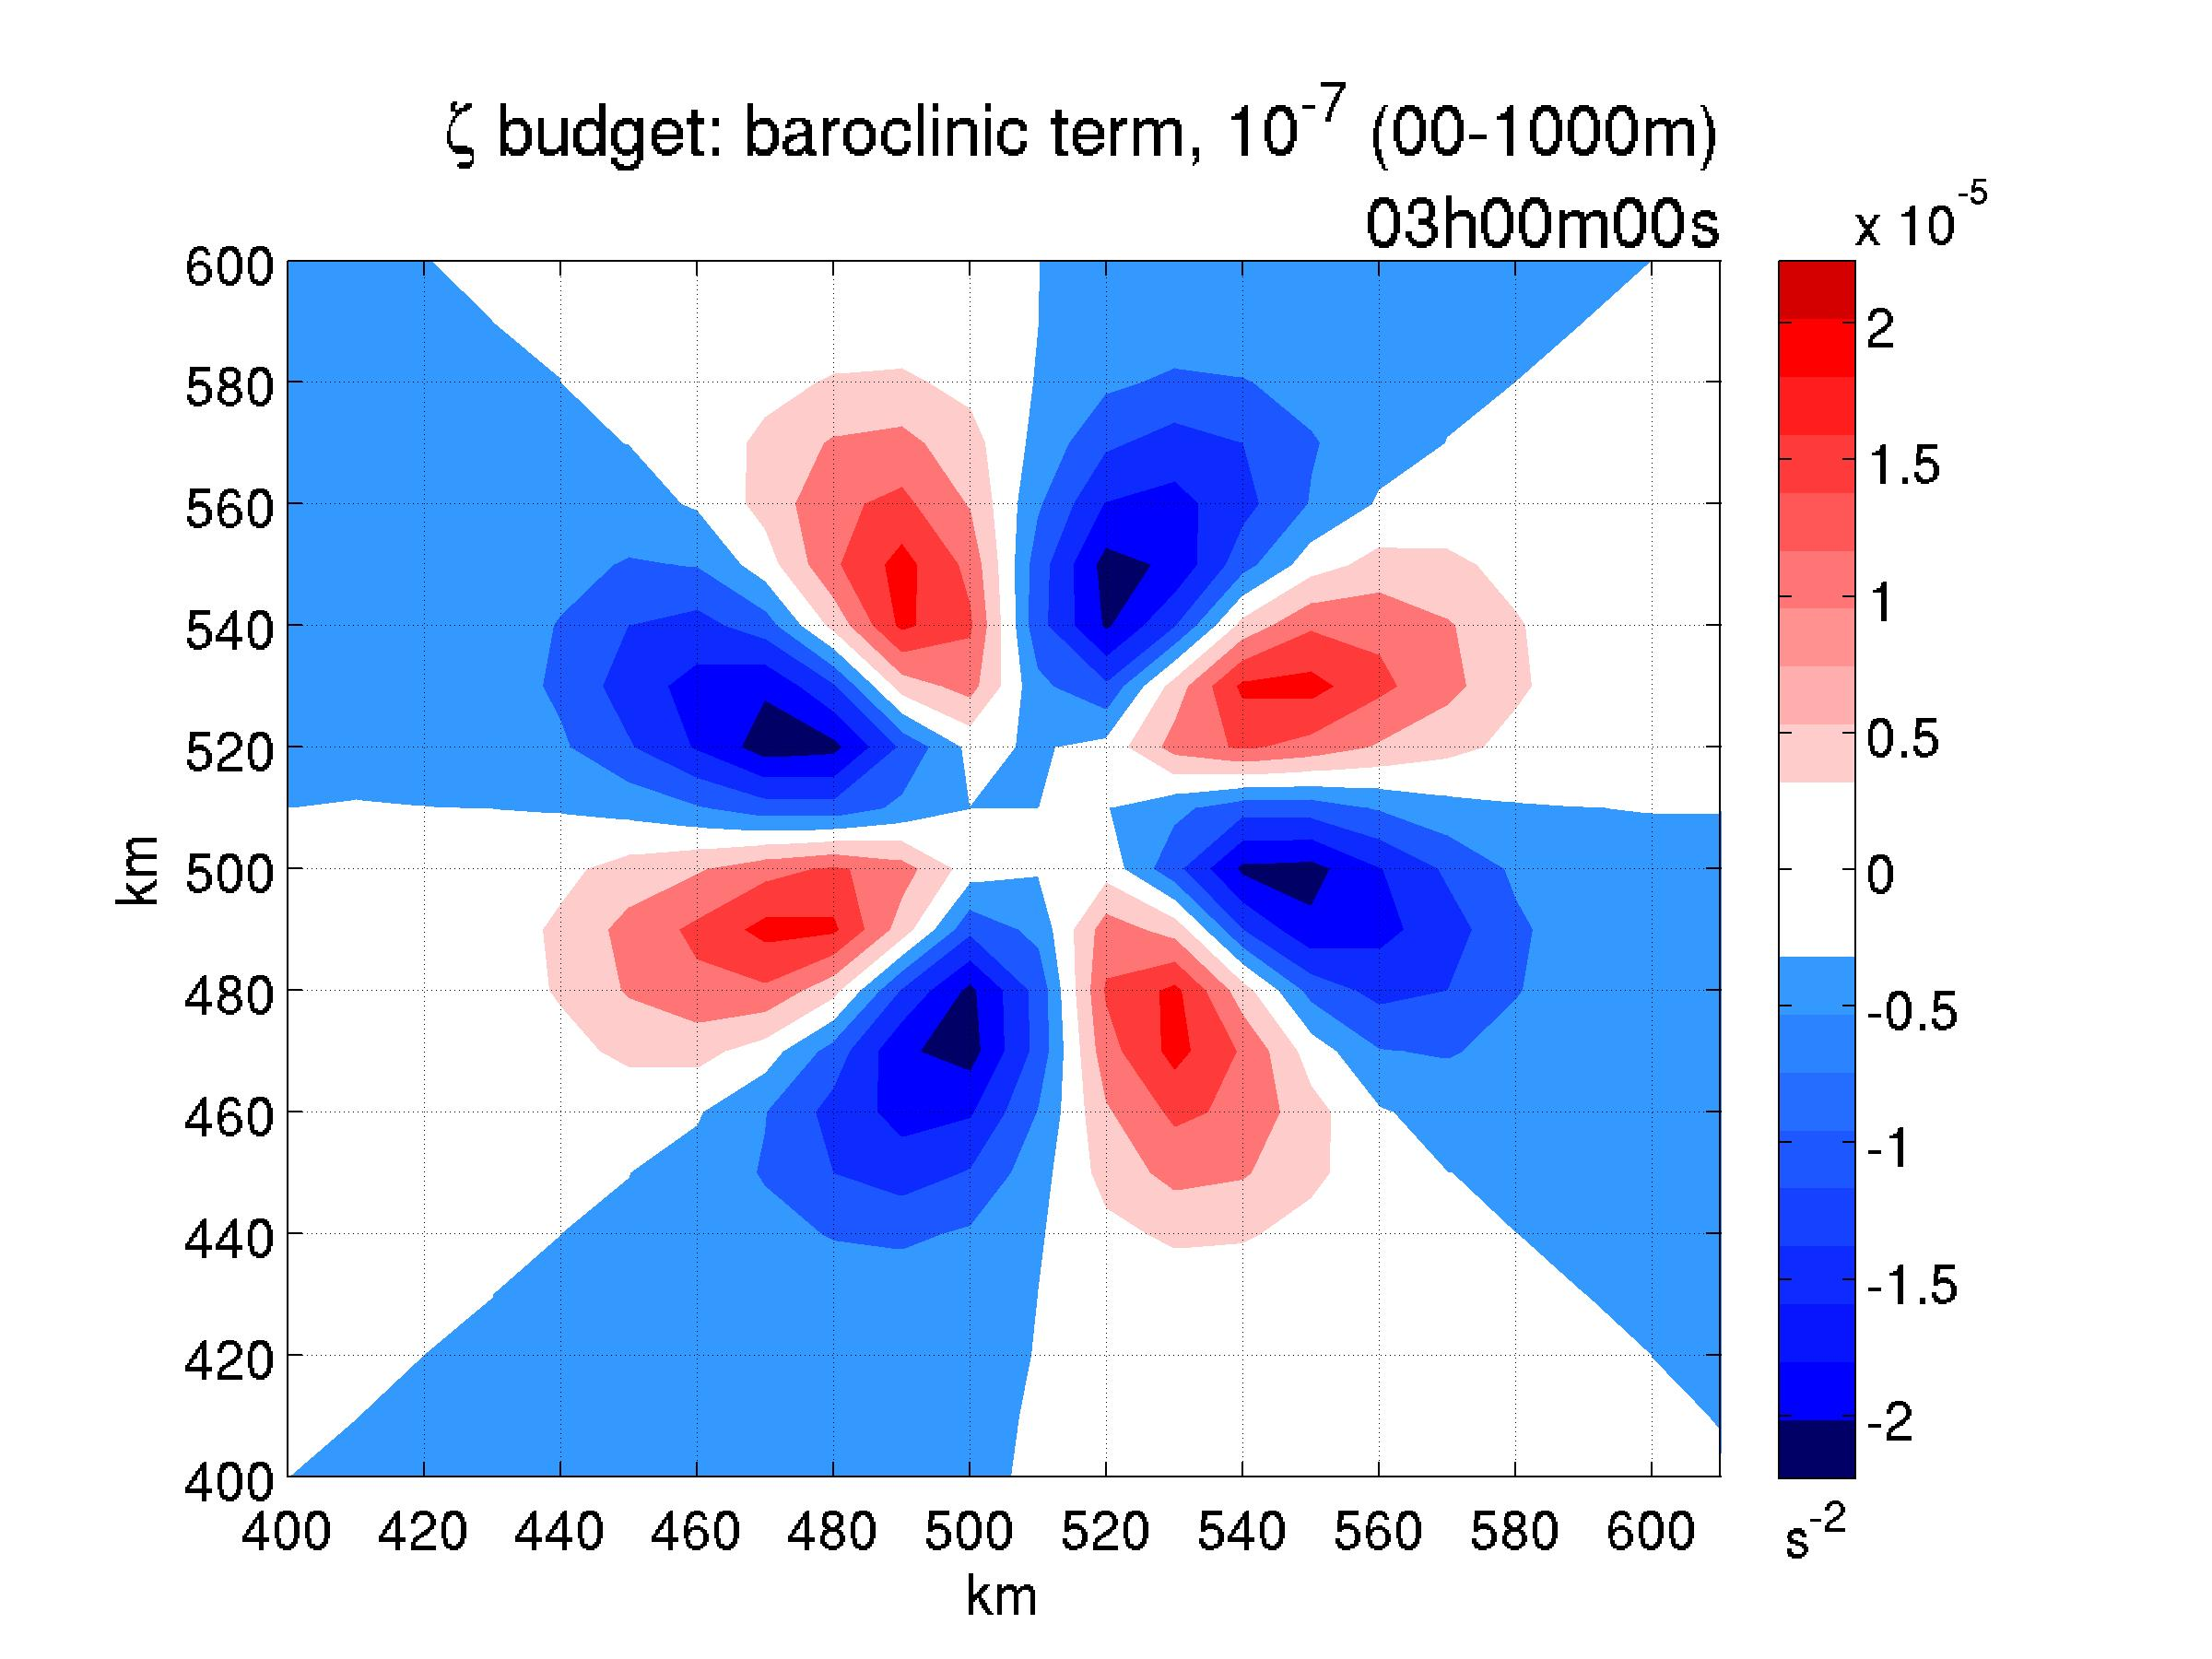
\includegraphics[width=\linewidth]{{./chapters/figures_results/ctrl_fields/vort_budget_bc_z.x41-x62.y41-y61.ilev02.030000}.jpg}
		\caption{Бароклинное слагаемое, $\s^{-2}$.}
		\label{fig:ctrl_bc03}
	\end{subfigure}
    \caption{Завихренность и бюджет завихренности в слое ниже $1000\m$. Область $200\times 200\km$, 3 час модельного времени.}
    \label{fig:ctrl_vortbud03}
\end{figure}

Равновесная часть движения формируется сразу после инициализации температурной аномалии. Подтверждением того, что наибольший вклад в развитие циркуляции имеет конвергенция массы, служит анализ уравнения завихренности \citep{Bluestein1992I} для $f$-плоскости (слагаемые, содержащие параметр $\beta=\partial f/ \partial y$ и силу трения опущены):
\begin{equation}
\label{eq:vorttend}
\pderiv{\zeta}{t}=-\vec{v}\cdot \nabla_z \zeta - w\pderiv{\zeta}{z} - (\zeta + f)\left(\pderiv{u}{x}+\pderiv{v}{y}\right) 
+ \vec{k}\cdot\left(\pderiv{\vec{v}}{z}\times\nabla w\right) + \vec{k}\cdot\left(\nabla p \times \nabla\alpha \right),
\end{equation}
где $\zeta$ --- вертикальная компонента вектора вихря скорости (завихренность), $\vec{v}=(u,v,w)$ --- вектор скорости, $\alpha=1/\rho$ --- удельный объем. Рассмотрим состояние эксперимента в 3 час модельного времени --- в момент, когда аномалия только что была инициализирована. На рис. \ref{fig:ctrl_vortbud03} представлены пространственное распределение компонент, входящих в правую часть ур. \ref{eq:vorttend}. Данные осреднены по вертикали в слое от $0$ до $1000\m$, в котором в течение всего времени наблюдаются наибольшие значения градиентов скорости.

Нетрудно заметить, что содержащее горизонтальную дивергенцию слагаемое (слагаемое растяжения) имеет наибольшие значения (рис. \ref{fig:ctrl_stretch03}), причем его экстремум совпадает с экстремумом тенденции завихренности (рис. \ref{fig:ctrl_vorttend03}) и они близки по значению. Недостающую часть тенденции вихря составляет вертикальная адвекция. Величина завихренности уже достаточно велика в данный момент (приблизительно в 2 раза меньше, чем значение параметра Кориолиса), а скорость ее роста говорит о том, что меньше, чем через час значения удвоятся. Бароклинное слагаемое (ур. \ref{eq:vorttend}, последнее слагаемое) --- произведение градиентов давления и плотности --- имеет значения на 3--4 порядка меньшие остальных членов (рис. \ref{fig:ctrl_bc03}), и это соотношение сохраняется в течение всего эксперимента. Поэтому далее бароклинное слагаемое рассматриваться не будет.

\subsection{Эволюция вихря}
Общую картину динамики вихря дают графики изменения максимума завихренности в нижней тропосфере и минимума аномалии приземного давления (\ref{}). Более детально структура вихря будет рассмотрена в следующем разделе. В контрольном эксперименте не удалось получить устойчивый вихрь: интенсивность начального возмущение с возрастающей скоростью увеличивается, пока не компоненты вектора скорости не достигают критических для численной схемы модели значений. Другими словами, в контрольном эксперименте, как и в большинстве других (см. далее), вихрь растет, не достигая устойчивой фазы и не диссипируя после этого.

\begin{wrapfigure}{L}{0.5\textwidth}
\begin{center}
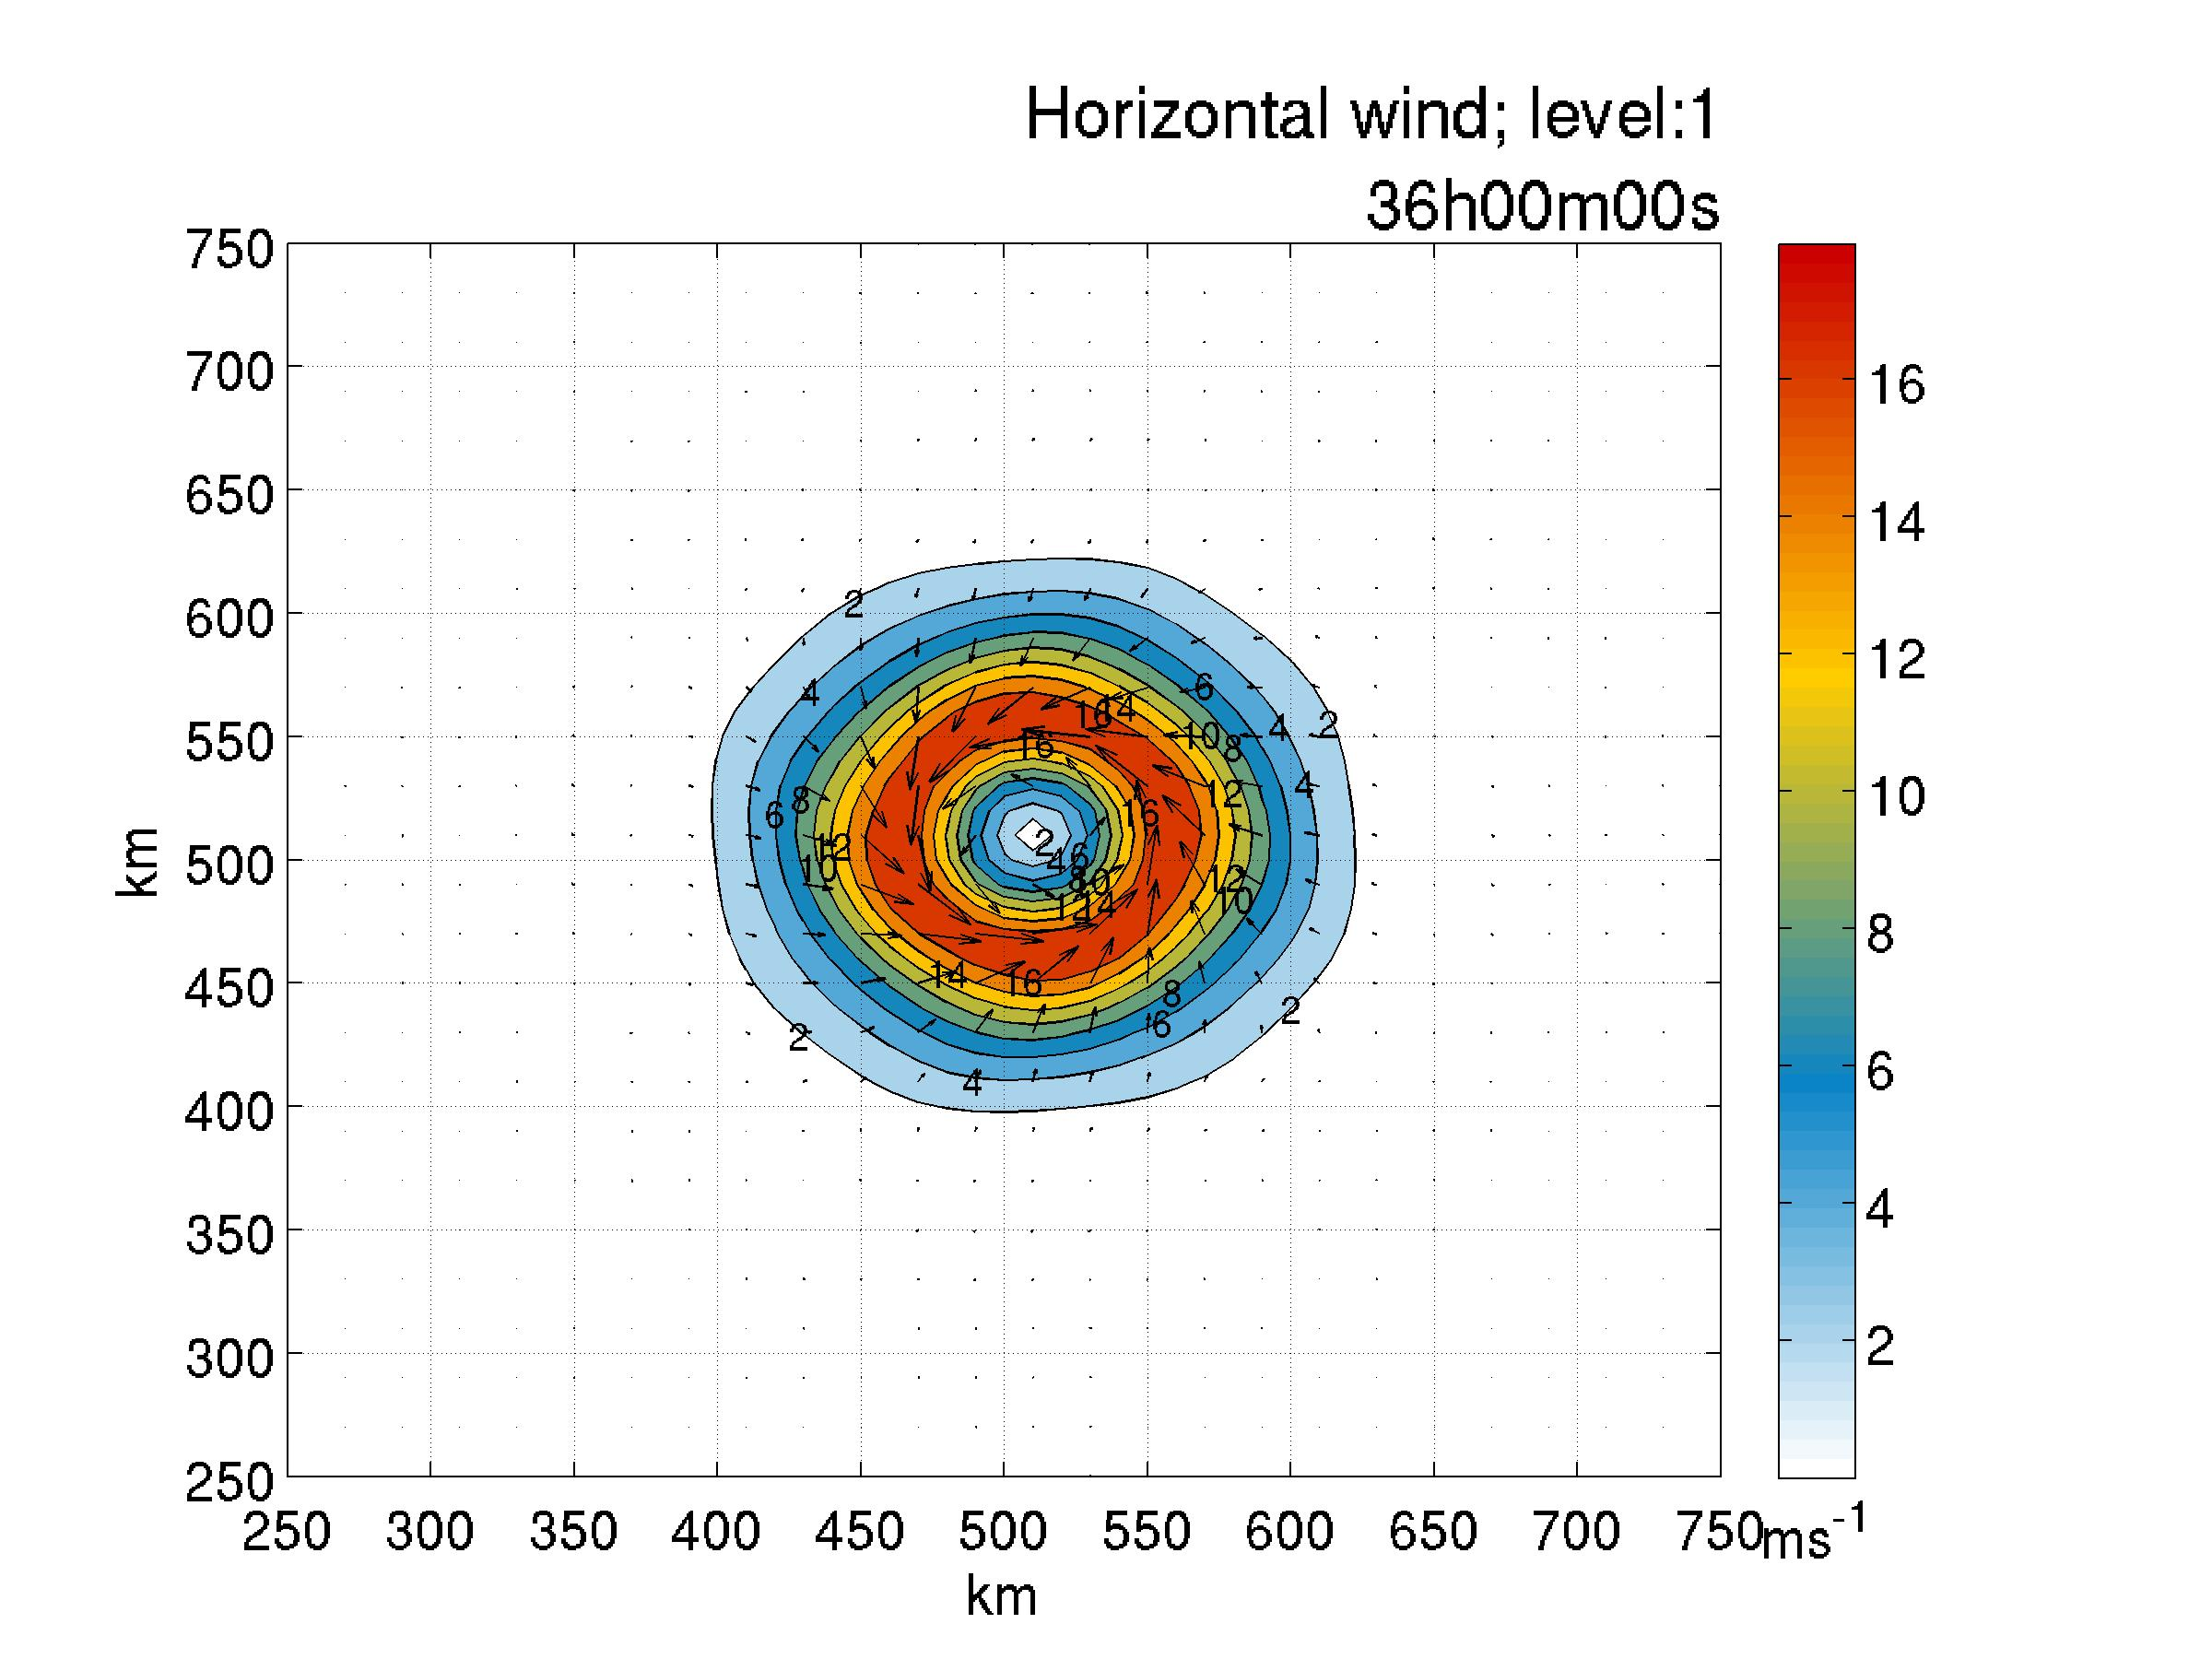
\includegraphics[width=\linewidth]{{./chapters/figures_results/ctrl_fields/VectorWind_z.x26-x76.y26-y76.ilev01.360000}.jpg}
\end{center}
\caption{Поле горизонтальной скорости ветра  (фокус $500\times 500\km$). Эксперимент CTRL. 36 час модельного времени.}
\label{fig:ctrl_hwind}
\end{wrapfigure} 

Уже в начале эксперимента относительная завихренность начинает превышать планетарную завихренность, которая для данной области равняется $\approx 1.37\pers$. Поэтому можно говорить о том, что динамика мезоциклона полностью описывается относительной завихренностью и почти не зависит от планетарной компоненты в течение своего жизненного цикла. Максимальное значение завихренности достигается на 43 ч. модельного времени и составляет $7.6\times 10^{-3}\pers$. В конце эксперимента достигается и наибольшее по модулю падение приземного давления ($-43.6\hpa$). Здесь и далее под этим понимается разность между минимальным приземным давлением и средним по области приземным давлением:
\begin{equation} \label{eq:slpanom}
SLP_{anom}=SLP_{min}-\overline{SLP}.
\end{equation}

\begin{wrapfigure}{L}{0.5\textwidth}
\begin{center}
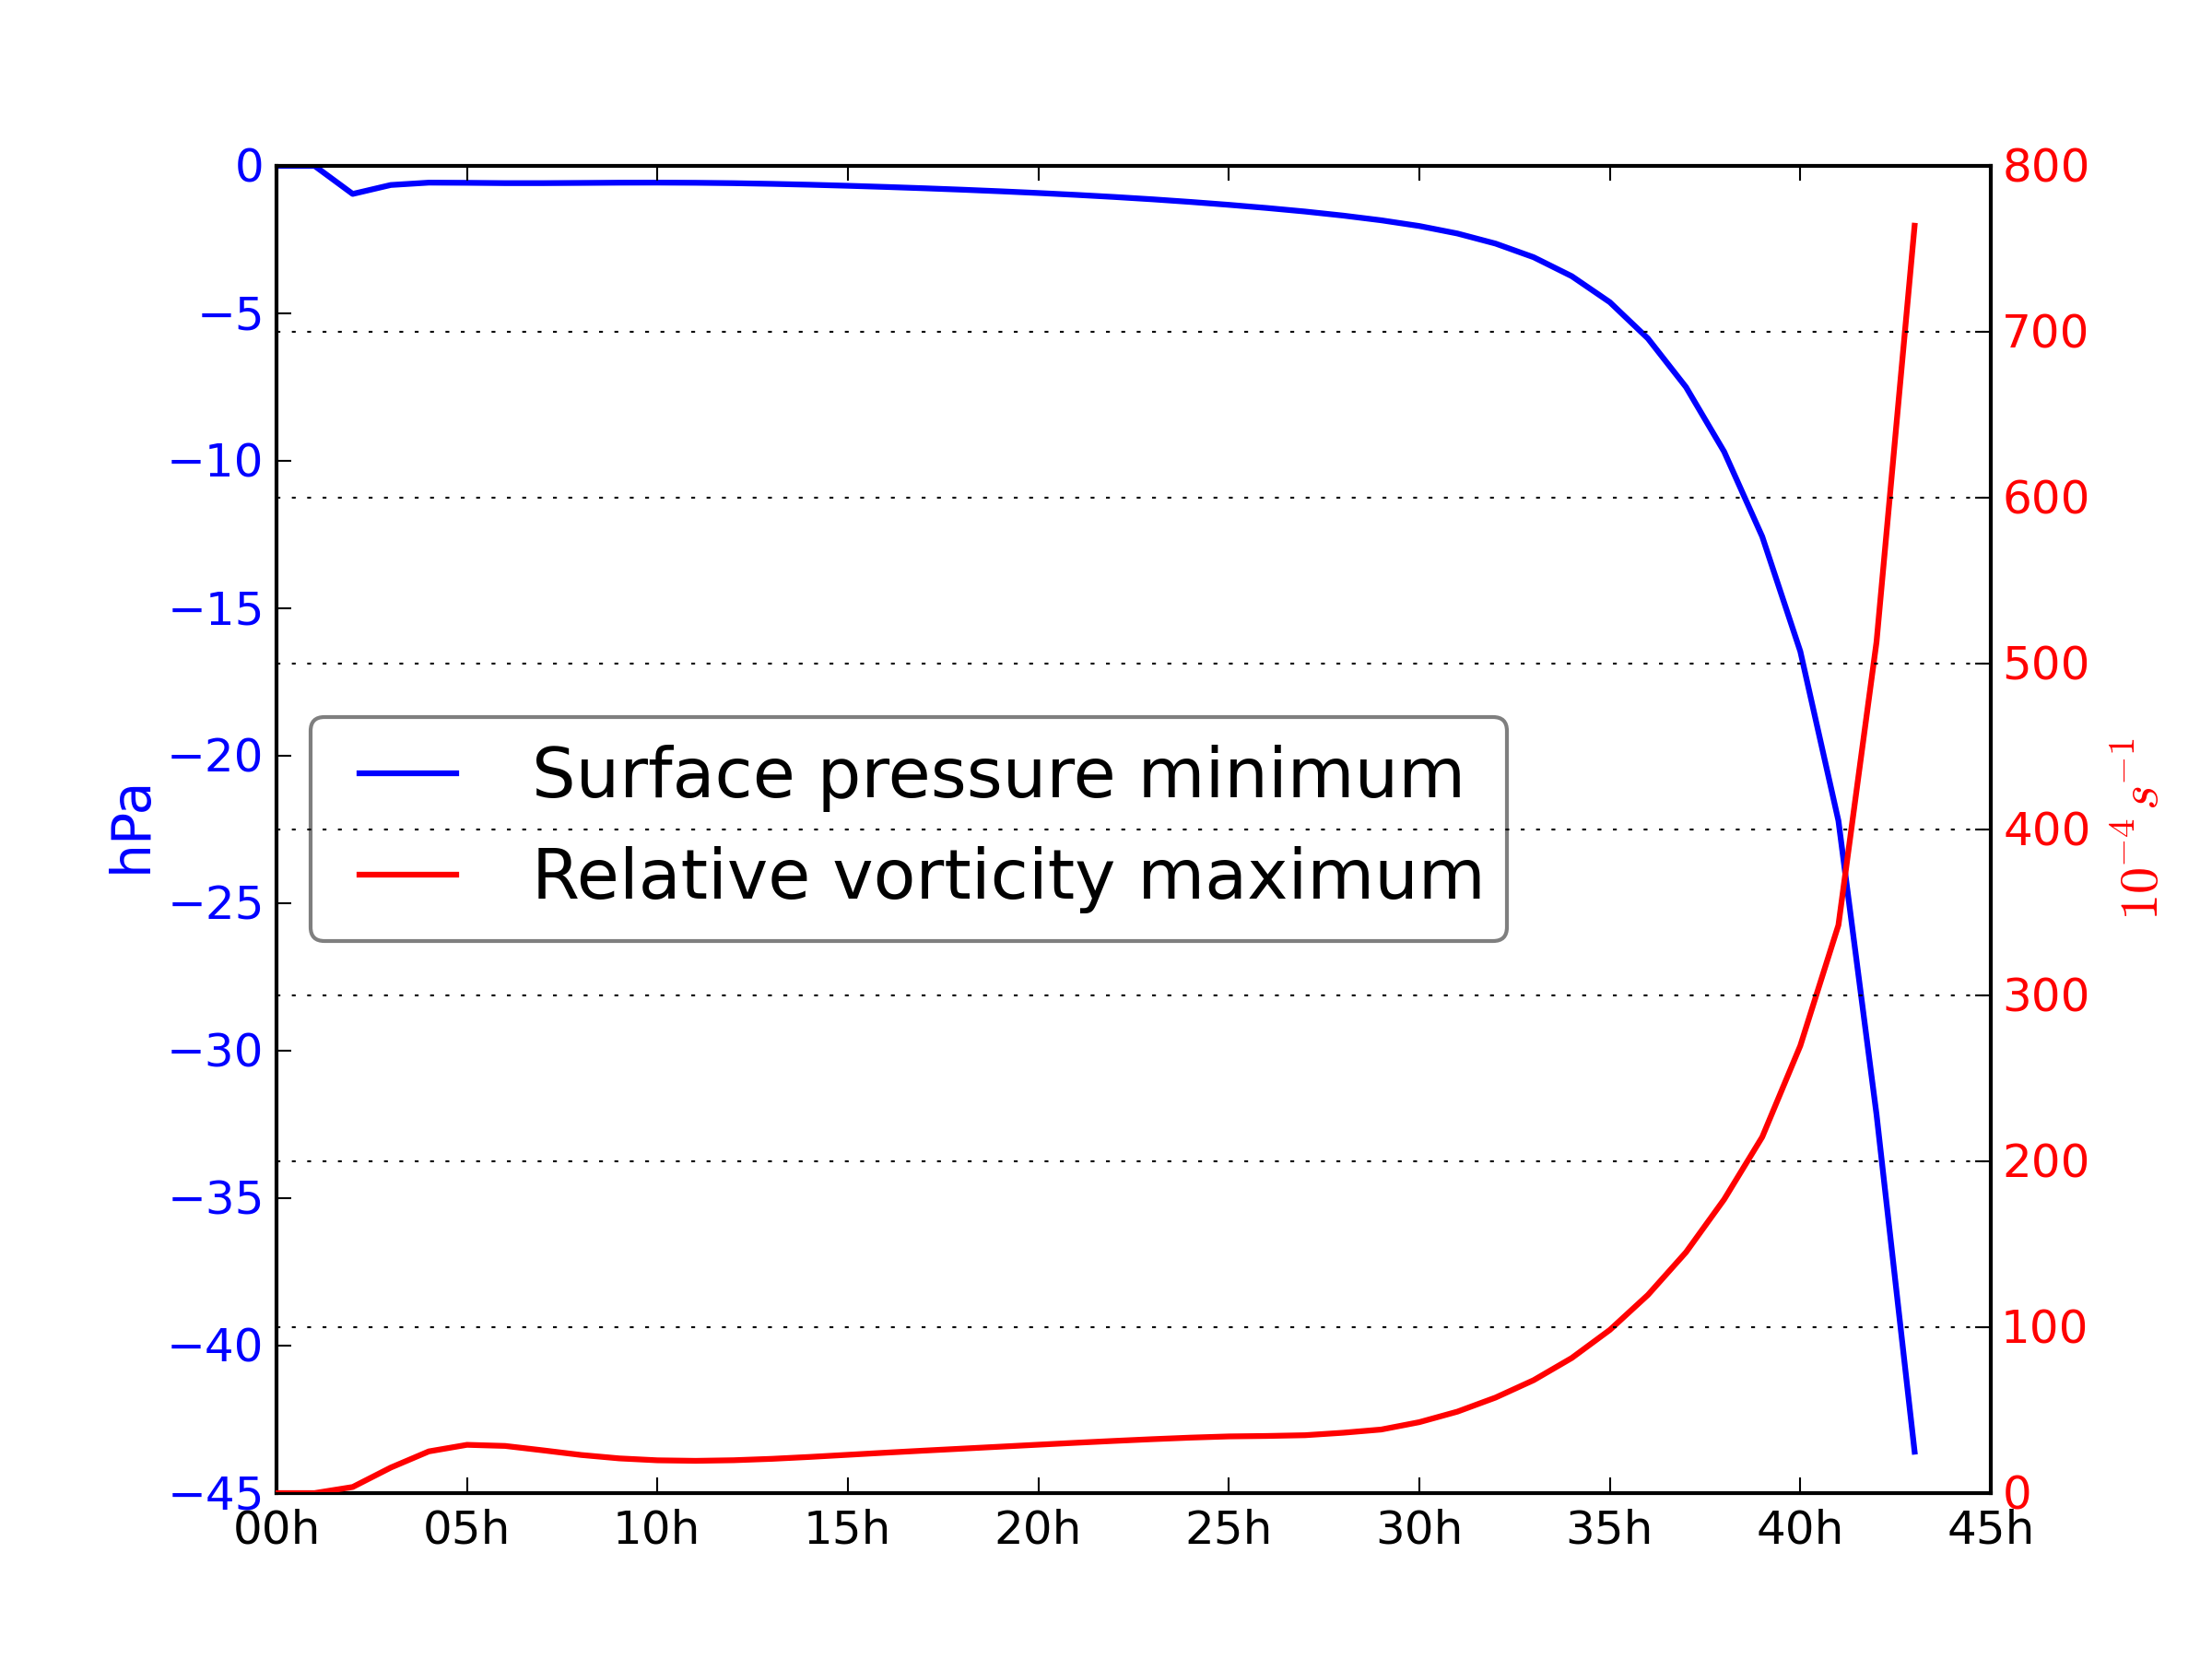
\includegraphics[width=\linewidth]{{./chapters/figures_results/slpmin_vortmax.00h-43h.ctrl}.png}
\end{center}
\caption{Изменение аномалии приземного давления и максимальной завихренности во времени. Эксперимент CTRL.}
\label{fig:ctrl_slpminvortmax}
\end{wrapfigure} 

Исходя из представленных графиков, можно заключить, что эволюция вихря происходила поступательно, без каких-либо смен режимов, за исключением испускания волн на начальной стадии. Из рис. \ref{fig:ctrl_slpminvortmax} также видно, что форма кривых изменения аномалии давления и максимума завихренности очень схожа, поэтому глубину циклона можно оценивать и первым, и вторым параметром \citep{YanaseEtAl2004}.

\subsection{Структура развитого вихря}
Для понимания механизма развития полярного мезоциклона логично остановиться на анализе его структуры в стадии достаточного развития, основываясь на горизонтальных и вертикальных разрезах полей метеовеличин за 36 час развития (12 часов вторых суток интегрирования), когда скорость приземного ветра превысила $15\mps$ (рис. \ref{fig:ctrl_hwind}).

Форма циклонического возмущения ожидаемо остается осесимметричной, в силу отсутствия фонового потока. Изначачально положительная температурная аномалия интенсифицируется: приблизительно в два раза увеличивается ее радиус (до $100\km$), а высота возрастает до $6\km$ (рис. \ref{fig:ctrl_ptdev_rz}). В соответствии с полем температуры находится и поле давления, аномалия которого у поверхности также достигает радиуса $100$--$120\km$. 

\begin{figure}[ht]
	\centering
	\begin{subfigure}[t]{0.45\textwidth}
		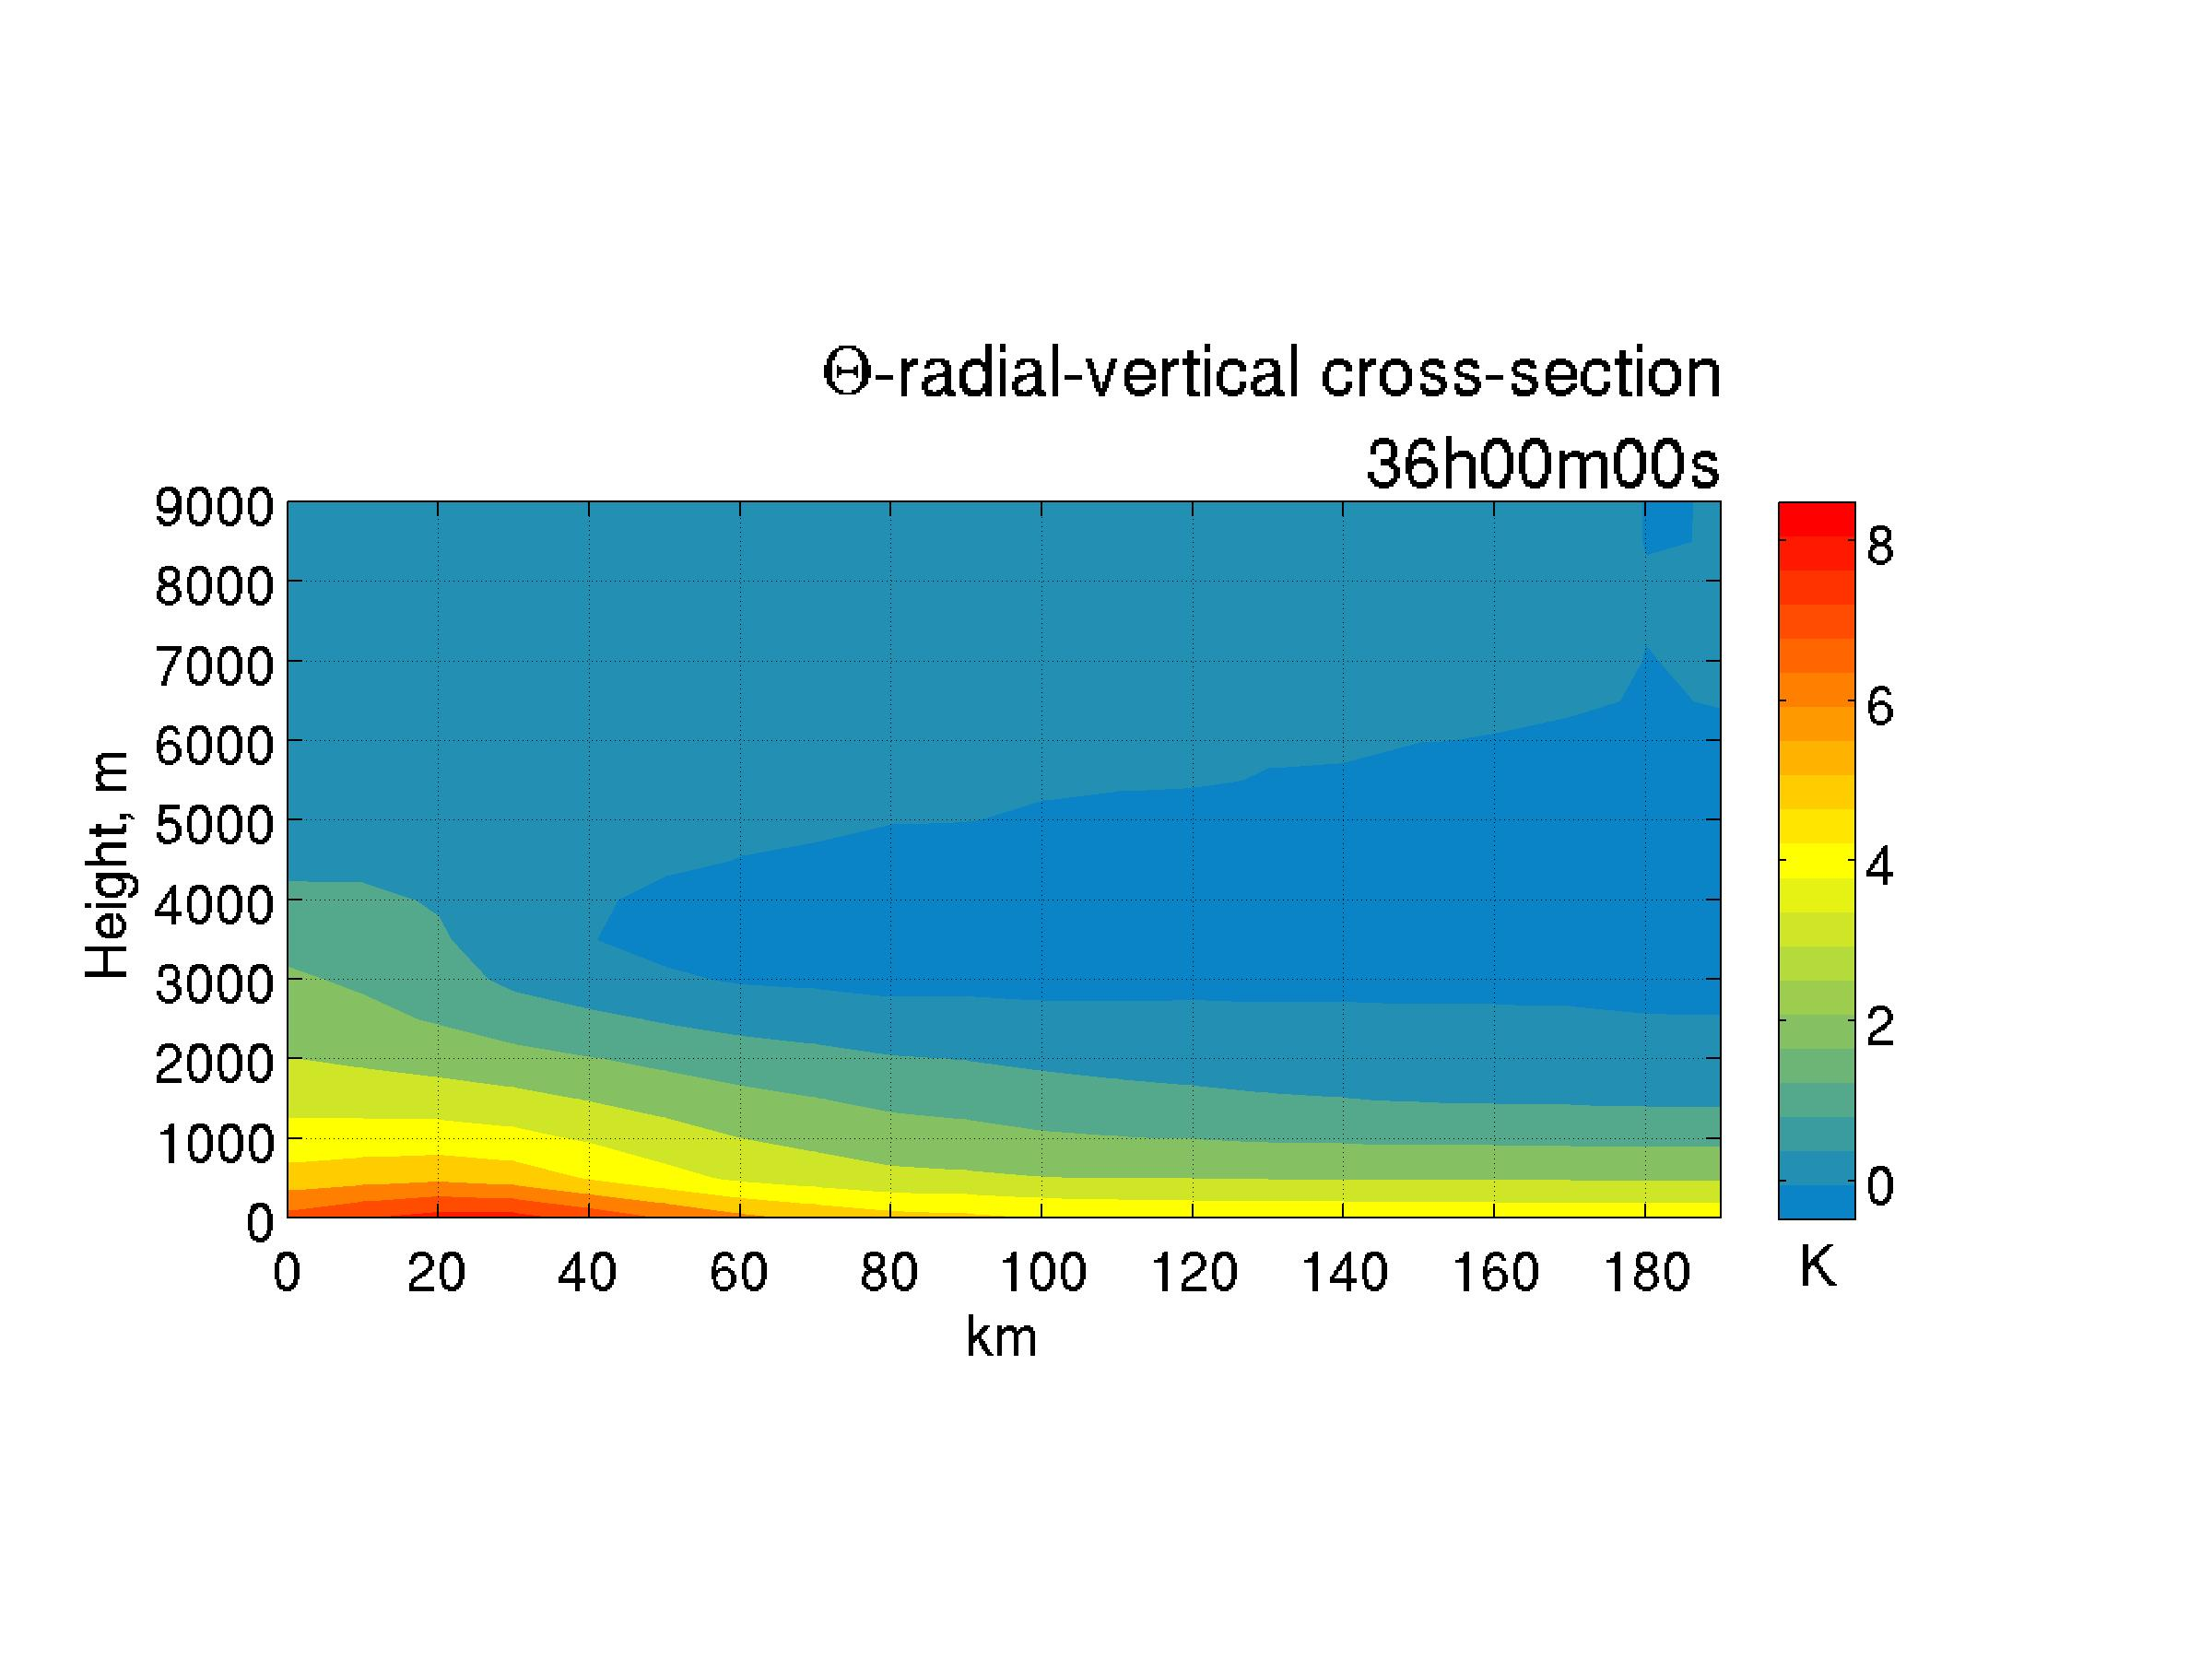
\includegraphics[width=\linewidth]{{./chapters/figures_results/ctrl_fields/ptdev_rz_z.ix52.360000}.jpg}
		\caption{Отклонения потенциальной температуры от фоновой ($\theta'$), $\K$.}
        \label{fig:ctrl_ptdev_rz}
	\end{subfigure}
	\hfill
	\begin{subfigure}[t]{0.45\textwidth}
		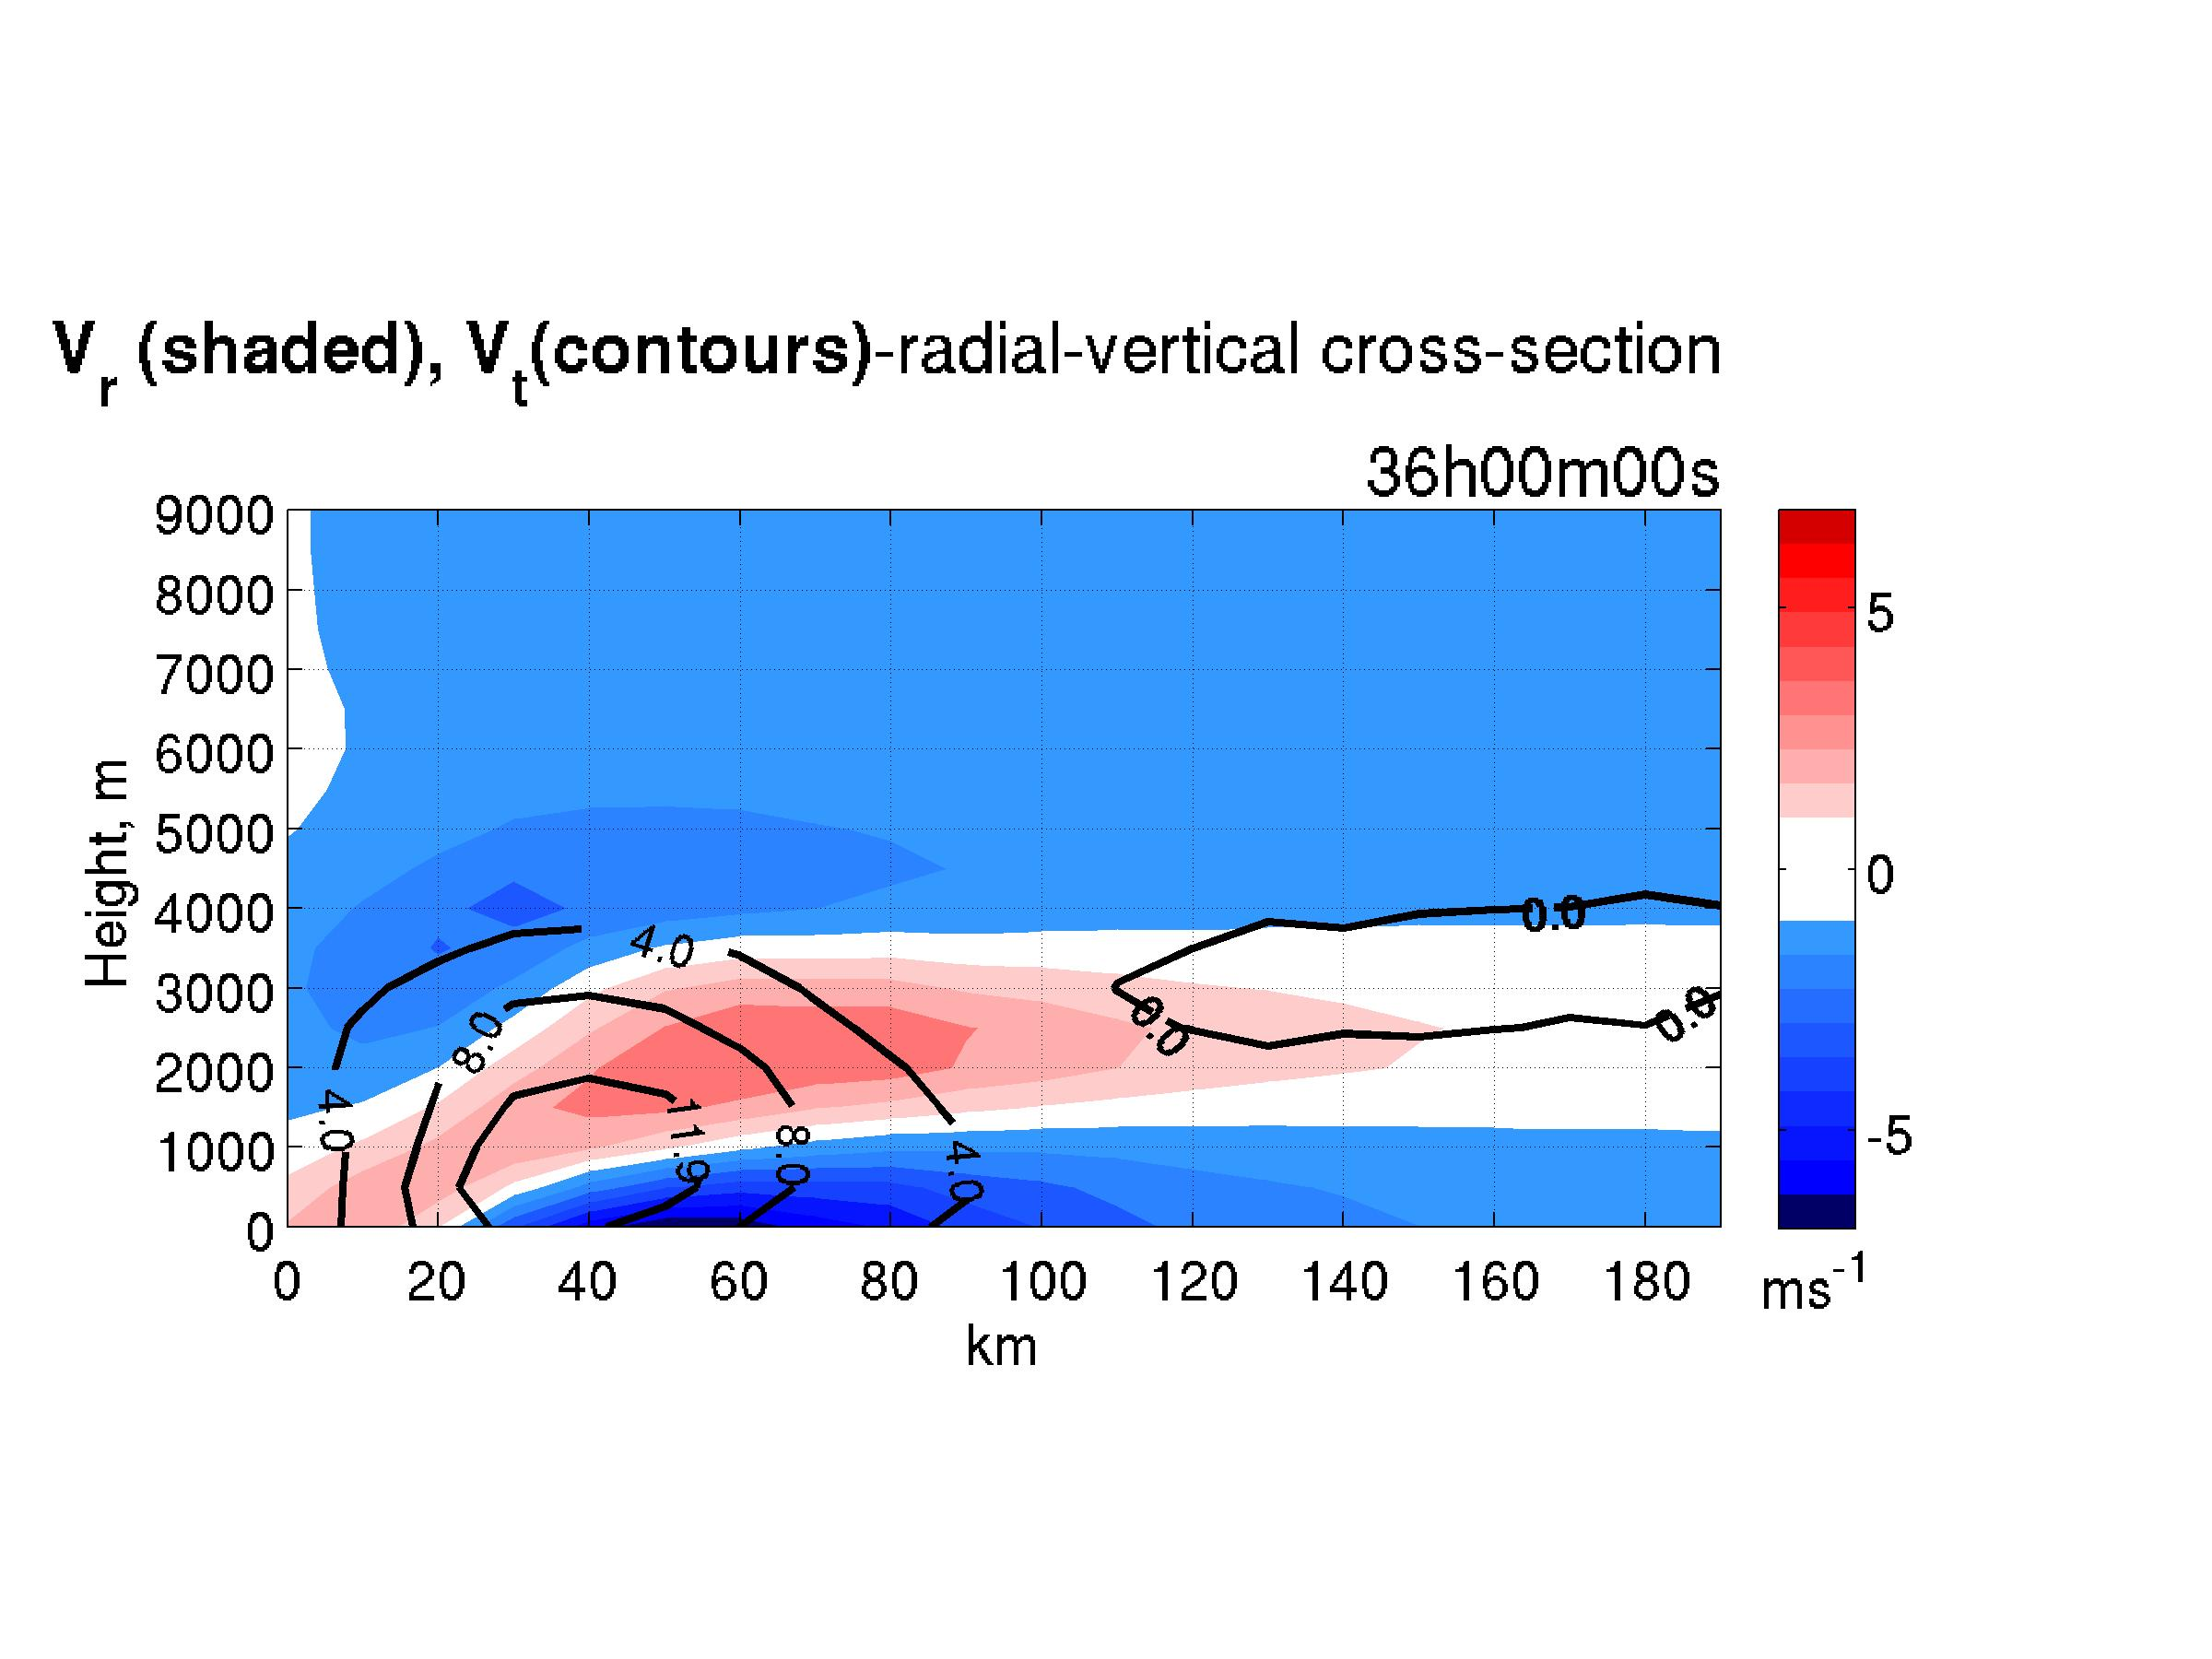
\includegraphics[width=\linewidth]{{./chapters/figures_results/ctrl_fields/vrvt_rz_z.ix52.360000}.jpg}
		\caption{Радиальная $v_r$ (цвет) и тангенциальная $v_t$ (контуры) компоненты скорости ветра, $\mps$.}
		\label{fig:ctrl_vrvt_rz}
	\end{subfigure}
	\hfill
    \begin{subfigure}[t]{0.45\textwidth}
		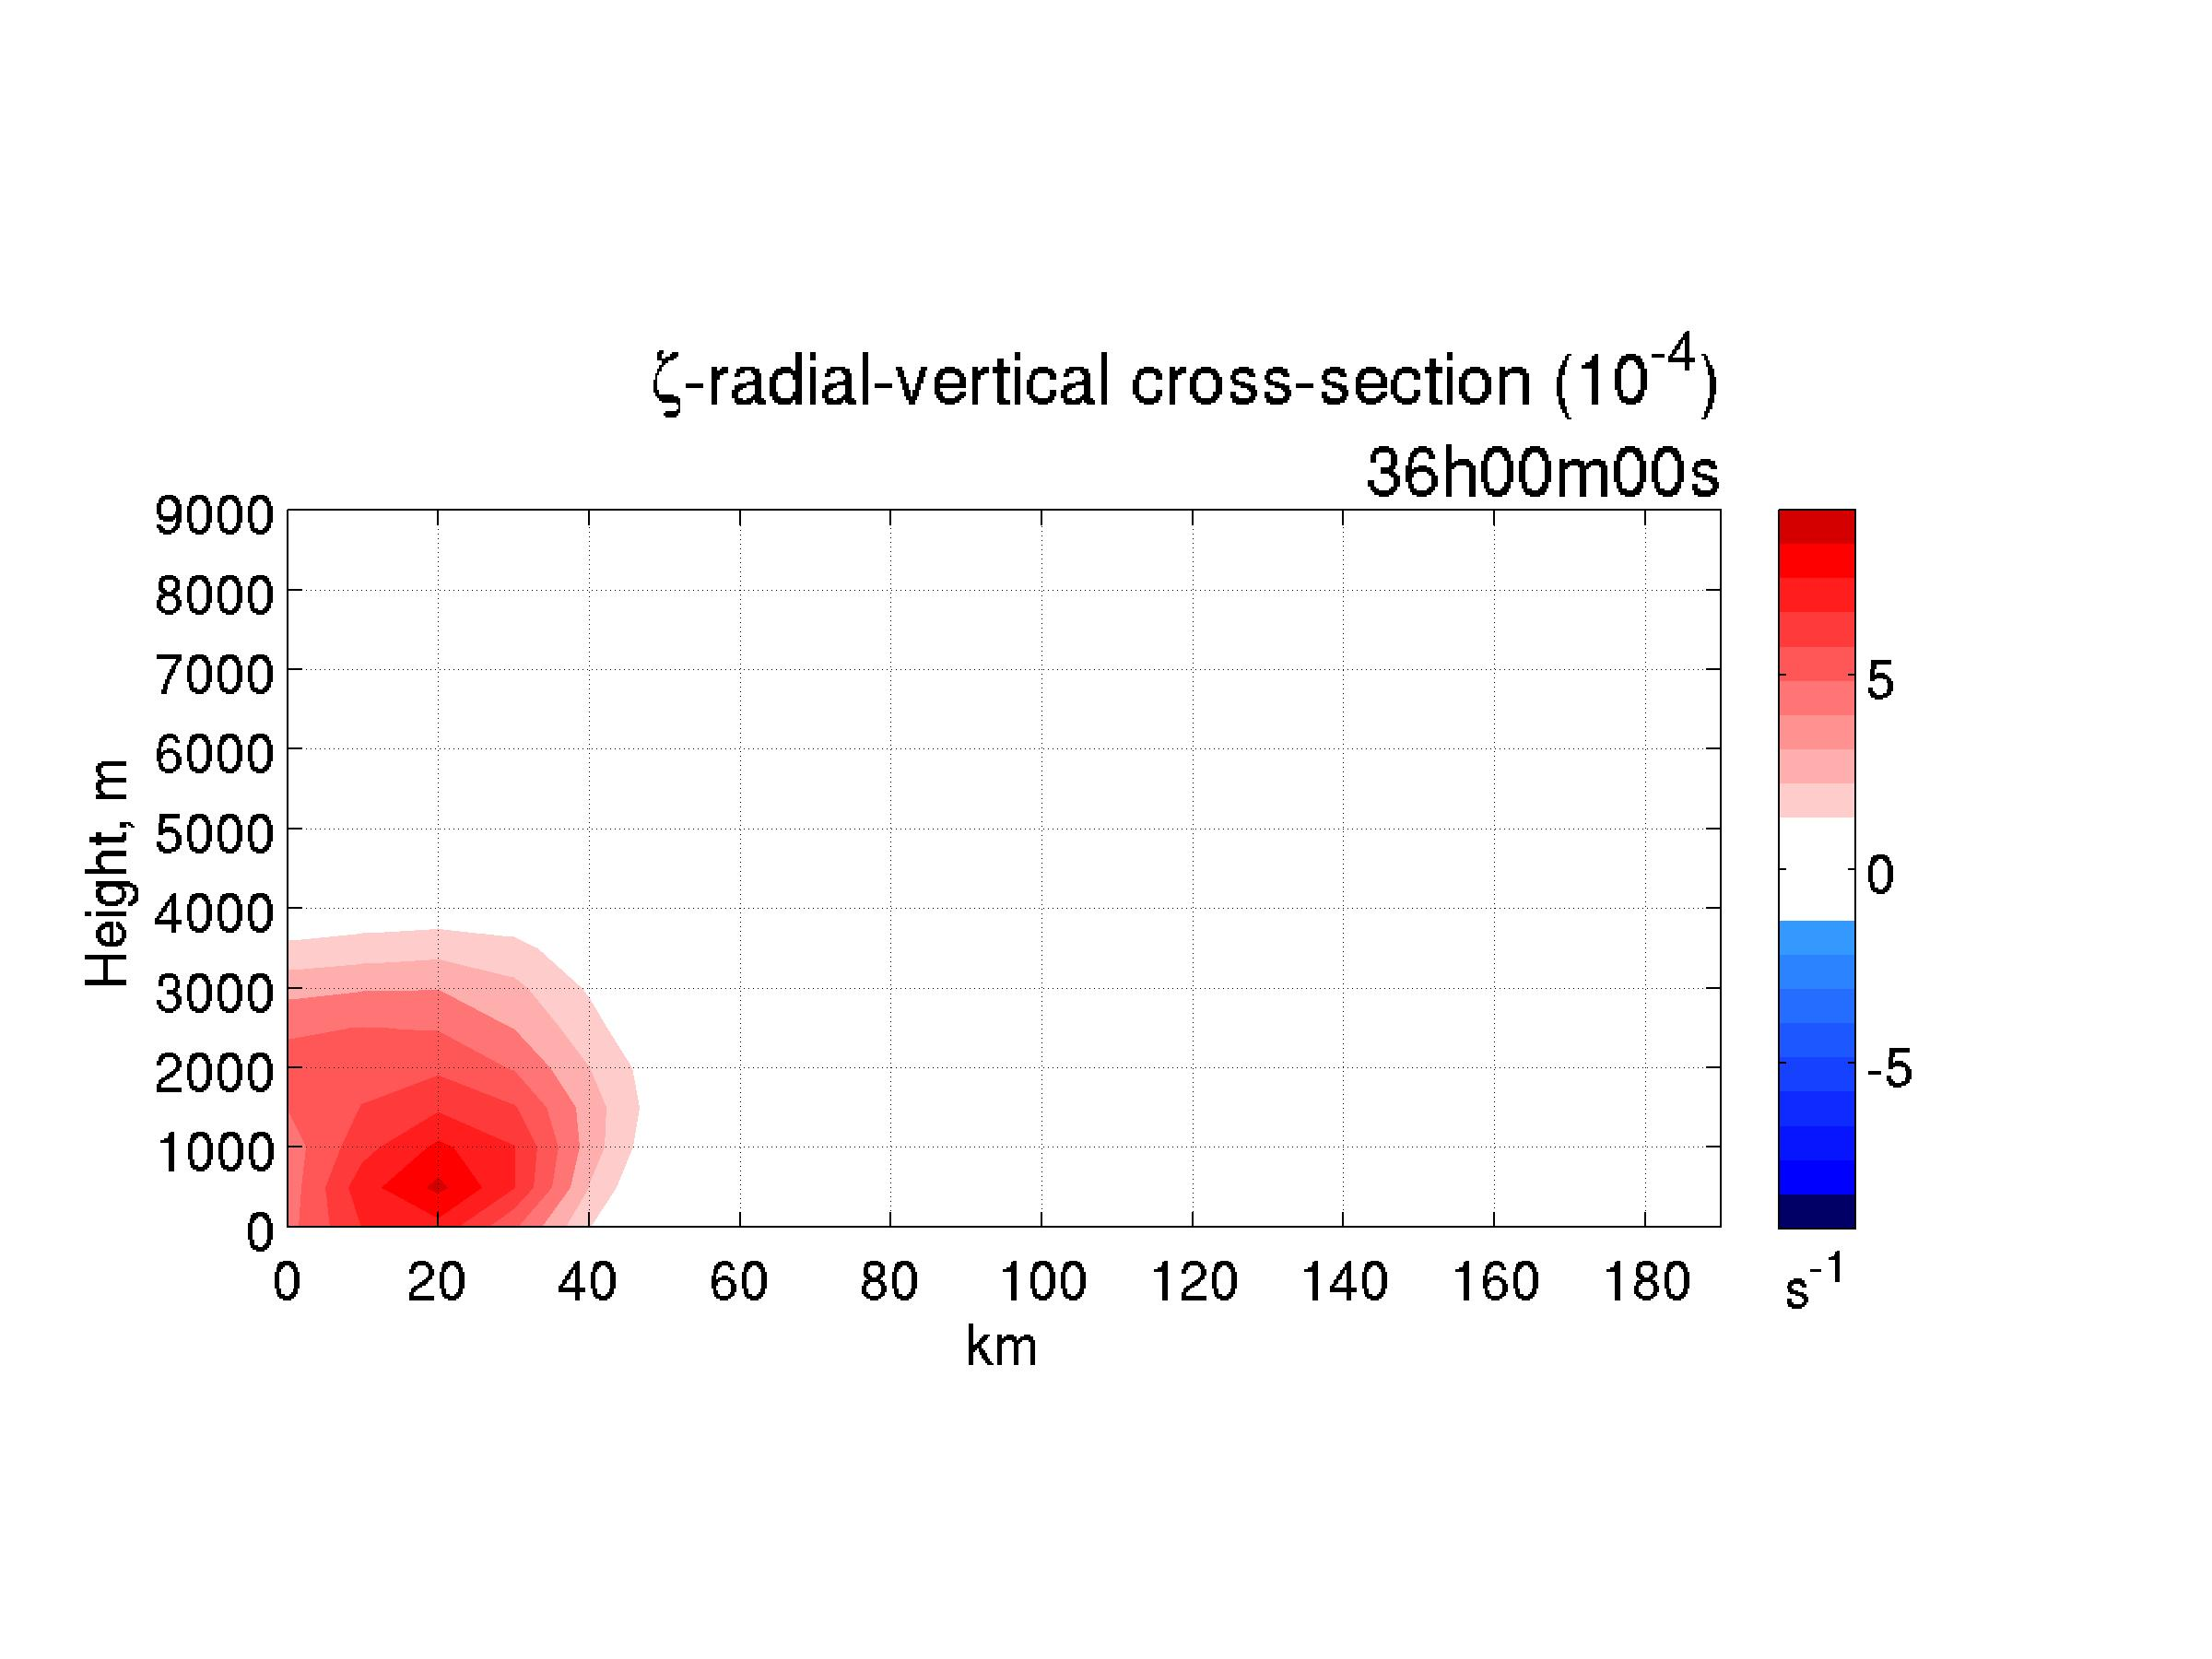
\includegraphics[width=\linewidth]{{./chapters/figures_results/ctrl_fields/vort_rz_z.ix52.360000}.jpg}
		\caption{Относительная завихренность ($\zeta$), $\pers$.}
		\label{fig:ctrl_vort_rz}
	\end{subfigure}
	\hfill
	\begin{subfigure}[t]{0.45\textwidth}
		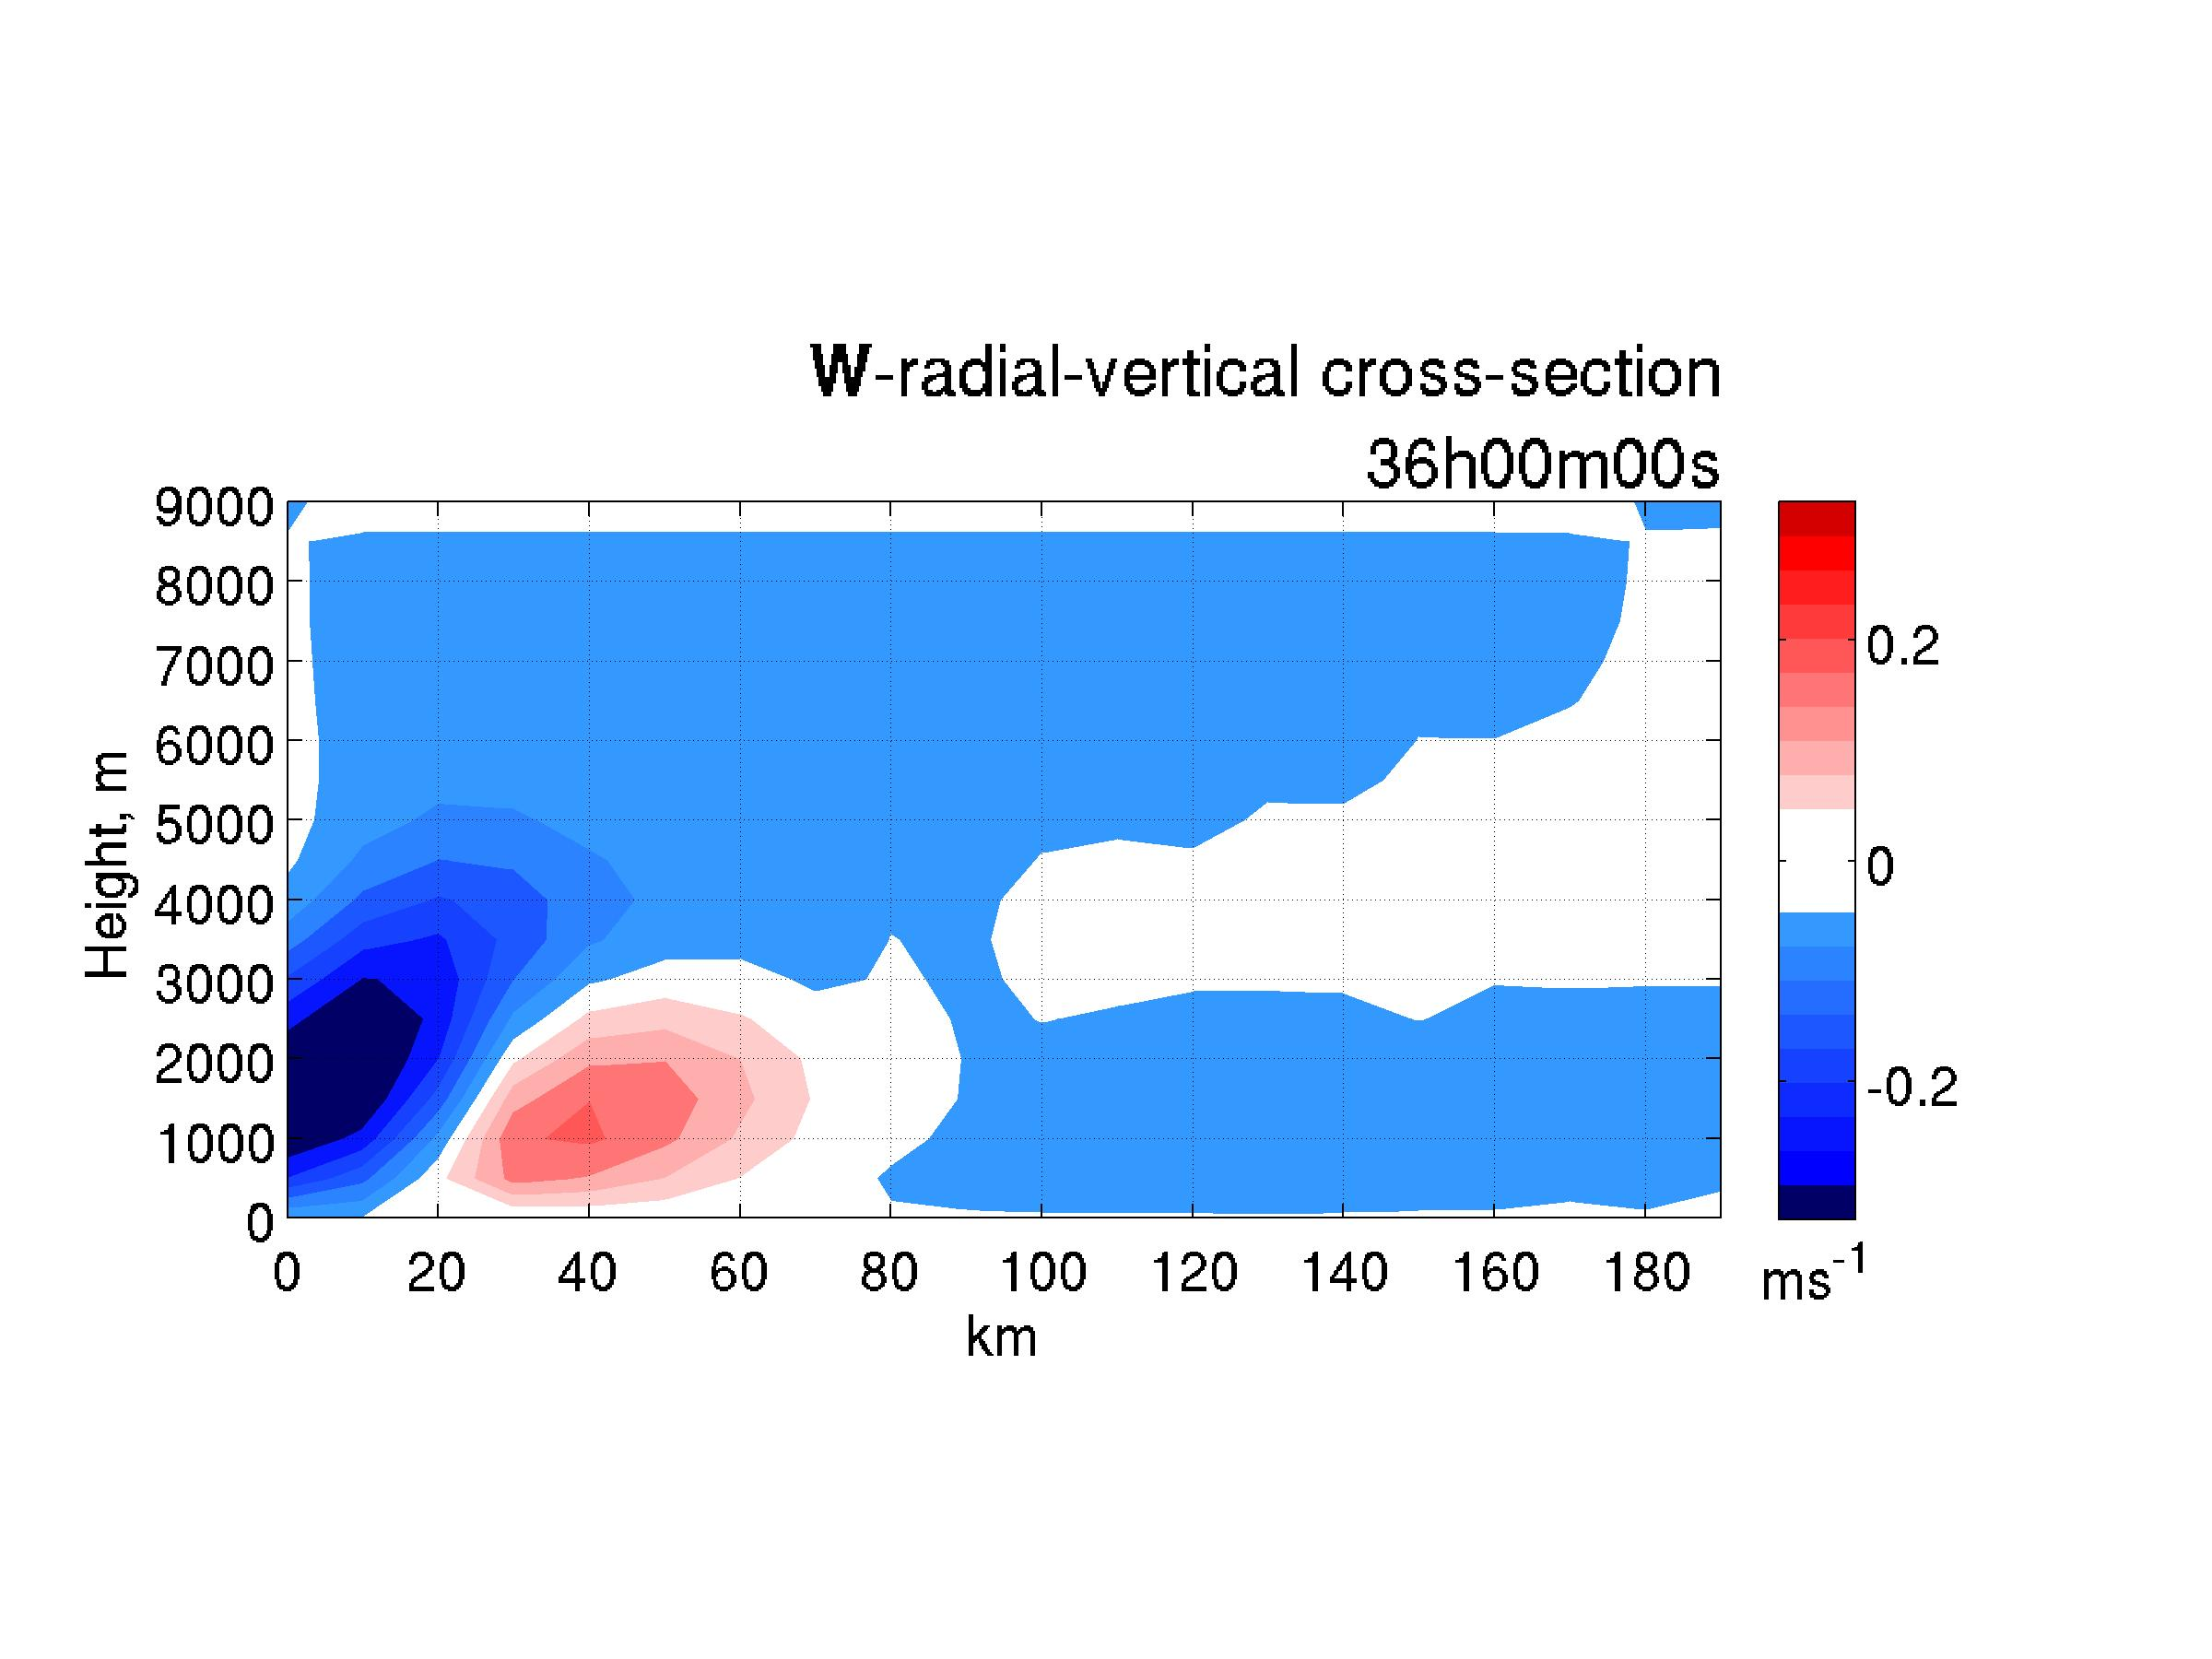
\includegraphics[width=\linewidth]{{./chapters/figures_results/ctrl_fields/w_rz_z.ix52.360000}.jpg}
		\caption{Вертикальная компонента скорости ветра ($w$), $\mps$.}
		\label{fig:ctrl_w_rz}
	\end{subfigure}
	\hfill
	\begin{subfigure}[t]{0.45\textwidth}
		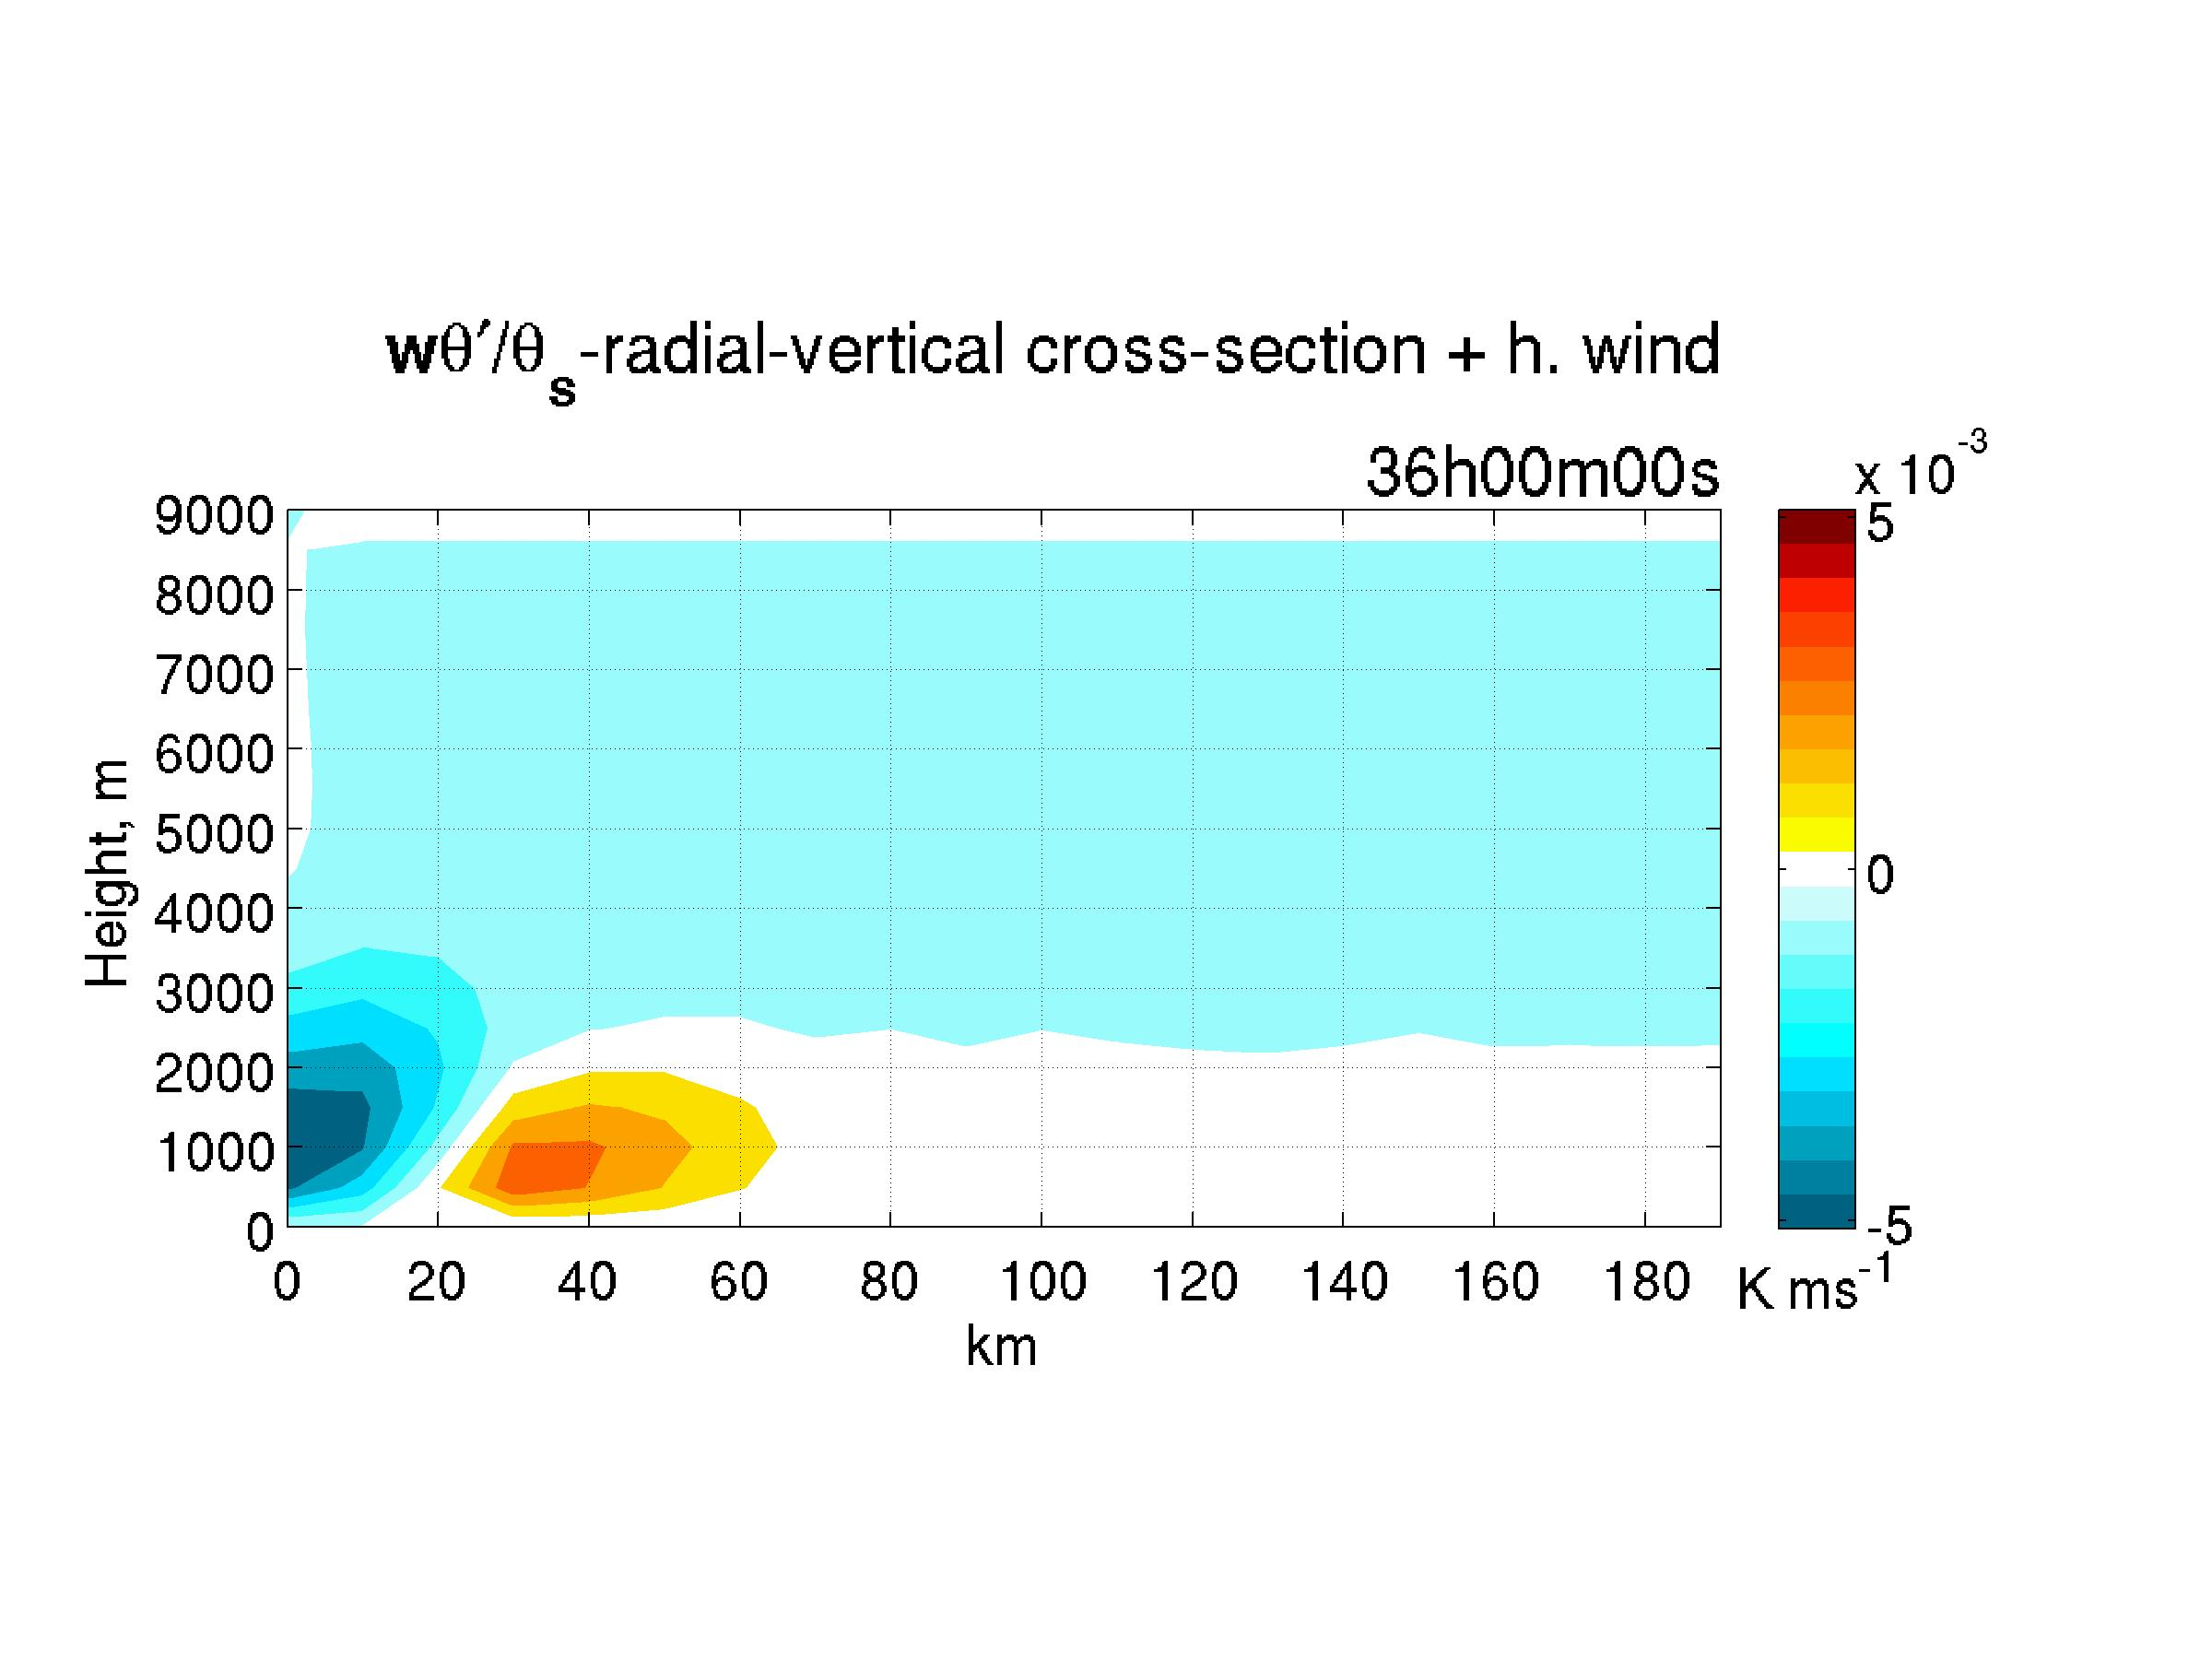
\includegraphics[width=\linewidth]{{./chapters/figures_results/ctrl_fields/buoyterm_rz_z.ix52.360000}.jpg}
		\caption{Поток силы плавучести ($w\theta'/\theta_s$), $\mps$.}
		\label{fig:ctrl_buoy_rz}
	\end{subfigure}
	\hfill
	\begin{subfigure}[t]{0.45\textwidth}
		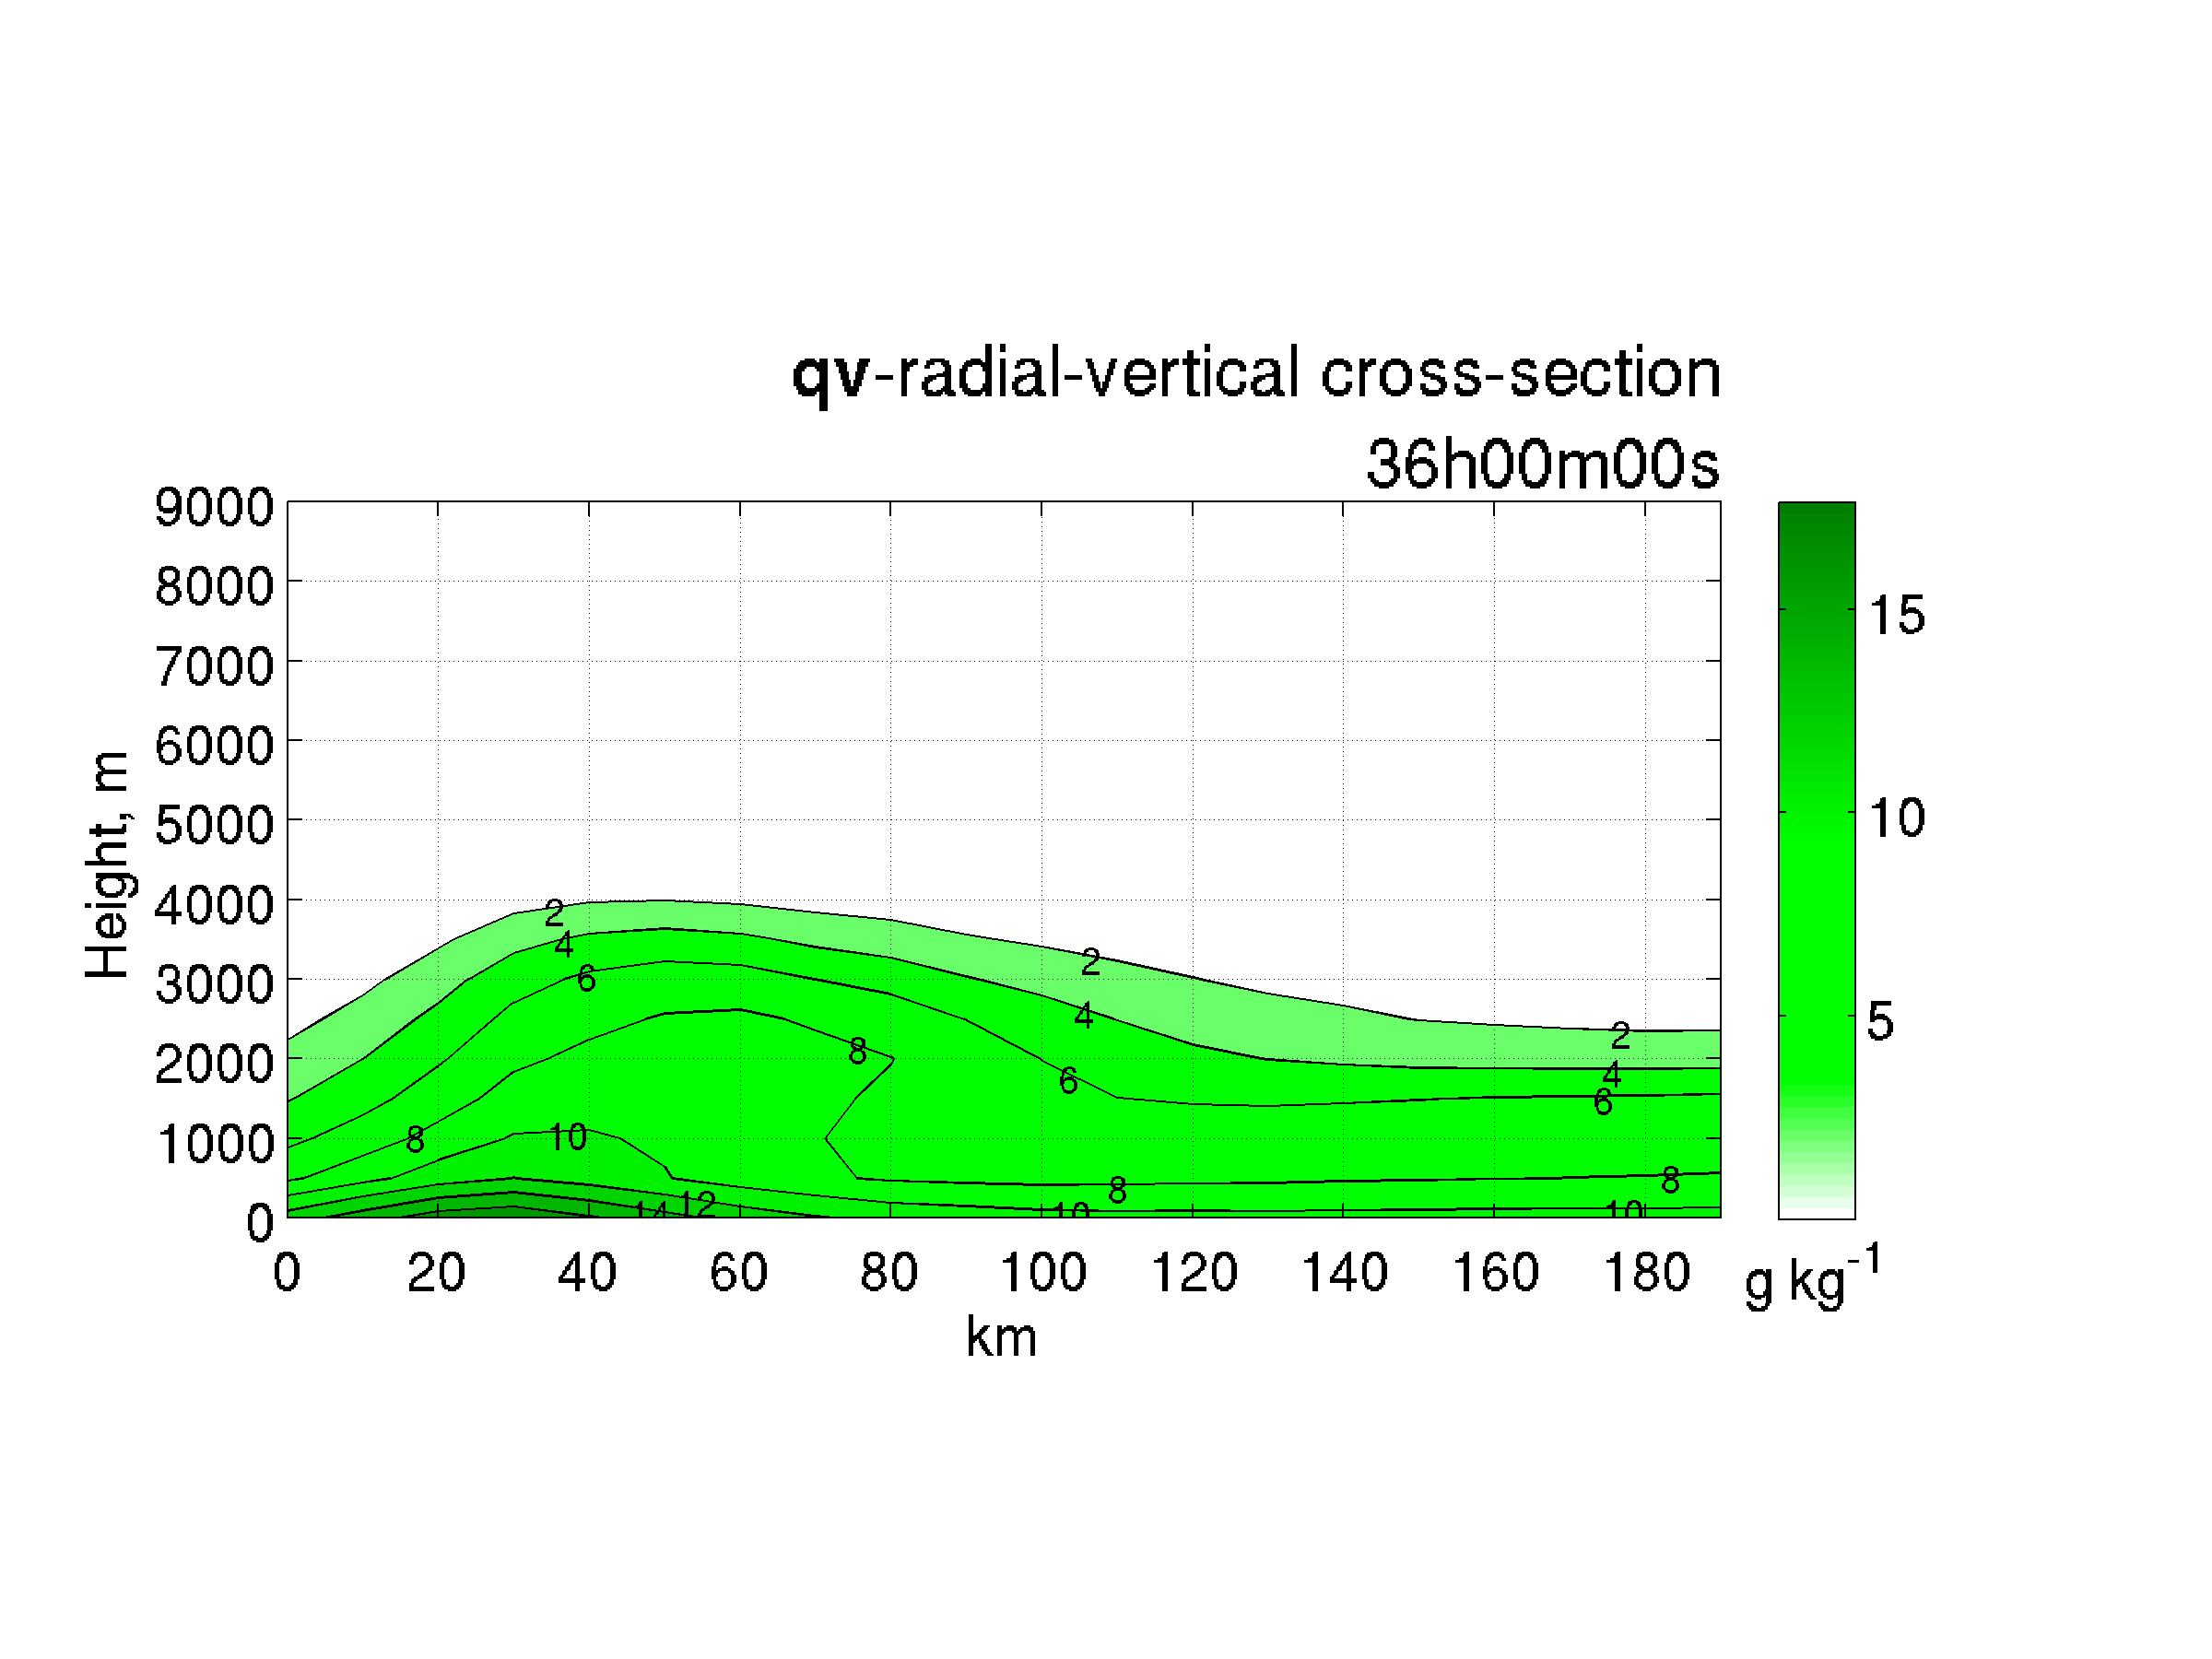
\includegraphics[width=\linewidth]{{./chapters/figures_results/ctrl_fields/qv_rz_z.ix52.360000}.jpg}
		\caption{Удельная влажность ($q_v$), $\gpkg$.}
		\label{fig:ctrl_qv_rz}
	\end{subfigure}
    \caption{Радиально-вертикальные разрезы. По оси абсцисс отложен радиус, $\km$, по оси ординат --- высота, $\m$. Эксперимент CTRL. 36 час модельного времени.}
\end{figure}

Под действием силы барического градиента в центре области возникает конвергенция скорости, которая под действием силы вращения Земли приобретает циклоническую завихренность (\ref{fig:ctrl_vort_rz}). Адекватность воспроизведения моделью этого фундаментального явления было проверено в дополнительном эксперименте с отключенным ускорением Кориолиса в уравнении движения (\ref{eq:progn1,eq:progn2}). Как видно из рис. \ref{fig:ctrl_vrvt_rz}, где изображены радиальная и азимутальная (тангенциальная) скорости, в стадии развитого вихря конвергенция сосредоточена ниже $1000\m$ на расстоянии от $40$ до $120\km$ с максимумом вблизи земной поверхности и на радиусе $50\km$. Внутреннюю часть этой зоны обозначим как глаз циклона в соответствии с терминологией тропических циклонов. Выше зоны конвергенции находится менее интенсивная область оттока воздуха, характеризующаяся положительной радиальной скоростью.

На рис. \ref{fig:ctrl_vrvt_rz} черным цветом показаны изолинии азимутальной скорости движения воздуха в вихре. Максимум циклонического азимутального ветра находится на уровне нулевой радиальной скорости ($500$--$1000\m$) и составляет $11.9\mps$, а радиус максимальных значений равняется около $40\km$ (радиус максимального ветра, РМВ). Существовавший в начальные этапы развития циклона слабый высотный антициклон уже не виден в 36 час модельного времени. Глазу циклона соответствует область малых скоростей ветра. Заметим, что глаз вихря оказывается слишком малым в поперечнике, чем обычно характерно для полярных мезоциклонов (\citep{CraigGray1996}).

Радиальный разрез вертикальной скорости виден на рис. \ref{fig:ctrl_w_rz}. Распределение этой компоненты ветра таково, что область положительных значений находится на расстоянии $20$--$70\km$ от центра циклона и наклонена \emph{от} центра. То есть область $w>0$ совпадает с областью максимальных ветров. Восходящие движения наиболее сильны в слое $1000$--$1500\m$ над поверхностью, где $w$ достигает $0.2\mps$. Отрицательные значения вертикальной скорости наблюдаются в области глаза циклона, и по амплитуде превосходят положительные в $\approx 1.5$ раза. 

Относительная завихренность в нижних слоях атмосферы распределена симметрично относительно центра циклона, причем максимум, уже на порядок превосходящий параметр Кориолиса, наблюдается на расстоянии около $25\km$ от центра. Среди членов, определяющих  изменение завихренности наибольшую величину имеет слагаемое растяжения (\ref{fig:ctrl_stretch36}), причем положительные значения находятся на периферии циклона ($\approx 2\times 10^{-7}\s^{-2}$), а отрицательные --- в центре. Таким образом, проявляется тенденция к расширению циклона и концентрации количества движения на кольце максимальных ветров. Вторым по значимости в бюджете завихренности является слагаемое горизонтальной адвекции (порядка $10^{-7}$), у которого преобладают отрицательные значения, несколько компенсируя дивергентное слагаемое на внешнем радиусе циклона. Два остальных компонента бюджета завихренности имеют значения одного порядка ($10^{-8}$), но действуют противоположно: слагаемое вертикальной адвекции имеет отрицательные значения в рассматриваемом районе, а слагаемое наклона положительно.

\begin{figure}[t]
	\centering
	\begin{subfigure}[t]{0.45\textwidth}
		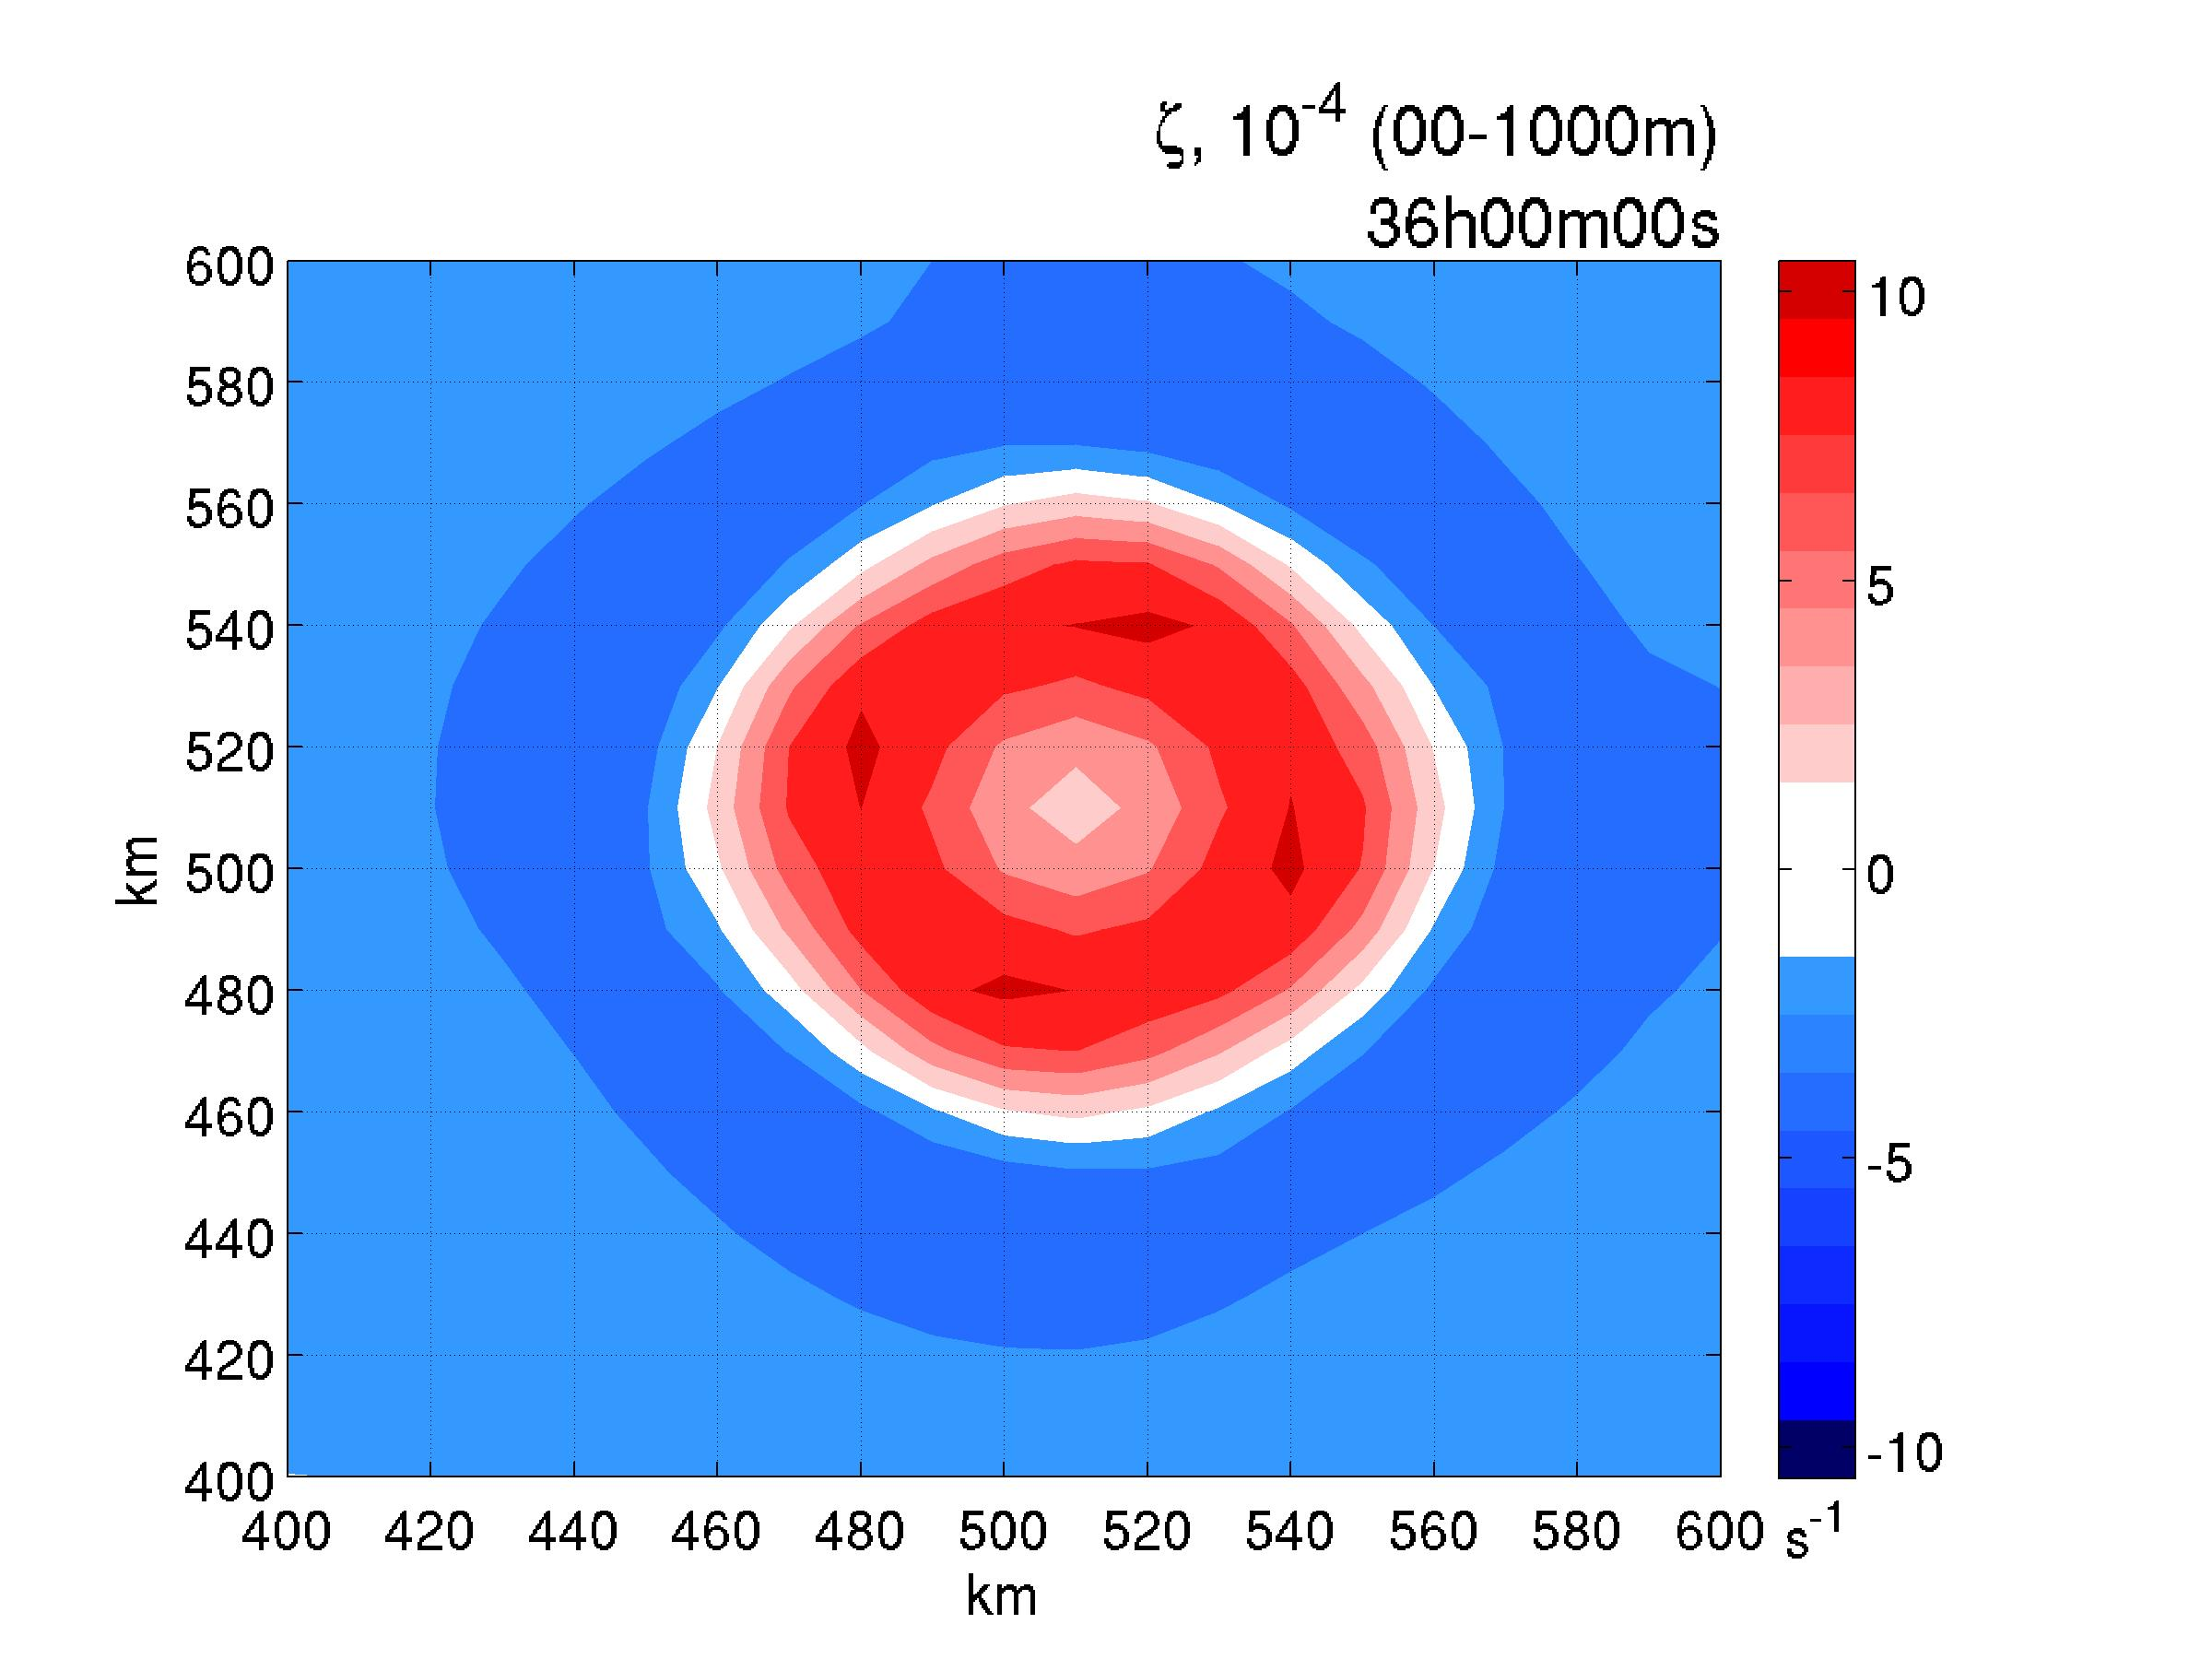
\includegraphics[width=\linewidth]{{./chapters/figures_results/ctrl_fields/rot_z_z.x41-x61.y41-y61.ilev02.360000}.jpg}
		\caption{ }
        \label{fig:ctrl_rotz36}
	\end{subfigure}
	\hfill
	\begin{subfigure}[t]{0.45\textwidth}
		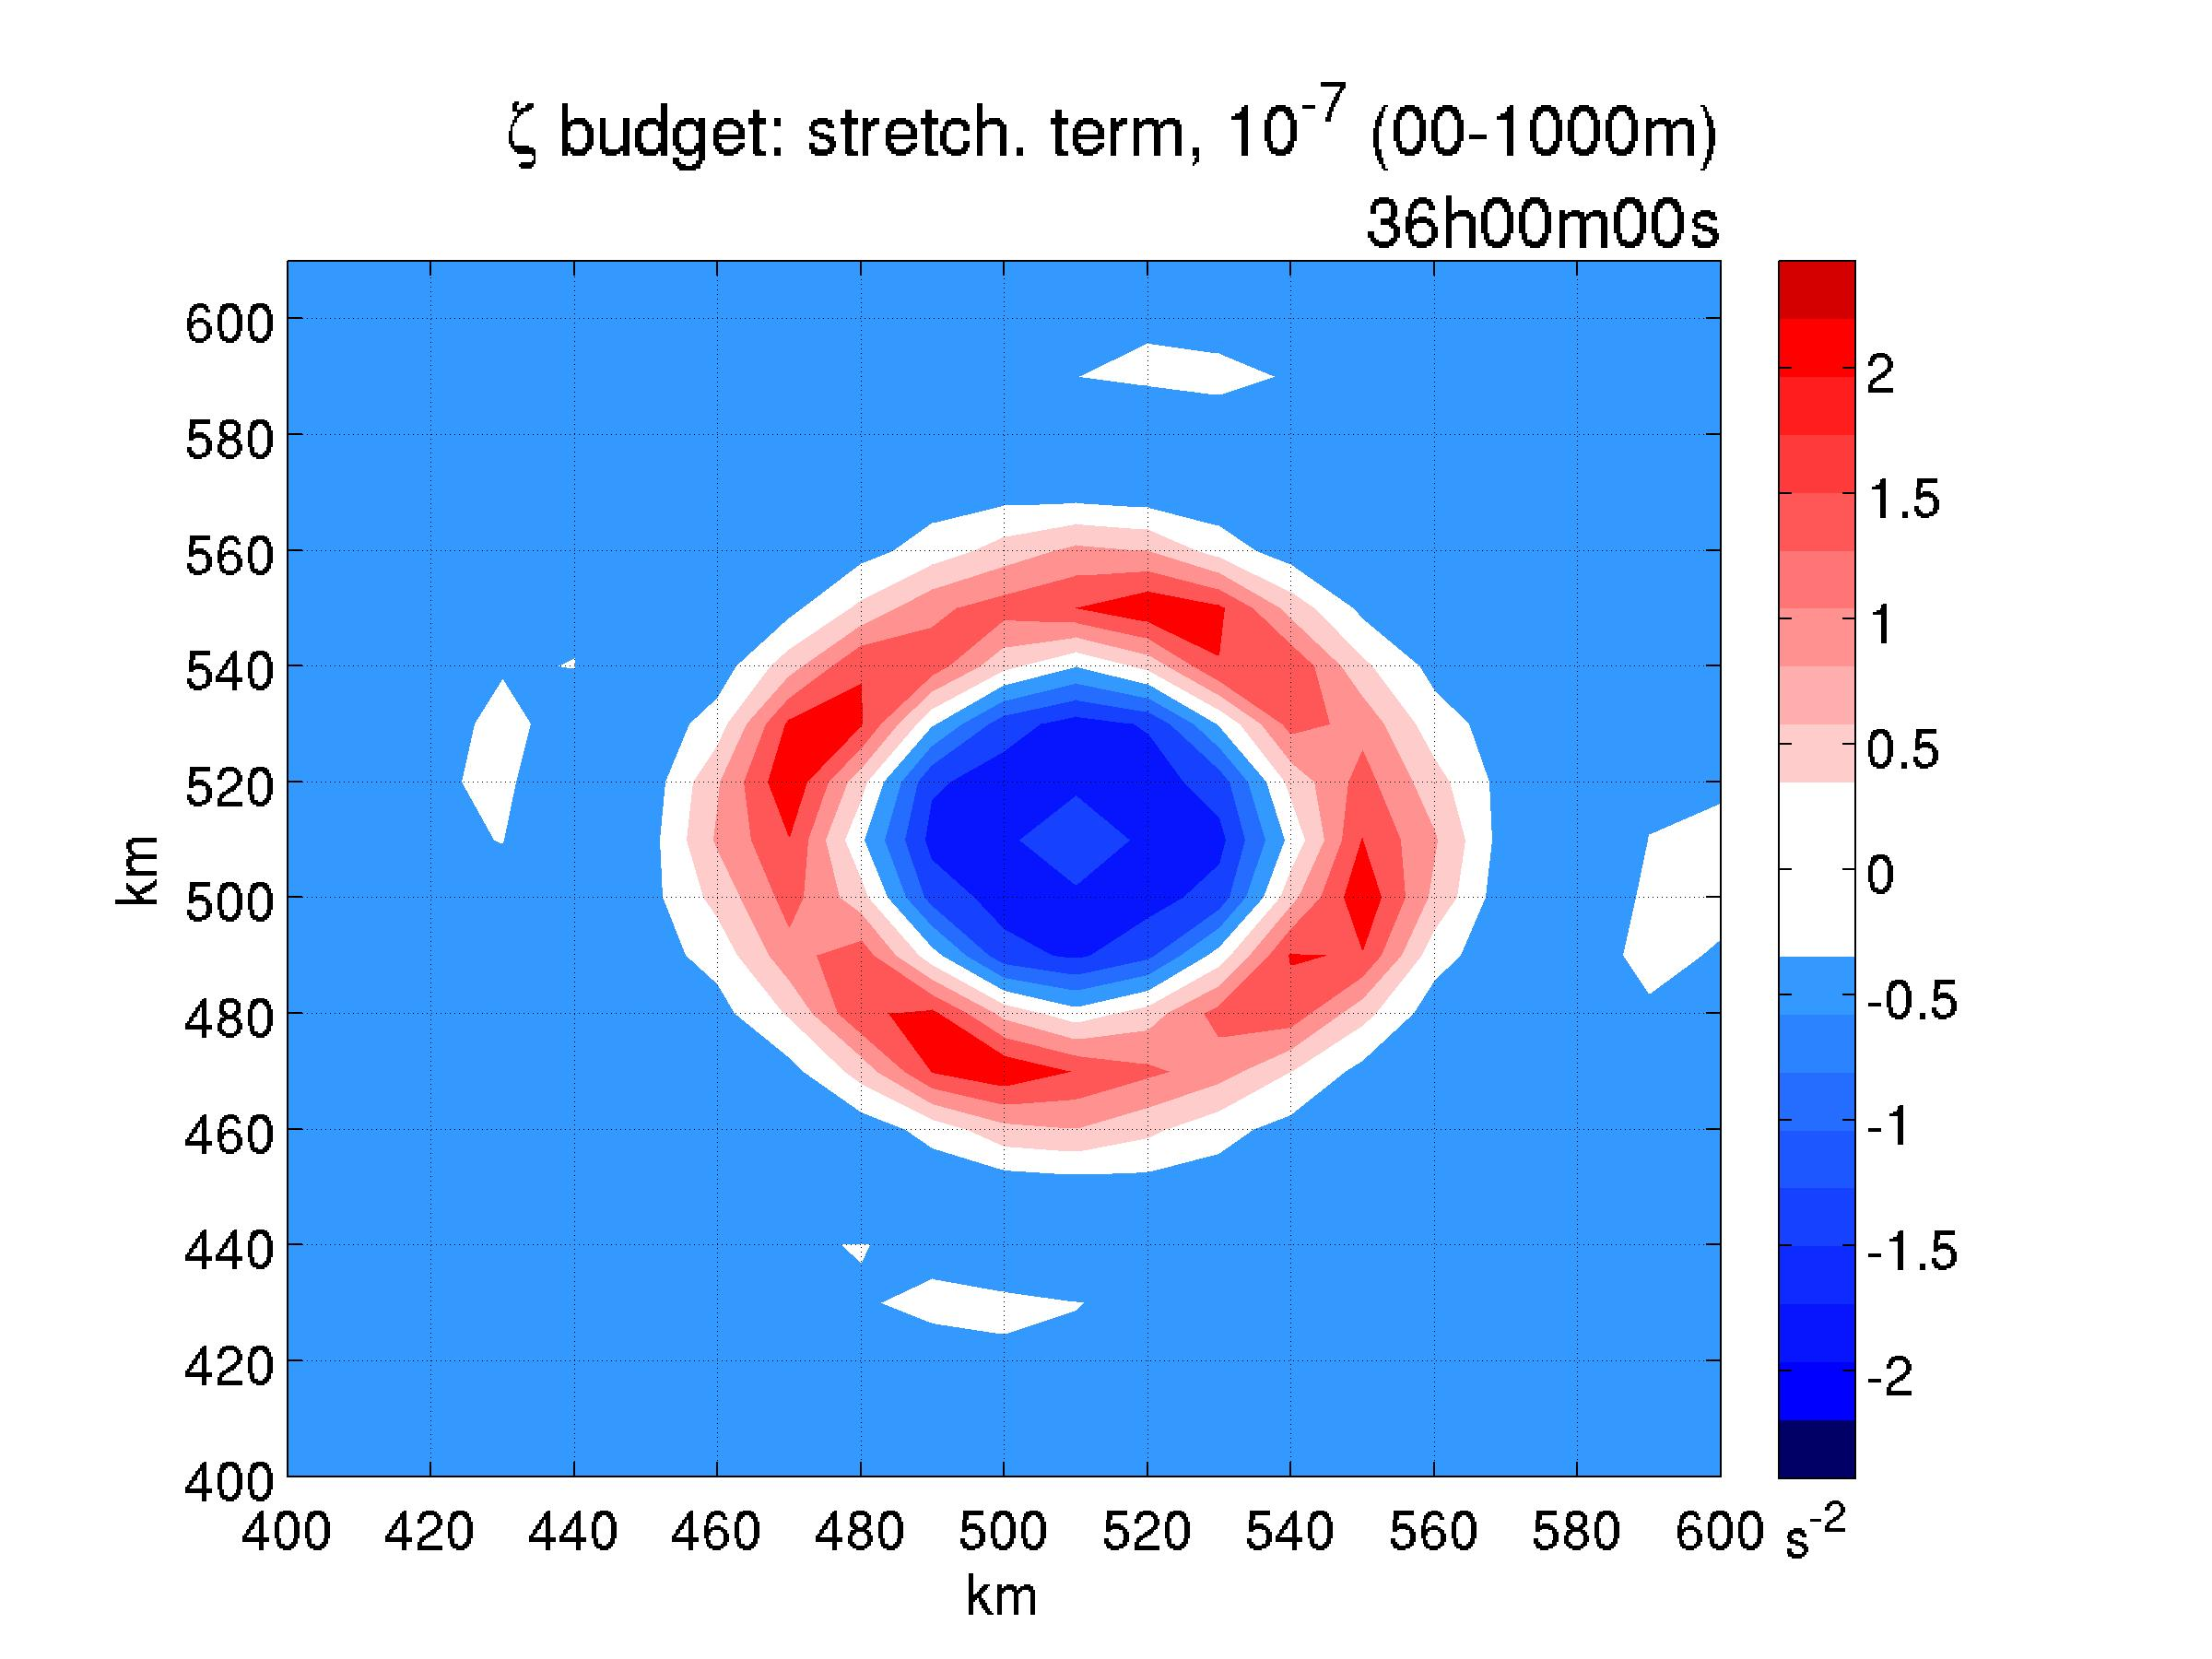
\includegraphics[width=\linewidth]{{./chapters/figures_results/ctrl_fields/vort_budget_stretch_z.x41-x62.y41-y61.ilev02.360000}.jpg}
		\caption{ }
		\label{fig:ctrl_stretch36}
	\end{subfigure}
    \caption{Поле относительной завихренности ($\zeta$) и слагаемое растяжения (\ref{eq:vorttend}) бюджета завихренности, осредненные в слое ниже $1000\m$. Эксперимент CTRL. 36 час модельного времени.}
\end{figure}

Развившийся вихрь находится в сбалансированном состоянии: правая и левая части в уравнении градиентного баланса (в котором слагаемое центростремительного ускорения превышает ускорение Кориолиса почти в 2 раза) очень близки по величине. Это также подтверждается рис. \ref{fig:grwindbal}.

\subsection{Разделение вихря}
Моделируемый мезоциклон достигает больших скоростей к концу вторых суток интегрирования, что вызывает численную неустойчивость эксперимента. При этом наблюдается разделение вихря на две отдельные циклонические депрессии (рис. \ref{fig:ctrl_split_hwind}), которые продолжают усиливаться, и в последний час эксперимента максимальная скорость ветра в нижней атмосфере превышает $80\mps$. 

\begin{wrapfigure}{L}{0.5\textwidth}
\begin{center}
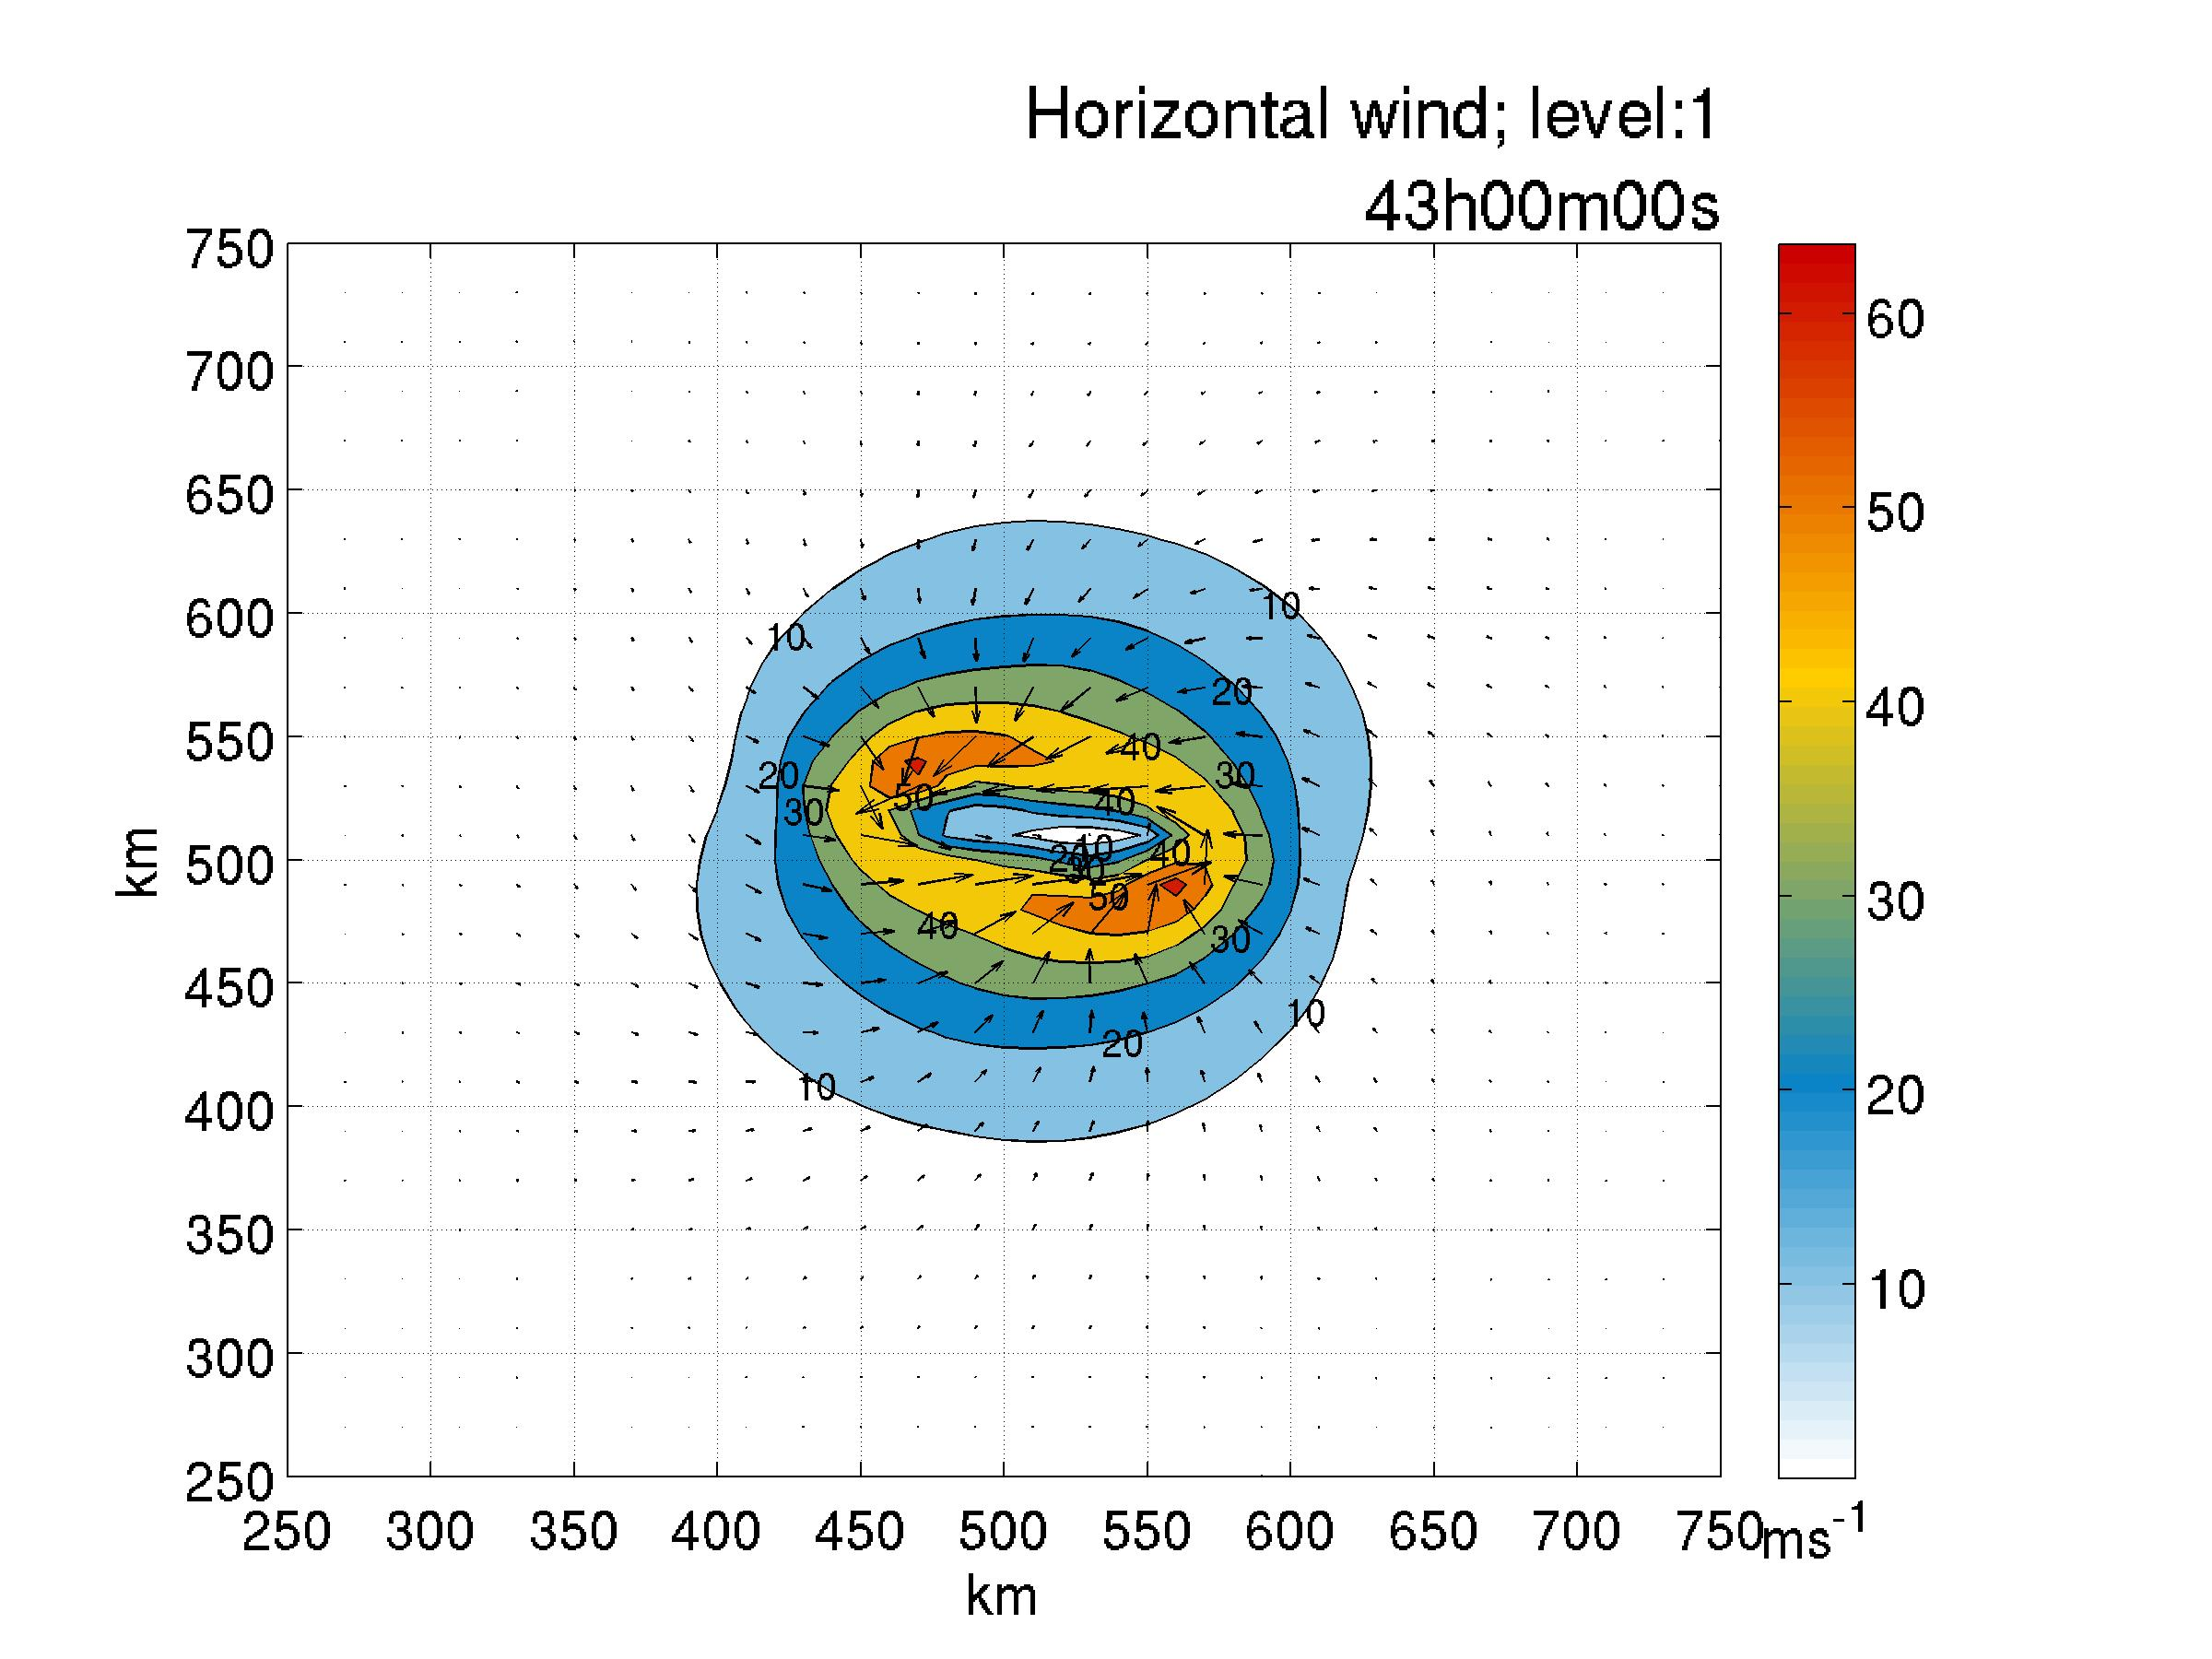
\includegraphics[width=\linewidth]{{./chapters/figures_results/ctrl_fields/VectorWind_z.x26-x76.y26-y76.ilev01.430000}.jpg}
\end{center}
\caption{Поле горизонтальной скорости ветра (фокус $500\times 500\km$). Эксперимент CTRL. 43 час модельного времени.}
\label{fig:ctrl_split_hwind}
\end{wrapfigure} 

В этом контексте был проведен дополнительный эксперимент (не показано) на расчетной области большего размера и с меньшими ограниченими на допустимые скорости ветра. При этом центральное циклоническое возмущение сначала разделялось на две части, которые двигались в противоположные стороны и, в свою очередь, разделялись на две части, каждая из которых также делилась на две части, и так далее. При этом каждый раз вихри меньшего размера делили общую КЭ поровну и продолжали интенсифицироваться. 

Можно предположить, что разделение вихря --- это реализация прямого каскада энергии по спектру. Энергия 'накачивается' на узком диапазоне волновых чисел, соответствующих изолированному возмущению, а затем сбрасывается в более мелкие масштабы через разделение вихря. Для проверки этой гипотезы был построен спектр.....................

%\subsection{Энергетическая диагностика}
%Перейдем к анализу динамики возмущения с точки зрения энергетики атмосферы. На рис. \ref{fig:ctrlene} представлена эволюция интегральной кинетической энергии. В данном случае величина общей кинетической энергии и кинетической энергии возмущений, очевидно, совпадает, так как в модельной области развивается только рассматриваемый циклон. Сначала ход кинетической энергии испытывает колебание, связанное с испусканием инерционно-гравитационных волн. Затем она непрерывно растет до значений порядка $10\Jpm$, что согласуется с результатами идеализированного моделирования других авторов (например, \citep{YanaseNiino2007}). При этом скорость роста энергии даже больше, чем по экспоненциальной зависимости. 
%
%\begin{wrapfigure}{R}{0.5\textwidth}
%\begin{center}
%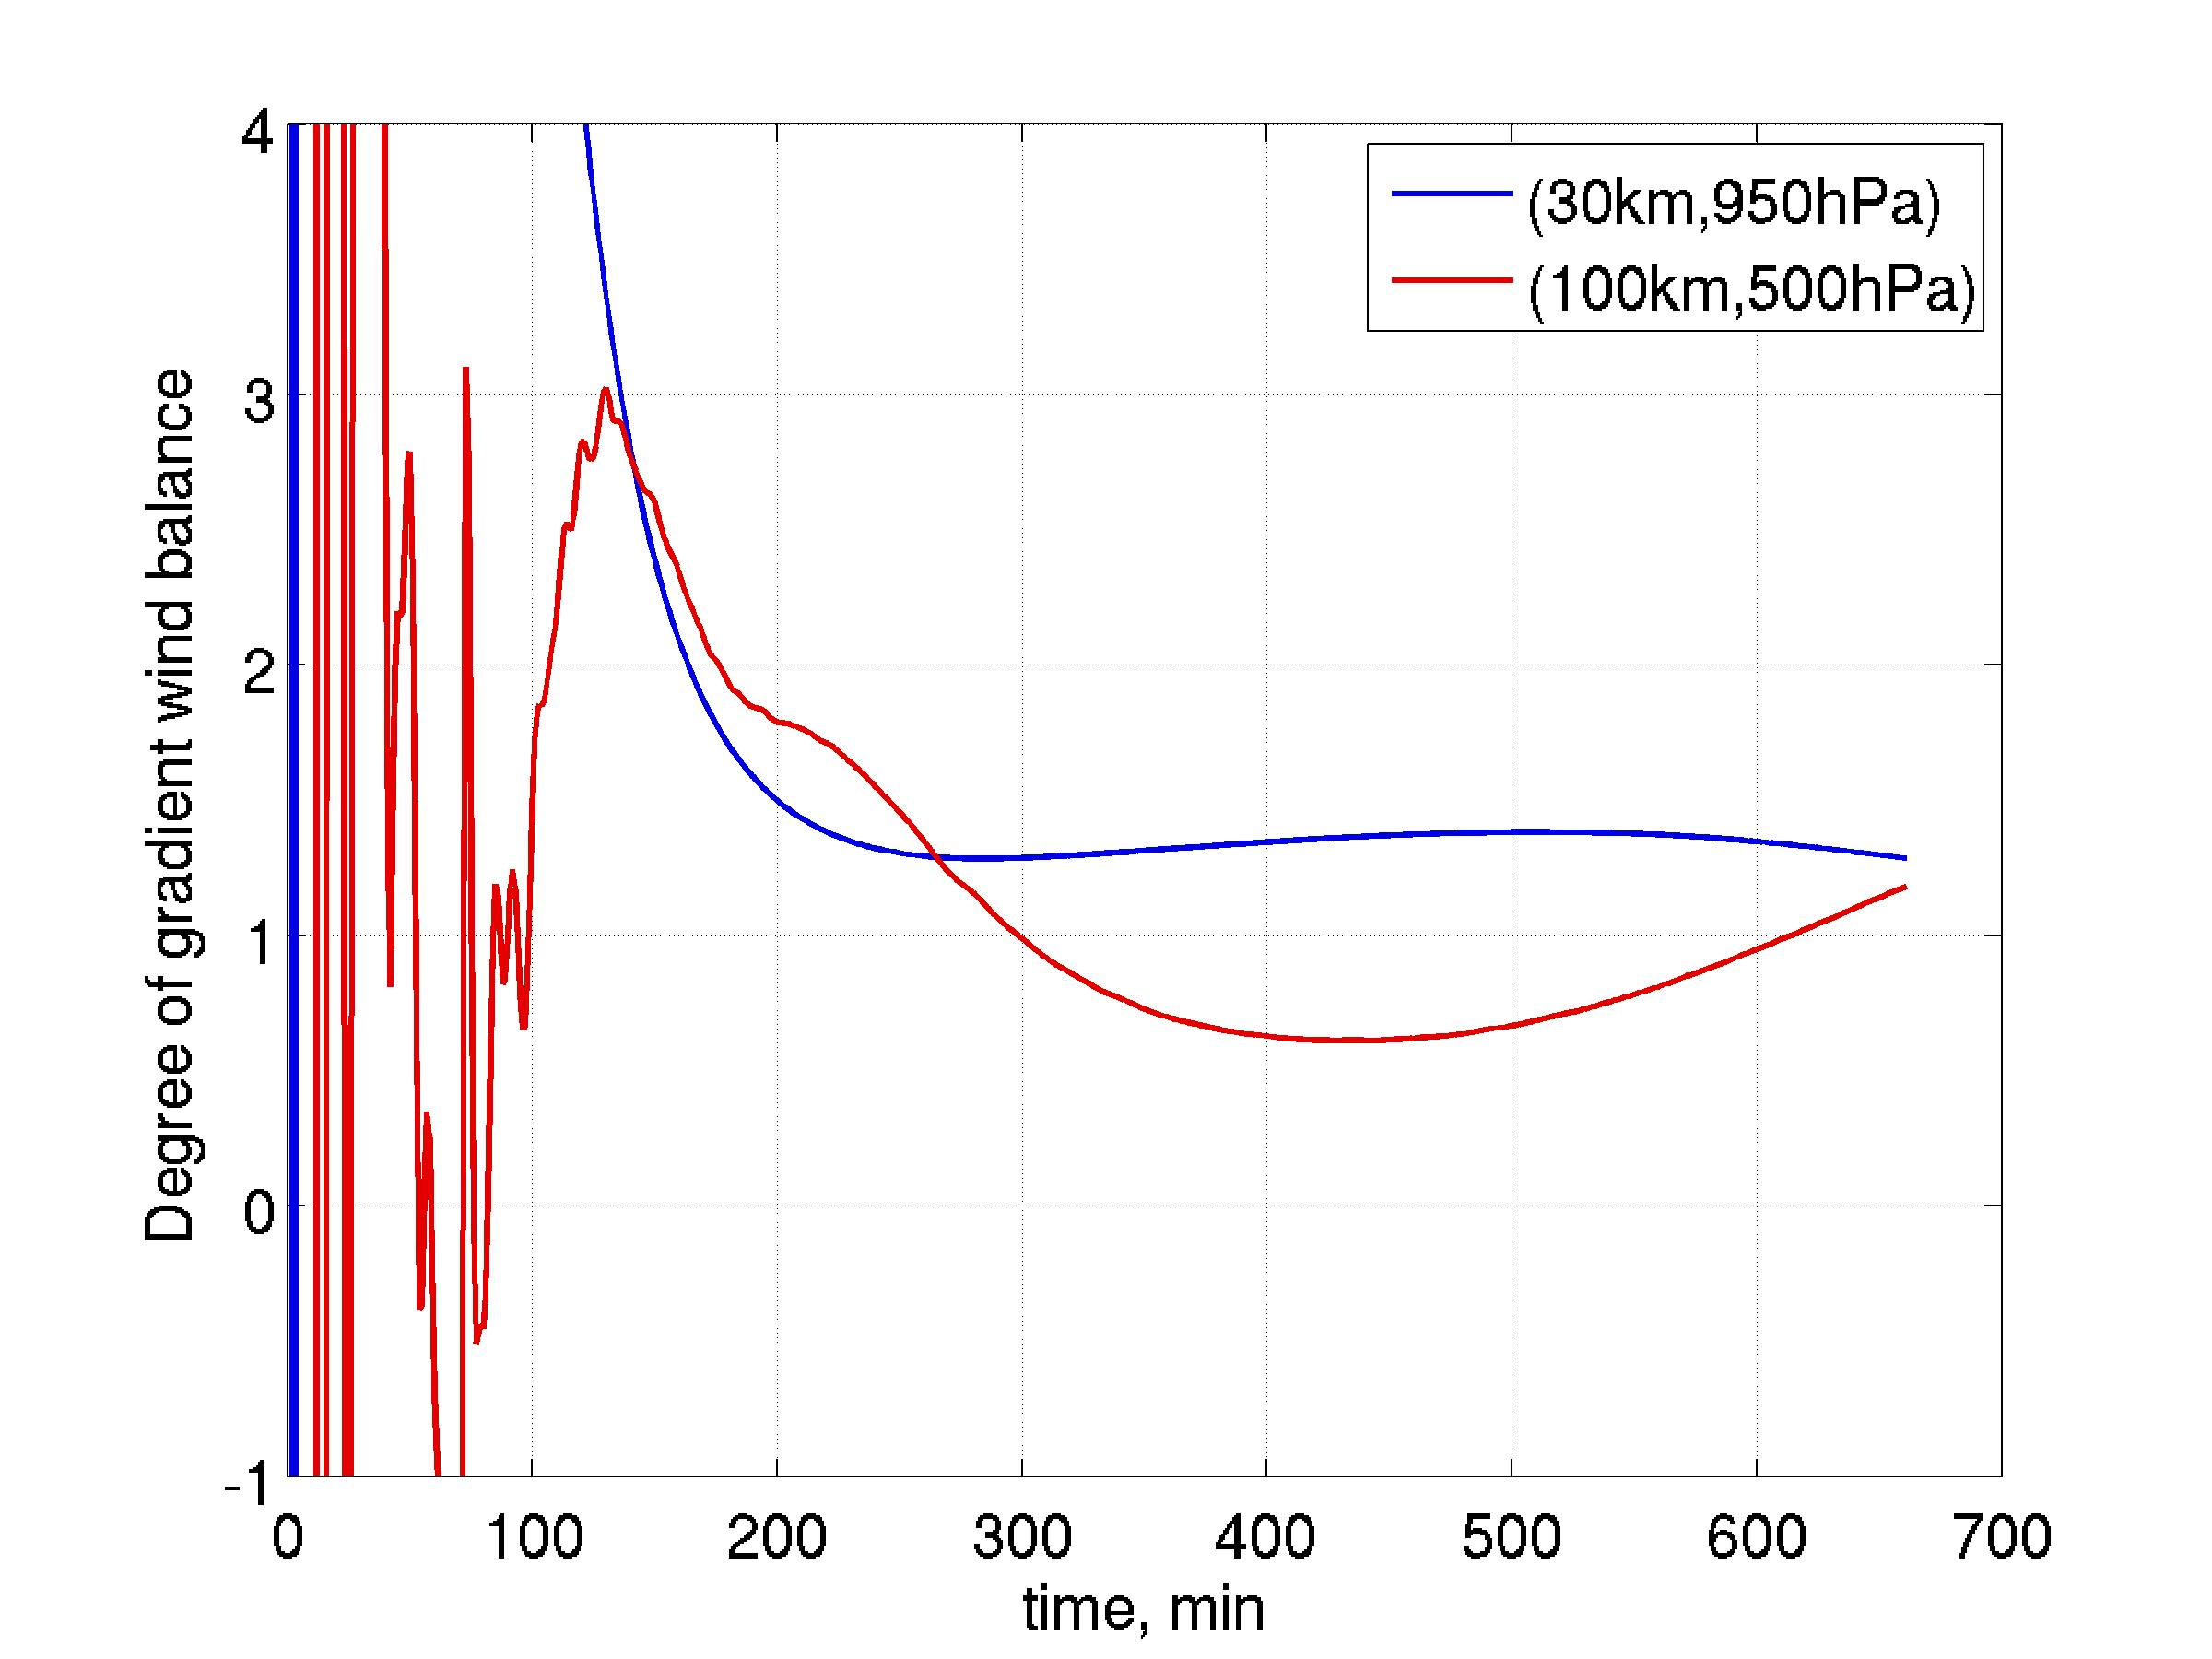
\includegraphics[width=\linewidth]{{./chapters/figures_results/ctrl_grwindbal2p}.jpg}
%\end{center}
%\caption{Вертикальный разрез вертикальной скорости $w$. Эксперимент CTRL. ??? час модельного времени.}
%\label{fig:ctrl_ene}
%\end{wrapfigure} 
%
%За счет чего развивается рассматриваемый мезоциклон? Для ответа на этот вопрос приводится бюджет кинетической энергии (рис. \ref{fig:ctrl_ene}), рассчитанный согласно ур. \ref{eq:dKdt}. Видно, что наиболее важными слагаемыми бюджета энергии являются слагаемое $C(A,K)$ перехода доступной потенциальной энергии в кинетическую и слагаемое диссипации кинетической энергии. Оба слагаемых растут по абсолютным значениям по мере роста энергии движения в вихре. 
%
%Интегральная величина $C(A,K)$ физически представляет собой поток силы плавучести $w\frac{\theta'}{\theta_s}$, суммированный по всей области. Его распределение в циклоне показано на рис. \ref{fig:ctrl_buoy_rz}. Можно заметить, что области экстремумов величины $w\frac{\theta'}{\theta_s}$ совпадают с областями наибольших и наименьших значений вертикальной скорости. Иными словами, конвертация ДПЭ в КЭ в моделируемом мезоциклоне наиболее интенсивна на радиусе максимальной скорости.
%Слагаемое $C(A,K)$, определяя тенденцию кинетической энергии, связывает ее с изменением доступной потенциальной энергии. При этом в бюджете последней это слагаемое имеет сравнительно малую долю (рис. \ref{}). Доступная потенциальная энергия в свою очередь генерируется за счет  слагаемого $H_{surf}$, связанного с потоками тепла на нижней границе области (\ref{sec:expsetup:hsurf}).
%
%\section{'Влажный' эксперимент: эффекты конденсации} 
%
%\begin{wrapfigure}{R}{0.5\textwidth}
%\begin{center}
%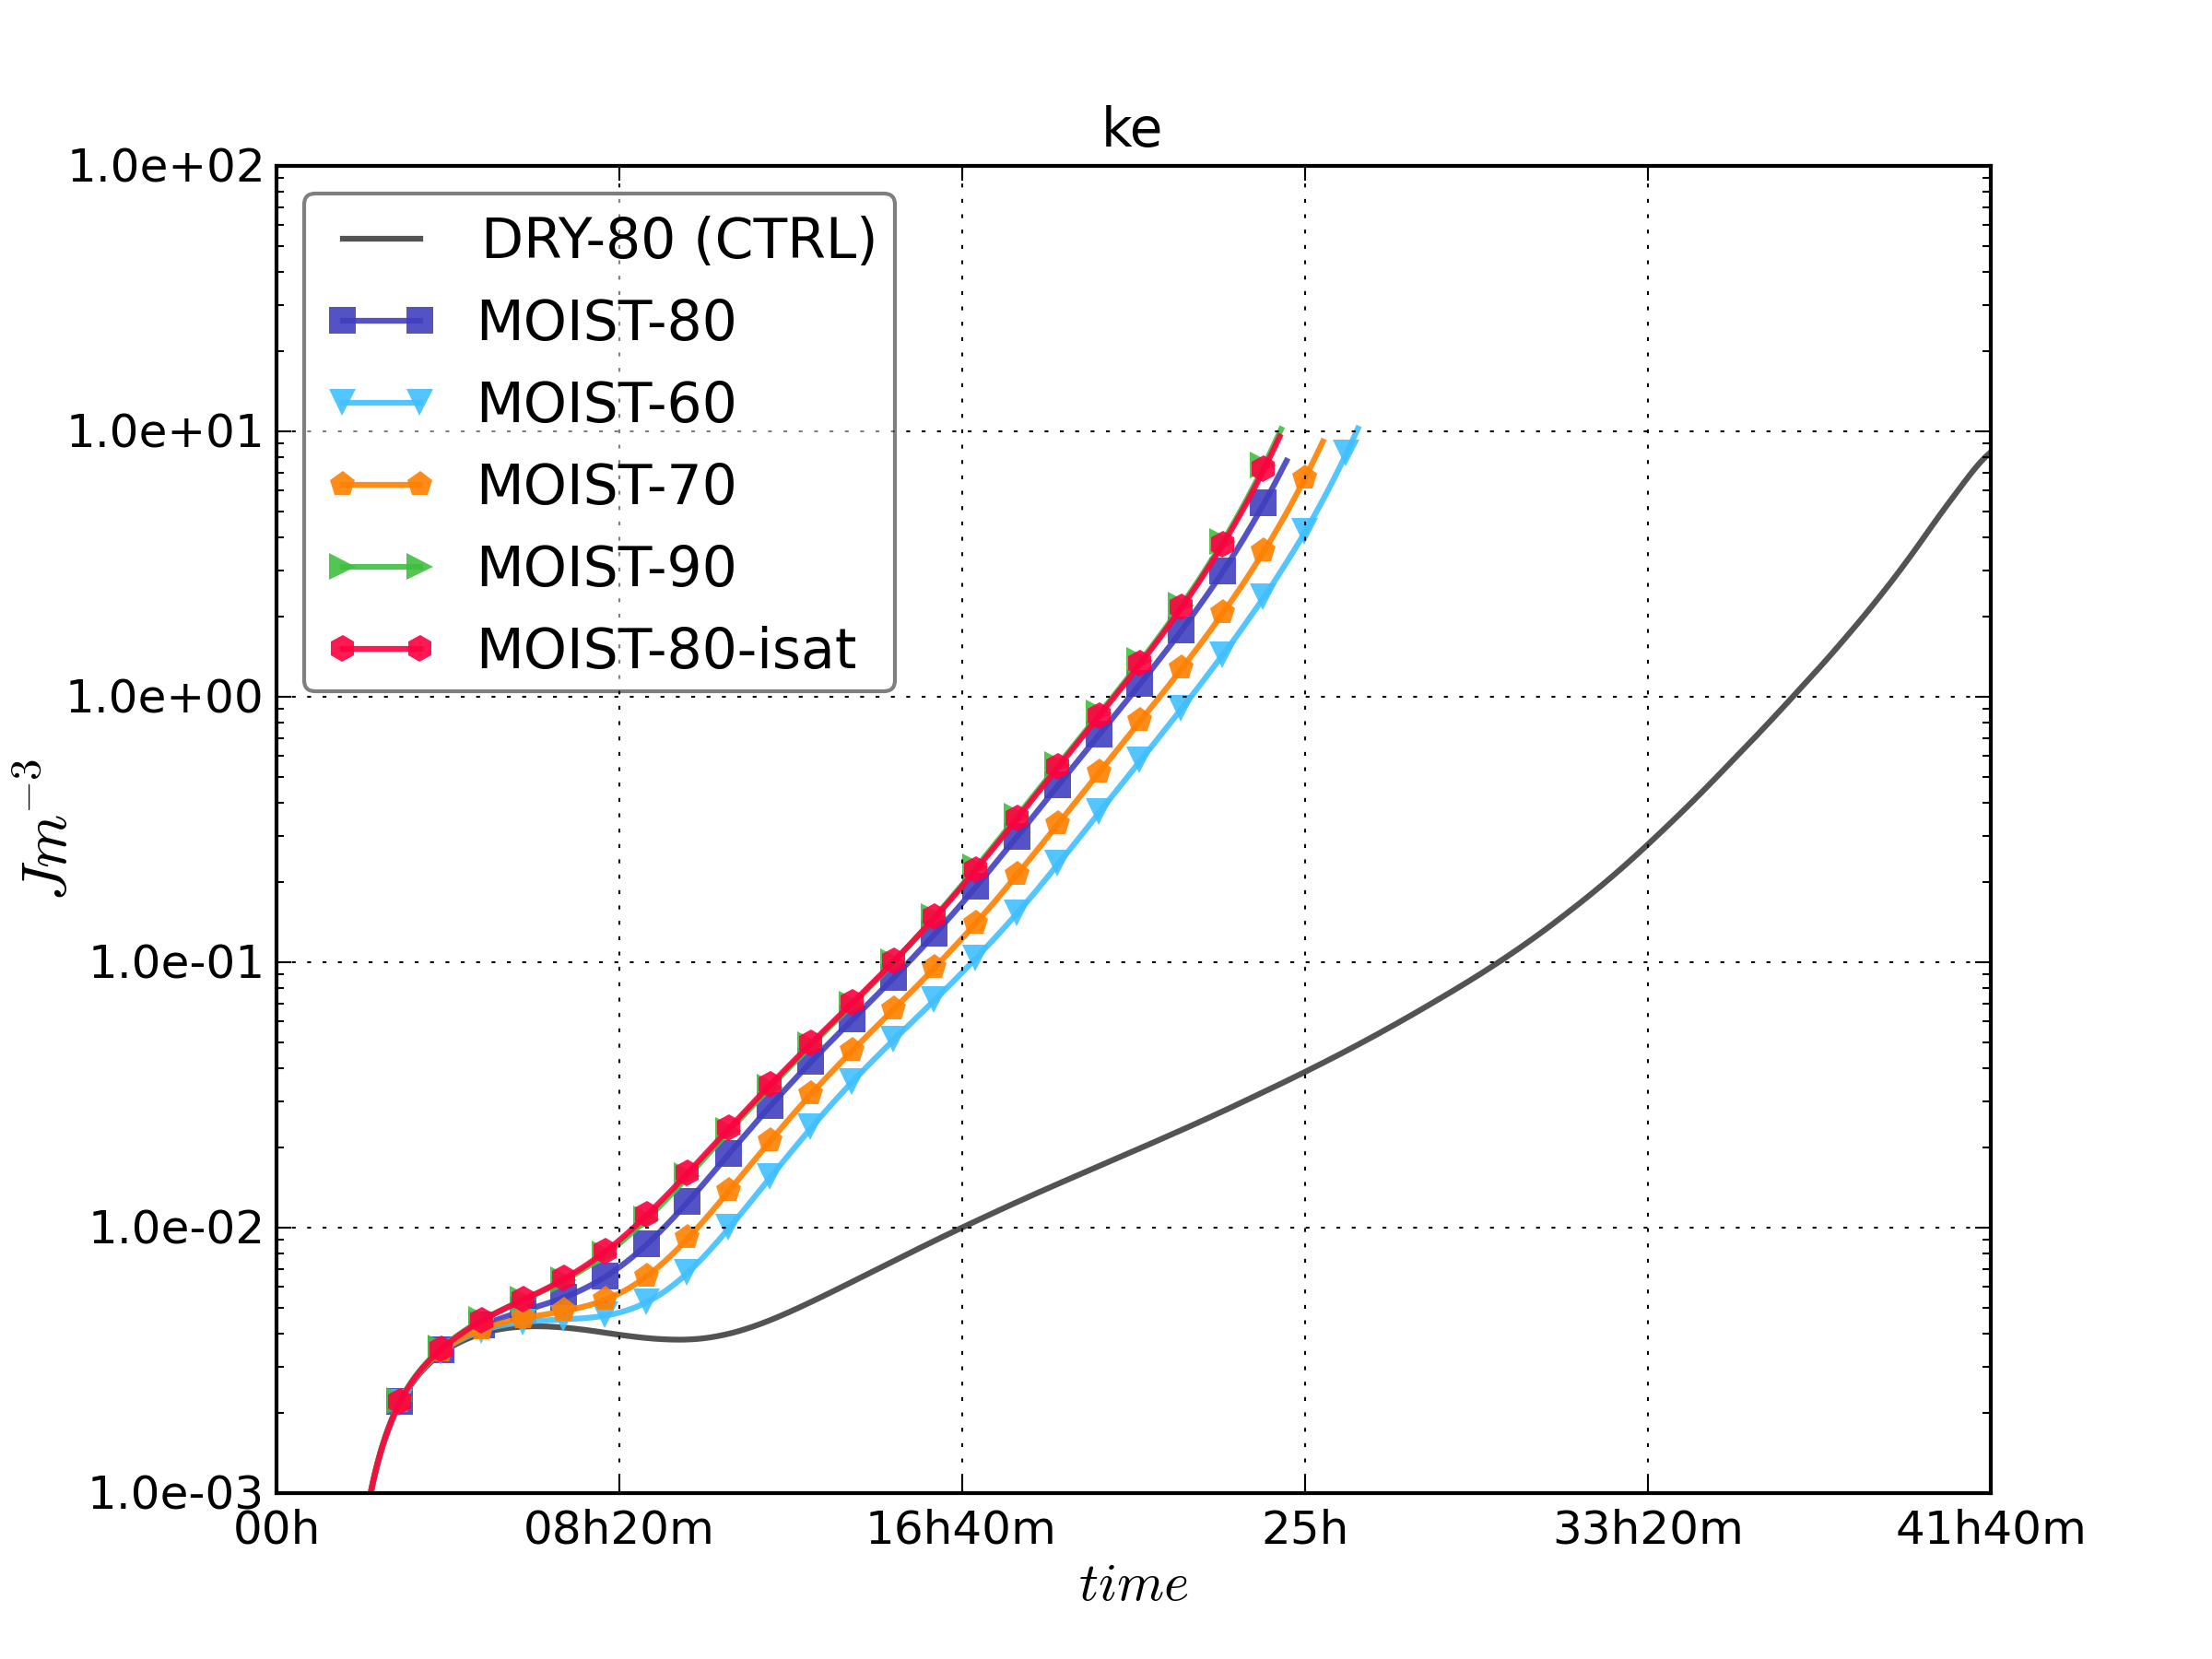
\includegraphics[width=\linewidth]{{./chapters/figures_results/ke.00h-41h38m.DRYvsMOIST}.png}
%\end{center}
%\caption{Эволюция кинетической энергии в экспериментах MOIST по сравнению с контрольным (здесь и далее черная кривая).}
%\label{fig:moist_ke}
%\end{wrapfigure} 
%
%Напомним, что описанный выше контрольный эксперимент является 'сухим': процессы конденсации были отключены, несмотря на то, что относительная влажность в центре области довольно скоро начала превышать $100\%$. Для того, чтобы оценить влияние конденсации в атмосфере как дополнительного источника тепла, проанализируем серию 'влажных' экспериментов (MOIST). На рис. \ref{fig:moist_ke} представлено изменение кинетической энергии со временем экспериментах MOIST (цветные кривые) по сравнению с контрольным экспериментом (DRY, черная кривая). Эксперименты с конденсацией характеризуются большей скоростью роста энергии и, соответственно, меньшим временем устойчивости эксперимента: вихрь развивается до предельных скоростей ветра ровно за сутки. 
%
%Аналогичное соотношение между сухим и влажным экспериментом дает сравнение роста аномалии приземного давления ($SLP_{anom}$), который показан на рис. \ref{fig:moist_slp}. Максимальное падение давления в центре в эксперименте MOIST-80 составляет $-32.6\hpa$, в то время как в контрольном эксперименте (черная кривая) минимум давления в центре вихря достигает $19.8\hpa$.
%
%\begin{wrapfigure}{L}{0.5\textwidth}
%\begin{center}
%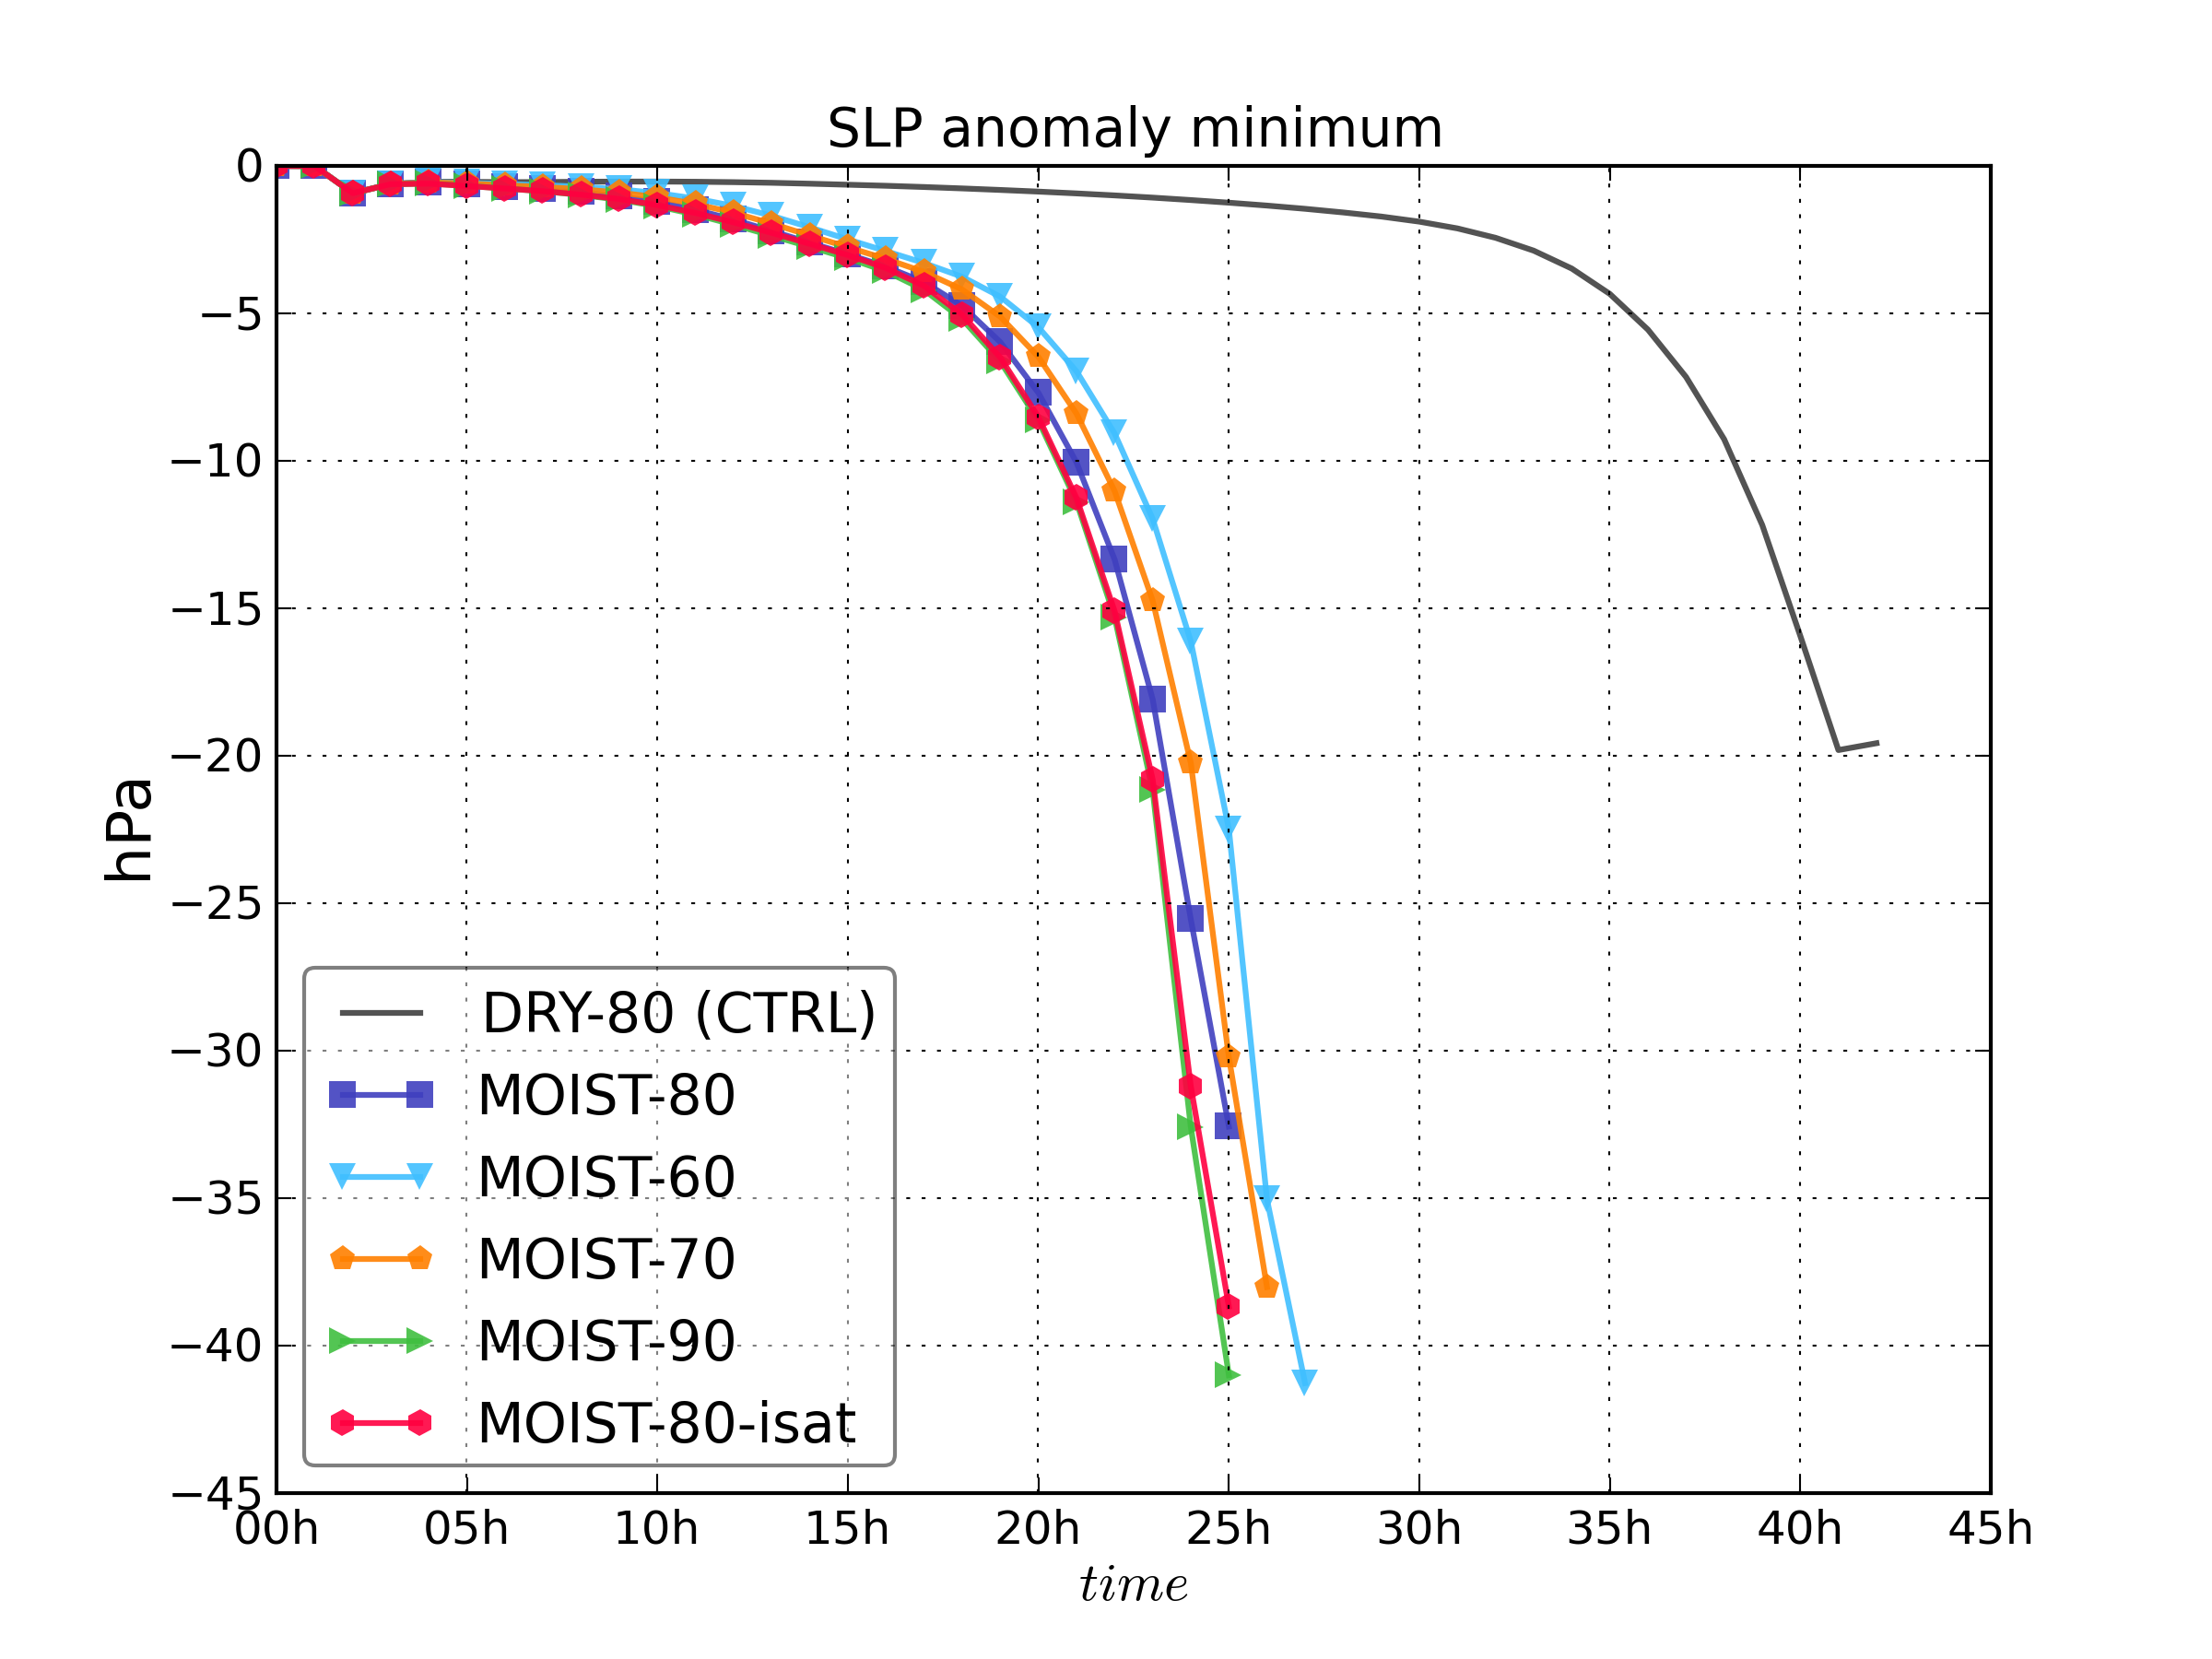
\includegraphics[width=\linewidth]{{./chapters/figures_results/slp_min.00h-42h.DRYvsMOIST}.png}
%\end{center}
%\caption{Эволюция аномалии приземного давления в экспериментах MOIST по сравнению с контрольным.}
%\label{fig:moist_slp}
%\end{wrapfigure} 
%
%Представленные графики показывают зависимость интенсивности вихря от начального содержания влаги в атмосфере: чем больше относительная влажность воздуха задана в начальный момент, тем интенсивнее происходит развитие вихря: так, в  25 час модельного времени аномалия приземного давления составляет от $-22\hpa$ до $-41\hpa$ для экспериментов от MOIST-60 до MOIST-90 соответственно.
%
%Проведенные эксперименты позволяют оценить чувствительность динамики вихря к содержанию влаги в атмосфере. Сначала определим показатель интенсивности вихря как единый количественный критерий для всех экспериментов, разделив минимум аномалии приземного давления в расчетной области на время достижения этого минимума. Это позволит более корректно сравнивать эксперименты, в которых циклон развивался до одинаковой силы, но за разный период времени. Иначе говоря, в качестве показателя интенсивности вихря берется средняя барическая тенденция:
%\begin{equation} \label{eq:intensity}
%I = \frac{SLP_{anom}}{\tau},
%\end{equation}
%где $SLP_{anom}$ --- аномалия приземного давления (\ref{eq:slpanom}), $\tau$ --- продолжительность экспепримента ($\tau_{max}=72$ ч.). Разность между интенсивностью вихря $I$ в контрольном эксперименте и интенсивностью в оценочном эксперименте, отнесенная к разности значения какого-либо параметра $P$ (в данном случае начальной влажности воздуха) дает показатель чувствительности:
%\begin{equation}
%S_{slp}=\frac{\delta I}{\delta P}.
%\end{equation}
%Используя этот показатель, результаты серии оценочных экспериментов MOIST можно представить в количественном выражении (табл. \ref{}, аналогично \citep{LindersEtAl2011}).
%
%\begin{table}
%\end{table}
%
%Кривая MOIST-80-isat относится к эксперименту, в котором фазовые переходы воды зависят от формулы давления насыщения водяного пара надо льдом, а относительная влажность воздуха равна контрольной. На рис. \ref{fig:moist_ke} и \ref{fig:moist_slp} эта кривая почти совпадает с кривой MOIST-90, т.е. использование в модели формулы Магнуса (закона Клаузиуса-Клапейрона) для давления насыщения водяного пара надо льдом по сравнению с таковой для давления насыщения над водой равносильно ошибке в задании начальной относительной влажности, равной около $10\%$. Однако к кардинальным отличиям в динамике вихря использование той или иной формулы не ведет.
%
%\subsection{Энергетическая диагностика}
%Различия в темпах роста мезоциклона в рассматриваемых экспериментах можно рассмотреть с точки зрения генерации кинетической энергии. Как и в контрольном эксперименте, основной вклад в бюджет кинетической энергии вносит слагаемое $C(A,K)$, которое по значениям также пропорционально количеству влаги в атмосфере. На рис. \ref{fig:moist_dkdt}, где представлены компоненты энергии для выбранных случаев, четко прослеживается отличие контрольного эксперимента от серии MOIST, причем это наблюдается для всех величин ввиду их нелинейности.
%
%\begin{wrapfigure}{R}{0.5\textwidth}
%\begin{center}
%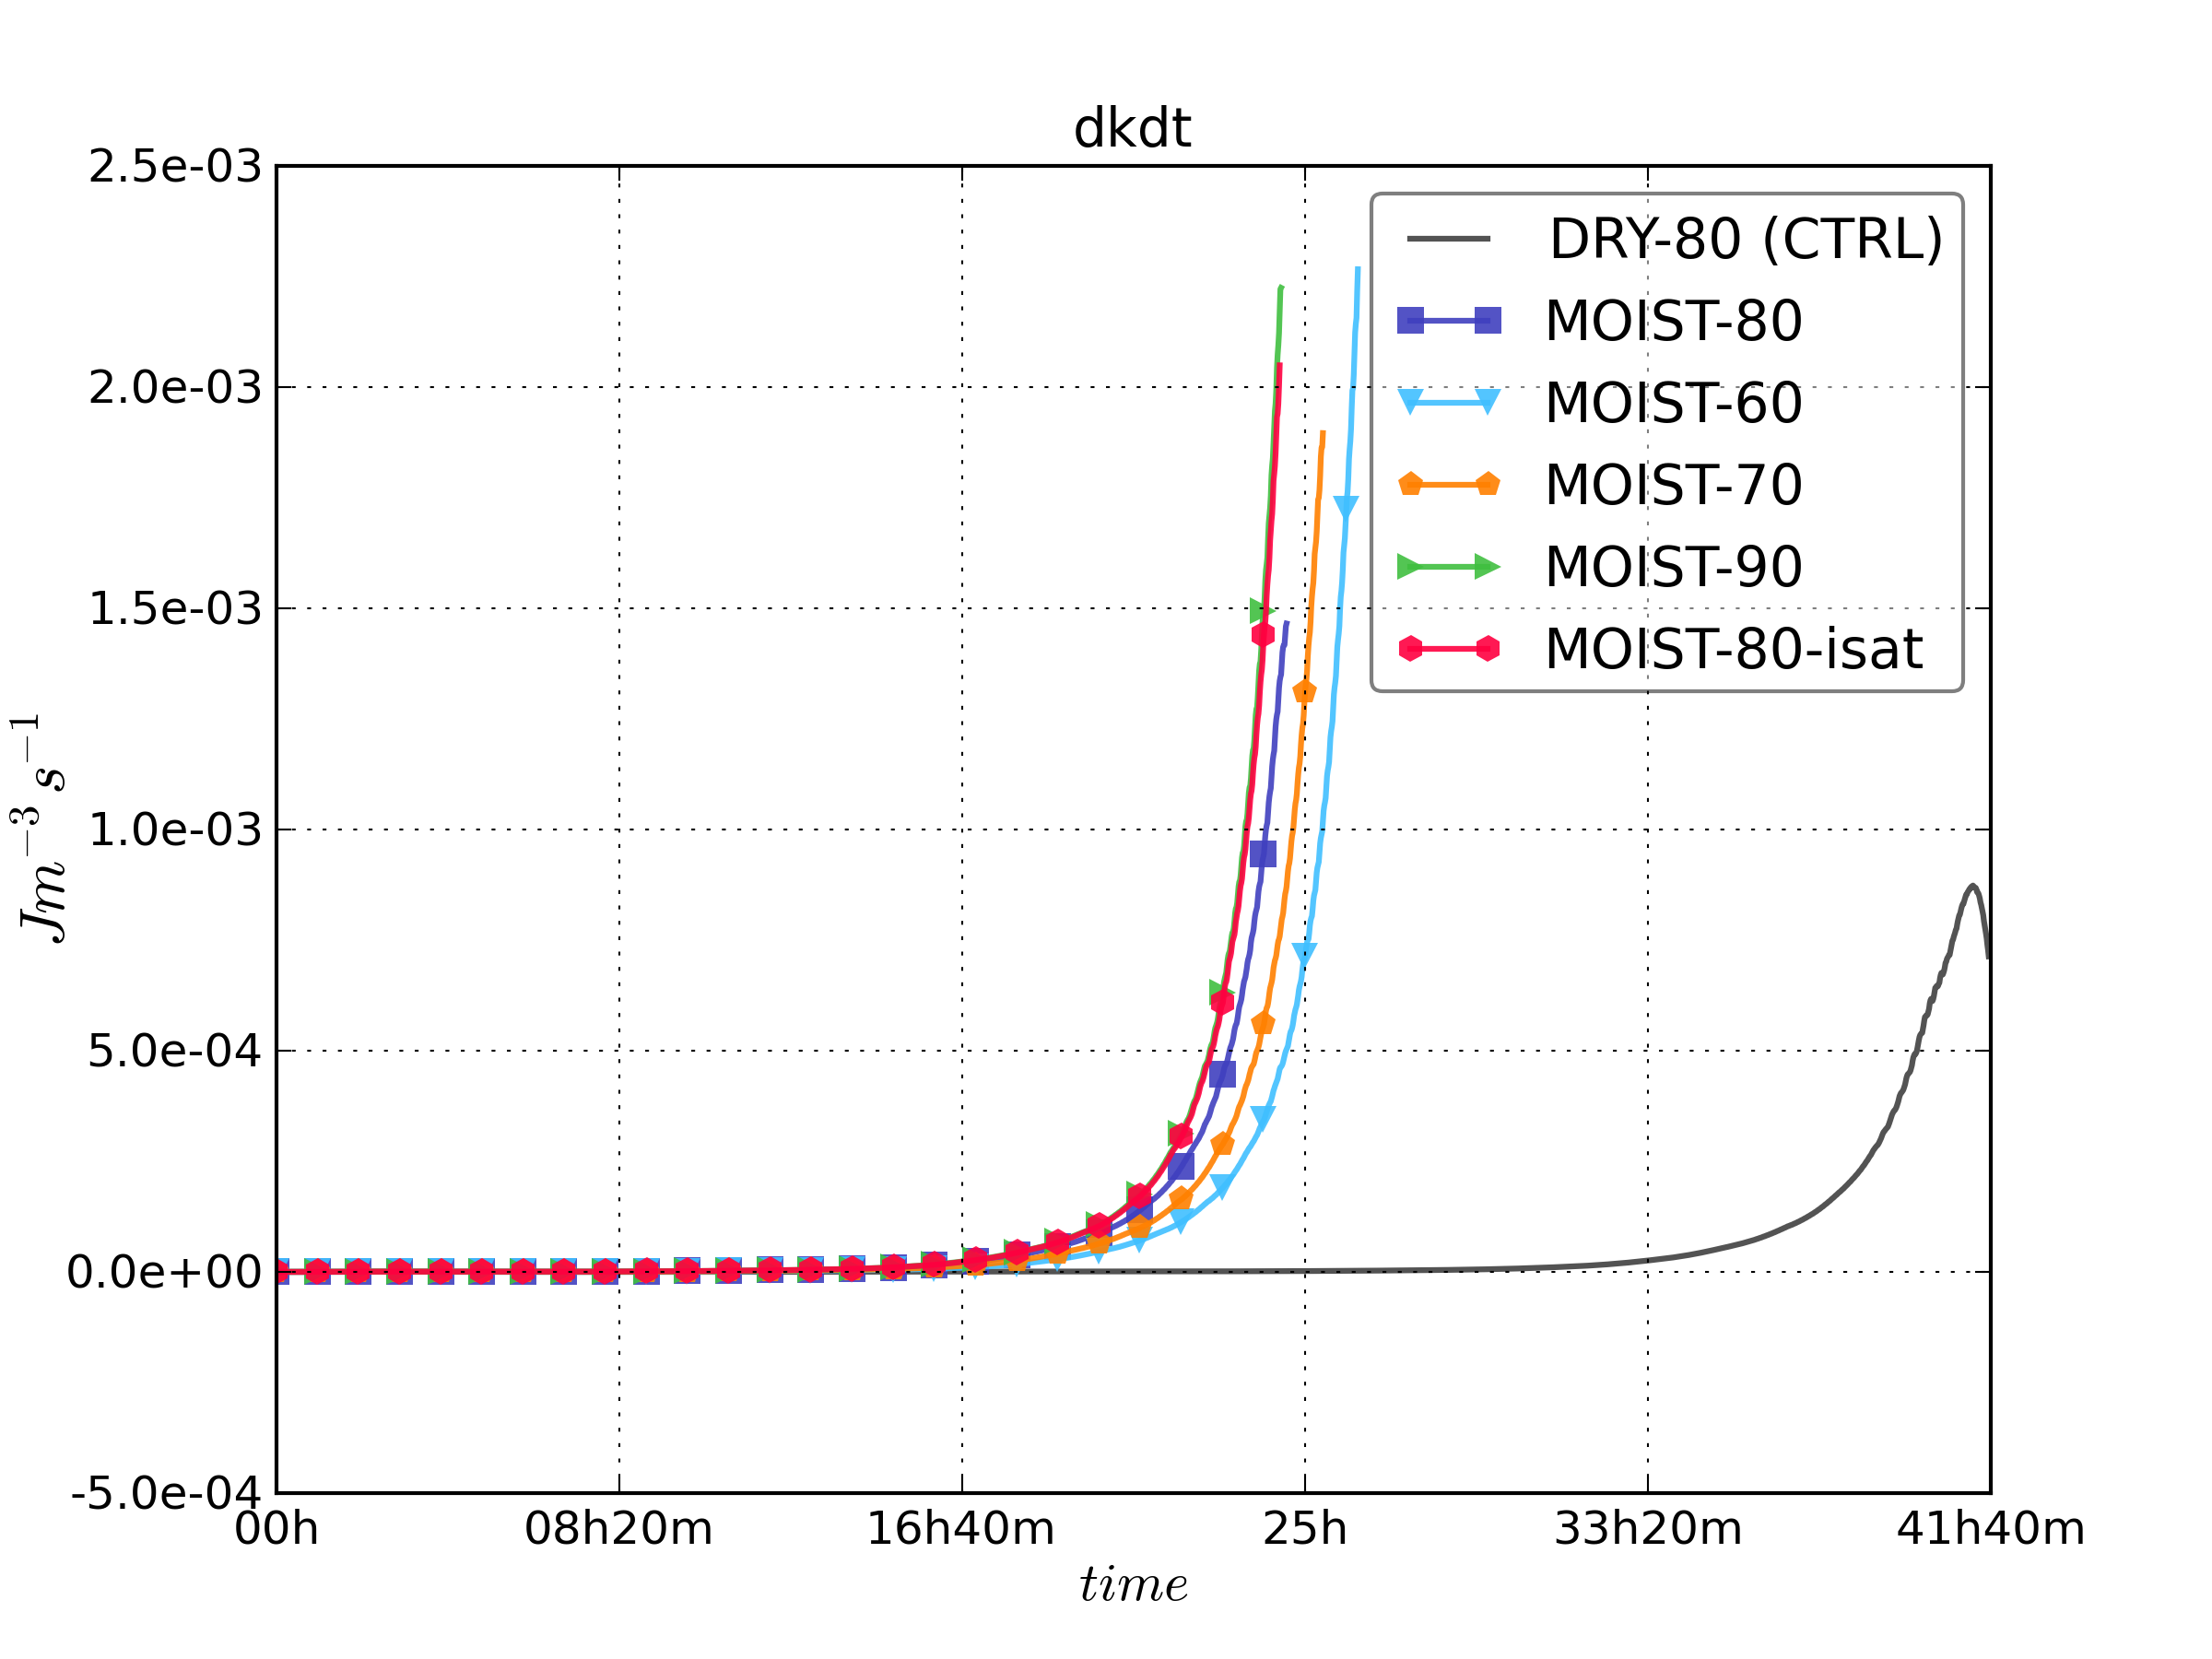
\includegraphics[width=\linewidth]{{./chapters/figures_results/dkdt.00h-41h38m.DRYvsMOIST}.png}
%\end{center}
%\caption{Изменение скорости роста кинетической энергии в экспериментах MOIST по сравнению с контрольным.}
%\label{fig:moist_dkdt}
%\end{wrapfigure} 
%
%Дополнительным источником энергии для роста циклона, очевидно, являются неадиабатические процессы, т.е. выделение скрытого тепла конденсации (ур. \ref{eq:progn4}, второе слагаемое в правой части). В ходе анализа экспериментов недиабатический приток тепла был рассчитан по остаточному методу \citep{Muench1965,MooreMontgomery2005}:
%\begin{equation}
%Q=\left[\pderiv{\theta}{t}+\vec{v}\cdot\nabla_h\theta+\omega\pderiv{\theta}{p}\right]c_p\left(\frac{p}{p_{00}}\right)^{R_d/c_p},
%\end{equation}
%где $\pderiv{}{t}+\vec{v}\cdot\nabla_h+\omega\pderiv{}{p}$ --- полная производная в $p$-системе координат. Расчет проводился по данным, интерполированным на изобарические поверхности. Далее для удобства величину $Q$ разделим на $c_p$ и умножим на $86400$, получив размерность $\K~\text{день}^{-1}$. На рис. \ref{} представлено сравнение недиабатического притока тепла для выбранных экспериментов, из которого понятно, что в каждом эксперименте рост этой величины начинается в разное время для разных экспериментов, так как состояние насыщения достигается тем быстрее, чем больше относительное влагосодержание воздуха при инициализации. Для контрольного эксперимента же недиабатический приток тепла остается на уровне ??? $\K~\text{день}^{-1}$ (вклад потоков тепла с поверхности).
%
%\subsection{Структура и эволюция вихря}
%Вклад энергии от фазовых переходов воды отражается на строении моделируемого мезоциклона. Для этого на рис. \ref{} приведены радиальные разрезы основных метеорологических полей, полученные в эксперименте MOIST-80, за 18 час модельного времени, когда скорость ветра в мезоциклоне сопоставима с таковой  в контрольном эксперименте за 36 час.
%
%В основном, различие между контрольным экспериментом (DRY-80) и MOIST-80 проявляется в распределении влагосодержания воздуха: вблизи центра вихря закономерно происходит уменьшение содержания водяного пара в процессе конденсации. Распределение конденсации в циклоне находится в соответствии с полем относительной влажности (рис. \ref{}), и максимум приходится на область конвективных движений (рис. \ref{}) на расстоянии $30$--$40\km$ от центра и на высоте $2000\m$. Из представленных разрезов также ясно, что слабая конденсация происходит и на периферии вихря вследствие турбулентного потока влаги с поверхности.
%
%\section{Серия с разной устойчивостью атмосферы}
%\subsection{Влияние устойчивости атмосферы на интенсивность вихря}
%К важным факторам, оказывающим влияние на развитие атмосферных неоднородностей, относится стратификация атмосферы. Размеры возмущений и статификацию объединяет в себе радиус деформации Россби ($R=\frac{Nf}{L}$). Это число показывает, что вертикальный масштаб циклона, возникшего в результате нагрева, обратно пропорционально статической устойчивости и прямо пропорционально абсолютной завихренности и горизонтальному масштабу объекта.
%
%\begin{figure}[h]
%	\centering
%	\begin{subfigure}{0.45\textwidth}
%		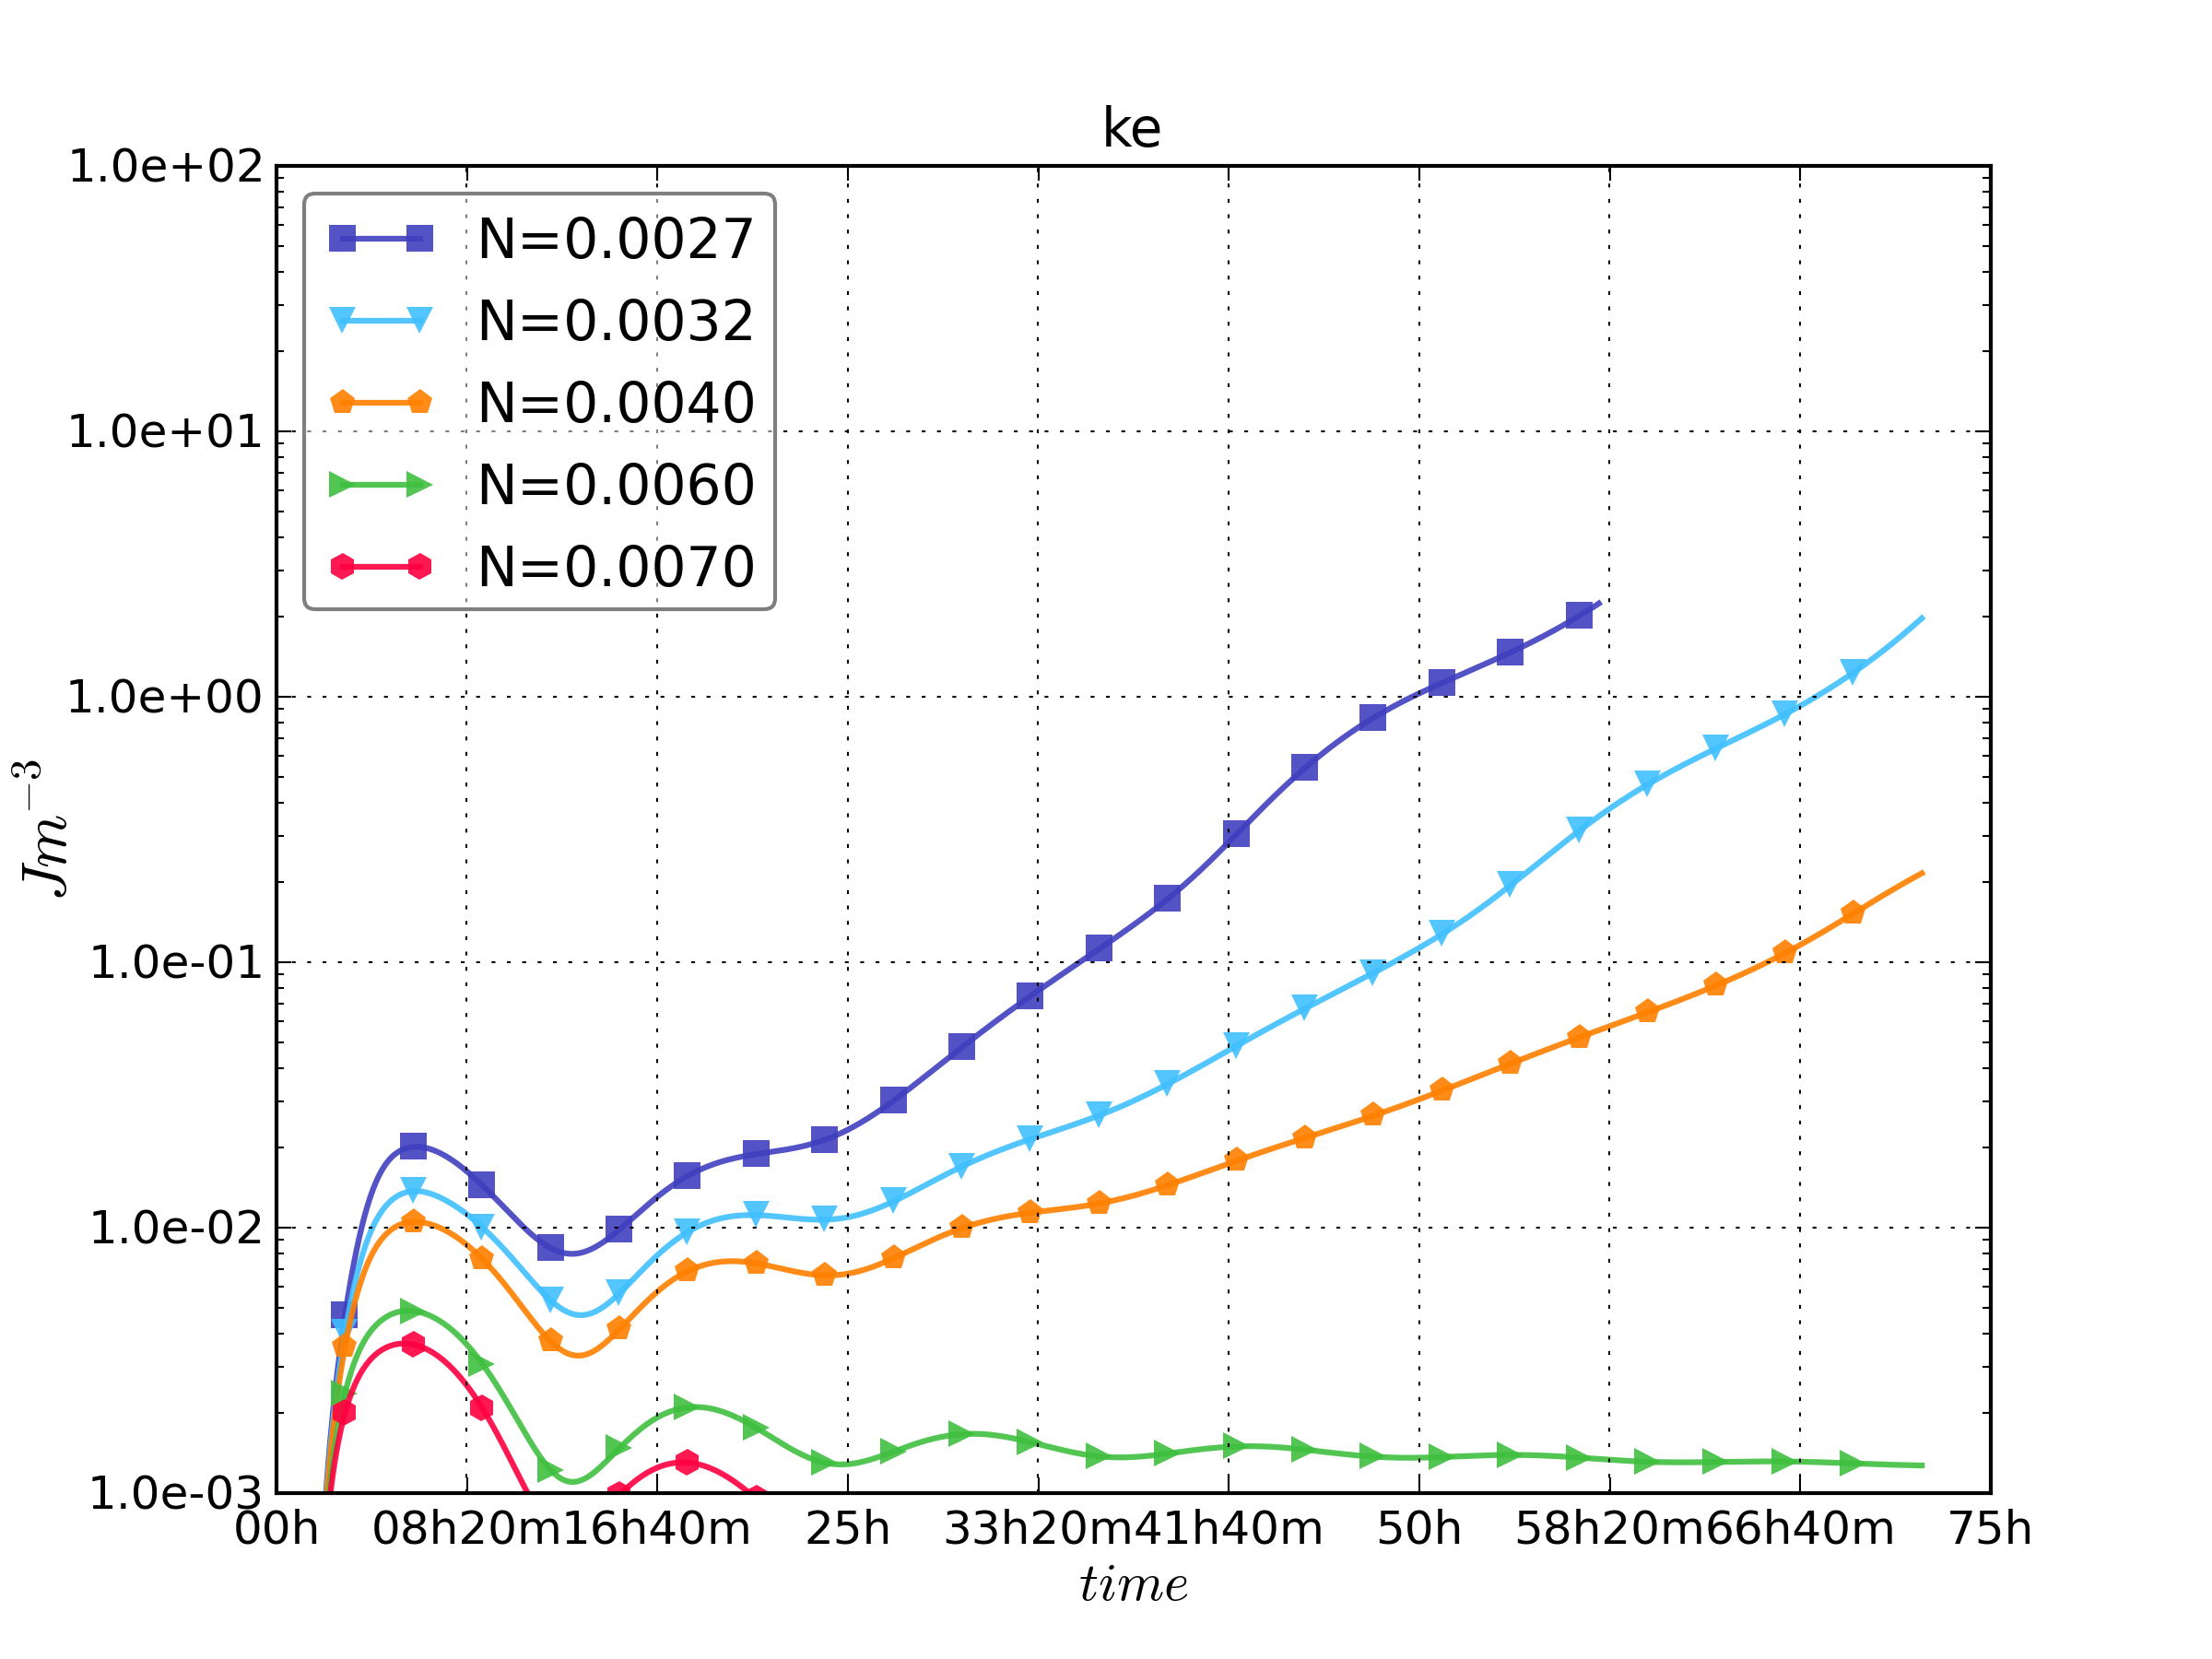
\includegraphics[width=\linewidth]{{./chapters/figures_results/ke.00h-72h.lowN}.png}
%		\caption{ }
%        \label{fig:lowN_ke}
%	\end{subfigure}
%	\hfill
%	\begin{subfigure}{0.45\textwidth}
%		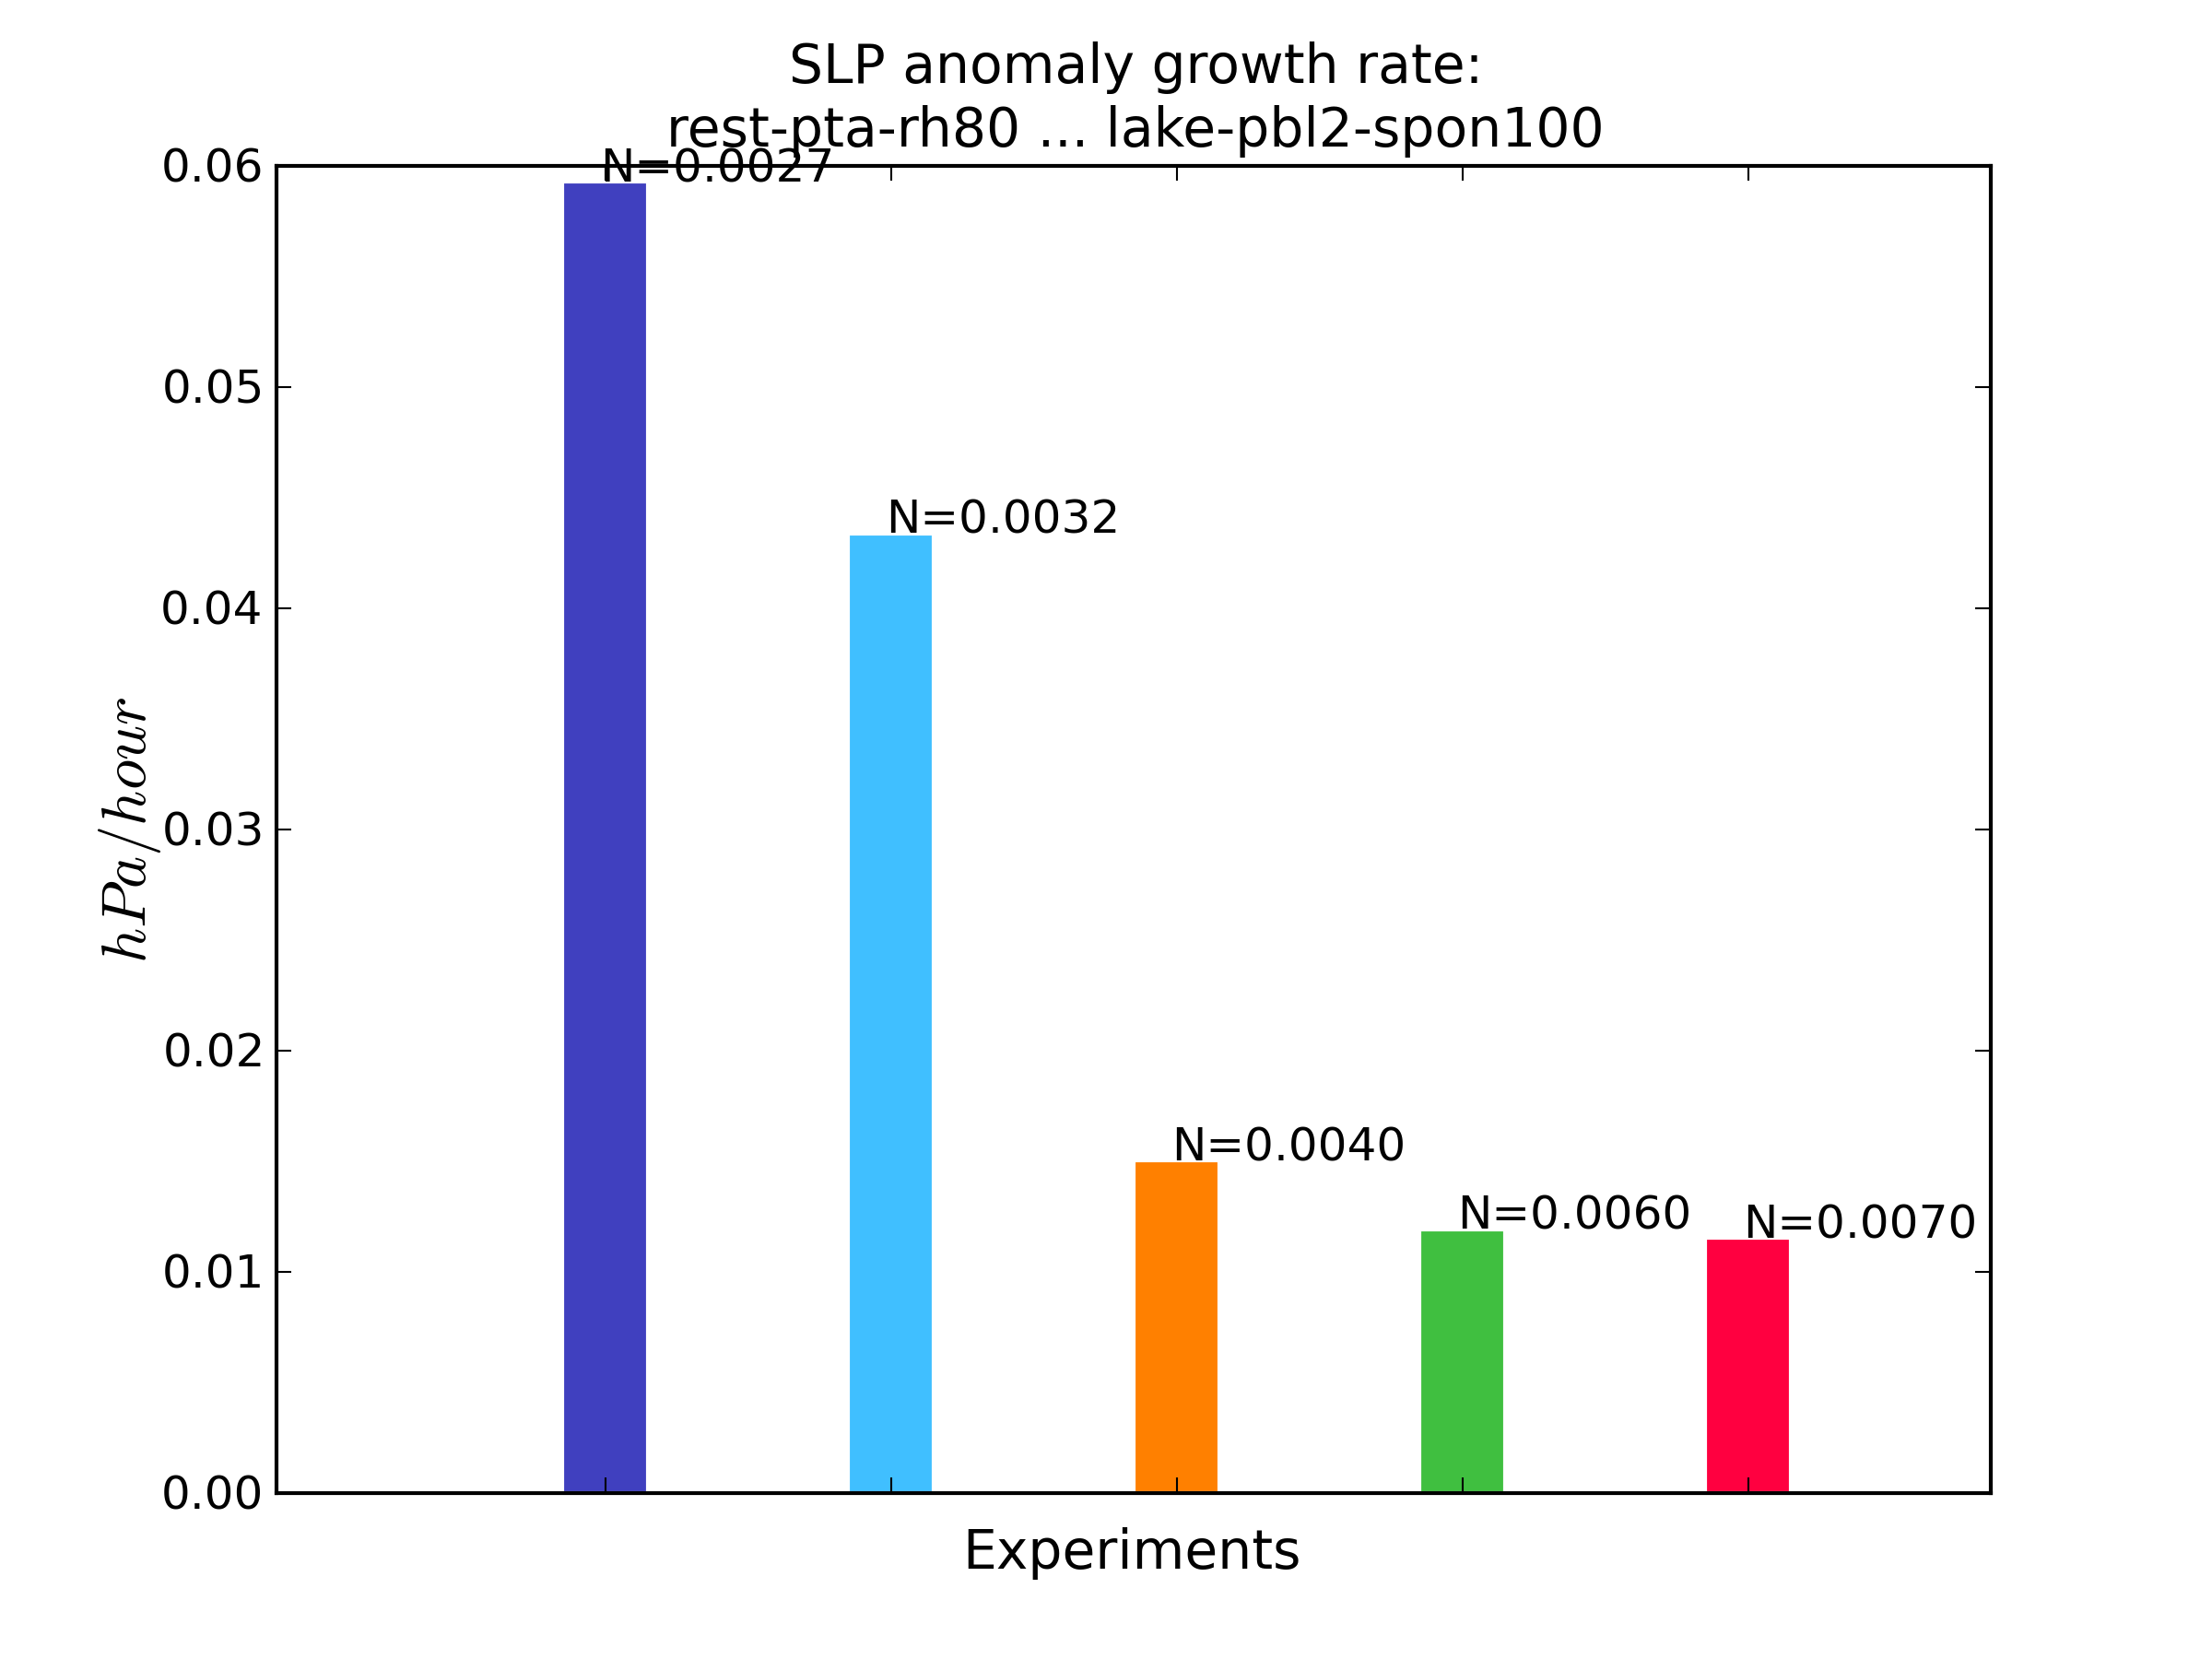
\includegraphics[width=\linewidth]{{./chapters/figures_results/slp_min_rate.00h-73h.lowN}.png}
%		\caption{ }
%		\label{fig:lowN_slp_rate}
%	\end{subfigure}
%        \caption{Эксперименты с пониженной устойчивостью фоновой атмосферы: изменение во времени кинетической энергии (слева) и чувствительность вихря к $N$ (справа).}
%\end{figure}
%
%Чувствительность развивающегося мезоциклона к устойчивости атмосферы была оценена с помощью серии экспериментов, в которых при неизменной температуре нижнего слоя менялась температура остальной толщи атмосферы, создавая вертикальный градиент потенциальной температуры от $0.2\Kpkm$ до $8\Kpkm$. То есть диапазон условий варьировался от статически нейтральной стратификации до устойчивой стратификации, характерной для арктических воздушных масс и в среднем наблюдающейся при генерации мезоциклонов \citep{ForbesLottes1985}. Частота Брента-Вяйсяля $N$ как показатель устойчивости атмосферы имел для фоновой стратификации значения $0.0027$--$0.0160\pers$ соответственно.
%
%\begin{figure}[h]
%	\centering
%	\begin{subfigure}{0.45\textwidth}
%		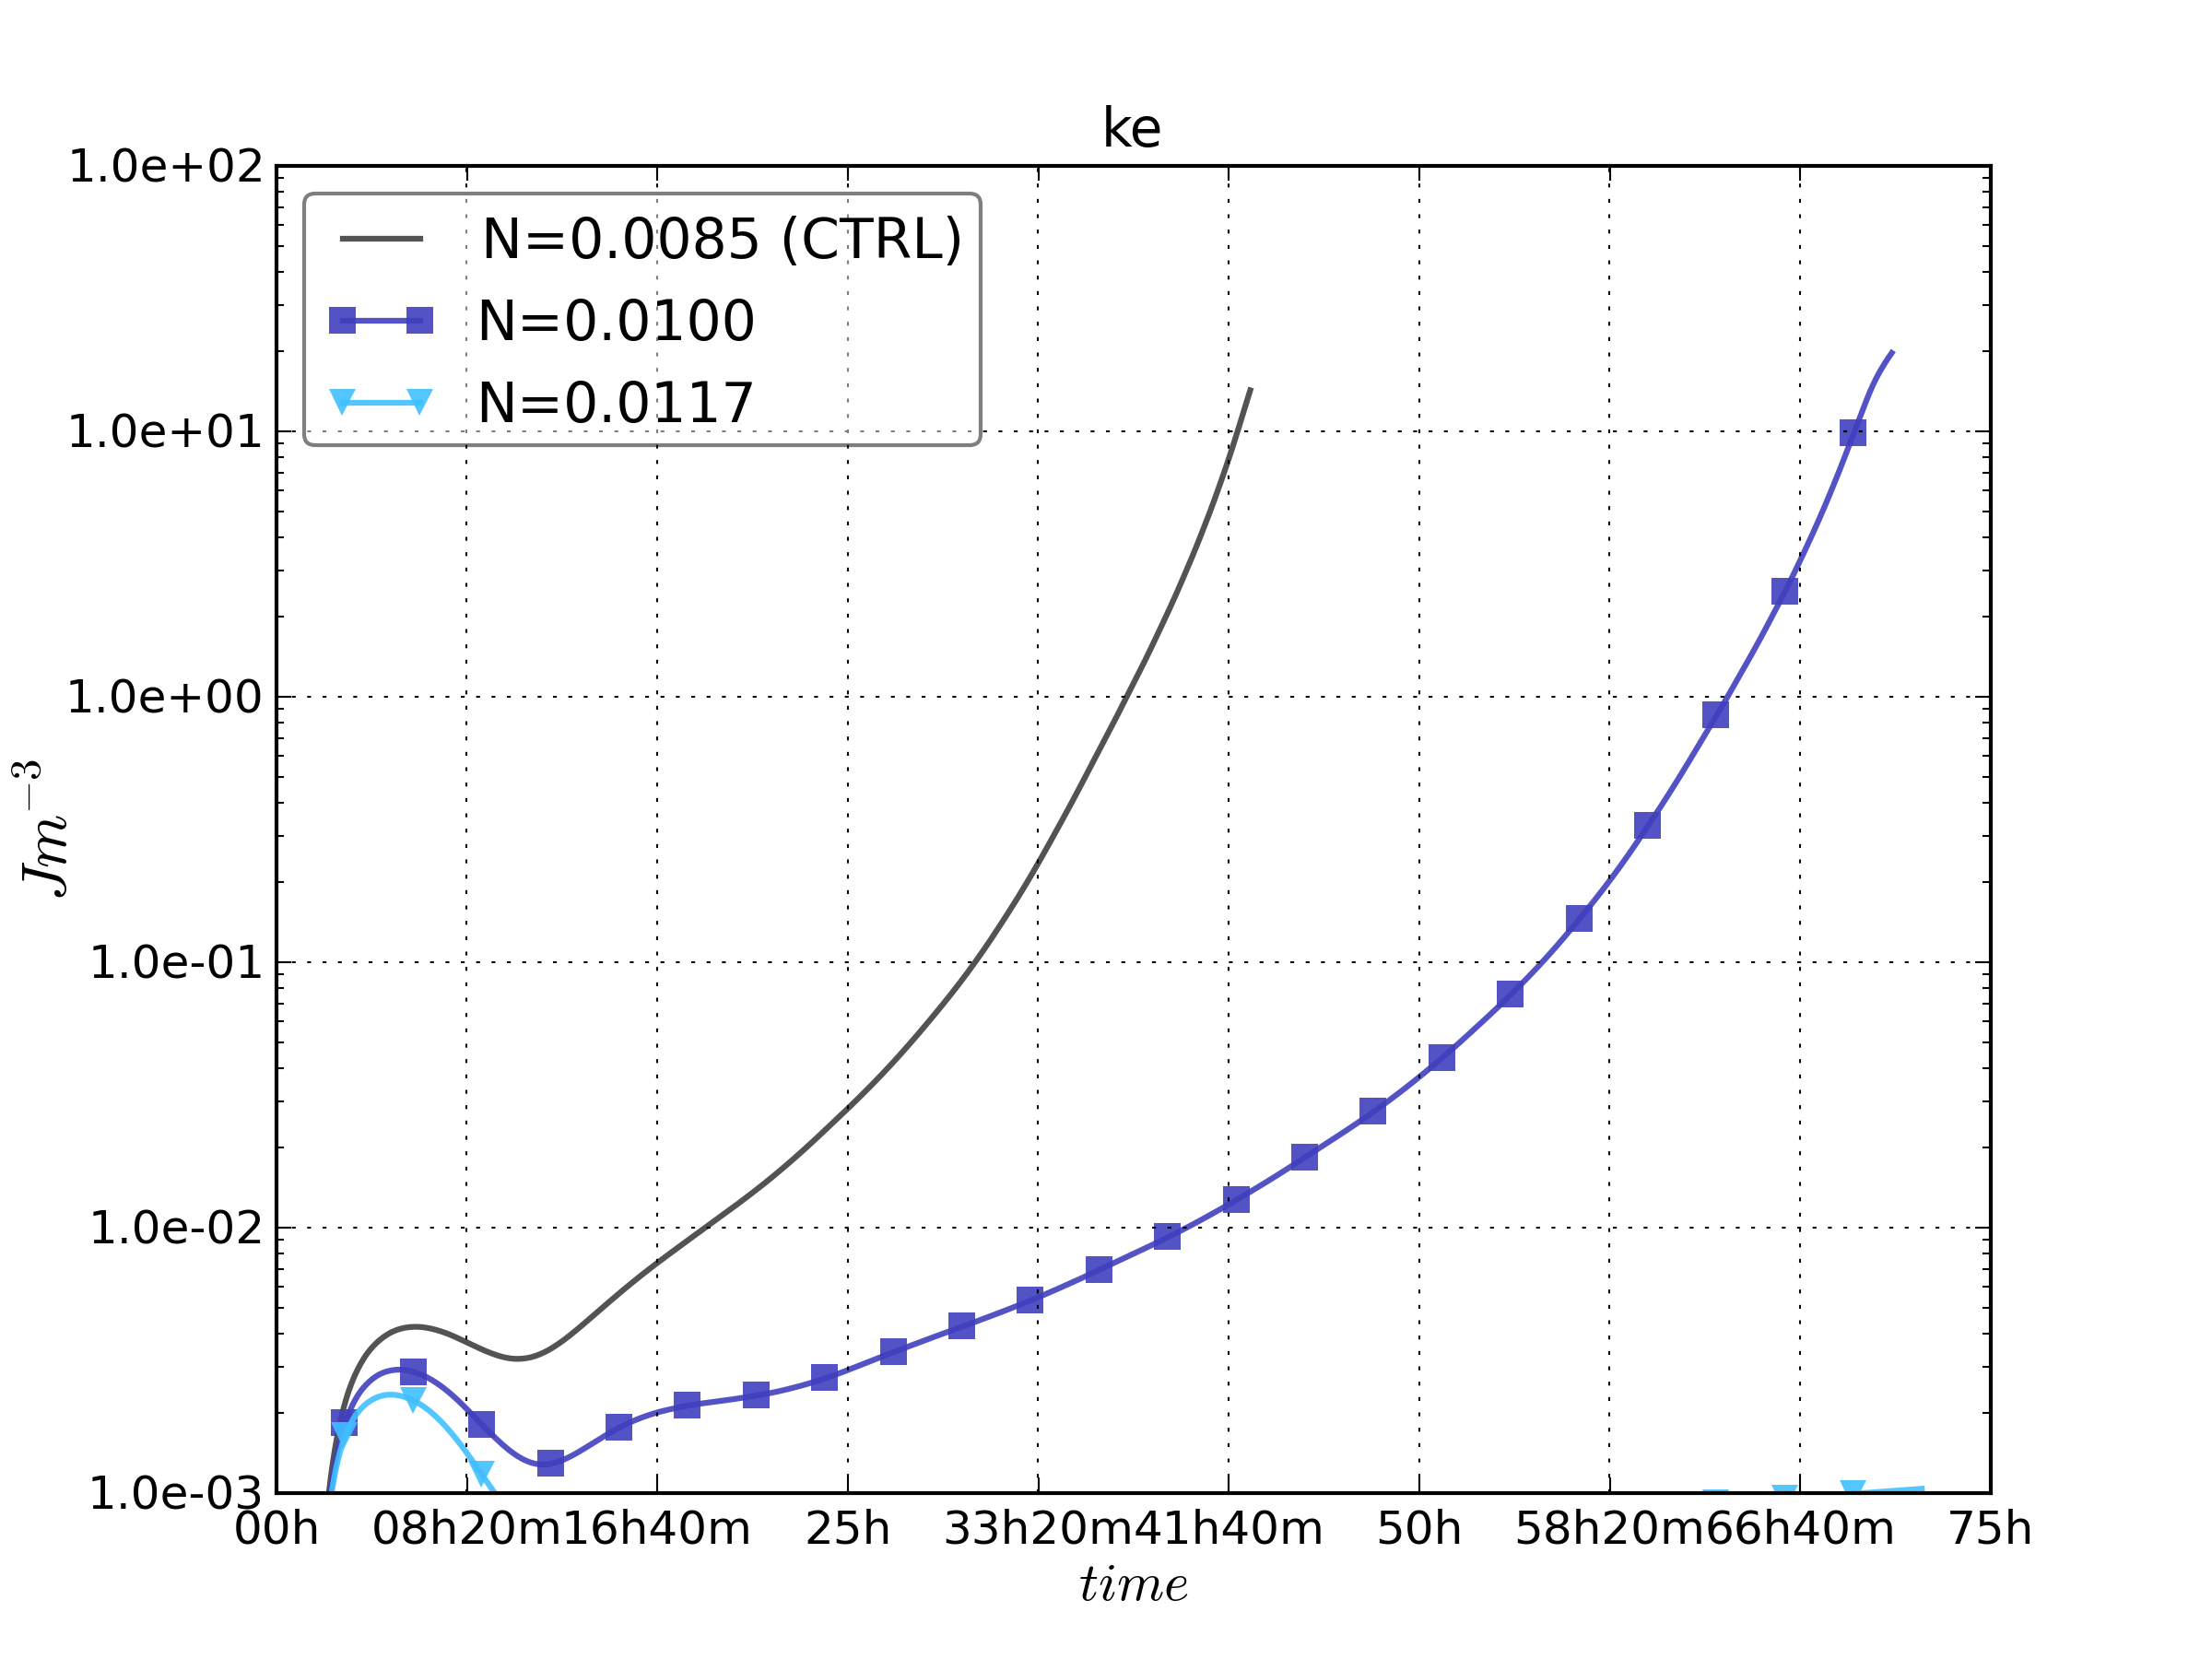
\includegraphics[width=\linewidth]{{./chapters/figures_results/ke.00h-72h.highN}.png}
%		\caption{ }
%        \label{fig:highN_ke}
%	\end{subfigure}
%	\hfill
%	\begin{subfigure}{0.45\textwidth}
%		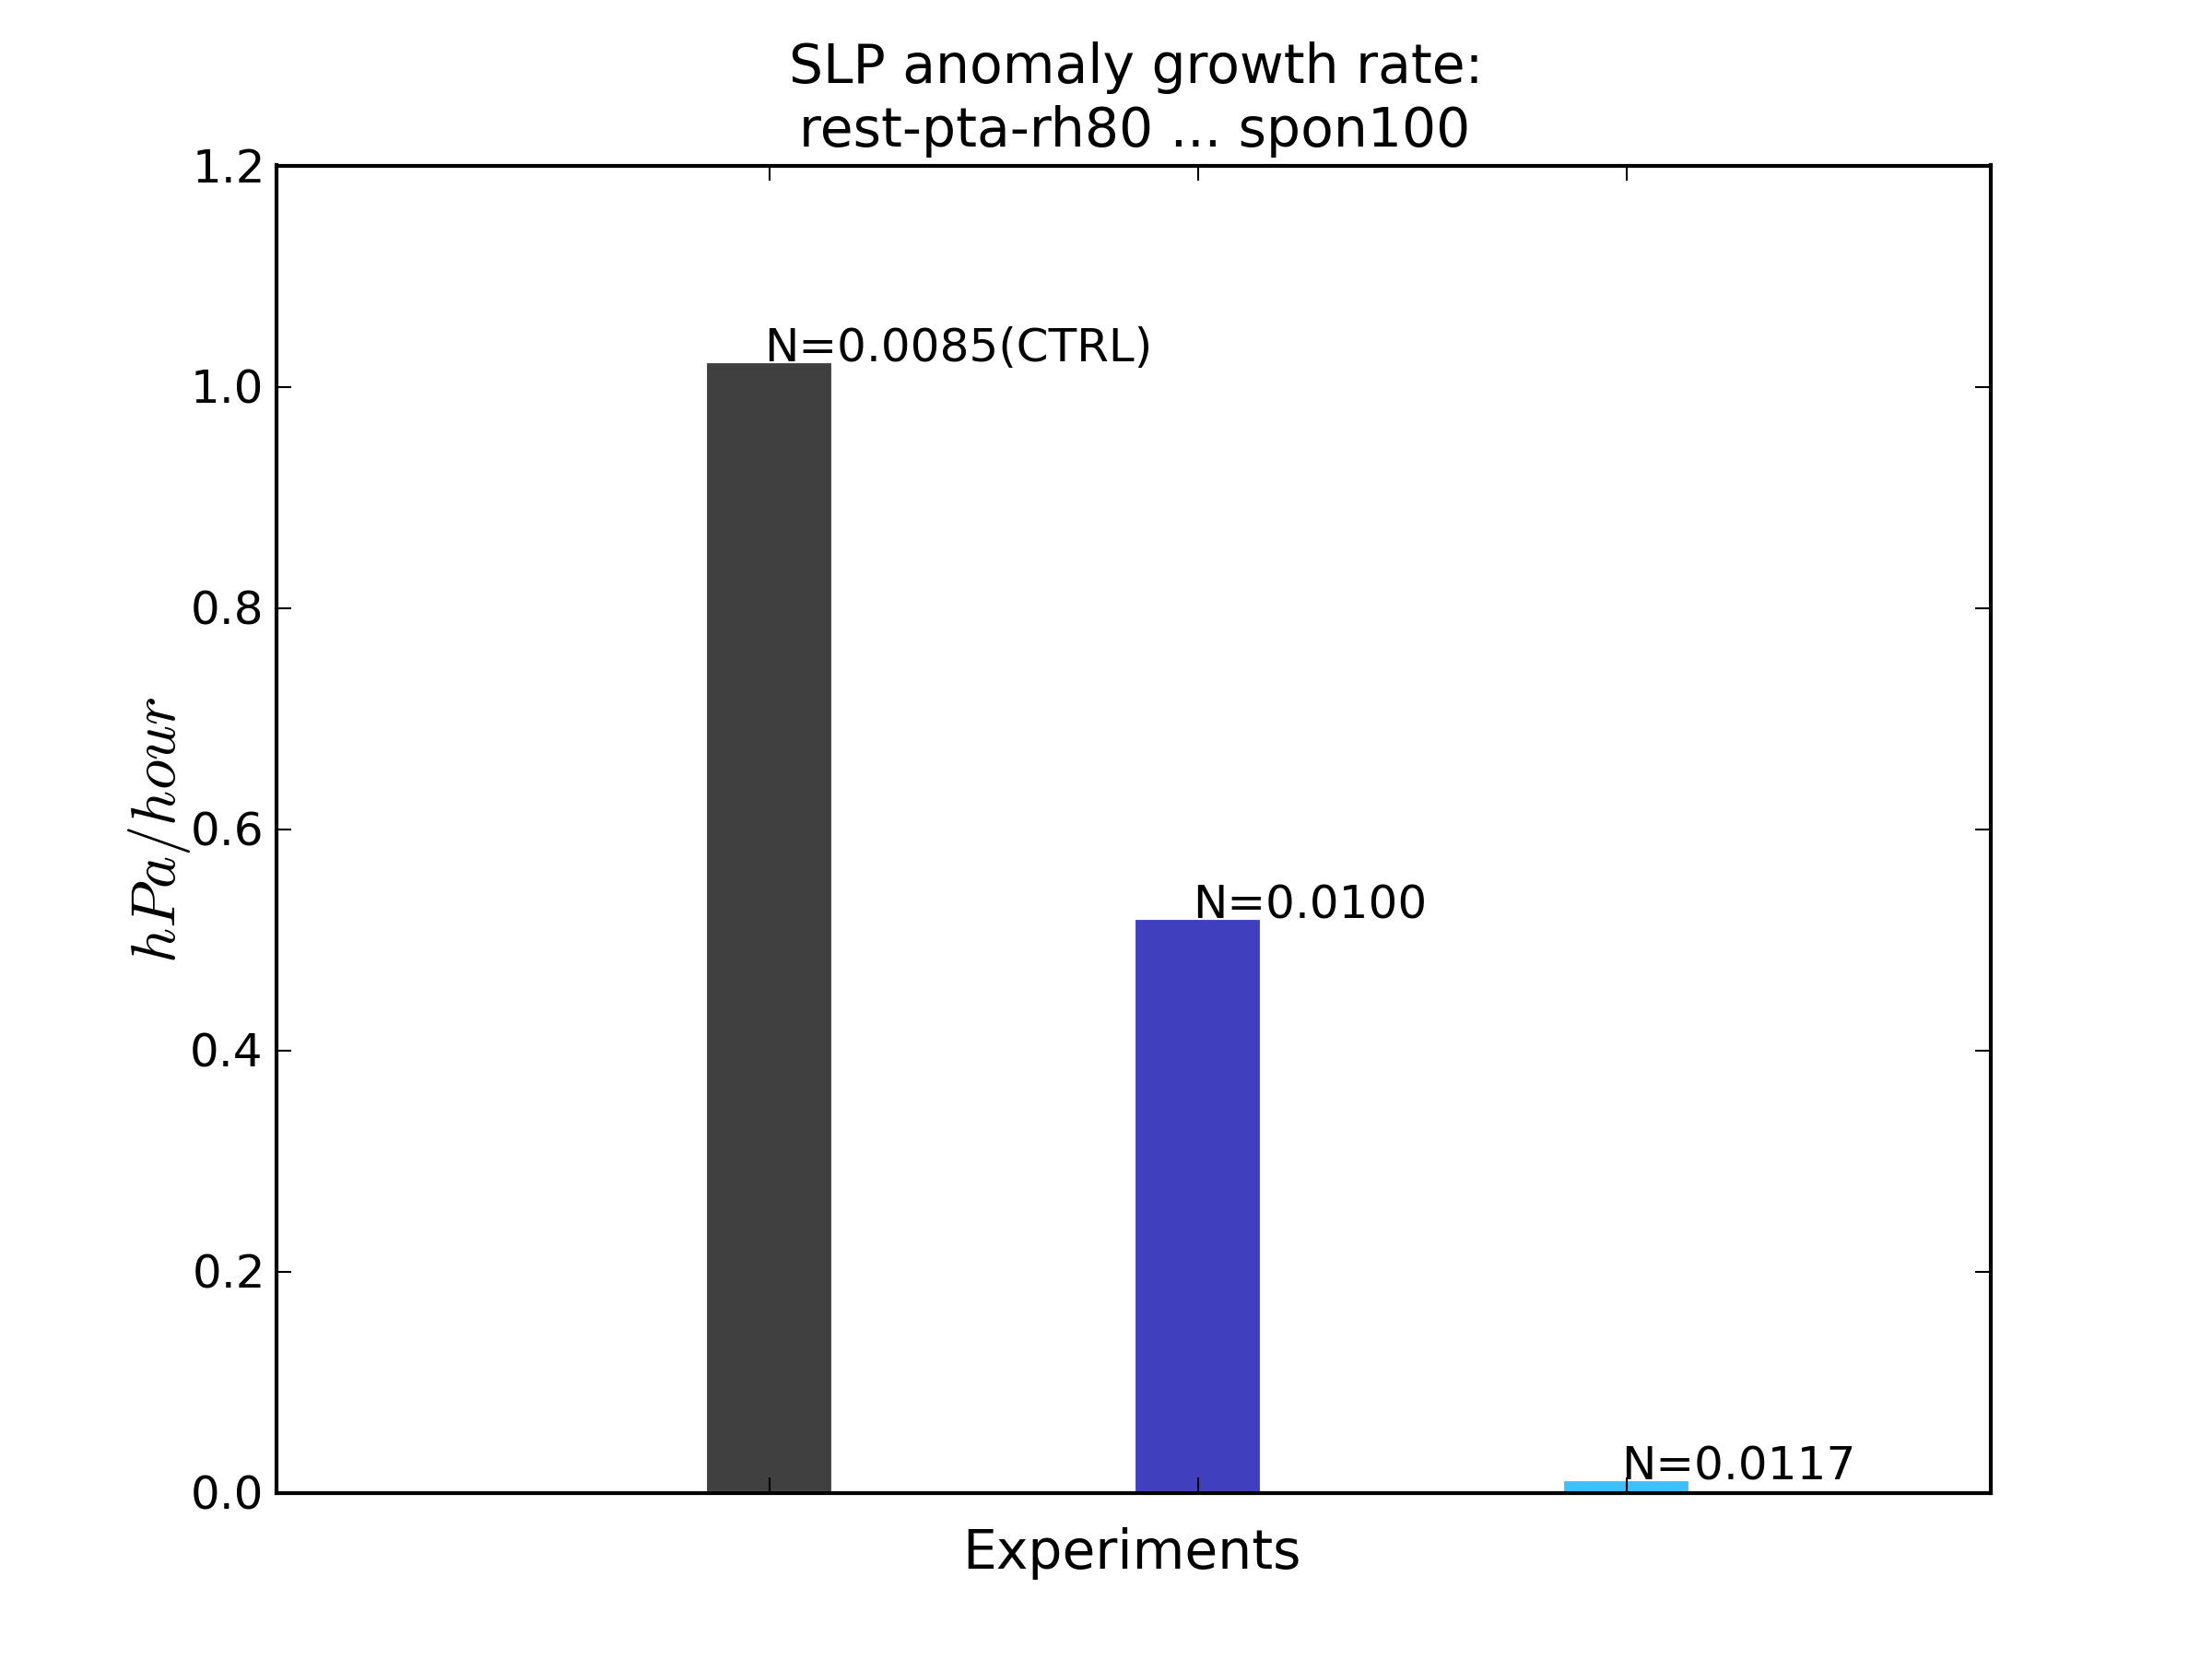
\includegraphics[width=\linewidth]{{./chapters/figures_results/slp_min_rate.00h-73h.highN}.png}
%		\caption{ }
%		\label{fig:highN_slp_rate}
%	\end{subfigure}
%        \caption{Эксперименты с пониженной устойчивостью фоновой атмосферы: изменение во времени кинетической энергии (слева) и чувствительность вихря к $N$ (справа).}
%\end{figure}
%
%На рис. \ref{fig:lowN_ke} представлена эволюция КЭ для экспериментов с пониженной статической устойчивостью относительно CTRL. Чтобы продлить время жизни вихря в этой группе экспериментов был уменьшен температурный контраст между воздухом и поверхностью воды за счет задания более высокой температуры атмосферы: $T_a=271\K$. Из-за этого развитие мезоциклона является более умеренным, чем в контрольном эксперименте, и кинетическая энергия даже в самом неустойчивом эксперименте лишь немного превышает $1\Jpm$. Более того, на основании рис. \ref{fig:lowN_ke} можно сказать, что стратификация $N\approx 0.0040\pers$ близка к критической для развития температурной аномалии: при $N>0.0040\pers$ рост КЭ не наблюдается. С точки зрения падения давления в центре вихря чувствительность интенсивности вихря к статической устойчивости показана на рис. \ref{fig:lowN_slp_rate}.
%
%Случай повышенной статической устойчивости рассматривается на примере экспериментов, в которых вертикальный градиент температуры равнялся $3\Kpkm$ ($N=0.0100\pers$) и $4\Kpkm$ ($N=0.0117\pers$). Рост КЭ в условиях более устойчивой стратификации ожидаемо оказывается слабее, чем в контрольном эксперименте, хотя после перемешивания нижних слоев атмосферы скорость роста в $N=0.0100\pers$  становится сравнима с контрольным. Сопоставление КЭ в трех экспериментов (рис. \ref{fig:highN_ke}) также обнаруживает наличие порогового значения для развития вихря. Таким образом, при разности температуры воды и воздуха $32\K$ (CTRL) и при градиенте температуры большем, чем $3\Kpkm$, выбранная амплитуда аномалии в 'сухой' атмосфере недостаточна для развития мощного мезоциклона.
%
%\subsection{Влияние устойчивости атмосферы на структуру атмосферных движений}
%Снижение статической устойчивости атмосферы отразилось не только на интегральных характеристиках, представленных выше, но и на пространственной динамике циклонической аномалии. Уже в первые часы модельного времени после инициализации температурного возмущения при разном $N$ волны, связанные с геострофическим (градиентным) приспособлением, имеют тем больше амплитуду и тем меньше фазовую скорость, чем меньше устойчивость. В этом можно убедиться на примере колебаний вертикальной скорости  $\tilde{w}$ в конкретной точке области (рис. \ref{fig:lowN_wfluct}).
%
%\begin{wrapfigure}{L}{0.5\textwidth}
%\begin{center}
%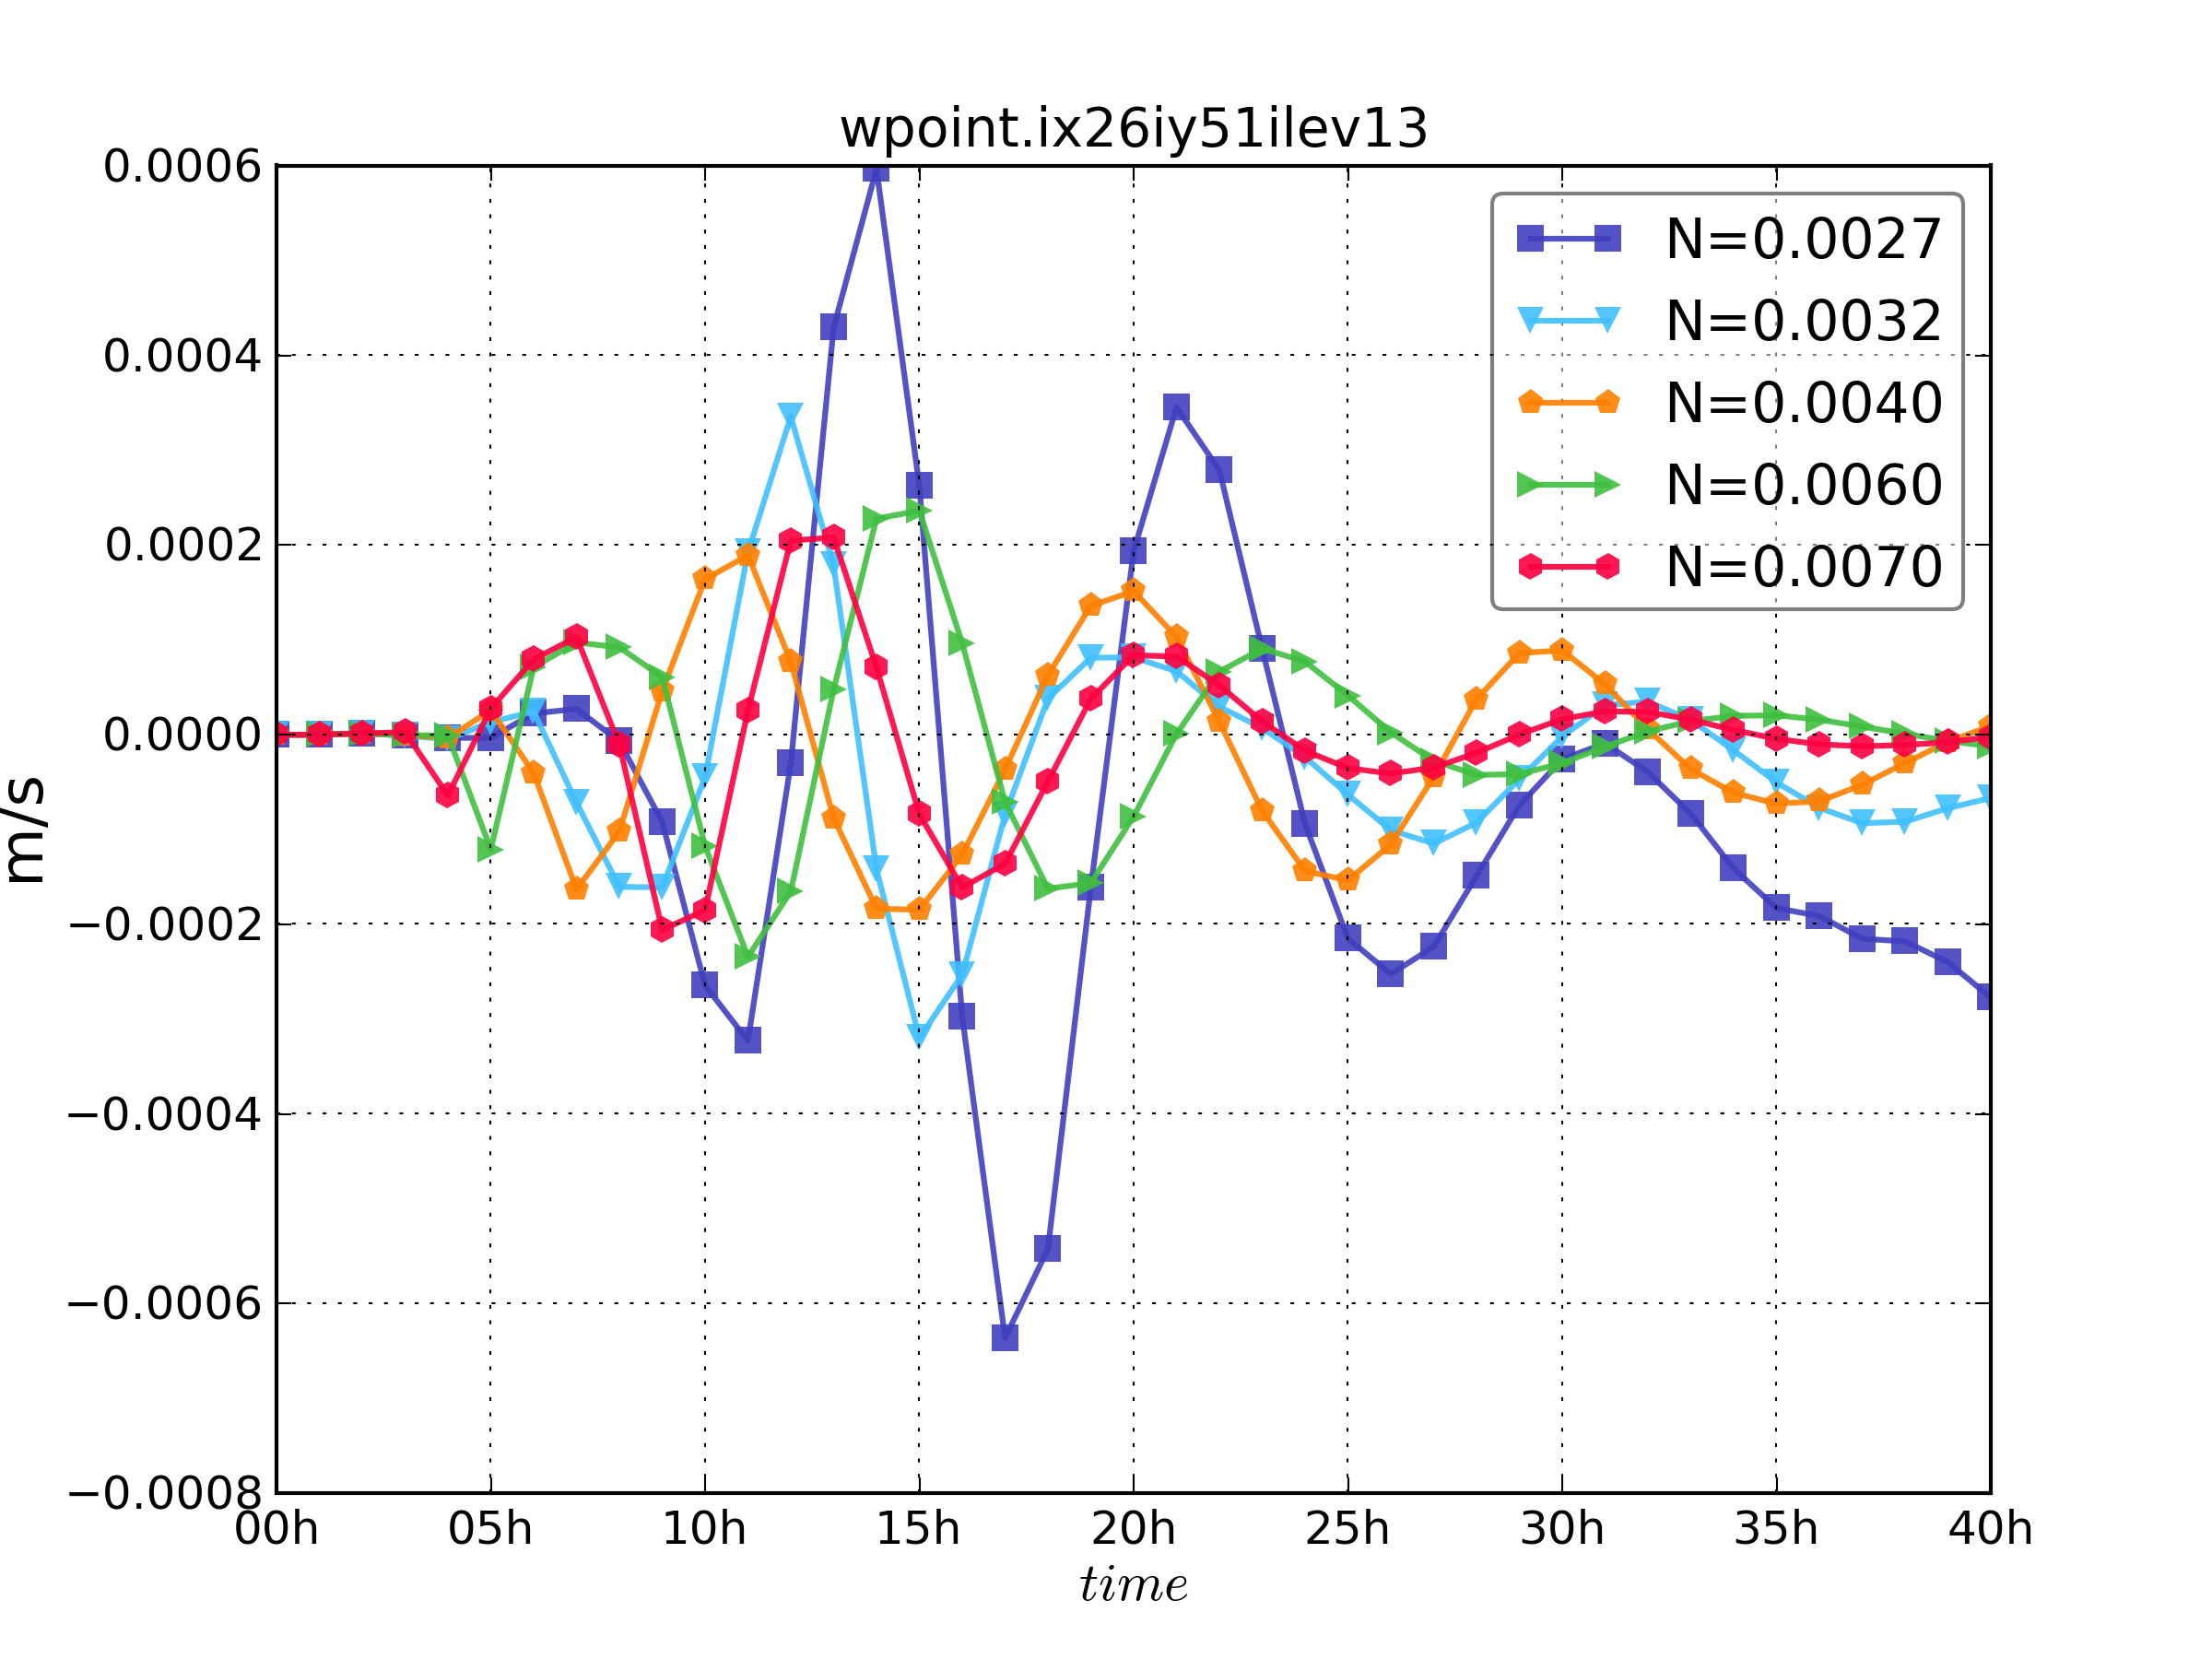
\includegraphics[width=\linewidth]{{./chapters/figures_results/wpoint.ix26iy51ilev13.00h-39h.stability}.png}
%\end{center}
%\caption{Колебания вертикальной скорости в точке ($r=250\km,p=300\hpa$) в экспериментах с разной фоновой стратификацией атмосферы.}
%\label{fig:lowN_wfluct}
%\end{wrapfigure}
%
%Горизонтальные разрезы вертикальной скорости показывают, что в экспериментах с самой низкой устойчивостью амплитуда инерционно-гравитационных волн на одном расстоянии от центра распределена не равномерно, а имеет четыре максимума, ориентированные к углам расчетной области. Данное обстоятельство говорит о неодинаковом поглощении излучаемых волн в буферной зоне модели и приводит к тому, в определенный момент четырехполюсная структура начинает преобладать, разделяя вихрь на четыре симметричные части, которые продолжают интенсифицироваться \ref{fig:lowN_hwind_split}. Напомним, что при повышенной устойчивости атмосферы в контрольном эксперимене вихрь разделялся на две части. Таким образом, при пониженной устойчивости (в данном случае при $N < 0.0060\pers$) развитие мезоциклона неустойчивым, а также становится более выгодно на мелких горизонтальных масштабах $L$.
%
%\begin{wrapfigure}{L}{0.5\textwidth}
%\begin{center}
%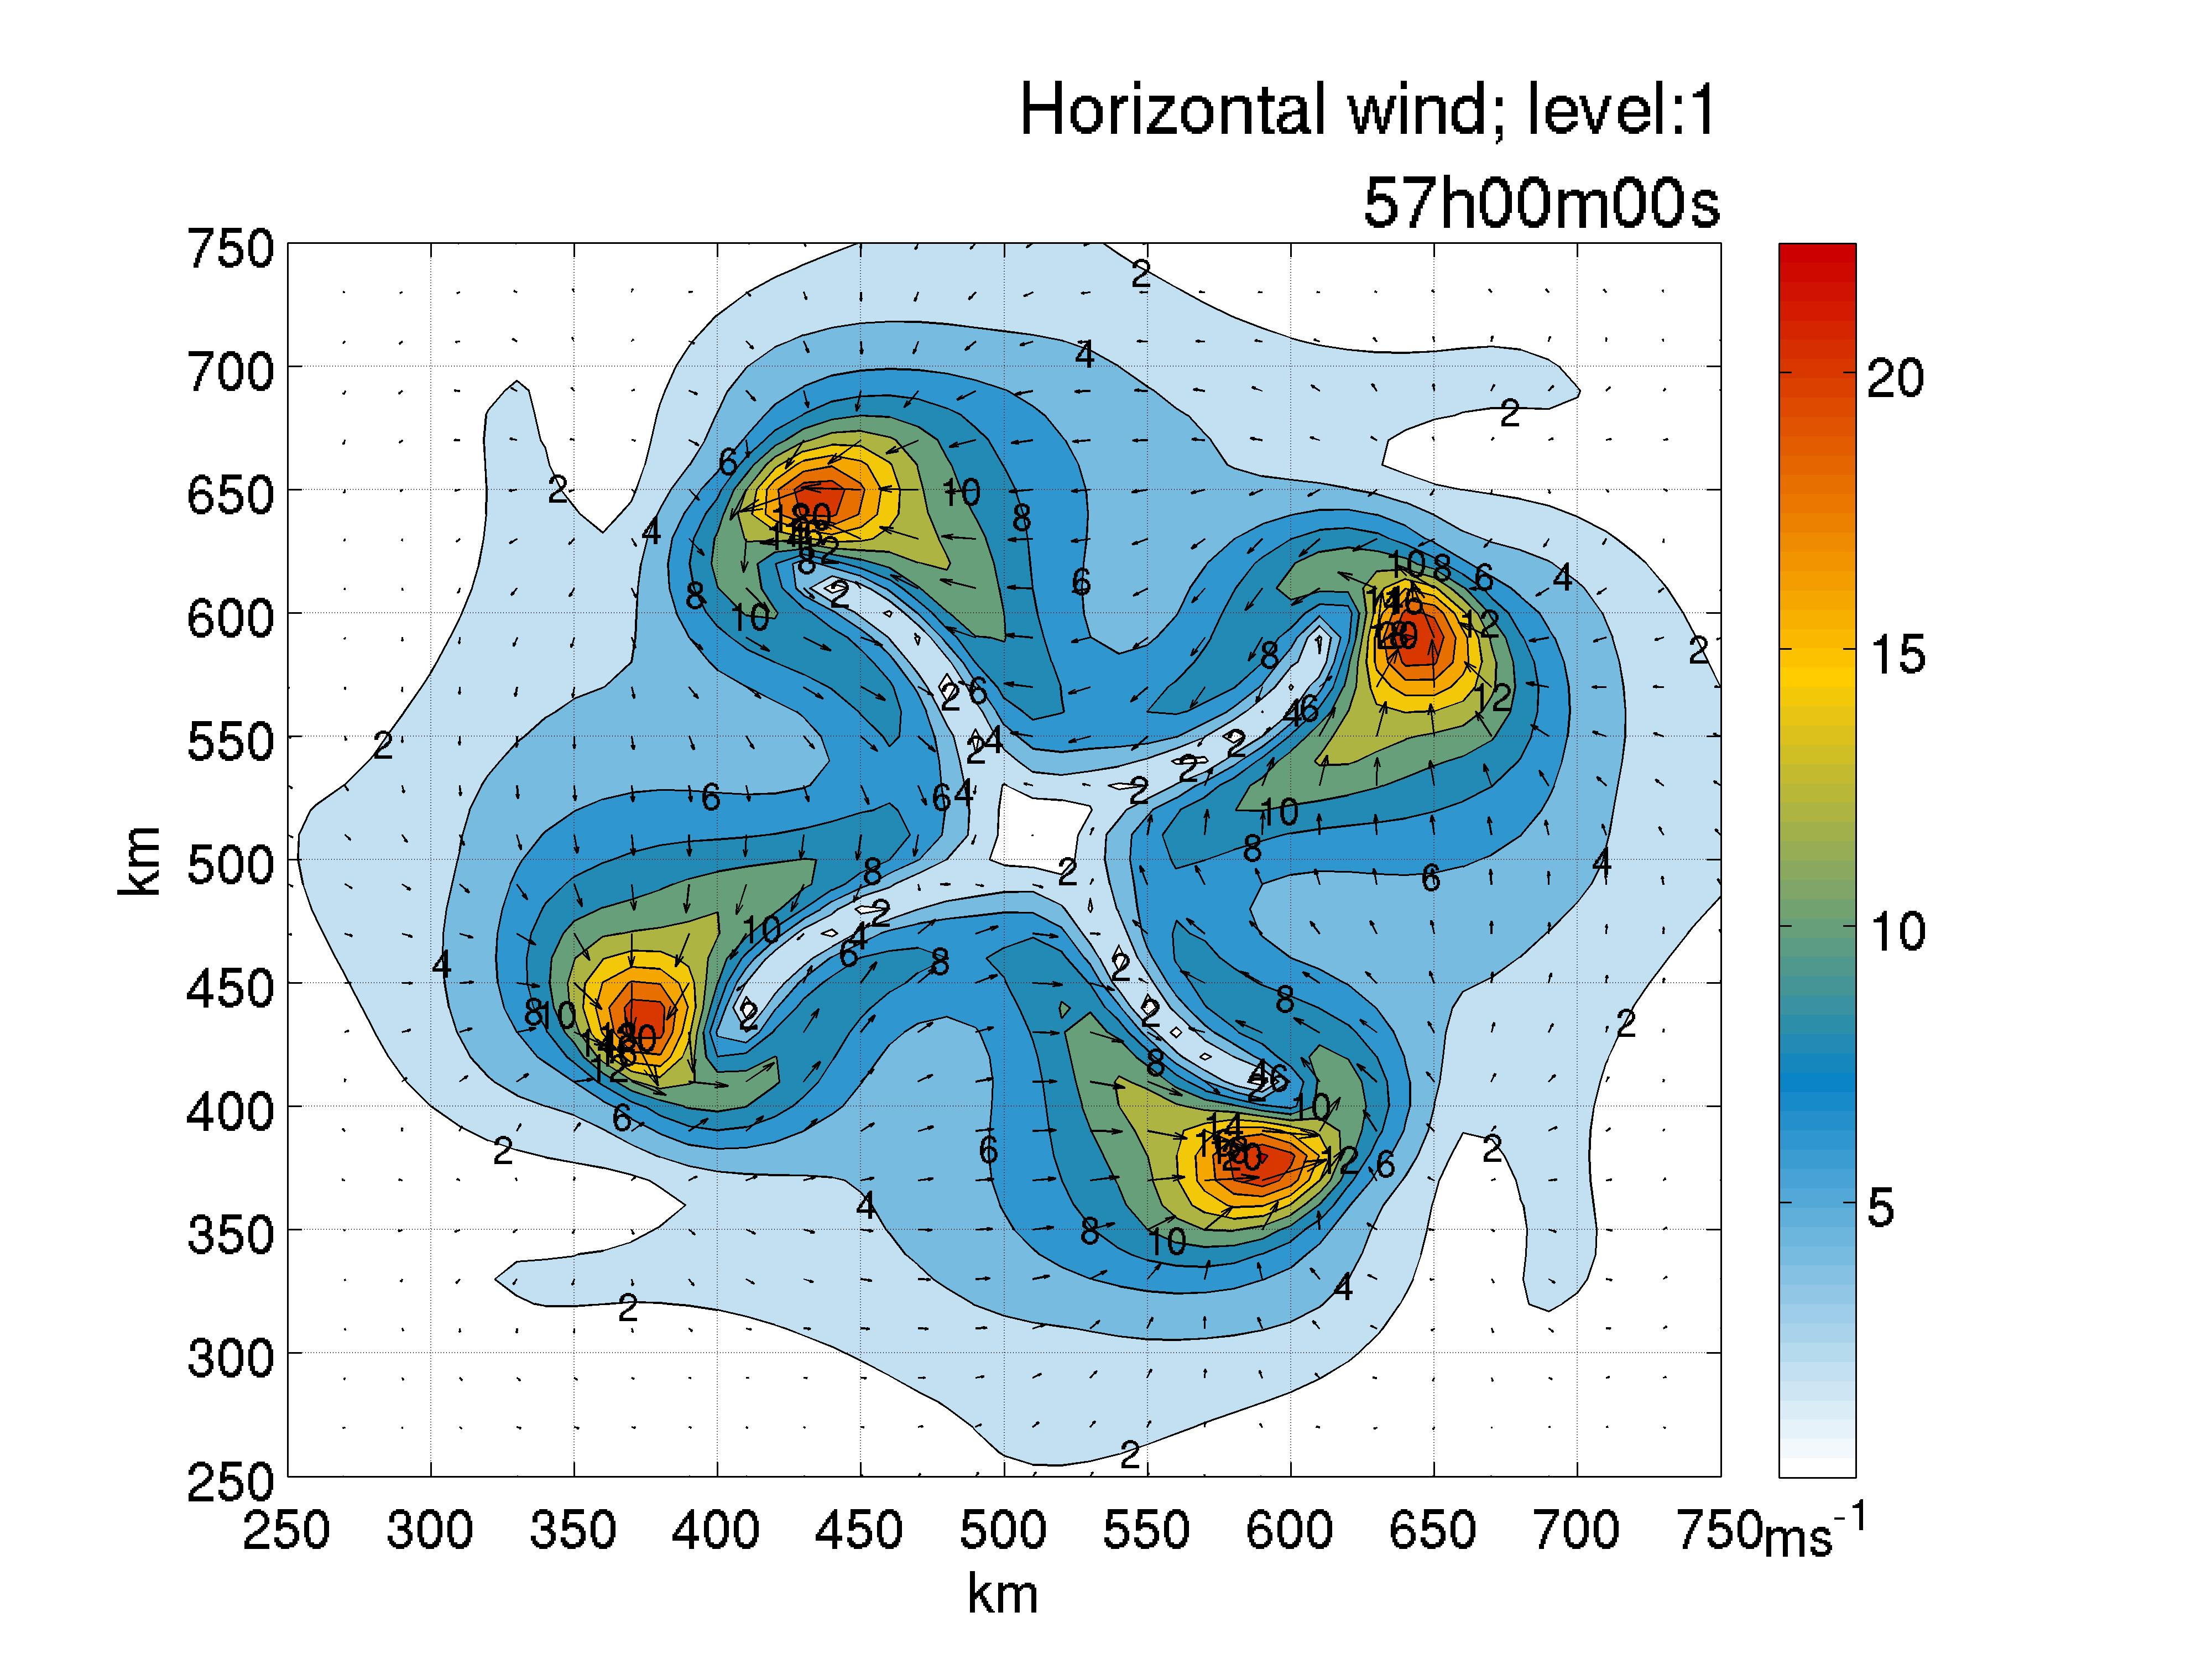
\includegraphics[width=\linewidth]{{./chapters/figures_results/VectorWind_p.x26-x76.y26-y76.ilev01.570000_lowN}.jpg}
%\end{center}
%\caption{Поле горизонтальной скорости ветра (область $500\times 500\km$). Эксперимент при $N=0.0027\pers$. 57 час модельного времени.}
%\label{fig:lowN_hwind_split}
%\end{wrapfigure}
%
%\section{Серия с разной температурой воды и воздуха}
%Выше были рассмотрена зависимость динамики вихря от таких характеристик фонового состояния атмосферы, как относительная влажность и статическая устойчивость. В них температура приводного слоя атмосферы равнялась $251\K$, а температура водной поверхности составляла $283\K$, создавая значительный вертикальный градиент температуры между водой и воздухом. В реальной атмосфере настолько большой градиент температуры достигается нечасто \citep{ForbesLottes1985}, поэтому были поставлены эксперименты, в которых разность температуры $\Delta T$ меняется от $12$ до $29\K$ за счет увеличения температуры всей толщи атмосферы или уменьшения температуры поверхности океана. 
%
%Если проанализировать эволюцию кинетической энергии (\ref{}) для экспериментов с одной и той же ТПО ($283\K$), но разной температурой атмосферы, то можно увидеть, что величина и скорость роста кинетической энергии пропорциональна разнице температур на границе вода-воздух, причем данная зависимость нелинейная: при малых значениях $\Delta T$ отличия между экспериментами менее заметны. Этот факт подтверждается зависимостью интенсивности циклона от $\Delta T$ и соответствующей таблицей \ref{}, в которой управляющим параметром чувствительности является $\Delta T$.
%
%Теперь вместо температуры воды зафиксируем параметр $\Delta T$, а температуру воздуха и воды изменим и опять же обратимся к ходу кинетической энергии на рис. \ref{} и \ref{}. На первом из этих рисунков сравнивается несколько экспериментов с $\Delta T=20\K$, на втором разность составляет $\Delta T=26\K$. Хорошо видно, что кривые на каждом из графиков почти не отличаются друг от друга. Из этого следует интуитивно понятный вывод, что динамика полярных мезоциклонов гораздо больше зависит от разности температур поверхности и атмосферы, чем от температуры поверхности самой по себе (в отличие от тропических циклонов \citep{EmanuelRotunno1989}). Схожие оценочные эксперименты проводились авторами \citep{YanaseNiino2007}, и ими было выяснено что чувтствительность вихря к средней температуре воды и воздуха (при фиксированной разнице) также невелика. Однако в экспериментах в указанной статье чувствительность к температуре обнаруживает зависимость от степени бароклинности атмосферы: чем меньше сдвиг ветра, тем больше чувствительность. По-видимому, это связано с тем, что при увеличении бароклинности фоновой атмосферы в бюджете кинетической энергии растет доля бароклинного слагаемого (аналогичного $C(A,K)$), а роль остальных факторов уменьшается.
%
%\section{Потоки тепла с поверхности}
%Многие особенности развивающегося вихря, описанные в предыдущих разделах, указывают на то, что в его динамике наиболее велика роль процессов при взаимодействии с подстилающей поверхностью, а именно турбулентных потоков явного и скрытого тепла. 
%
%В настоящем разделе подводятся результаты нескольких серий экспериментов, в которых потоки тепла и импульса с поверхности были отключены или искусственно изменены. Как уже было сказано в пункте \ref{sec:exp:surfpar}, эти эксперименты позволят с уверенностью говорить о роли потоков с поверхности в динамике вихря, а также о том, какой механизм доминирует в эволюции вихря.
%
%\subsection{Эксперименты без потоков явного и скрытого тепла в приводном слое}
%\label{sec:res:nohle}
%
%
%\begin{figure}[h]
%	\centering
%	\begin{subfigure}{0.45\textwidth}
%		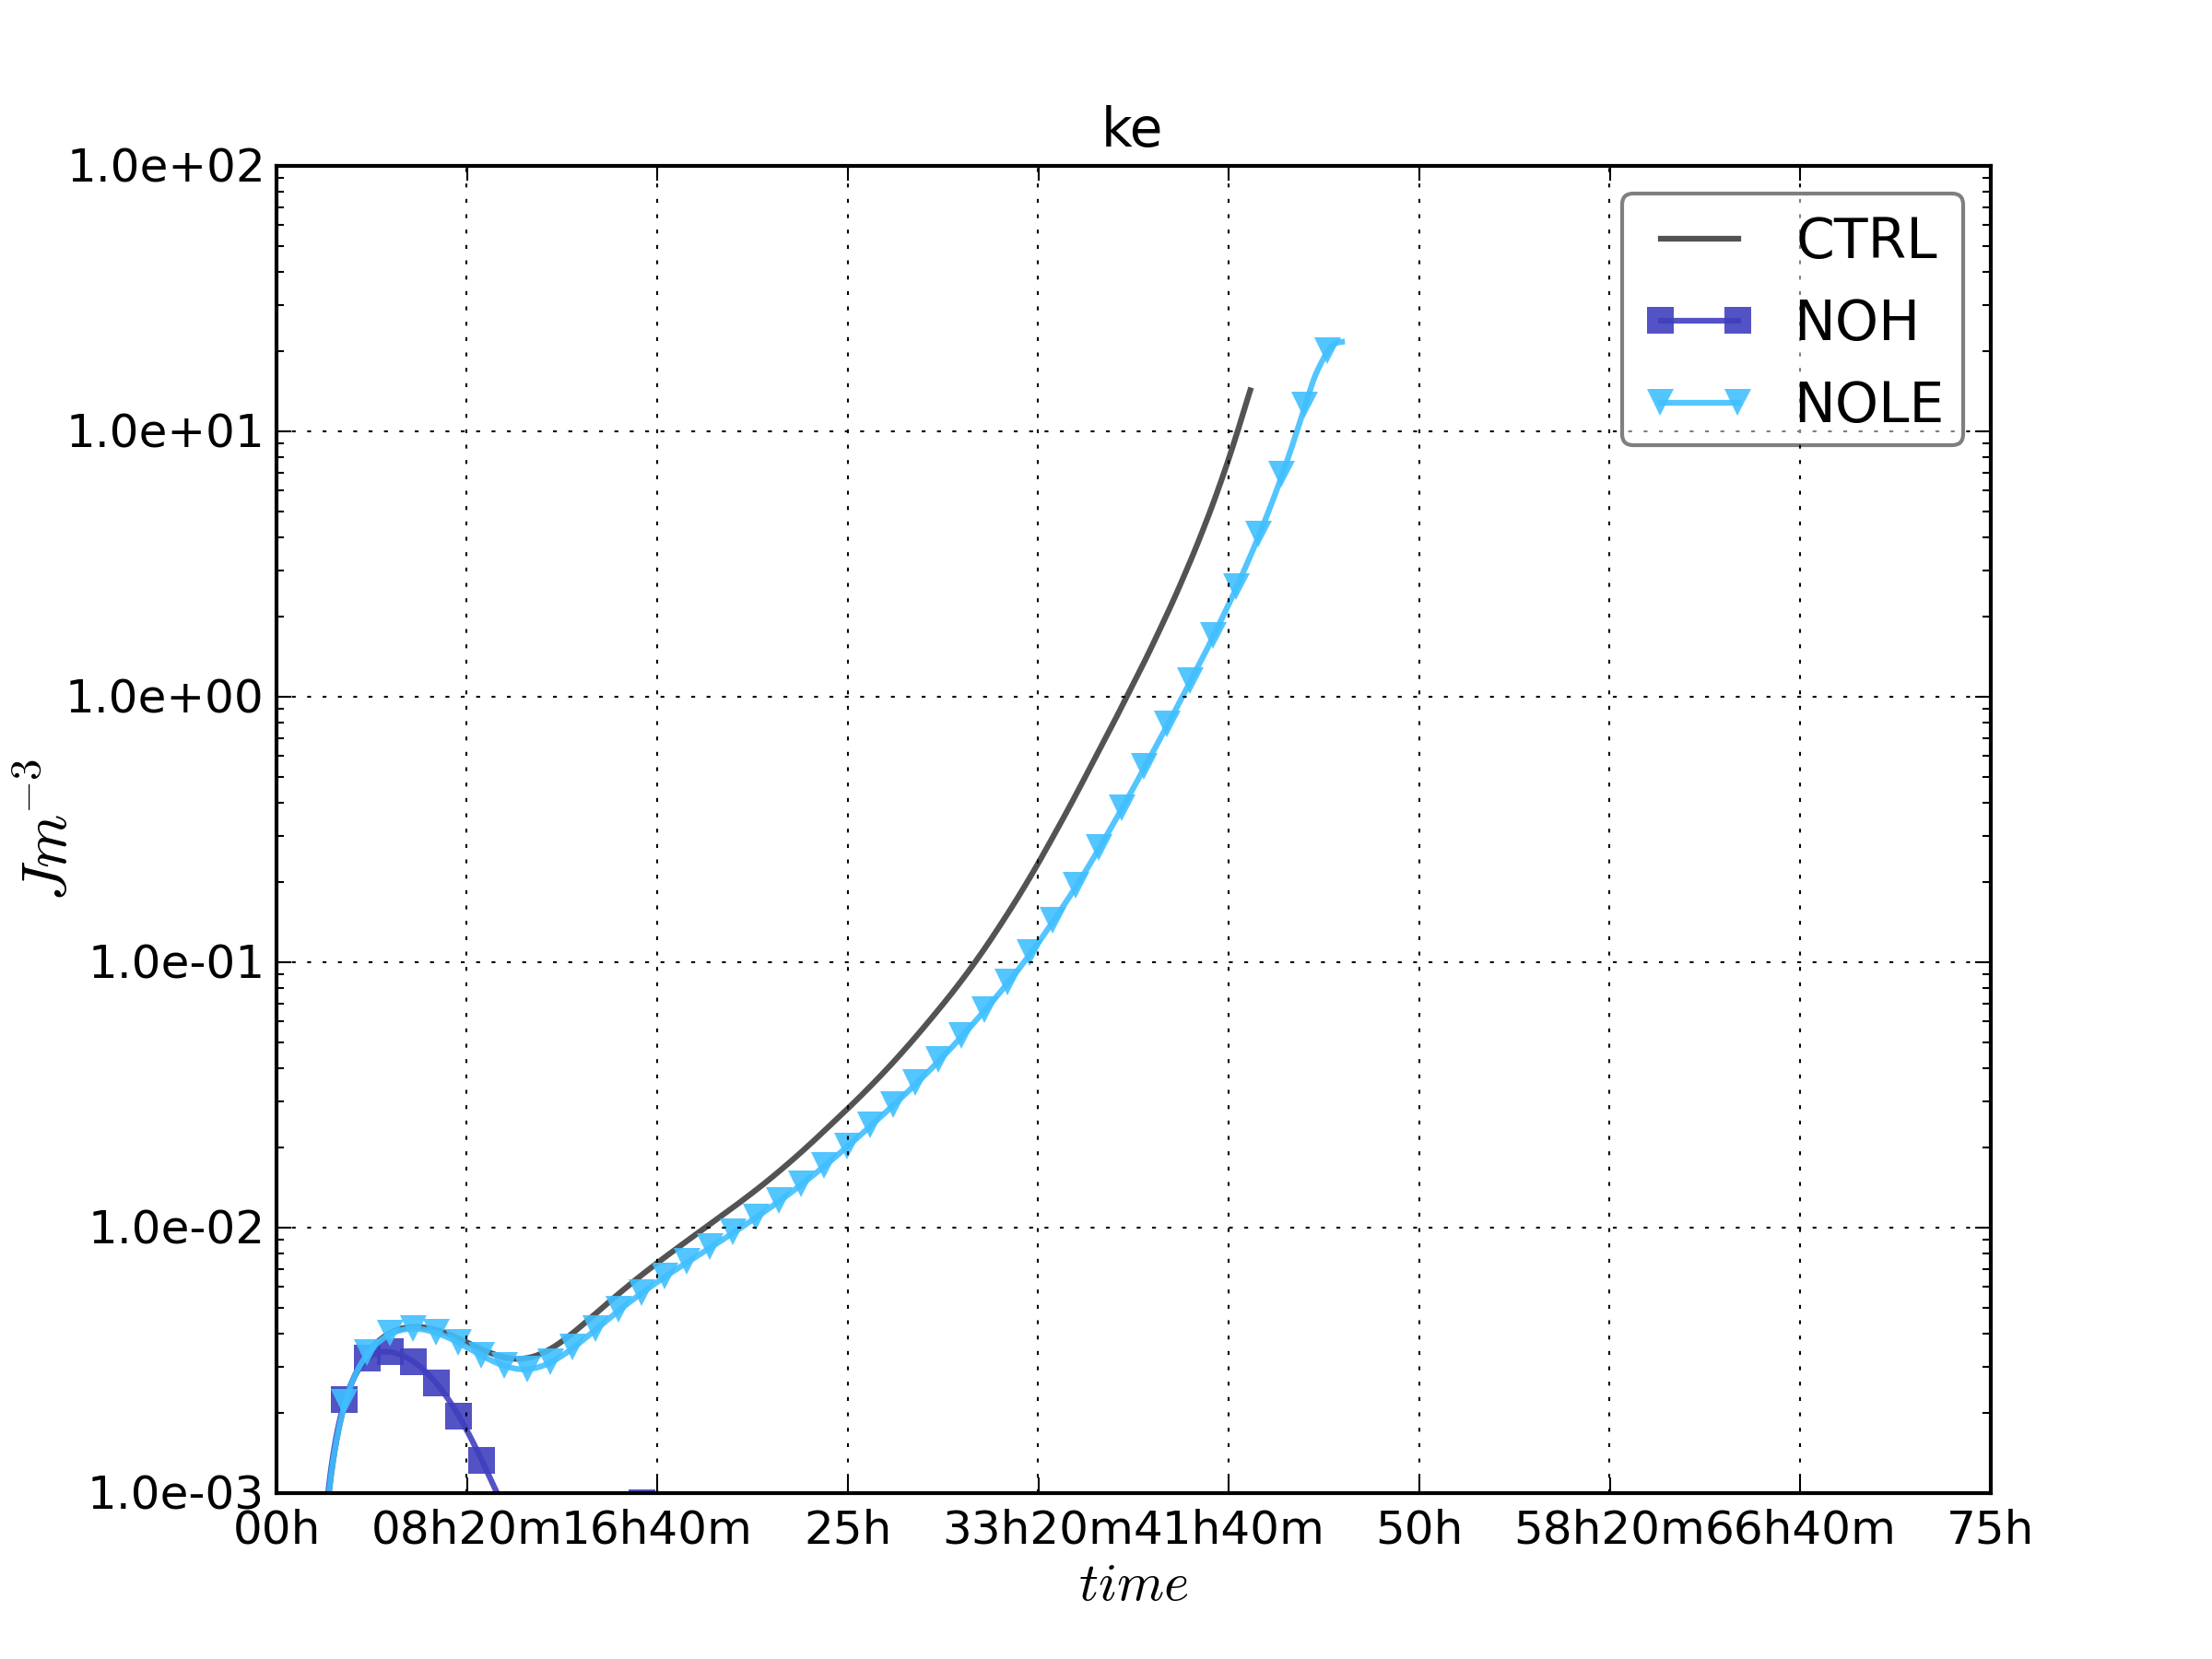
\includegraphics[width=\linewidth]{{./chapters/figures_results/ke.00h-72h.nohle}.png}
%		\caption{ }
%        \label{fig:nohle_ke}
%	\end{subfigure}
%	\hfill
%	\begin{subfigure}{0.45\textwidth}
%		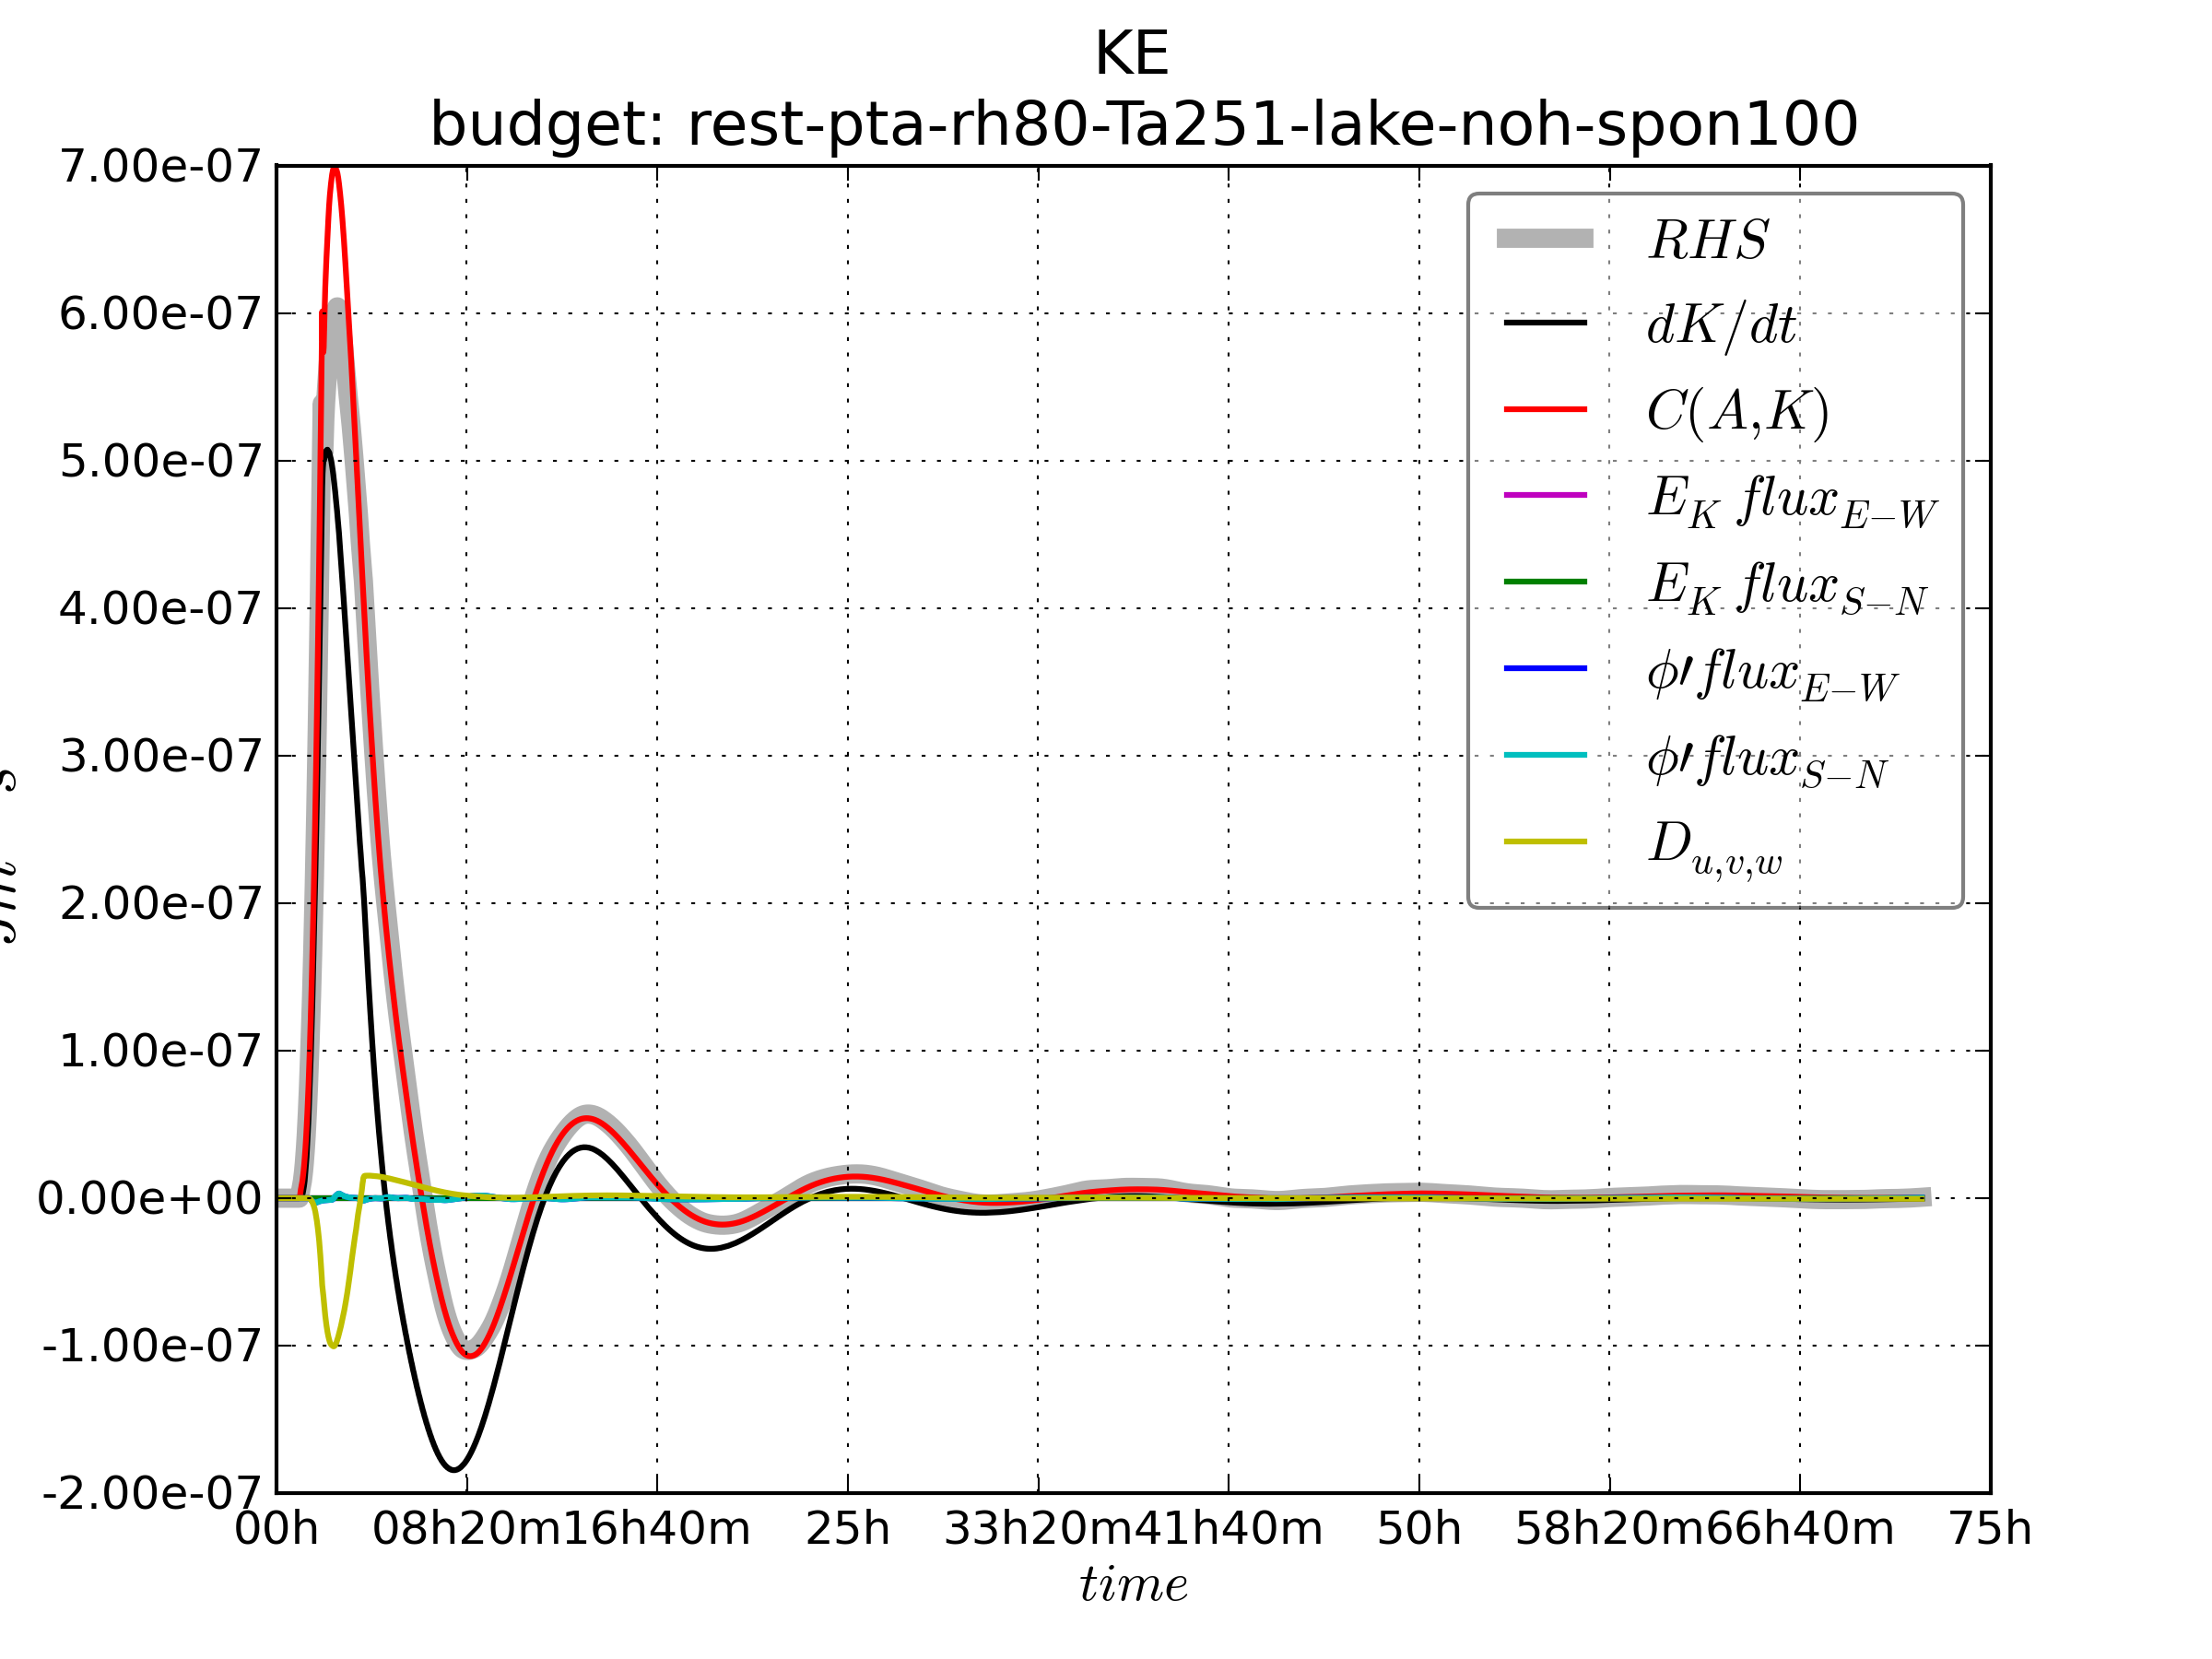
\includegraphics[width=\linewidth]{{./chapters/figures_results/rest-pta-rh80-Ta251-lake-noh-spon100.dkdt}.png}
%		\caption{ }
%		\label{fig:noh_dkdt}
%	\end{subfigure}
%        \caption{Эволюция кинетической энергии в экспериментах с отключенными потоками тепла (NOH) и влаги (NOLE) в приводном слое по сравнению с контрольным экспериментом (слева) и бюджет кинетической энергии в эксперименте NOH (справа).}
%\end{figure}
%
%Как будет развиваться начальная температурная аномалия в чисто адиабатической атмосфере --- без притока тепла от фазовых переходов воды и без турбулентных потоков с поверхности? Резонно предположить, что для интенсификации вихря их будет не хватать, особенно это касается потоков тепла с поверхности. Убедиться в этом можно по результатам экспериментов NOH, NOLE, NOHLE, в которых в модели были отключены соответственно потоки явного или скрытого тепла и оба потока одновременно. Представленная на рис. \ref{fig:nohle_ke} эволюция кинетической энергии мало отличается в эксперименте NOLE. В эксперименте NOH после возникновения перехода части ДПЭ (запасенной в начальной аномалии) в КЭ и формирования слабой циклонической циркуляции, рост кинетической энергии постепенно прекращается \ref{fig:noh_dkdt}. Заметим, что полностью вихрь не исчезает (согласуется с теорией, изложенной в \citep{RT2003}), а КЭ остается на уровне $10^{-4}\Jpm$. 
%
%\subsection{Эксперименты с разными параметризациями потоков тепла}
%\begin{wrapfigure}{r}{0.5\textwidth}
%\begin{center}
%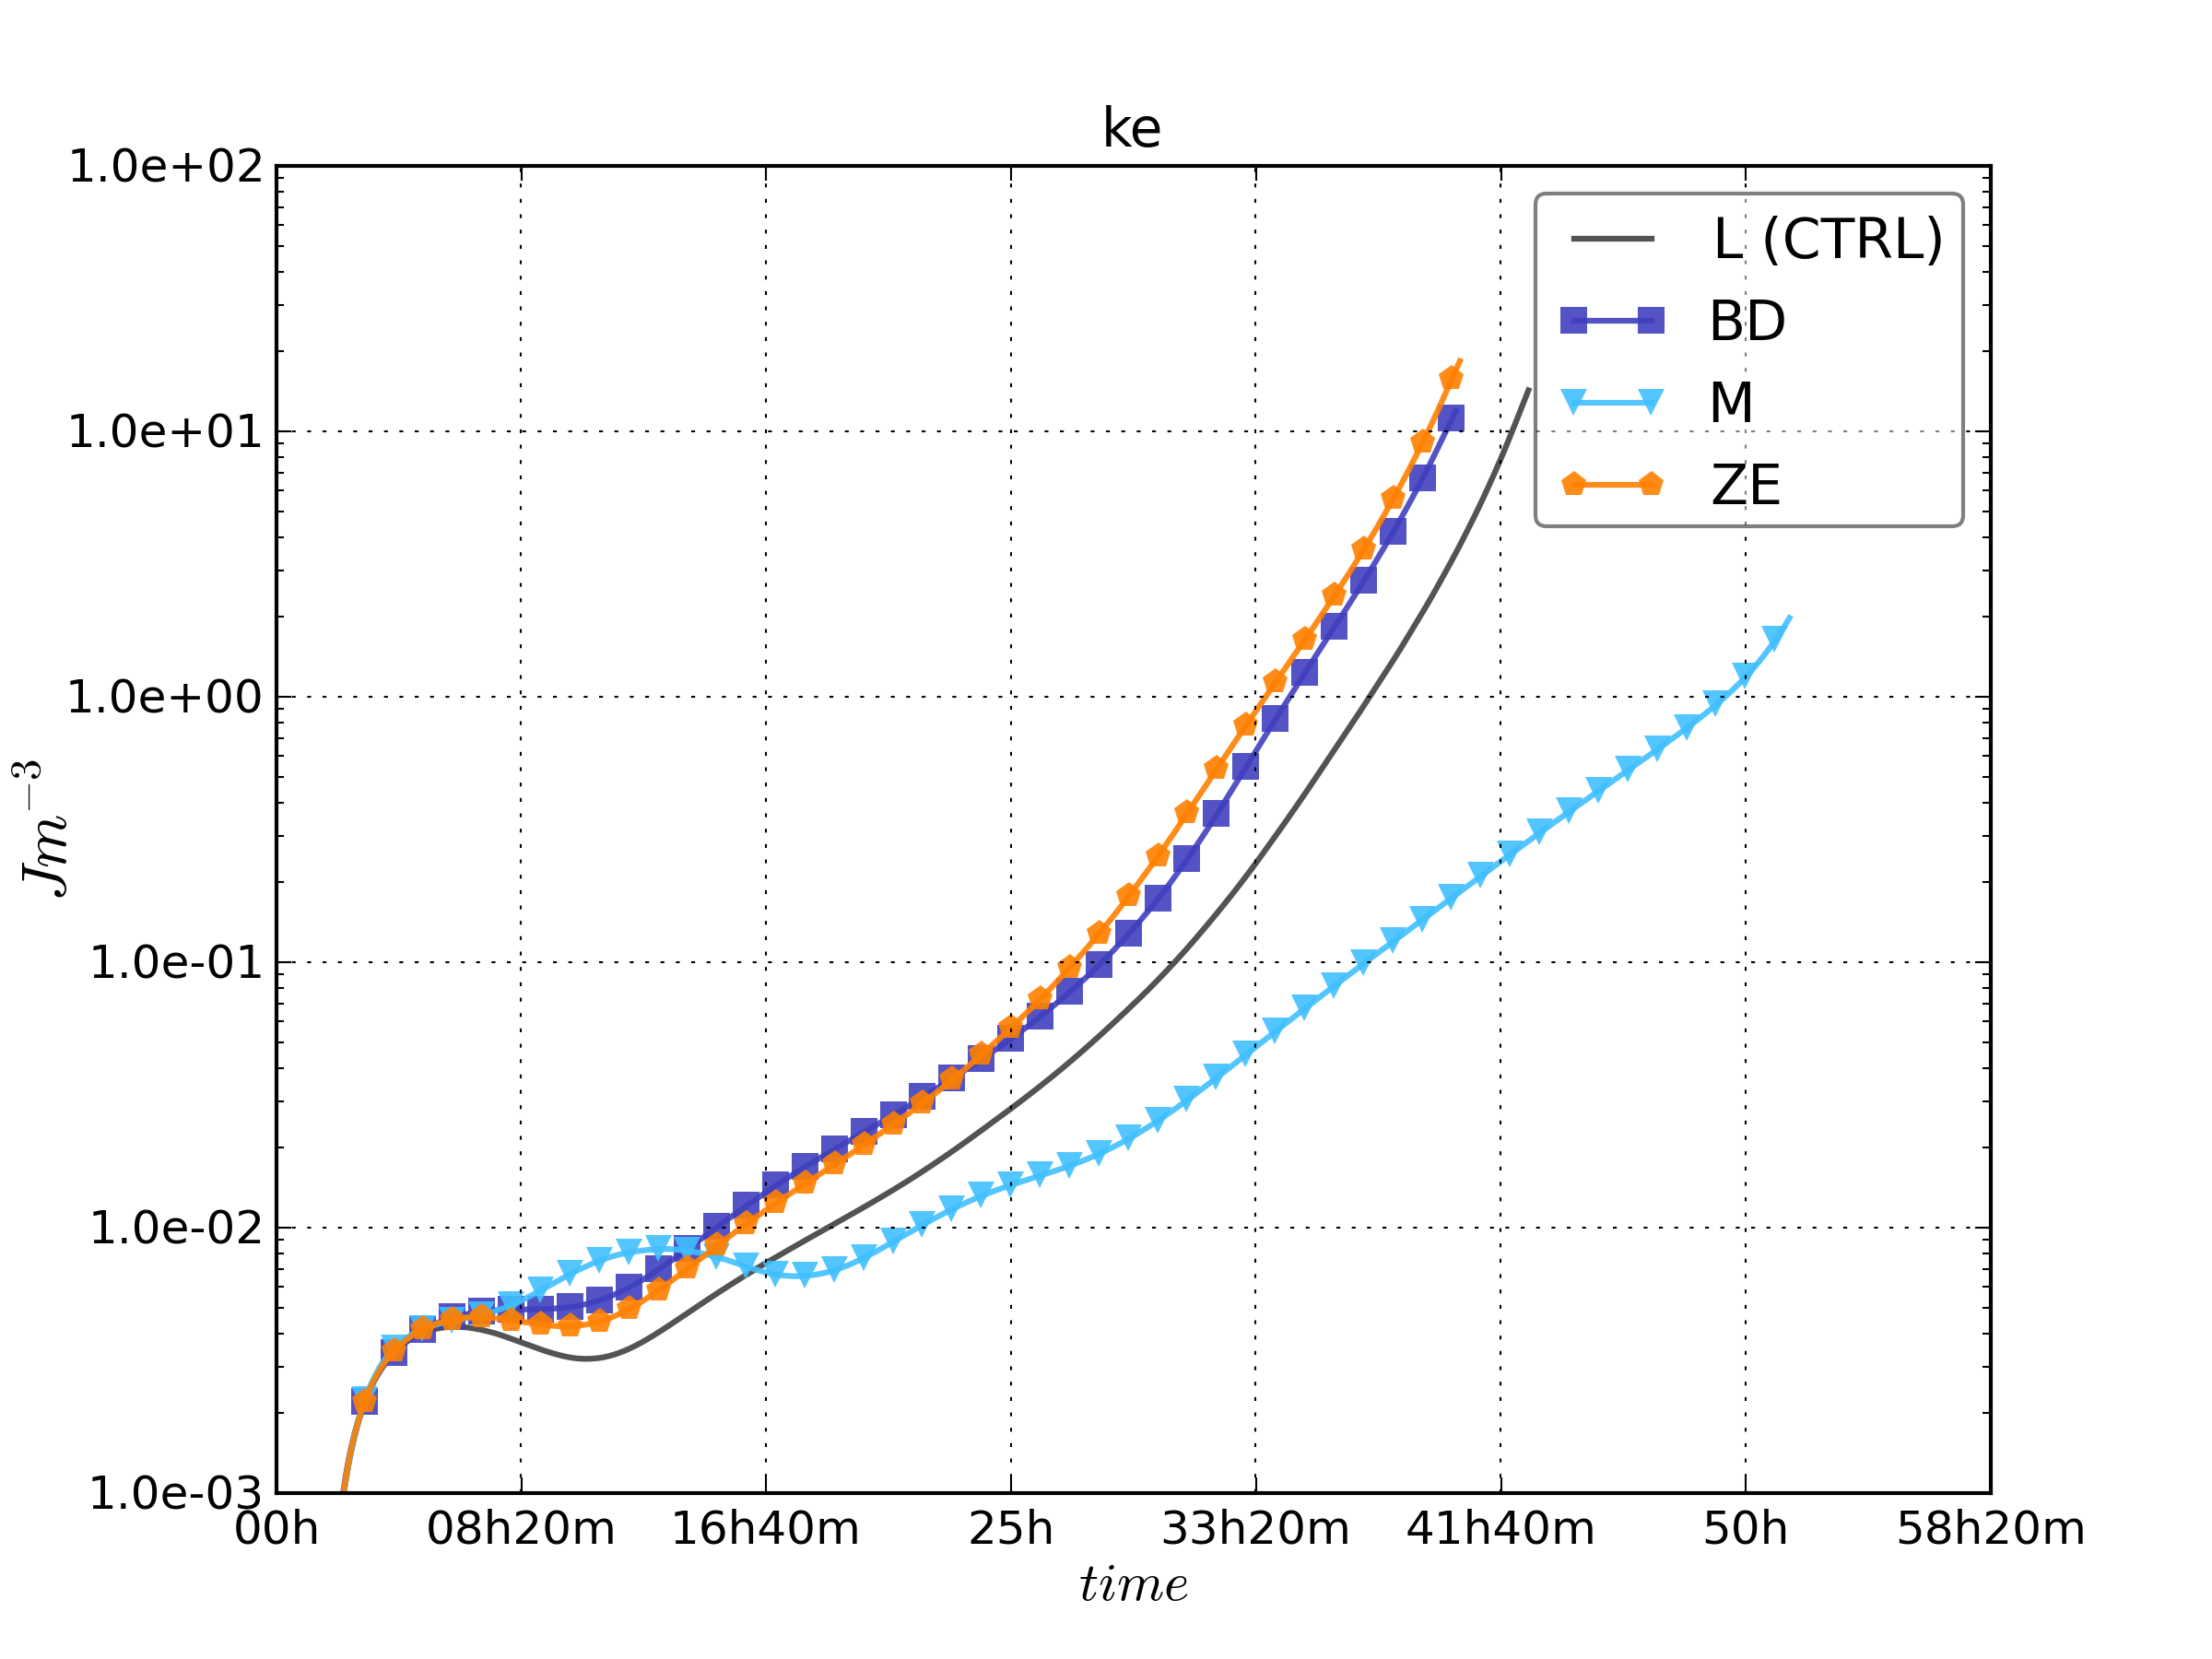
\includegraphics[width=\linewidth]{{./chapters/figures_results/ke.00h-51h30m.surfpar}.png}
%\end{center}
%\caption{Эволюция кинетической энергии в экспериментах с параметризациями BD, M, ZE турбулентных потоков в приводном слое по сравнению с контрольным экспериментом (L)}
%\label{fig:surfpar_ke}
%\end{wrapfigure}
%Начнем с того, что сравним результаты расчетов, сделанных с использованием разных параметризаций для турбулентных потоков в приземном слое. Их краткое описание и принятые обозначения представлено в главе \ref{sec:exp:surfpar}. В контрольном эксперименте использовалась параметризация L \citep{Louis1979}.
%
%Изменения кинетической энергии в модели \ref{fig:surfpar_ke} схожи между собой для экспериментов L, BD и ZE, но существенно отличаются для эксперимента с параметризацией M: в последнем темпы роста кинетической энергии меньше, и с середины первых суток значения КЭ отличаются на порядок или даже на 2 порядка. Тем не менее, вихрь во всех четырех экспериментах интенсифицируется до больших скоростей.
%При анализе бюджета ДПЭ было выявлено, что в конце каждого эксперимента происходят колебания с растущей амплитудой ипериодом (4--8 минут). Такие флуктуации прослеживаются только в слагаемом диффузии, в остальных они крайне малы. В самой ДПЭ, которая в конце экспериментов растет медленно, это не проявляется, как и на динамике остальных энергетических характеристик. Ранее других они возникают в эксперименте ZE, но схожи по характеру с таковыми в L и BD. Что касается эксперимента M, то на полученном отрезке эксперимента таких флуктуаций не выявлено.
%
%\begin{wrapfigure}{L}{0.5\textwidth}
%\centering
%\vspace{-30pt}
%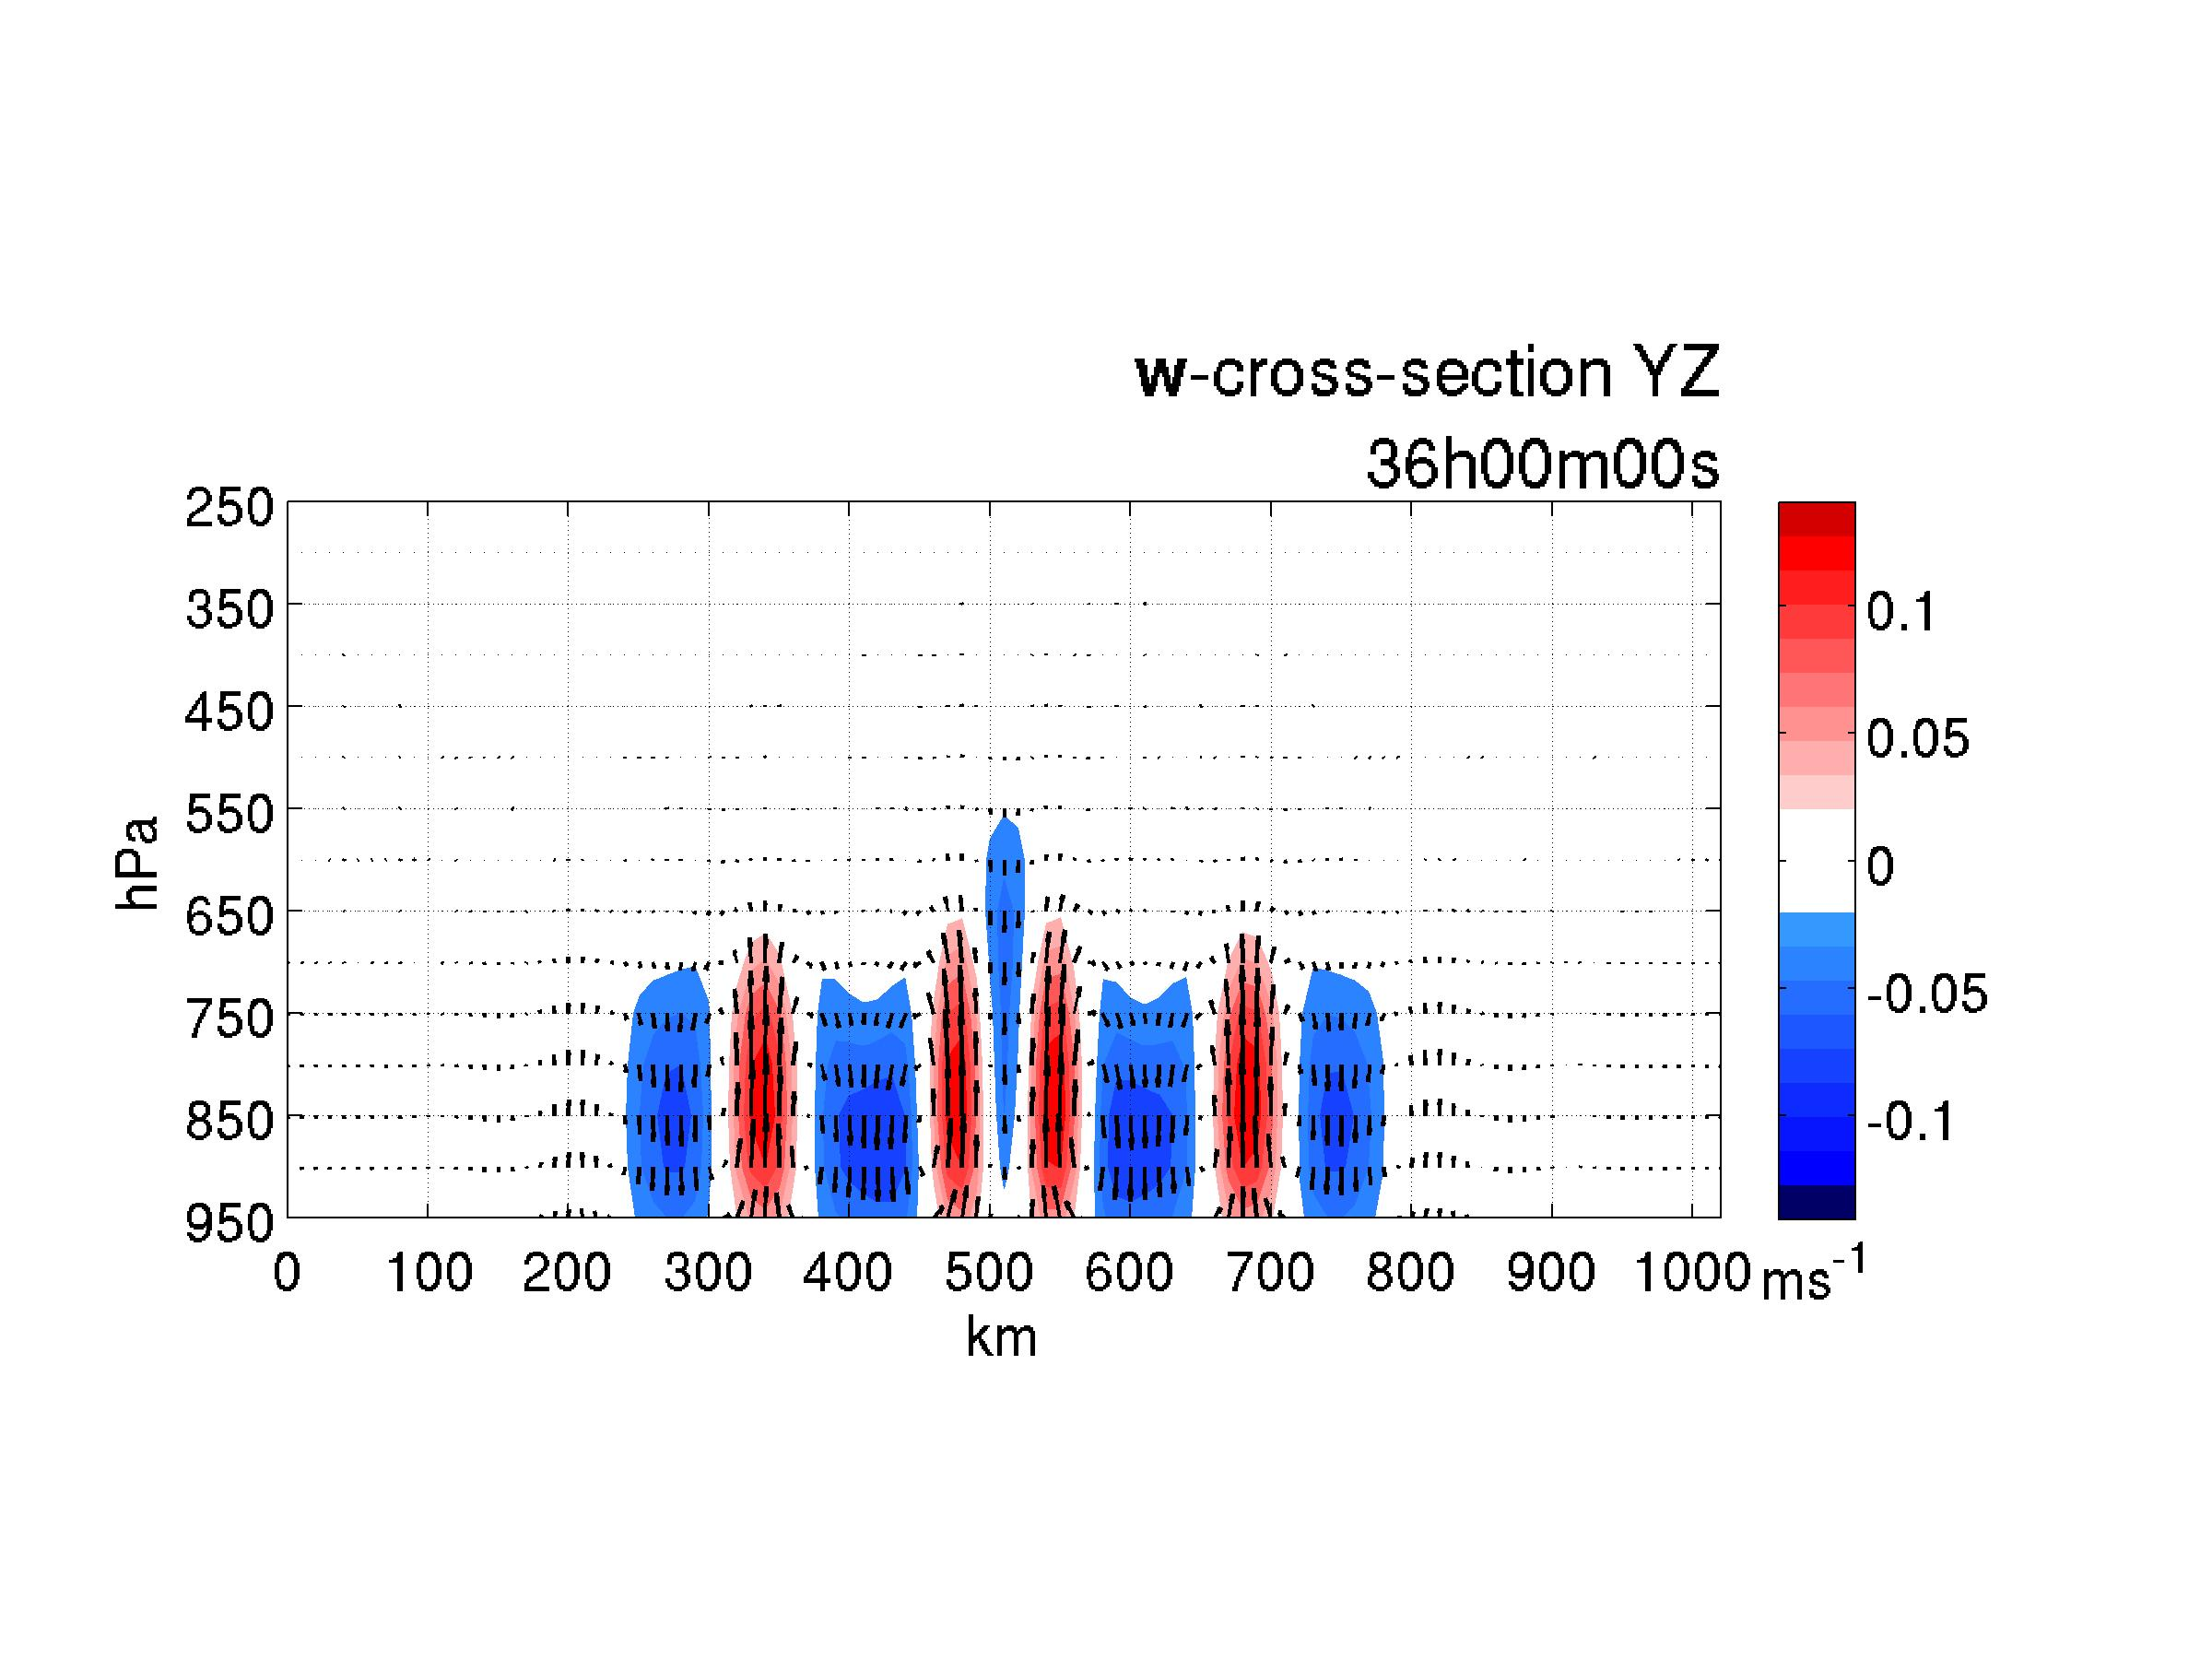
\includegraphics[width=\linewidth]{{./chapters/figures_results/W_cross_p.ix52.360000.FLAKE}.jpg}
%\vspace{-40pt}
%\caption{Зональный вертикальный разрез поля $w$-компоненты скорости (контуры) и значений вектора скорости (стрелки) в эксперименте M (36 ч.).}
%\label{fig:flake_wcross}
%\end{wrapfigure}
%
%Выявленные энергетической диагностикой различия между экспериментом M и остальными тремя экспериментами существуют из-за неодинакового воспроизведения конвекции в той или иной параметризации: параметризация M позволяет развитие свободной конвекции. Другими словами, в параметризациях потоков тепла по-разному заложена зависимость потока энергии с подстилающей поверхности от скорости ветра: при одинаковых скоростях приводного ветра поток явного тепла на радиусе максимального ветра в мезоциклоне отличается более, чем в 3 раза. Более того, в эксперименте M интерференция инерционно-гравитацинных волн порождает возникновение отдельных максимумов давления на периферии циклонического возмущения, что в дальнейшем приводит к распространению ячейковой конвекции во всей расчетной области. Размер отдельных конвективных ячеек (кроме центрального вихря) составляет $\approx 80\km$ в диаметре и $3500\m$ по вертикали (рис. \ref{fig:flake_wcross}).
%В качестве промежуточного вывода можно отметить, что использование параметризации Миронова (эксперимент M) дает более устойчивый мезоциклон и менее 'взрывной' его рост в конце эксперимента. По-видимому, различия в экспериментах сгладятся при условии, что атмосферные условия будут включать ненулевой фоновый поток. Сходство результатов в экспериментах L И BD дает право использовать параметризацию Бусингера-Дайера в дополнительных экспериментах \ref{sec:res:wishe}
%
%\subsection{CISK/WISHE для сухого (контрольного) и влажного эксперимента}
%\label{sec:res:wishe}
%Рассматриваемое циклоническое возмущение, очевидно, можно отнести к типу полярных мезоциклонов конвективного генезиса (энергия бароклинной или баротропной неустойчивости  здесь отсутствует). В разделе \ref{} были описаны две основные концепции роста полярного мезоциклона в результате термической неустойчивости --- CISK и WISHE. Глубже понять природу вихря и выявить, какой из этих механизмов интенсификации вихря доминирует в наших экспериментах, позволяет методика, хорошо описанная в \citep{CraigGray1996}. В обеих концепциях скорость роста циклона зависит от процессов в пограничном слое атмосфере: от потоков тепла и влаги в WISHE и от конвергенции в CISK. Определить, какой механизм доминирует в динамике циклона можно, варьируя параметры подстилающей поверхности: шероховатость в CISK и доступное количество тепла в WISHE. То есть ключевой момент методики заключается в том, что трение на поверхности изменяется независимо от турбулентных потоков явного и скрытого тепла. В численной модели это достигается изменением коэффициентов турбулентного сопротивления ($C_D$) и тепло- и влагообмена ($C_H$).
%
%Тесты на чувствительность вихря к коэффициентам турбулентного обмена проводились как для 'сухих' экспериментов (DRY), так и для 'влажных' (MOIST). На рис. \ref{} представлена КЭ для серии экспериментов, в которых $C_H$ уменьшался или увеличивался на $20$ и $50\%$. Большой разброс в полученных кривых указывает на сильную зависимость роста циклона от доступного тепла в приземном слое атмосферы: так, в экспериментах DRY значения КЭ отличаются более чем на порядок при изменении коэффициента на $50\%$. Несколько меньшую чувствительность обнаруживается в серии MOIST.
%
%Что касается влияния силы трения и конвергенции в центре вихря, то их роль незначительна (рис. \ref{}). Более того, повышение коэффициента сопротивления $C_D$ приводит лишь к увеличению стока КЭ, замедляя рост вихря, что не компенсируется более интенсивной экмановской подкачкой, особенно в экспериментах DRY. Систематического увеличения удельной влажности в пограничном слое атмосферы при увеличении $C_H$, необходимого в теории CISK Чарни и Элиассена, также не было выявлено.
%
%Чувствительность динамики вихря к потокам с поверхности можно оценить и с точки зрения углубления барической депрессии в центре. Интенсивность, определенная таким образом (см. \ref{}), в наглядно показана для $C_H$  на диаграмме \ref{}, а для $C_D$  на диаграмме \ref{}.
%
%Полученные результаты еще раз подтверждают, что циклоническое возмущение развивается благодаря взаимодействию океана и атмосферы по принципам теории WISHE. Вклад эффектов условной неустойчивости второго рода незначителен: область конвекции в вихре \emph{в центре} существует только в первые 18 часов, перемещаясь затем по направлению от центра вихря. Если бы влияние конвергенции и потока влаги в верхние слои было бы велико, то эффект изменения коэффициентов турбулентного обмена проявился бы в начале экспериментов.
%
%Результаты проведенных экспериментов качественно соответствуют результатам расчетов по осесимметричной модели \citep{CraigGray1996, EmanuelRotunno1989}. В отличие от указанной работы, тенденция к усилению вихря при увеличении коэффициента турбулентного обмена для тепла и влаги сохраняется даже при предельных значениях этого коэффициента (хотя и в меньшей степени в экспериментах MOIST). Стоит отметить, что для более уверенных результатов необходимо также рассмотреть динамику CAPE в районе развития вихря. В то же время в некоторых работах было установлено, что небольшое количество CAPE также может существовать при доминировании WISHE, также как, и при CISK-циклоне она тоже необязательно бывает большой. Кроме того, необходимо провести аналогичные серии экспериментов для других параметризаций потоков тепла и импульса.
%
%\section{Параметризация подсеточного перемешивания}
%Результат: в случае С-Л в КПС создается заметный 
%градиент пот. температуры, в случае же нелокального замыкания КПС 
%почти полностью перемешан и распространяется выше. Эксперимент
%с вихрем (но без потока $10\mps$) показывает, что вихрь затухает, не дотигнув и скорости $3\mps$. Это при фоновой стратификации $2\Kpkm$. При этом затухание выглядит, как увеличение размеров вихря с одновременным падением максимальной скорости. В области ненулевых скоростей ветра (т.е. в области циркуляции вихря), где есть поток тепла с поверхности, быстро образуется полностью перемешанный КПС. Думаю, теперь можно усилить факторы неустойчивости вихря (включить конденсацию, например), чтобы он развивался посильнее. В аналогичном эксперименте с замыканием С-Л вихрь развивается до $\approx 50\mps$, и превышается число Куранта.
%
%\subsection{Замыкание Смагоринского-Лилли (разный коэффициент турбулентности)}
%
%\subsection{Противоградиентное нелокальное замыкание}
%
%\subsection{Чувствительность к размерам температурной аномалии}
%Корректное моделирование полярных мезоциклонов в исследовательских или оперативных целях зависит не только от представления в модели фонового состояния атмосферы, но и от правильного задания параметров циклонического возмущения. Последнее можно показать на примере проведенной серии экспериментов, в которой варьировались радиус, высота и амплитуда температурной аномалии при ее инициализации \ref{}. Эволюция кинетической энергии в соответствующих экспериментах показана на рис.\ref{}--\ref{}, которые говорят о том, что эффект от изменения размеров или же амплитуды термического возмущения неодинаков. Оценивая результаты с точки зрения относительных изменениях $\theta_{max}$, $H$, $r_{out}$ на можно утверждать о низкой чувствительности вихря к высоте аномалии, средней чувствительности к горизонтальным размерам и сильной чувствительности к начальной температуре в центре. Так, при начальном максимуме температурного возмущения в $10\K$ продолжительность устойчивого эксперимента составила 1.5 сут., а при $\theta_{max}=2\K$ циклоническое возмущение не достигло значительной скорости и за трое суток.
%
%Такие же выводы можно сделать, сравнив изменение минимального давления \ref{}. Как и в описанных выше сериях экспериментов, построим зависимость интенсивности вихря от амплитуды начальной аномалии. Результаты количественной оценки чувствительности представлены в табл. \ref{}. 
%
%\section{Серия с разной скоростью фонового потока}
%В серии экспериментов, описываемых в данном подразделе, выясняется влияние фоновой скорости ветра на динамику циклонической аномалии. Как было сказано в \ref{sec:expplan:flow}, фоновый поток имеет строго зональное направление и однороден по пространству, а его скорость равна от $2$ до $10\mps$. При этом вихрь инициализировался на западе области.
%
%Все эксперименты качественно очень похожи друг на друга, отличаясь лишь скоростью роста КЭ \ref{} и временем достижения мезоциклоном боковых граней области, близи которых структура нарушается. На указанном рисунке видно, что КЭ рассматриваемых экспериментов ненулевая, так как это полная кинетическая энергия, включающая и средний поток. Рост КЭ начинает ускоряться в конце первых суток интегрирования, однако значения $dK/dt$ меньше, чем в контрольном эксперименте. С другой стороны, интенсивный рост циклонического возмущения начинается тем раньше, чем больше скорость начального (фонового) ветра. По-видимому, причиной такого соотношения является взаимосвязь циркуляции приводного ветра и потока явного тепла с поверхности: в эксперименте с сильным внешним воздушным потоком значения $H$ велики уже в первые часы существования циклонического возмущения (достигая $\approx 500\Wpermsq$).
%
%В бюджете КЭ среди слагаемых правой части преобладает $C(A,K)$, как и в контрольном эксперименте, но постепенно возрастает отрицательный вклад адвективных слагаемых, ответственных за поток энергии через боковые грани расчетной области \ref{}.
%Таким образом, процесс генерации ДПЭ и перехода ее в КЭ в данной серии экспериментов качественно не отличается от контрольного эксперимента. Это закономерно, так как начальное поле ветра не имеет градиентов скорости, а значит, фоновая атмосфера не является дополнительным резервуаром ДПЭ для атмосферных возмущений. Однако вклад фонового потока меняет структуру полярного мезоциклона. Скорость адвекции вихря оказывается приблизительно в 1.5 раза больше, чем фоновая скорость потока. Из-за этого с тыльной стороны циклона возникает своеобразный шлейф из волн, напоминающих волны обтекания орографического препятствия, а сам циклон приобретает форму запятой (рис. \ref{}). Кроме того, разделение циклонического возмущения на два мелких возмущения происходит более явно. Момент разделения отражается на эволюции полной КЭ в виде короткого плоского участка.
%
%%\begin{wrapfigure}{L}{0.5\textwidth}
%%\begin{center}
%%\includegraphics[width=\linewidth]{{./chapters/figures_results/ctrl_fields/pt_dev_z.x26-x76.y26-y76.ilev01.020000_}.jpg}
%%\end{center}
%%\caption{Поле отклонений температуры ($\theta'$) при инициализации возмущения (2 ч. модельного времени)}
%%\label{fig:initanom}
%%\end{wrapfigure}

\begin{thebibliography}{12}
 \bibitem{ER89}
Emanuel KA, Rotunno R. 1989. Polar lows as Arctic hurricanes. \textit{Tellus} \textbf{41A:} 1-17.
\end{thebibliography}

\end{document}
%\documentclass[12pt,a4paper]{report}
%%
% PACKAGES AND STYLES
%

% 
% Language and encoding
%
%\usepackage{mathtext}
%\usepackage[T2A]{fontenc}
\usepackage[utf8]{inputenc}
\usepackage[english,russian]{babel}
\usepackage{mmap}

%
% Colors
%
\usepackage[usenames]{color}
\usepackage{color}
\usepackage{colortbl}

%
% Symbols
%
\usepackage{amssymb}
\usepackage{MnSymbol}

%
% Units
%
%\usepackage[binary-units=true]{siunitx}
\newcommand{\km}{\mathrm{~\text{км}}}
\newcommand{\m}{\mathrm{~\text{м}}}
\newcommand{\s}{\mathrm{~\text{с}}}
\newcommand{\mps}{\m \s ^{-1}}
\newcommand{\pers}{\s ^{-1}}
\newcommand{\K}{\mathrm{~\text{К}}}
\newcommand{\Kpkm}{\K\km ^{-1}}
\newcommand{\hpa}{\mathrm{~\text{гПа}}}
\newcommand{\J}{\mathrm{~\text{Дж}}}
\newcommand{\Jpm}{\J \m ^{-3}}

%
% Paper size and margins
%
\usepackage{vmargin}
\setmarginsrb{2.5cm}{1cm}{2.5cm}{2cm}{0cm}{0cm}{0cm}{1.5cm}

%
% Page style
%
\usepackage{fancyhdr}
\setlength{\headheight}{16pt}
\newcommand{\changefont}{%
    \fontsize{9}{11}\selectfont
}
\fancyhf{}
\fancyhead[RO]{\changefont \slshape \rightmark} %section
\fancyhead[LO]{\changefont \slshape \leftmark} %chapter
\fancyfoot[C]{\changefont \thepage} %footer
\setlength{\headsep}{0.2in}
\pagestyle{fancy}

%
% Indenting
%
\usepackage{indentfirst}
\setlength{\parindent}{1cm}
\setlength{\parskip}{0.5cm}

%
% References
%
\usepackage{natbib}

%
% Hyperlinks
%
\usepackage[linktocpage=true,plainpages=false,pdfpagelabels=false]{hyperref}
\definecolor{linkcolor}{rgb}{0.1,0,0.9}
\definecolor{citecolor}{rgb}{0,0,0.9}
\definecolor{urlcolor}{rgb}{0,0,1}
\hypersetup{
    colorlinks, linkcolor={linkcolor},
    citecolor={citecolor}, urlcolor={urlcolor}
}

\bibliographystyle{plainnat}
% Bibliography: set article volume number in bold font
%\DeclareFieldFormat
%  [article]
%  {volume}{\textbf{#1}}
%\renewcommand\nameyeardelim{, }

%\usepackage{showkeys} % show labels

\newcommand{\figref}[1]{\mbox{Figure~\ref{#1}}}
\newcommand{\tabref}[1]{\mbox{Table~\ref{#1}}}
\newcommand{\secref}[1]{\mbox{Section~\ref{#1}}}
\newcommand{\chpref}[1]{\mbox{Chapter~\ref{#1}}}
\newcommand{\appref}[1]{\mbox{Appendix~\ref{#1}}}
\newcommand{\eqnref}[1]{\mbox{Eq.~(\ref{#1})}}
\newcommand{\listref}[1]{\mbox{Listing~(\ref{#1})}}

%
% Lists
%
\usepackage[shortlabels]{enumitem}

\newenvironment{sqlist}[1][\enskip$\filledsquare$]
        {\begin{itemize}[#1]}
        {\end{itemize}}

% New math commands
% differential d, from http://tex.stackexchange.com/a/60546/586
\newcommand*\diff{\mathop{}\!\mathrm{d}}
\newcommand\mean[1]{\overline{#1}}
\newcommand{\PDt}[2]{\partial #1/\partial #2}

%
% Tables
%
\usepackage{booktabs}
%\usepackage{tabularx}
\usepackage{tabu}
\usepackage{longtable}

%
% Figures
%
\usepackage{wrapfig}
\usepackage[font=small,textfont=it,labelfont=bf]{caption}
%\captionsetup[figure]{labelfont=bf}
\usepackage{tikz}
\usepackage{pgfplots}
\usetikzlibrary{calc}

%
% Equations
%
\usepackage{cool}

%\begin{document}
\chapter*{Заключение}
\addcontentsline{toc}{chapter}{Заключение}
\markboth{Заключение}{ }

Настоящая дипломная работа основывается на современных подходах к изучению полярных мезоциклонов и представляет собой анализ идеализированных численных экспериментов с использованием строгой энергетической диагностики. Подводя итоги, выделим основные результаты исследования:

\begin{enumerate}

\item Трехмерная негидростатическая модель ReMeDy была использована для воспроизведения формирования полярного мезоциклона конвективного характера в атмосфере при наличии или отсутствии эффектов выделения скрытой теплоты конденсации водяного пара. Была подробно рассмотрена структура осесимметричного циклонического возмущения, причиной возникновения которого являлась положительная аномалия потенциальной температуры воздуха вблизи поверхности. Динамика атмосферных движений была оценена с точки зрения уравнений баланса кинетической и доступной потенциальной энергии, а также в аспекте бюджета завихренности в нижней тропосфере.

\item С использованием общепринятой методики был сопоставлен вклад основных видов конвективной неустойчивости в эволюцию вихря. Установлено, что определяющим механизмом интенсификации полярного мезоциклона в проведенных экспериментах являлось взаимодействие атмосферы и океана в приводном слое атмосферы, описанное в теории WISHE.

\item По результатам нескольких серий численных экспериментов была выявлена зависимость интенсивности полярного вихря от некоторых параметров фоновой атмосферы и от характеристик начальной аномалии тепла. Чувствительность циклона к различным факторам была оценена количественно как отношение изменения интенсивности барической тенденции к изменению того или иного параметра. К параметрам атмосферы, рассмотренным в данном исследовании, относятся разность температуры воздуха и поверхности океана, влагосодержание воздуха, вертикальный градиент температуры, скорость фонового потока, а также амплитуда начального температурного возмущения. Чувствительность к начальному влагосодержанию оказалась довольно низкой, так как даже при пониженной относительной влажности в начале эксперимента в нижнем слое атмосферы быстро достигалось состояние насыщения. Средние показатели чувствительности к перечисленным факторам приведены в табл. \ref{tab:conclusions}.

\renewcommand{\arraystretch}{2}
\begin{table}
\centering
\caption{Чувствительность интенсивности вихря к параметрам фоновой атмосферы и амплитуде начальной аномалии температуры (значения на единицу изменения параметра).}
\label{tab:conclusions}
\small
\begin{tabu} to 0.8\linewidth {X[l]X[l]}
\toprule
Параметр, $P$ & Чувствительность, $\delta I/\delta P$ \\
\midrule
Уменьшение частоты Брента-Вяйсяля & $-1.03\hpa/\text{час}~(\pers)^{-1}$ \\
Увеличение разности температуры 'вода-воздух' & $-1.38\times 10^{-2}\hpa/\text{час}~\K ^{-1}$ \\
Увеличение скорости фонового потока & $-1.77\times 10^{-1}\hpa/\text{час}~(\mps)^{-1}$ \\
Увеличение начальной амплитуды & $-3.23\times 10^{-1}\hpa/\text{час}~\K ^{-1}$ \\
\bottomrule
\end{tabu}
\end{table}

\item На основе нескольких параметризаций потоков тепла и импульса с поверхности был оценен эффект использования схем перемешивания в приводном слое атмосферы. Было установлено, что наибольшее отличие вносит включение свободной конвекции, что отражается на циркуляции во всей расчетной области и снижает скорость роста центрального возмущения.

\item В модель ReMeDy была включена и успешно протестирована параметризация подсеточного перемешивания в пограничном слое атмосферы. Использование нелокального замыкания, учитывающего эффект противоградиентного переноса тепла в нижней тропосфере, показало на качественном уровне более близкое к данным наблюдений воспроизведение конвективного пограничного слоя атмосферы. Это сильно отразилось на динамике циклонического возмущения: при использовании улучшенного подсеточного перемешивания при прочих равных условиях мезоциклон развивался менее интенсивно, так, в 'сухой' атмосфере интенсификации вихря до ураганной силы не происходило.

\item Большое количество оценочных экспериментов требует дальнейшего совершенствования мезомасштабной численной модели ReMeDy. В ходе работы над представленным исследованием улучшения модели велись по таким направлениям, как:
	\begin{sqlist} 
		\item сбалансированная инициализация метеорологических полей для избежания генерации ложных волн;
		\item параметризация подсеточного турбулентного перемешивания;
		\item включение периодических граничных условий для возможности моделирования мезомасштабных циркуляций в зональных потоках; 
		\item способы инициализации начального возмущения;
		\item постпроцессинг данных моделирования.
	\end{sqlist}
	
Одним из факторов, к которым эксперименты оказались наиболее чувствительны, являются граничные условия. Вычислительная мода часто возникала на границах области, что возможно говорит о необходимости доработки горизонтальных и вертикальных численных фильтров.

\item Необходимы дальнейшие исследования чувствительности динамики мезоциклона к воспроизведению пограничного слоя и подсеточному перемешиванию атмосферы. Проблема правильного подбора схемы подсеточного перемешивания актуальна как для современных мезомасштабных моделей, используемых в оперативной практике, так и для глобальных моделей общей циркуляции атмосферы.

\end{enumerate}

%\end{document}


\appendix
\chapter{Основные аппроксимации и вывод системы прогностических уравнений модели ReMeDy \citep{MirandaPhD}}
\label{app:A}
Начнем с рассмотрения системы уравнений гидродинамики в невязком адиабатическом приближении в $z$-системе координат на $f$-плоскости:

\begin{subequations}\label{eq:eqn0}
\begin{align}
\frac{Du}{Dt}&=-\frac{1}{\rho}\pderiv{p}{x}+fv \label{eq:eqn1}\\
\frac{Dv}{Dt}&=-\frac{1}{\rho}\pderiv{p}{y}-fu \label{eq:eqn2}\\
\frac{Dw}{Dt}&=-\frac{1}{\rho}\pderiv{p}{z}-g \label{eq:eqn3}\\
\pderiv{u}{x}+\pderiv{v}{x}+\pderiv{w}{x}&=-\frac{Dln\rho}{Dt} \label{eq:eqn4}\\
\frac{Dln\theta}{Dt}&=0 \\
\intertext{\text{и уравнение состояния}}
p&=R\rho T, \label{eq:eqn5}\\
\intertext{\text{а потенциальная температура определяется как}}
\theta&=T\left(\frac{p_0}{p}\right)^\kappa. \label{eq:eqn6}
\end{align}
\end{subequations}

Далее в качестве вертикальной координаты примем
\begin{equation}
\sigma=\frac{p-p_{top}}{p_*}, p_*=p_{surf}-p_{top},
\end{equation}
которая превращается в традиционную $\sigma$-координату при $p_{top}=0$. В последующих выкладках примем, что $p_{top}$ есть константа. Производные в $\sigma$-системе коодинат соотносятся с производными в $z$-координатах следующим образом:
\begin{align}
\begin{split}
\left(\frac{\partial}{\partial x}\right)_z&=\left(\frac{\partial}{\partial x}\right)_{\sigma}-\left(\frac{\partial z}{\partial x}\right)_{\sigma} \left(\frac{\partial \sigma}{\partial z}\right) \left(\frac{\partial}{\partial \sigma}\right) \\
\frac{\partial}{\partial z}&=\frac{\partial\sigma}{\partial z}\frac{\partial}{\partial \sigma}
\end{split} \label{eq:z2sigma1}
\end{align}

Миллер и Уайт \citep{MillerWhite1986} получили систему уравнений в $p$-системе координат, применив ряд преобразований относительно связанного с фоновым состоянием параметром атмосферы, который имеет малые значения для широкого спектра атмосферных условий. Процедура может быть представлена в три этапа: \\
\begin{enumerate}
\item представление уравнений в новой системе координат, при это полагая $Dw/Dt$ параметром во всех уравнениях, кроме уравнения для вертикального ускорения;
\item определение фонового состояния как состояния гидростатического равновесия, в котором переменные зависят только от давления;
\item упрощение уравнений относительно фонового состояния с избавлением от членов высоких порядков.
\end{enumerate}

То есть фоновое состояние атмосферы определяется через переменные $$\phi_s(p), T_s(p)~or~\theta_s(p),$$
при чем
\begin{equation}
\frac{\partial\phi_s}{\partial\sigma}=\frac{\partial\phi_s}{\partial p}\frac{\partial p}{\partial\sigma}=-\frac{RT_s}{p}p_*
\end{equation}
Далее, следуя \citep{MillerWhite1986}, введем параметр
\begin{equation}
\epsilon=\frac{1}{g}\frac{Dw}{Dt},
\end{equation}
который является отношением вертикального ускорения к ускорению силы гравитации. Тогда уравнение для вертикальной скорости \eqref{eq:eqn3} может быть решено относительно $1/\rho$:
\begin{equation}
\frac{1}{\rho}=-\frac{g(1+\epsilon)}{\frac{\partial p}{\partial z}} \label{eq:vol}
\end{equation}

Подставляя последнее выражение в уравнения для горизонтальных компонент скорости \eqref{eq:eqn1} и \eqref{eq:eqn2} и используя \eqref{z2sigma:1}, получаем:
\begin{subequations}\label{eq:hmom0}
\begin{align}
\frac{Du}{Dt}&=\frac{g(1+\epsilon)}{\pderiv{p}{\sigma}\pderiv{\sigma}{z}}
\left[
\left(\pderiv{p}{x}\right)_\sigma-\pderiv{p}{\sigma}\pderiv{\sigma}{z}\left(\pderiv{z}{x}\right)_\sigma
\right]
+fv=g(1+\epsilon)
\left[\pderiv{\sigma}{p}\pderiv{z}{\sigma}\left(\pderiv{p}{x}\right)_\sigma-\left(\pderiv{z}{x}\right)_\sigma
\right]+fv=\nonumber\\
&=(1+\epsilon)
\left[
\frac{\sigma}{p_*}\left(\pderiv{p_*}{x}\right)_\sigma\pderiv{\phi}{\sigma}-\left(\pderiv{\phi}{x}\right)_\sigma
\right]+fv \nonumber \\
\intertext{or} \nonumber\\
\frac{Du}{Dt}&=(1+\epsilon)
\left[
-\left(\pderiv{\phi'}{x}\right)_\sigma+\pderiv{\phi'}{\sigma}\frac{\sigma}{p_*}\left(\pderiv{p_*}{x}\right)_\sigma
-\left(\pderiv{\phi_s}{x}\right)_\sigma+\pderiv{\phi_s}{\sigma}\frac{\sigma}{p_*}\left(\pderiv{p_*}{x}\right)_\sigma
\right]+fv \nonumber\\
\frac{Du}{Dt}&=(1+\epsilon)
\left[
-\left(\pderiv{\phi'}{x}\right)_\sigma+\pderiv{\phi'}{\sigma}\frac{\sigma}{p_*}\left(\pderiv{p_*}{x}\right)_\sigma
\right]+fv\label{eq:hmom1}
\intertext{and in a similar way:} \nonumber\\
\frac{Dv}{Dt}&=(1+\epsilon)
\left[
-\left(\frac{\partial\phi'}{\partial y}\right)_\sigma+\frac{\partial\phi'}{\partial\sigma}\frac{\sigma}{p_*}\left(\frac{\partial p_*}{\partial y}\right)_\sigma
\right]-fu\label{eq:hmom2}
\end{align}
\end{subequations}

Рассмотрим уравнение для вертикальной скорости \eqref{eq:eqn3}. Оно может быть переписано в виде
\begin{align}
g(1+\epsilon)&=-\frac{1}{\rho}\pderiv{p}{z} \\
\intertext{\text{или}} \nonumber\\
g(1+\epsilon)&=-\frac{1}{\rho}p_*\pderiv{\sigma}{z} \nonumber\\
(1+\epsilon)\left(\pderiv{\phi'}{\sigma}+\pderiv{\phi_s}{\sigma}\right)&=-\frac{1}{\rho}p_*\nonumber\\
\intertext{or, using the hydrostatic relation for the reference state:} \nonumber \\
(1+\epsilon)\left(\pderiv{\phi'}{\sigma}-p_*\frac{1}{\rho_s}\right)&=-\frac{1}{\rho}p_*\nonumber\\
-\epsilon p_*\frac{1}{\rho_s}-p_*\frac{1}{\rho_s}+(1+\epsilon)\pderiv{\phi'}{\sigma}&=-\frac{1}{\rho}p_*\nonumber\\
\epsilon p_*\frac{1}{\rho_s}&=(1+\epsilon)\pderiv{\phi'}{\sigma}+p_*\left(\frac{1}{\rho}-\frac{1}{\rho_s}\right)
\end{align}
Подставим $\epsilon$, согласно его определению, но только в первое слагаемое:
\begin{align}
\frac{Dw}{Dt}&=(1+\epsilon)\pderiv{\phi'}{\sigma}\frac{g\rho_s}{p_*}-g\frac{(\rho-\rho_s)}{\rho}\nonumber\\
\intertext{\text{и при} $\frac{\rho'}{\rho_s+\rho'}\approx\frac{\rho'}{\rho_s}$} \nonumber\\
\frac{Dw}{Dt}&=(1+\epsilon)\frac{g\rho_s}{p_*}\pderiv{\phi'}{\sigma}-g\frac{\rho'}{\rho_s} \label{eq:dwdt_rho}
\end{align}
Последнее слагаемое в правой части ур. \eqref{eq:dwdt_rho} может быть далее представлено как $g\frac{\theta'}{\theta_s}$.

С другой стороны, по определению вертикальное ускорение выглядит как
\begin{align}
\frac{Dw}{Dt}&=\frac{1}{g}\frac{D}{Dt}\left(\frac{D\phi'}{Dt}+\frac{D\phi_s}{Dt}\right)
\end{align}
и
\begin{align}
\frac{D\phi_s}{Dt}&=\pderiv{\phi_s}{p}\frac{D\phi_s}{Dt}=-\frac{RT_s}{p}\omega=-\frac{\omega}{\rho_s}.
\end{align}
Используя последнее, запишем:
\begin{align}
\tilde{w}&=\frac{1}{g}\frac{D\phi_s}{Dt}=-\frac{\omega}{\rho_sg} \\
\tilde{w}&=-\frac{1}{\rho_sg}\frac{Dp}{Dt}=-\frac{1}{S}(\dot{\sigma}+\frac{\sigma}{p_*}\dot{p_*}),
\end{align}
а окончательный вид уравнения для вертикальной скорости имеет вид
\begin{equation}
\frac{D}{Dt}\left[\frac{1}{g}\frac{D\phi'}{Dt}+\tilde{w}\right]=(1+\epsilon)S\pderiv{\phi'}{\sigma}+g\frac{\theta'}{\theta_s},
\end{equation}
где 
\begin{equation}
S=\frac{gp}{RT_sp_*}.
\end{equation}
Заметим, что 
\begin{equation}
-S\pderiv{}{\sigma}\approx\pderiv{}{z} \label{eq:dz}
\end{equation}

Преобразование уравнения неразрывности можно начать с рассмотрения уравнения, обобщенного на случай произвольной вертикальной координаты.
\begin{equation}
\frac{Dln\rho}{Dt}+\pderiv{u}{x}+\pderiv{v}{y}+\pderiv{\dot{\eta}}{\eta}+\frac{D}{Dt}\left(ln\left(\pderiv{z}{\eta}\right)\right)=0
\end{equation}
Имея в качестве вертикальной координаты $\sigma$-координату, получим уравнение неразрывности в системе координат модели:
\begin{equation}
\frac{Dln\rho}{Dt}+\frac{D}{Dt}\left(ln\left(\pderiv{z}{\sigma}\right)\right)+\pderiv{u}{x}+\pderiv{v}{y}+\pderiv{\dot{\sigma}}{\sigma}=0
\end{equation}
Используя опять уравнение \eqref{eq:vol}, переписанное в виде
\begin{equation}
\frac{D}{Dt}\left(ln\left(\pderiv{z}{\sigma}\right)\right)=\frac{Dlnp_*}{dt}-\frac{Dln\rho}{Dt}-\frac{Dln(1+\epsilon)}{Dt},
\end{equation}
получаем
\begin{equation}
\frac{Dlnp_*}{Dt}+\pderiv{u}{x}+\pderiv{v}{y}+\pderiv{\dot{\sigma}}{\sigma}=\frac{Dln(1+\epsilon)}{Dt}.
\end{equation}

Уравнение притока тепла может быть получено следующим образом. Сначала выпишем его в изобарических координатах:
\begin{equation}
\frac{D\theta}{Dt}=\frac{D\theta'}{Dt}+\frac{D\theta_s}{Dt}=\frac{D\theta'}{Dt}+\omega\pderiv{\theta_s}{p}=0.
\end{equation}
Далее, используя определение $\tilde{w}$ и свойства фонового состояния, получаем:
\begin{equation}
\frac{D\theta'}{Dt}-S\tilde{w}\pderiv{\theta_s}{\sigma}=0
\end{equation}
%which (neglecting the last term) can be written in a more familiar form, noting that:
%\begin{equation}
%-S\pderiv{}{\sigma}\approx\pderiv{}{z}
%\end{equation}
%and defining:
%\begin{equation}
%N^2=-S_v\frac{g}{\theta_s}\frac{\partial\theta_s}{\partial\sigma} \label{bfreq}
%\end{equation}
%leading to
%\begin{equation}
%\frac{g}{\theta_s}\frac{D\theta'}{Dt}+N^2\tilde{w}=0.
%\end{equation}

Система уравнений записана теперь в форме, удобной для упрощения, которое производится просто путем отбрасывания всех слагаемых, в которые входит параметр $\epsilon$ и величину $1/g\left(D^2\phi'/Dt^2\right)$. Миллер и Уайт обосновывают это приближение путем разложения членов уравнений в степенные ряды от малого параметра $\alpha$, зависящего лишь от фонового состояния. После чего отбрасываются члены высокого порядка и выводится система уравнений, подходящая для численного интегрирования. Условие, при котором описанная аппроксимация верна, следующее:
\begin{equation}
\alpha=\frac{\Delta\theta_s}{\theta_s}=\frac{p_0}{\theta_s}\pderiv{\theta_s}{p}\ll1,
\end{equation}
что всегда выполняется в тропосфере.
\addcontentsline{toc}{chapter}{\bibname}	% Добавляем список литературы в оглавление
\bibliography{diplomabib.bib}						% Подключаем BibTeX-базы

\end{document}
